% UTF-8 encoding

\documentclass{Thesis}
\setlength{\headheight}{15pt}
\begin{document}    

\frenchspacing % disable specific space after coma
\raggedbottom %  makes all pages the height of the text on that page. No extra vertical space is added.
\pagenumbering{roman}
\pagestyle{plain}

\arrayrulecolor{chaptergrey} % stroke color for tables 

% the front matter
\frontmatter 
% some details about the thesis
\title{This is the title of the thesis}
\author{Author's name}
\advisor{Advisor's name}

% about the degree
\degree{Doctor of Philosophy}
\field{Subject}
\degreeyear{Year}
\degreemonth{Month}

% about the university
\department{Department}
\university{Harvard University}
\universitycity{Cambridge}
\universitystate{Massachusetts}
\maketitle
\copyrightpage

\abstractpage
\addcontentsline{toc}{section}{Abstract}

\acknowledgments
\addcontentsline{toc}{section}{Remerciements}

\sommaire
\addcontentsline{toc}{section}{Sommaire}

% the main course
\mainmatter
\begin{spacing}{1.5} % line spacing

\chapter*{Introduction}

% 1. contexte : planter le décor

\newthought{Parler, partager, commenter, discuter, écrire} sont les actes quotidiens qui font circuler les informations sur l'Internet. Du silicium des serveurs aux écrans des téléphones, des millions de messages se frayent chaque jour des chemins insoupçonnés à travers les multiples plate-formes du Web. Soutenues par l'appétit d'une industrie florissante, ces nouvelles formes de conversation viennent interroger et renouveler les pratiques médiatiques, politiques, scientifiques et managériales.

Les \textit{mèmes Internet}, petites blagues circulant rapidement sur la Toile, réunissent autour d'eux un grand nombre d'utilisateurs en un temps très court. Satire politique, action commerciale ou simple blague potache, la vélocité et le pouvoir fédérateur de ces simples photos légendées ne cessent de surprendre. Les modèles de leur diffusion, encore largement méconnus, ont jusqu'ici été essentiellement compris par analogie avec ceux du virus biologique. Pourtant, l'observation des tensions entourant l'appropriation de ces puissantes instances médiatiques donne à voir une réalité bien différente.

Ces objets numériques atypiques ont également pénétré les fenêtres des navigateurs Internet en Chine, portés par le sarcasme et l'humour. Le service de microblog \textit{Weibo} lancé par le portail \textit{Sina} a connu un dès son lancement en 2008 un succès fulgurant. La réactivité de ce service de publication instantanée a démultiplié les espaces de conversation en ligne. Rassemblant aujourd'hui plusieurs centaines de millions d'utilisateurs, cette plateforme a amené de nouvelles pratiques de la discussion au sein d'un environnement médiatique chinois traditionnellement très contrôlé \citep{MacKinnon2009, Douzet2007, Yang2008}

La croissance rapide de \textit{Sina Weibo} a été largement soutenue par la politique du gouvernement central de Pékin. Le protectionnisme strict appliqué au secteur des industries culturelles et des Technologies de l'Information et de la Communication (TIC) a notamment permis à la firme de se développer dans un environnement non-concurrentiel. Ses homologues américains \textit{Twitter} et \textit{Facebook} ont en effet été bannis du paysage chinois, rendus inaccessibles depuis l'intérieur du territoire \citep{Sullivan2012}. La valorisation importante sur les marchés d'affaires du titre \textit{Sina}\footnote{D'après \url{http://finance.yahoo.com/echarts\?s=SINA+Interactive\#symbol=SINA;range=5y}, consulté le 5 Juillet 2014 à 11h10} témoigne du succès économique et commercial de l'entreprise. Néanmoins, l'évolution des régulations et utilisations du service lui-même témoigne des tensions constantes entre agenda gouvernemental, désir d'expression des utilisateurs et objectif de rentabilité.

% objectifs
La présente recherche se propose d'examiner les différents régimes d'expression et de discours régissant les usages de \textit{Sina Weibo} grâce à l'étude des contenus à forte circulation - dont les mèmes. Les travaux concernant cette plateforme se polarisent souvent autour des actions de marketing, des stratégies de censure gouvernementale \citep{Ng2013a} ou des tactiques de contournement développées par les utilisateurs \citep{Yang2014}. Nous souhaitons ici dépasser ce clivage en considérant la complexité des relations entre pouvoir politique, industries culturelles et pratiques quotidiennes afin de proposer une lecture plus contrastée \citep{Fernandez2010}.

Pour ce faire, nous dresserons un portrait de différents contenus web sur \textit{Sina Weibo} comprenant mèmes absurdistes, scandales politiques, débats de société et campagnes commerciales. Un outil d'analyse et de visualisation de données spécialement conçu 
% pour l'occasion
nous permettra d'observer dans le détail les interactions entre plate-formes, mots, lieux et utilisateurs lors de leur diffusion.


\subsubsection{Modèles théoriques de la diffusion sur les réseaux sociaux}

% vision globale
L'analyse des activités humaines grâce aux informations disponibles en ligne promet de devenir une ressource méthodologique importante dans de multiples champs scientifiques \citep{Schreibman2007}. Stockées en des lieux et formats pas toujours aisément accessibles, ces fragments s'amoncèlent pour former d'innombrables bases de données. Parfois désignées par le mot-valise de \textit{Big Data} \citep{Lohr2012a}, ces traces matérielles pourraient permettre une forme nouvelle d'archéologie des phénomènes humains. L'accès et le traitement de cette mémoire technologique nécessitent un renouvellement de l'écriture scientifique, utilisant à la fois les langages humains et informatiques \citep{ Guichard2014}. La fiabilité des méthodes et la pertinence des découvertes issues de ce vaste champ d'expérimentations restent encore largement à construire \citep{Boyd2011}.

Les données produites par l'usage des services de réseaux sociaux offrent notamment une opportunité nouvelle pour l'étude des pratiques de communication \citep{Zook2007,Nettleton2013,Manovich2011}. La disponibilité en grande quantité de matériels retraçant les échanges quotidiens les plus divers augure de nouvelles formes d'investigation et d'analyse. Depuis la sociométrie de \cite{Moreno1938}, le modèle des réseaux a progressivement structuré la lecture des phénomènes sociaux \citep{Latour1999a, Castells1989}. Guidé par les théories de la complexité \citep{Morin1990}, cette science des réseaux émergente \citep{Brandes2013} trouve un terrain de prédilection dans l'analyse des activités sur les réseaux sociaux en ligne. L'observation des dynamiques entourant la diffusion des conversations en ligne fait notamment l'objet de nombreux travaux d'une grande variété méthodologique : modélisation statistique \citep{Steyer2006}, cartographie \citep{Conover2013,Eisenstein2012},  simulation \citep{Tubaro2010}, etc. 

% la logique sous-jacente du travail
L'analyse des données conversationnelles issues des réseaux sociaux souffre cependant d'assises théoriques encore peu élaborées. La visualisation de conversations sous forme de graphes d'utilisateurs est couramment utilisée dans les travaux sur la communication en ligne. Cette schématisation modélise pourtant les échanges entre individus selon un schéma émetteur-récepteur très basique et largement décrié \citep{Proulx2000}. Les réflexions théoriques et méthodologiques sur l'analyse communicationnelle des données provenant de réseaux sociaux émanent le plus souvent de disciplines connexes comme la géomatique \citep{Crampton2013, Leetaru2013} ou l'informatique \citep{Brodka2013, Russel2011}. Notre travail s'efforce de situer ces pratiques dans une perspective historique. Par conséquent, nous avons été amené à faire dialoguer des approches conceptuelles diverses (espaces, territoires, lieux, rhétorique, discours, énonciation, code...) issues de champs disciplinaires multiples (communication, gestion et systèmes d'information, géographie des technologies, histoire du langage, etc.)

% raison d'être de la recherche
Notre réflexion est conduite autour de l'idée de \textit{milieu numérique}, construit des protocoles et interfaces technologiques, physiques et institutionnels du web \cite{Hui2012}. L'actualisation de ce milieu numérique par la circulation de formes spécifiques de contenus dessine des motifs particuliers que nous nommons \textit{topogrammes}. Ces topogrammes sont connaissables par l'observation des propriétés des structures sémantiques, topologiques et spatio-temporelles représentant le mouvement des informations dans le réseau. Mèmes humoristiques, campagnes publicitaires ou scandales politiques, chaque contenu peut être abordé par la forme particulière de son topogramme, expression de son ou ses milieux numériques.


\subsubsection{Outil d'observation et de visualisation de données}

% suppositions / postulats
Le terme de \textit{mème}, défini initialement comme une unité de diffusion culturelle, trouve son origine dans une analogie avec le gène biologique \citep{Dawkins1989, Blackmore2001}. La dimension évolutionniste sous-jacente du mot et l'absence de domaines d'application l'ont cantonné pendant longtemps aux marges de la culture scientifique \citep{Jouxtel2014}. Remis au goût du jour avec l'Internet, les mèmes ont depuis été le sujet de plusieurs études, utilisant souvent le virus comme modèle idéal de la diffusion des contenus sur les réseaux sociaux \citep{Leskovec2005, Adamic2014}. L'idée d'une transmission mécanique par contact représente peu la réalité entrant en jeu dans l'appropriation d'objets technologiques \citep{Orlikowski1993} ou informationnels \citep{Certeau1980}. De plus, naturaliser des éléments de culture commune en entités autonomes nous semble non seulement réducteur mais aussi dangereux \citep{Elias1975}.

% méthodologie % approche
Aussi nous éloignons nous de la description virale du mème pour observer en détail les topogrammes de différents objets numériques en concevant un dispositif de visualisation de données. À la croisée de l'ingénierie et de la réflexion méthodologique, nous utilisons les technologies de l'analyse des réseaux conversationnels \citep{Weng2012}, du traitement automatique de la langue chinoise \citep{Xue2003} et de la visualisation d'information \citep{Cairo2012}. Nous sélectionnons des contenus de différents types sous la forme de jeux de messages extraits d'un vaste corpus de 200 millions d'interactions retranscrivant l'activité de \textit{Sina Weibo} durant l'année 2012 \citep{Fu2013}. Notre dispositif permet ensuite de montrer différents aspects de leur circulation au sein d'un seul et même espace de représentation.

% son domaine d'application
Cette réflexion s'ancre dans le contexte politico-économique chinois avec le cas particulier de \textit{Sina Weibo}. Nous discuterons du rôle de l'industrie médiatique et des enjeux politiques agissant dans la formation des pratiques en ligne. Nous chercherons également à formuler des recommandations pratiques et méthodologiques concernant la création et l'analyse d'objets digitaux à forte diffusion. Notre dispositif technologique est spécialement conçu avec pour finalité la ré-utilisation sur d'autres terrains, domaines et plate-formes.


\subsubsection{Plan de la thèse}

% l'évolution de sa réalisation
% appréhender le contenu de la thèse.
La première partie de cette thèse présentera l'exemple historique du développement de l'Internet en Chine et plus particulièrement du service de microblog \textit{Sina Weibo}. Nous introduirons le concept de \textit{milieu numérique} pour problématiser les rapports existants entre protocoles et usages dans le contexte d'Internet.

La seconde partie discutera la notion de \textit{mème Internet} en proposant une première typologie des différents usages exprimés par ce mot mystérieux. Nous introduirons l'idée de \textit{topogramme} afin de décrire les structures observables lors de la diffusion en ligne.

La partie suivante introduira des réflexions épistémologiques et méthodologiques relatives à l'analyse et au traitement de larges jeux de données issues des réseaux sociaux. Nous discuterons la possibilité d'identifier des mèmes grâce à un protocole expérimental mobilisant différentes approches algorithmiques.

La dernière partie présentera dans le détail les choix retenus lors du développement de notre outil d'analyse et de visualisation. Un échantillon d'une douzaine de mèmes sélectionnés permettra de présenter et discuter les figures obtenues grâce à cet outil. Nous établirons des catégories d'après les modèles de circulation des contenus sur \textit{Sina Weibo}. Enfin, nous nous interrogerons sur la portée et la validité des méthodes d'analyse de données en sciences humaines au regard des résultats de la présente recherche.

\addcontentsline{toc}{chapter}{Introduction}

\chapter{Sina Weibo et le milieu numérique en Chine} 

\newthought{Géant de l'Internet}, la Chine constitue aujourd'hui une des plus grandes figures de l'ordre médiatique mondial. Avec plus de 538 millions d'internautes recensés\footnote{En Juin 2012 d'après  \url{http://www.internetworldstats.com/asia.htm}, consulté le 12 juin 2014 à 14:05}, la présence du Web chinois pèse non seulement dans la balance démographique, mais aussi dans la lecture des fondements politiques du réseau. En effet, le discours et les motivations techno-idéologiques qui ont présidé au développement de l'Internet en Chine diffèrent largement de ces précédents américains et européens. 

Le regard historique que nous allons porter dans la première partie de ce travail rend compte de la lecture des enjeux industriels et politiques qu'ont porté les cadres du Parti Communiste Chinois (PCC) sur les réseaux d'information. La fermeture de \textit{Facebook}, \textit{Youtube} ou \textit{Twitter} relève en effet autant du protectionnisme économique que de la censure médiatique. L'exemple du service de microblog chinois \textit{Sina Weibo}, qui sera l'objet de notre étude, est sans doute un des exemples les plus parlants des bénéfices apportés par le protectionnisme économique aux industries culturelles chinoises. La réussite commerciale de la firme \textit{Sina}, la surveillance constante exercée par le gouvernement et la  possibilité pour les utilisateurs de dialoguer librement sur le service \textit{Weibo} forment un mélange atypique et détonnant que nous allons maintenant décrire.

Tour à tour espace, lieu et territoire, cette plate-forme web articule  différents intérêts et usages dans des dynamiques parfois antagonistes. Cette complexité prend corps dans l'existence géographique de ce réseau en Chine. Une relecture historique de l'évolution du concept de milieu nous amène à proposer le concept très simondonnien de \textit{milieu numérique} pour décrire l’ensemble des protocoles et pratiques discursives qui préside à la création des objets numériques. Nous discuterons également son actualisation sous des forme spécifiques appelées \textit{topogrammes}.


\section{L’Internet chinois : éléments de contexte }
\label{sec:internet-chine}
La production de la recherche en sciences sociales s'est longtemps concentrée autour des intérêts politiques et économiques qui entourent les usages et les modes de diffusion de l’Internet en Chine. Les premières études académiques sont issues du champ de l’information-communication et plus spécifiquement du monde anglo-saxon \citep{Johnson1996,Qiu2005}. Leurs approches reposent sur le postulat qu'Internet serait un outil favorisant la démocratisation. Ainsi cette littérature peut se résumer en un échange d'arguments autour d'une alternative : l'entrée de la Chine dans la ``société de l'information'' va de pair avec la modernisation économique et la démocratisation ou à l’inverse avec un contrôle politique accru de l'information et de la société. Les autorités chinoises craignent en effet de voir se développer de nouveaux canaux de circulation et de nouvelles sources d'information échappant à leur autorité traditionnelle sur les médias - et contestant ainsi leur pouvoir. D'un autre côté, le média internet est également perçu par le gouvernement comme un agent indispensable du processus de modernisation politique et économique (dont l’ouverture de marchés commerciaux intérieurs) permettant de faire circuler l’information de façon optimale, en touchant ainsi l’ensemble des foyers. En somme, un Internet ``sain'' et maîtrisé soutiendrait le développement du système de valeurs gouvernemental, mais également de l’économie et de la culture. Ici, de nombreuses publications se sont également intéressées au rôle de l’économie en ligne dans la croissance économique de la Chine et aux liens étroits des entreprises web avec la censure \citep{Dann2008}. Ces questions de liberté d’expression et du rapport entre démocratie et médias occupent encore aujourd’hui une large place dans la littérature \citep{MacKinnon2009, Douzet2007, Yang2008}.

Les études propres aux usages d’Internet dans le contexte chinois sont toutefois moins nombreuses ou sont généralement le fruit des services marketing des entreprises locales ou internationales en quête de nouveaux marchés \citep{Hwang2005, Bergstrom2012}. Toutefois, on retrouve à la croisée de ces différentes discussions des études plus précises qui cherchent à mettre en relation les dimensions à la fois économique et d’usage du web chinois \citep{Puel2009, Fernandez2010}. Dans le domaine précis de l’analyse des réseaux sociaux - en anglais \textit{Social Network Analysis} (SNA), les publications internationales en sciences sociales concernant la Chine restent encore peu nombreuses. Le champ de la recherche en informatique propose plusieurs études décrivant les dynamiques des échanges de contenus \citep{Yu2011} et les dispositifs de censure en place sur \textit{Sina Weibo} \citep{Bamman2012}. 

Afin de mieux se situer dans le large paysage de cette littérature, cette première partie rend compte des principaux éléments historiques, politiques et économiques d’infra et d’infostructure de l’internet chinois.

\subsection[Petite histoire et évolution de l’Internet chinois]{Petite histoire et évolution de l’Internet chinois}

L’Internet chinois est aujourd’hui le plus grand réseau national, dépassant depuis 2011 l’Amérique du Nord et l’Europe réunies \citep{CNNIC2013}\footnote{538 millions d'utilisateurs alors même que seuls 40\% de ses habitants disposent à ce jour d’une connexion : \textit{`` La collection des données se fait grâce à des logiciels, questionnaires en ligne et sondages par téléphones (…) Pour le CNNIC, un internaute est un citoyen chinois agé de plus de 6 ans qui utilise Internet au moins une heure par semaine ou a utilisé Internet durant les 6 derniers mois ''} (d’après le site officiel de CNNIC, agence officielle du gouvernement).}. Alors que l’installation des infrastructures a débuté seulement en 1996, l’expansion en a été fulgurante \citep{Fang2006}. 51 millions de nouveaux internautes chinois ont fait leur apparition en 2012, soit une hausse de 10\% par rapport à 2011 \citep{CNNIC2013}. 

Comme ailleurs dans le monde, les débuts des réseaux informatiques en Chine se déroulent dans le contexte universitaire avec la création en 1994 du CERNET (\textit{China Education and Research Network}) permettant de relier plusieurs grandes universités du pays. Le 17 mai 1994, la Chine effectue sa première connexion au réseau Internet en se reliant au \textit{Stanford Linear Accelerator Center} (SLAC) de l’Université de Stanford aux États-Unis. L’année suivante, les infrastructures \textit{backbones} nécessaires à l’installation de l’Internet à plus large échelle sont déployées (ChinaNet, GBNet, CERNET) et la première licence d’exploitation commerciale est attribuée, effective dès 1996. Le 1er janvier 1997, le \textit{Quotidien du Peuple} lance sa première version en ligne, devenant alors le premier site Internet d’information officielle du pouvoir central Chinois sur Internet. Dans le courant de l’année, le premier FAI privé chinois \textit{China InfoHighway} voit le jour. En Novembre, le CNNIC (\textit{China Internet Network Information Center}) est chargé de recueillir et publier des statistiques sur le développement de l’Internet en Chine \citep{Dai2007}.

Dès son commencement, la mise en place et le contrôle du réseau Internet sont des enjeux importants pour le gouvernement de Pékin. Partie intégrante de leur programme de gouvernance, les dirigeants communistes ont appris depuis longtemps à considérer très sérieusement les nouveaux outils de communication, à la fois comme un risque et une opportunité. Le plus célèbre témoin de cette histoire est sans doute le cinéma soviétique mis en place par Lénine et Trotski dès leur arrivée au pouvoir en 1917. Les \textit{agitki}, courts films de propagande, révèleront de grands cinéastes comme Koulechov, Vertov ou même Eisenstein \citep{Mazuy2002}. Au début des années 90, la Chine s’est engagée depuis plus de 10 ans dans de vastes réformes (\textit{gaige kaifang}) pour se sortir de l’état de chaos où l’avait laissé la Révolution Culturelle. La politique d’ouverture du pays couplée à un fort protectorat ouvre l’ère du \textit{Made in China} qui concerne l’ensemble des secteurs industriels, y compris ceux des médias et télécommunications dont le potentiel stratégique et économique est énorme. Les dirigeants de Pékin sont également bien conscients que la place forte que la Chine réclame dans le paysage mondial se dessinera notamment par une intégration accrue dans le réseau mondial des TIC. Ainsi, en Mars 2000 alors que la population des internautes chinois atteint 16,9 millions d’internautes, le premier ministre Jiang Zemin affirme : \textit{“Internet technology is going to change the international situation, military combat, production, culture, and economic aspects of our daily life significantly.”} \citep{Foster2000}

Alors qu’Al Gore et l’administration Clinton déploient les \textit{“information superhighways”} aux États-Unis, le programme d’informatisation et de développement des Technologies de l'Information et de la Communication (TIC) \textit{xinxihua}  devient une des clés du calendrier politique et économique chinois. Jiang Mianheng, le fils du premier ministre Jiang Zemin, est chargé du déploiement de ce vaste projet. Revenu en 1992 après plusieurs années passées dans les universités américaines puis dans la Silicon Valley chez \textit{HP}, Jiang Manheng investit largement dans les infrastructures et soutient dès 1999 le lancement du haut-débit en Chine avec la compagnie \textit{Netcom}, aujourd’hui encore deuxième opérateur du pays \citep{Dai2007}. Fortement influencé par les théories de Alvin Toffler \citep{Tsui2007}, le gouvernement de Jiang Zemin est bien décidé à ne pas rater la \textit{“troisième vague”} de modernisation de l’industrie : l’informatisation. La mise en place d’une quinzaine de \textit{“golden projects”} informe le mouvement de stratégie globale qui doit dynamiser transversalement tous les secteurs d’activité jusqu’au au sein-même de l’administration chinoise. Alors que les \textit{“golden customs”} se chargent des données du commerce extérieur et que la \textit{”golden sea”} devient un outil de communication entre cadres du Parti et administrations locales, les multiples \textit{“golden projects”} sont soutenus par la volonté de mettre en place un \textit{e-government}. Pékin veut faire de l’Internet chinois un espace de dialogue entre citoyens et organes du gouvernement grâce notamment à la mise en place de services administratifs en ligne et d’enquêtes transversales sur la qualité de vie dans les différentes villes de Chine. La gestion proactive de l’Internet national offre également au Parti un vecteur unique pour la diffusion de ses idées politiques. Plusieurs études montrent comment les idées et discours nationalistes sur l’Internet ont bénéficié d’un soutien constant du gouvernement chinois, avec notamment comme objectif l’accès aux communautés chinoises émigrées à l’étranger \citep{Hughes2000}. Finalement, le média Internet doit servir les intérêts du gouvernement et participer à l’unification territoriale, à l’instar des autres médias dits traditionnels comme la télévision.

\subsection[Censure sur l’Internet chinois]{Censure sur l’Internet chinois}
Les modes d’adoption de la technologie Internet par le gouvernement de Pékin illustrent pourtant bien le dilemme constant entre ouverture et protectionnisme qui tiraille la classe politique chinoise depuis la fin de la Révolution Culturelle. L’ouverture au monde et la politique de réformes du \textit{"nouveau départ"} s’accompagnent pour la Chine de nombreux défis souvent considérés comme extérieurs, que résume avec clarté une phrase célèbre attribuée à Deng Xiaoping : \textit{"Lorsque vous ouvrez une fenêtre pour avoir de l’air frais, vous devez vous attendre à ce que quelques mouches rentrent dans la pièce."} Alors que les promesses d’expansion économique et politique de l’Internet sont bien au rendez-vous, les “mouches” entrées par les fenêtres des navigateurs web commencent à essaimer pour faire de plus en plus bruit. 

Depuis 1998, le Ministère de la Sécurité Publique chinois travaille à la conception d’un projet intitulé \textit{Golden Shield} qui constituerait un fichier global des citoyens chinois utilisable tant pour le contrôle de la démographie que le vol de véhicules ou la sécurité aux frontières \citep{Lyons2009}. Lors d’un Trade Show intitulé \textit{"Security China 2000"} se déroulant à Pékin en 2000, le projet est présenté publiquement comme une large base de données devant regrouper les informations administratives des citoyens et leurs activités en ligne dans le but de favoriser le travail de la police \citep{Walton2001}. Titanesque et complexe à réaliser, le projet est peu à peu modifié pour devenir un système de filtrage de contenus et de blocage de sites, basé sur le système du \textit{firewall}. Fang Binxing, un professeur spécialisé dans la sécurité informatique à l’Université de Harbin, est nommé chef-ingénieur du projet \textit{Golden Shield}. Il recrute de nombreux ingénieurs et avec l’aide de l’université de Qinghua et de plusieurs entreprises occidentales (Nortel Networks\footnote{\textit{“Nortel Networks signs contracts valued at over USD 120 Millions during Canadian Prime Minister Jean Chretien’s visit to China”}, PR Newswire, \url{http://www.prnewswire.co.uk/news-releases/nortel-networks-signs-contracts-valued-at-over-us-dollars-120-million-during-canadian-prime-minister-jean-chretiens-visit-to-china-156751255.html}, consulté le 17 Février 2014 à 12:18}, Cisco \footnote{\textit{“Cisco Leak: ‘Great Firewall’ of China Was a Chance to Sell More Routers”}, 
Sarah Lai Stirland, 05.20.2008, \url{http://www.wired.com/threatlevel/2008/05/leaked-cisco-do/} consulté le 17 Février 2014 à 12:39}). Ensemble, ils s’attèlent au développement technologique du projet qui devait devenir le système de contrôle de l’Internet chinois aujourd’hui en activité. Baptisé de manière informelle \textit{“The Great Firewall”} (GFW) par analogie avec la \textit{"Grande Muraille de Chine”} (Great Wall), ce système `` sociotechnique '' hors du commun est aujourd’hui considéré comme une des plus grandes installations d’analyse et de traitement de données en activité. À chaque seconde, GFW traite et scanne des millions de chaines de caractères issues des requêtes et pages vues par des centaines de millions d’internautes \citep{Winter2012}. Au-delà de la censure automatique, GFW emploierait aujourd’hui entre 30 000 et 50 000 personnes\footnote{\textit{"What is internet censorship?"}. Amnesty International Australia. 28 Mars 2008. Consulté le 17 Février 2014 à 15h12} : ingénieurs, modérateurs, relecteurs, officiers de police, etc. Phénomène particulier, un groupe de rédacteurs est notamment chargé d’intervenir dans les discussions ou les forums en ligne pour faire valoir le point de vue officiel. L’adage veut que chacun des messages posté soit rémunéré 50 centimes RMB, ce qui a amené les internautes chinois à baptiser non sans humour ces représentants de l’ordre politique en ligne \textit{“le Parti à 50 centimes” (wumao dang)}.

\begin{figure}[htbp]
    \centering
    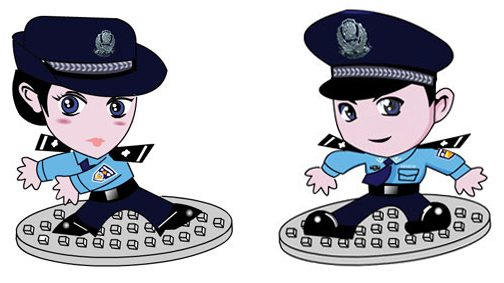
\includegraphics{figures/chap1/jingcha.jpg}
    \caption[Jingjing et Chacha, les policiers de l'Internet chinois]{\textit{Jingjing} et \textit{Chacha} sont deux figures créées par les autorités chinoises pour signifier la présence policière en ligne aux internautes. Le nom de ces veilleurs dessinés est une composition issue du mot “police” en chinois (\textit{jingcha}). Source : \url{http://jswm.newssc.org/system/2008/10/29/011233423.shtml} consultée le 17 Février 2014, à 15:32}
    \label{fig:jingcha}
\end{figure}

Au-delà de l’activité manuelle de milliers d’employés, GFW opère également plusieurs types de blocages sur les contenus. Techniquement, la plupart des filtrages se déroulent au niveau du fournisseur d’accès avec notamment des adresses particulières qui sont rendues inaccessibles : l’adresse \textit{facebook.com} ou \textit{youtube.com} renvoie une erreur “404 : Le site demandé n’existe pas”. Ainsi, de nombreux sites célèbres ne sont pas accessibles (\textit{Twitter}, \textit{Youtube}, \textit{Facebook}, etc.) Les autres blocages effectifs s’effectuent selon les adresses IP ou les serveurs d’attribution de noms de domaine (DNS) menant parfois au blocage de serveurs entiers \citep{Winter2012}. Les URLs des pages de certains sites importants sont également filtrées. Sur Wikipedia notamment, la page \textit{“Tiananmen Square protests of 1989”} est inaccessible depuis la Chine sans que le site Wikipedia soit pour autant intégralement bloqué. Également, des requêtes contenant des mots “interdits” sur les moteurs de recherche peuvent conduire à des micro-coupures ou un accès restreint au web pendant parfois plusieurs minutes\footnote{Testé depuis Shanghai en Septembre 2013.}. La liste des sites et mots bloqués n’est pas publiée par le gouvernement et l’ajout sur ses listes s’effectue a priori sur la demande de différentes agences gouvernementales chinoises, sans notification publique. Essentiellement, il s’agit de sites à caractère pornographique (la pornographie est illégale en Chine), de sites liés aux groupes dissidents chinois (Falung Gong, Dalai Lama, Tibet Libre...), de sites du gouvernement taiwanais et d’autres sites revendiquant la liberté d’expression pour la Chine\footnote{Si ces sites ne sont pas publiés officiellement, une liste est néanmoins maintenue par une entreprise privée sur le site http://www.greatfirewall.biz, consulté le 17 février 2014.}.

Si le GFW est un outil de contrôle politique, il participe également largement au protectorat économique chinois. L’expansion rapide du vaste marché de l'Internet en Chine s’est faite sous un strict contrôle politique et si l’État a largement financé les infrastructures, GFW a été l’un des moteurs de la croissance des grandes sociétés du web chinois. L'absence du géant \textit{YouTube} a notamment permis aux acteurs locaux de la vidéo en ligne de se développer rapidement. \textit{Youku}, son homogue chinois, est aujourd’hui sujet à une valorisation colossale sur les marchés d’affaires. La situation est similaire pour les réseaux sociaux. L'absence de concurrence étrangère due à l’interdiction de \textit{Facebook} en 2008 puis \textit{Twitter} en 2009 a permis aux acteurs chinois de se développer. Leur poids sur le marché intérieur les autorise aujourd’hui à rivaliser avec leurs concurrents américains au niveau mondial tant en nombre d’utilisateurs qu’en revenus directs et indirects générés \citep{CIW2012}.

Ainsi, GFW a affecté l’économie du pays en profondeur et à ce titre notamment continue d’être une préoccupation première du pouvoir politique. L’évolution technologique de GFW suit de près l’évolution des moyens de contournement des blocages, qui sont nombreux. Le célèbre logiciel \textit{Tor} garantissant l’anonymat sur Internet est aujourd’hui bloqué en Chine \citep{Winter2012} ainsi que d’autres technologies communes d’anonymisation (comme le proxy notamment). Pourtant, il reste très facile de \textit{``faire le mur''(fanqiang)} et d’accéder aux contenus en contournant les limites du GFW. Les solutions techniques à disposition sont multiples et souvent peu coûteuses à mettre en place ou à utiliser. De nombreux services commerciaux proposent de se connecter depuis d’autres pays à l’aide d’un VPN (\textit{Virtual Private Network}) pour un coût très faible. Le VPN permet d'accéder au Web depuis une machine située dans un autre pays et de bénéficier ainsi de l’accès tel qu’il existe dans le pays où se situe la machine. Le flou juridique qui entoure l’existence de services commerciaux de contournement de GFW témoigne de l’intérêt du gouvernement chinois à protéger largement le marché intérieur en supprimant l’accès aux services majoritaires du web occidental, sans pour autant exercer une traque systématique de chaque personne voulant utiliser \textit{Facebook} ou \textit{Gmail}. De plus, l’absence totale de moyens de contournement interdirait l’accès à des sources précieuses d’informations professionnelles (notamment \textit{Twitter}). Les autorités chinoises ne semblent pas prêt à payer le prix de cette perte d’avantages concurrentiels décisifs pour les entreprises chinoises. Une étude de l’OpenITP parue en 2013 analyse l’usage des outils de contournement de la censure auprès d’un échantillon de 1175 utilisateurs en Chine. Au-delà des solutions technologiques variées, on peut noter que la première raison pour contourner le blocage de l’Internet est l’utilisation des services de \textit{Google} (notamment de \textit{Gmail})\footnote{Bloqué en Chine, testé en Juin 2014 à Shanghai et Shenzhen}, suivi de la volonté de se rendre sur les sites de réseaux sociaux américains comme \textit{Facebook} et \textit{Twitter}, puis de l’accès aux contenus d’actualité, de vidéo en ligne et de sites à caractère pornographique. Les utilisateurs souhaitant accéder à des contenus à caractère politique ou utilisant l’Internet de manière anonyme pour communiquer de façon plus sécurisée représentent moins de 10\% de la population étudiée \citep{OpenITP2013}. Il est également important de noter que l’immense majorité des internautes chinois n’utilise pas de système de contournement des blocages de l’Internet. 

\section[Médias sociaux en Chine : un paysage morcelé]{Médias sociaux en Chine : un paysage morcelé}

Alors qu’un blocage officiel s’applique sur les plus célèbres sites Internet californiens, de nombreux services se sont développés pour répondre aux besoins et intérêts des internautes chinois. Cette culture particulière des entreprises politiques et économiques du web chinois influe sur l’être-ensemble des usagers et les contenus diffusés sur le réseau.

Profitant de l’absence des grands noms du réseau social en ligne, de nombreux services ont vu le jour sur la Toile chinoise. L'importance du \textit{guanxi} \citep{Yu2008}, élément profond de la culture traditionnelle poussant chaque Chinois à entretenir et exposer avec soin ses relations en société, peut également avoir contribué à créer un terrain idéal pour le développement rapide de ces sites \citep{Yang2011b}. Plutôt morcelé, le paysage des SNS en Chine offre une variété de services et d’acteurs qui rassemble les internautes chinois selon leurs centres d'intérêts. \textit{Douban} offre aux jeunes ``branchés'' de partager lectures, films et musique. \textit{Kaixin001}, plus centré sur les jeux, propose un espace ludique pour les trentenaires au bureau. \textit{Renren} (anciennement \textit{Xiaonei}) est, quant à lui, un véritable clone de \textit{Facebook} et se focalise sur le monde étudiant chinois \citep{Renaud2011}. Malgré ces nombreux concurrents, le service de messagerie instantanée \textit{QQ} reste le leader incontesté du marché chinois. Aujourd’hui classé 8ème site le plus visité au monde\footnote{D’après Alexa.com, consulté le 3 Février 2013.}, \textit{QQ} dénombre jusqu’à 100 millions d’utilisateurs connectés simultanément\footnote{Voir \url{http://im.qq.com/culture}, consulté le 14 Février 2013.}. Quatrième plus grande firme du web mondial, son créateur le géant \textit{Tencent Holdings Limited} a investi depuis le début de l’Internet en Chine dans de nombreux domaines des TIC : jeux, publicité en ligne, e-commerce, etc. Plus qu’une simple messagerie de chat, les services de \textit{QQ} sont multiples : la page de profil de chaque utilisateur (\textit{QZone}) permet de maintenir un blog et d’écouter de la musique (\textit{QQmusic}). Chaque utilisateur peut se créer un avatar en ligne pouvant revêtir de nombreux vêtements et accessoires vendus en ligne (\textit{QQshow}) mais aussi participer à de nombreux jeux multi-joueurs pour tous les âges (\textit{QQ Entertainement}). Le système de monnaie virtuelle (\textit{QCoin}) mis en place pour les achats en ligne a généré dès son lancement en 2005 un nombre important de transactions\footnote{\textit{Central Bank alert on ``virtual money''}, People’s Daily, 12 Janvier 2007, \url{http://english.people.com.cn/200701/12/eng20070112_340681.html} consulté le 28 Mai 2014}, poussant même \textit{Tencent} à obtenir une licence bancaire. L’utilisation de la messagerie \textit{QQ}, réseau social avant l’heure, est devenue un véritable phénomène de société porté par la diversification de \textit{Tencent} dans de multiples secteurs sous une marque unique. Au-delà des jeunes et des professionnels de l’Internet, le réseau \textit{QQ} comptait en juillet 2011 plus de 812,3 millions de comptes actifs, faisant de lui le deuxième réseau social mondial après \textit{Facebook}. Du magasin de photocopie de quartier au réseau de prostitution clandestin, \textit{QQ} héberge les discussions quotidiennes et fait pour ainsi dire partie intégrante du paysage des villes modernes. Les chinois échangent plus volontiers leurs numéros de \textit{QQ} que ceux de leurs téléphones portables et ce mode de communication est souvent préféré au mail dans les échanges au bureau. Convergeant rapidement avec la croissance fulgurante du e-commerce en Chine, les produits dérivés estampillés \textit{QQ} sont devenus une véritable mode en Chine : voitures, téléphones, boissons, etc. Le groupe \textit{Tencent} poursuit son évolution avec le lancement en 2008 de son service de microblog \textit{Tencent Weibo}, qui a connu un véritable succès dès les premiers mois. Aujourd’hui, la firme de Shenzhen continue la conversion de ces utilisateurs \textit{QQ} vers sa plate-forme mobile \textit{WeChat} qui connaît actuellement une très forte croissance, au point de voir les autres services de microblog mis au banc par les utilisateurs. Messagerie écrite et vocale, \textit{WeChat} se diversifie en offrant désormais d’utiliser son compte \textit{QQ} comme moyen de paiement pour de nombreux services du quotidien (taxis, nourritures, etc.)\footnote{\textit{21 million taxi rides have been booked on WeChat in the past month}, Tech in Asia February 12, 2014 \url{http://www.techinasia.com/wechat-21-million-taxi-rides-booked} consulté le 17 Février 2014 à 15:36}.

\subsection[Microblog en Chine et Sina Weibo]{Microblog en Chine et Sina Weibo}
Les sites de \textit{microblogging} (en chinois \textit{weibo}) permettent aux utilisateurs de poster de courts messages composés de photos ou de texte de 140 caractères maximum, puis de les commenter et de les partager avec leurs lecteurs. A l’image de \textit{Twitter}, chaque utilisateur peut souscrire aux fils d’info d’autres utilisateurs afin de recevoir leurs messages et mises à jour.

L’histoire du microblog en Chine débute en 2007 avec plusieurs services se présentant alors comme des clones de \textit{Twitter}. Le service \textit{Fanfou} connait notamment un succès rapide. De nombreux journalistes l’utilisent pour enquêter et coordonner leurs actions lors de l’arrivée du SRAS ou le tremblement de terre de Wenchuan dans le Sichuan en 2008. \textit{Fanfou} est fermé sur ordre du gouvernement en juillet 2009, suite aux nombreux commentaires suscités par des émeutes s’étant déroulées à Urumqi dans la province du Xinjiang. A peine un mois après cette fermeture, la firme \textit{SINA Corporation} saisit l’opportunité et s’installe en lançant son propre service de microblog intitulé \textit{Sina Weibo}. \textit{Sina Weibo} connaît dès son lancement une croissante soutenue avec plus de 10 millions de nouveaux inscrits par mois et devient en 2012 la plateforme de microblog la plus utilisée en Chine avec 250 millions d’utilisateurs \citep{McKinsey2012}. Les revenus de \textit{Sina Weibo} ne cessent alors de croître (+19\% en 2012\footnote{Voir \url{http://corp.sina.com.cn/chn/Annual_Report_2011_Final.pdf}, consulté le 16/02/2013.}) alors que plus de 86 millions de messages sont postés chaque jour sur ce service\footnote{D’après Sina Corp. Earning Calls - \url{http://phx.corporate-ir.net/phoenix.zhtml?c=121288&p=irol-EventDetails&EventId=4727394}, consulté le 16/02/2013}. 


\begin{figure}[htbp]
    \centering
    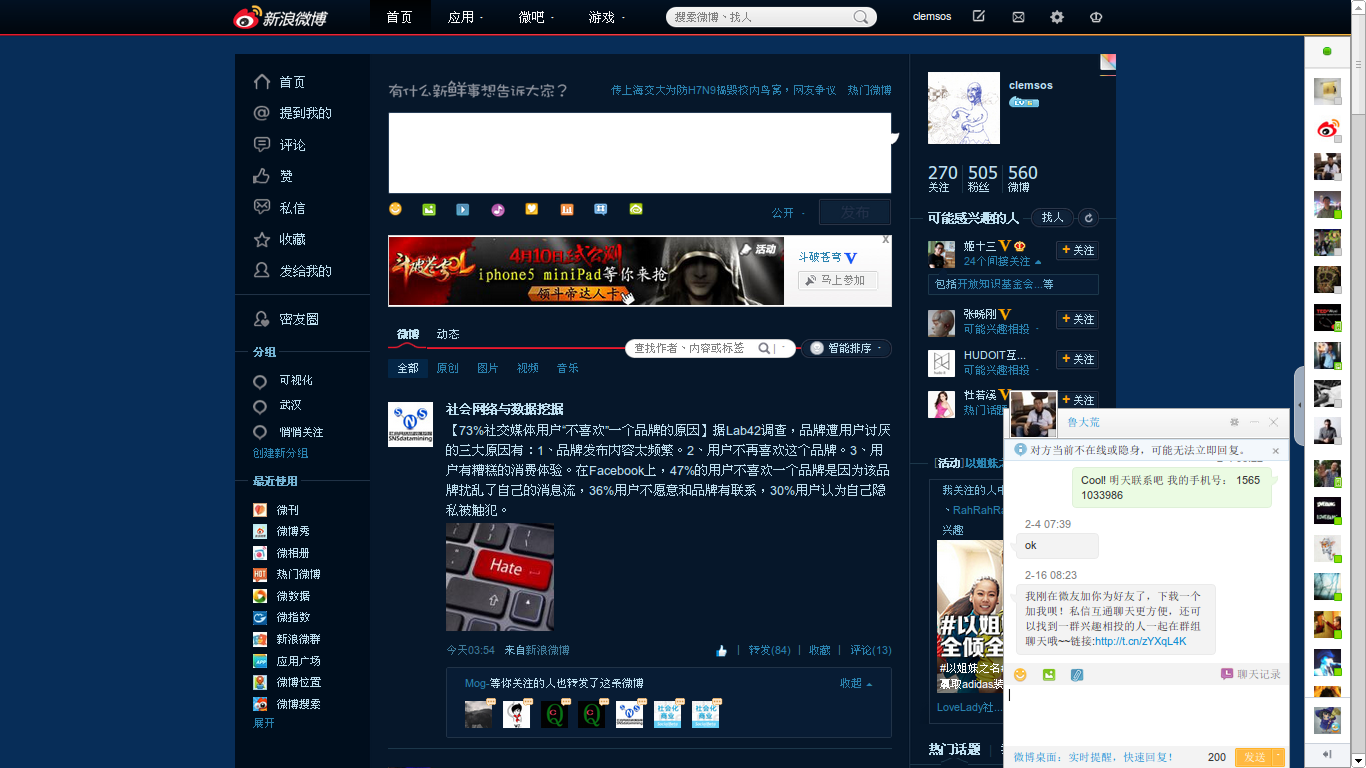
\includegraphics[scale=0.3]{figures/chap1/screenshot.png}
    \caption[Capture d’écran de Sina Weibo]{Capture d’écran de Sina Weibo, réalisé le 9 Avril 2013 à 08:59}
    \label{fig:screenshot_weibo}
\end{figure}

Figure historique de l’Internet chinois, \textit{SINA Corporation} est célèbre pour son portail \url{sina.net} et son immense plate-forme de blogs qui en font le fleuron des fournisseurs de contenus en ligne en Chine. Spécialisée dans ``l’infotainment'' (un mélange très tabloïd d’actualité et de news people), \textit{SINA} est la première compagnie nationale chinoise à avoir été listée au \textit{NASDAQ} dès Avril 2000. Avec son \textit{Weibo}, la firme réussit un coup de force commercial et prouve une fois encore combien la censure gouvernementale est bénéfique à l’industrie du web chinois. Néanmoins, la réussite de \textit{SINA} et de son service de microblog ne se fait pas sans connaître de nombreux ajustements parfois chaotiques. En effet, la stratégie agressive d’acquisition d’audience soutenant la croissance de \textit{Sina Weibo} offre pour garantie aux utilisateurs de pouvoir mieux s’informer et discuter plus facilement en ligne. Dès le début de l’année 2010, les suppressions de comptes utilisateurs et de messages non désirés commencent à se répandre dans le service. Les discussions politiques sont régulièrement effacées et \textit{Sina} se voit contraint de mettre en place un système de censure efficace sous la pression du gouvernement de Pékin. Néanmoins, afin de continuer à garantir la croissance du service, la firme de Pékin laisse une relative liberté aux utilisateurs en étant plutôt souple sur la surveillance des discussions et les actions prises. Des personnalités publiques ou journalistes devenues “weibo-stars” mobilisent régulièrement l’opinion publique autour de sujets d’actualité, attirant souvent des millions de lecteurs et de commentaires. Plusieurs scandales éclatent en ligne, mettant en cause des officiels et leur famille\footnote{Le fils d’un haut-cadre du Parti, arrêté ivre par la police après avoir renversé 5 personnes, annonce : \textit{”Mon père s’appelle Li Gang”} et se voit immédiatement libéré. Cette impunité provoquera un tollé chez les internautes \url{http://www.chinadaily.com.cn/china/2011-03/02/content_12099500.htm}}. Le 23 Juillet 2011, deux trains déraillent sur la ligne reliant Ningbo à Wenzhou inaugurée en fanfare quelques jours auparavant, faisant près de 40 morts et quelques 200 blessés. La colère gronde alors que le gouvernement tarde pendant plusieurs jours à prendre la parole sur ce sujet d’actualité épineux. Sur la toile et \textit{Sina Weibo} en particulier, les discussions vont bon train et les internautes indignés commentent le dernier drame du développement trop rapide de la Chine, où se mêlent détournement de fonds, corruption et sécurité publique. 


\begin{figure}[htbp]
    \centering
    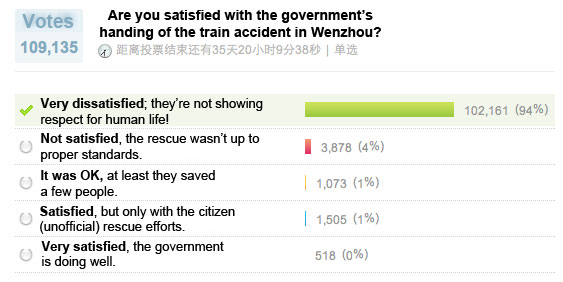
\includegraphics[scale=0.7]{figures/chap1/train.jpg}
    \caption[Sondage Weibo concernant l'accident de train de Wenzhou]{Un sondage publié sur \textit{Sina Weibo} (traduction C. Custer, Tech in Asia, 1er Aout 2011), consulté le 24 Février 2014, à 22h12.}
    \label{fig:poll_weibo}
\end{figure}

\textit{Sina Weibo} désactive alors la fonction de commentaires des messages. Dans les jours suivants, le gouvernement fait enfin une déclaration officielle sur les causes de l’accident de train puis se décide à agir en mettant en garde les internautes trop audacieux de représailles à venir. Les messages controversés sont supprimés, plusieurs comptes utilisateurs sont fermés, la police convoque les meneurs des discussions et d’autres mesures d’intimidation sont menées auprès des journalistes et des weibo-stars qui se seraient exprimées un peu trop directement à l’égard du Parti. Dans le même temps, le gouvernement a du mal à se saisir de ce nouvel outil. Alors que les administrations locales, universités et les médias d’État ont plutôt bien réussi le virage de leur stratégie de communication vers le microblog, les membres du gouvernement de Pékin ouvrent des comptes où ils sont parfois raillés, tournés en ridicule et harassés de questions. En Février 2012, les quatre plus grosses sociétés de microblog (dont \textit{Sina Weibo}) annoncent que chaque utilisateur est maintenant contraint de modifier son profil pour mentionner son véritable nom, prénom ainsi que son numéro de carte d’identité. Cette velléité de vérification échoue et est abandonnée quelques semaines plus tard face à la mobilisation des utilisateurs et la difficulté de faire appliquer de telles mesures. Le gouvernement de Pékin édite pourtant une série de règles \textit{“Several Regulations on Microblog Development and Administration Enacted by the Beijing Government”} dont la plus notable sera la possibilité de condamner tous ceux qui auront participé à la diffusion d’informations considérées comme fausses, erronées ou mensongères. Face à la multiplication des actions gouvernementales et à l’apparition d’autres plate-formes, la croissance du nombre d’utilisateurs de \textit{Sina Weibo} est désormais stoppée pour aborder une phase de déclin estimé à près de 10\% dans les deux premiers mois de 2014\footnote{D’après le CNNIC cité dans l’article  \textit{“China’s Twitter is bleeding users”}, 17 Janvier 2014, \url{http://blogs.marketwatch.com/thetell/2014/01/17/chinas-twitter-is-bleeding-users}, consulté le 17 Février 2014 à 18:17}. 

\begin{figure}[htbp]
    \centering
    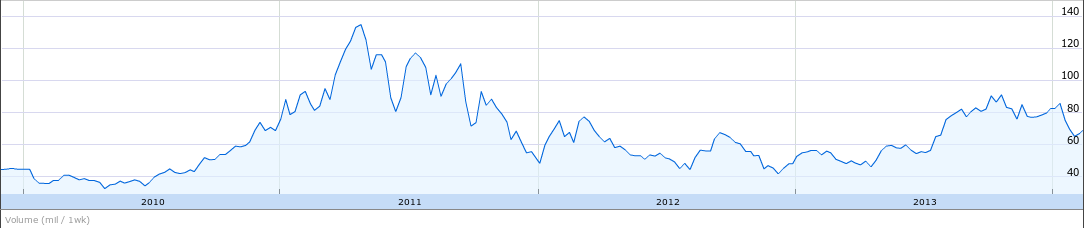
\includegraphics[scale=0.4]{figures/chap1/sina.png}
    \caption[Cours de l’action SINA au Nasdaq entre 2009 et Février 2014]{Cours de l’action \textit{SINA} au Nasdaq entre 2009 et Février 2014 - Source : \textit{Google Finance}, consulté le 17 Février 2014 à 15:28 }
    \label{fig:sina_nasdaq}
\end{figure}

A la lecture de l’histoire de \textit{Sina Weibo} on constate l’ambivalence des actions officielles du gouvernement chinois dans la réussite économique des entreprises d’Internet. Si la firme \textit{SINA} a bénéficié de prime abord d’un avantage compétitif notoire par l’élimination de la concurrence, elle a par la suite souffert des conséquences du contrôle politique de l’Internet, avec notamment une perte de ses utilisateurs.


\subsection[Sina Weibo, un usage plus ludique que \textit{Twitter} ]{Sina Weibo, un usage plus ludique que \textit{Twitter} }

Dans son article nommé \textit{A Tale of two microblogs}, Jon L. \cite{Sullivan2012} raconte comment l’événement historique de la fermeture de \textit{Twitter} en Chine a vu la communautés des microbloggers chinois se scinder en plusieurs groupes distincts : 

\begin{itemize}
\item \textit{Twitter} rassemble une communauté avide de libres discussions, souvent très politisées voire radicalement en opposition avec le gouvernement chinois.
\item \textit{Tencent Weibo} est utilisé par les utilisateurs de \textit{QQ}, typiquement des personnes aux revenus plus faibles accédant au web depuis leurs mobiles.
\item \textit{Sina Weibo} est le favori des travailleurs urbains, souvent plus jeunes ou éduqués, représentant davantage la classe moyenne montante.
\end{itemize}

Dans la littérature en sciences informatiques, plusieurs articles proposent des comparaisons entre \textit{Twitter} et \textit{Sina Weibo}. Une large analyse quantitative et comparative menée avec des jeux de données des deux services \citep{Gao2012} nous apprend que le contenu de \textit{Sina Weibo} est davantage corrélé avec des sentiments positifs (analysés automatiquement). Les utilisateurs de \textit{Sina Weibo} parlent davantage de lieux et de personnes alors que les utilisateurs actifs sur \textit{Twitter} s’intéressent plus aux organisations. Également, \textit{Sina Weibo} connaît un pic d’activité le week-end alors que \textit{Twitter} affiche généralement une baisse de régime dans les fins de semaine. Ces différentes indications suggèrent que \textit{Sina Weibo} serait davantage utilisé pour des activités de loisir quand \textit{Twitter} se destinerait à un usage plus professionnel. Une étude s’intéressant aux tendances sur \textit{Sina Weibo} \citep{Yu2011} indique que la majorité des comptes les plus influents de \textit{Twitter} ont été vérifiés contrairement à \textit{Weibo} où le taux est plus faible chez les grands utilisateurs. La vérification d’un compte se fait par l’authentification auprès du fournisseur de service afin d’attester l'identité de la personne utilisant le compte. C’est un enjeu important pour les figures publiques (marques, stars, hommes politiques, etc.) Cet indicateur nous montre donc l’intérêt professionnel fort entourant \textit{Twitter}, moins pressant dans le cas de \textit{Sina Weibo} où moins de personnes ont ressenti la nécessité de faire officialiser leurs comptes. Sur les deux services de microblog, les utilisateurs inscrits possèdent un réseau de relations identifiables par leur souscription aux fils d’infos d’autres utilisateurs (\textit{follow}). La relation peut être inexistante (\textit{none}), mutuelle (\textit{friend}) ou unidirectionnelle (\textit{follow}, un utilisateur suit un autre mais n’est pas suivi par ce dernier). La comparaison d’échantillons des graphes sociaux issus des deux services \citep{Chen2012} montre comment les relations sur \textit{Sina Weibo} sont plus dissymétriques et moins réciproques, reflétant une hiérarchie plus forte entre les utilisateurs que \textit{Twitter}. 

Un autre facteur important de différentiation entre les deux services est la nature de la diffusion des contenus postés sur \textit{Sina Weibo}. Contrairement à \textit{Twitter} où le texte domine, la majorité des posts de Weibo contiennent des images ou des vidéos \citep{Zhao2012}. Les posts possédant des contenus multimédia (images, vidéos...) sont plus susceptibles d’être diffusés largement et restent en moyenne actifs pour une durée plus longue \citep{Zhao2012}. Également, les contenus sur \textit{Sina Weibo} possèdent une proportion moins élevée de retweets et de commentaires que sur \textit{Twitter} \citep{Zhao2012, Gao2012}. L’activité de la population de \textit{Twitter} est plus intense, moins tournée vers la diffusion de masse et plus réactive aux influx de nouveaux contenus. 

Nous voyons donc que le paysage de \textit{Sina Weibo} se constitue autour de stars et célébrités concentrant l’attention avec des contenus à la diffusion très large. Moins tourné vers l’actualité et la conversation que son homologue \textit{Twitter}, \textit{Sina Weibo} agit comme véhicule de contenus à grande audience, souvent publiés par des personnalités publiques célèbres. Des études quantitatives montrent bien que les contenus les plus échangés et discutés concernent les loisirs et divertissements, la mode, la santé, etc. \citep{Li2013}. Les messages à caractère humoristique (texte, images et vidéos) occupent également une place prépondérante dans les échanges des utilisateurs, contrairement à son homologue américain \textit{Twitter} dominé plutôt par les sujets d’actualité \citep{Yu2011}. \textit{Sina} poursuit ainsi son rôle historique de leader chinois de \textit{l’infotainment}. 

Pourtant, la population de jeunes urbains qui soutient la croissance de son service de microblog reflète aussi les transformations en cours dans la société chinoise. Les journalistes et spécialistes de l’information sont les premiers à se saisir de ce nouveau média. Dans un discours à Stanford en 2013, le PDG de \textit{Sina} Charles Chao explique : 

\begin{quote}
\textit{Le plus grand changement apporté par le microblog en Chine concerne d’abord l’industrie des médias elle-même. Aujourd’hui, plus de 30\% des actualités ont d’abord été reportées sur \textit{Sina Weibo} avant d’atteindre les médias   traditionnels. Le rôle des médias traditionnels a été déplacé vers un traitement des informations en profondeur (in-depth reporting).} \footnote {Charles Chao, PDG de Sina pendant la Stanford Graduate School of Business China 2.0 tenue le 3 Octobre 2013. Disponible en vidéo \url{http://www.youtube.com/watch?v=tlliivJKHk8}, consultée le 19 Février 2014 à 11:23} (traduction de l’auteur)
\end{quote}

L’omniprésence des supports mobiles (smartphones, tablettes)\footnote{Selon l’Universal Telecommunication Union, \textit{``la Chine dépasse 1 milliard d’abonnements mobile, avec 400 millions d’utilisateurs d’Internet mobile dépasse ainsi les États-Unis comme leader du marché des smartphones''}, \url{http://mobithinking.com/blog/china-top-mobile-market} consulté le 24 Février 2012.} permet en effet des modes de traitement de l’information jusqu’ici inconnus qui bousculent les hiérarchies très contrôlées des salles de rédaction chinoises. Alors que la population urbaine croît rapidement, le smartphone est \textit{``the first big urban purchase''} \citep{Wallis2013} pour les nouveaux arrivants en ville et représente un outil indispensable de participation à la société. En 2008, la Chine était le seul pays en Asie où les moins de 30 ans possèdent plus d’amis en ligne que hors ligne \citep{Hinckley2009}. Ainsi, les réseaux sociaux jouent un rôle primordial dans la socialisation urbaine et viennent changer les modes d’expression. Le lectorat chinois a perdu toute confiance dans la plupart des médias traditionnels suite à l’absence répétée de courage et à la rétention d’informations cruciales dans les dossiers importants animant le pays. 

Le microblog s’installe comme une nouvelle source de confiance pour des millions de citoyens voulant comprendre et prendre part aux changements cruciaux de la société chinoise moderne. Un rapport de l’Institut de Journalisme Reuters à l’Université Oxford paru en 2013 montre comment les usages du microblog ont amené des transformations dans le quotidien des journalistes chinois. Le journalisme d’investigation a notamment connu un essor important grâce au renouvellement des sources et une large diffusion en ligne des sujets. \textit{Sina Weibo} n’a pas amélioré nécessairement la qualité de leurs investigations, mais a par contre permis une plus grande dissémination. Il est à noter que les spécificités de l’écriture chinoise rendent possible l’écriture d’un court texte en 140 caractères, alors qu’une telle longueur autorise seulement une courte phrase dans une écriture utilisant un alphabet latin. La mobilisation des utilisateurs pour la protection des journalistes a également joué un rôle important ainsi que le renforcement de procédés de vérification existant depuis longtemps sur les forums du web chinois. Très populaire dans les années 2000, Le \textit{``moteur de recherche de viande humaine''} (\textit{renrou sousuo}) est une forme de traque d’individus en ligne réalisée par un large nombre d’internautes à partir d’un nom ou d’une photo. Il s’agit souvent de retrouver quelqu’un désigné comme ``coupable'' (d’adultère, de corruption, etc) en réunissant un maximum d’informations à travers la Toile afin d’identifier ou de localiser la personne. Devant les dérapages rapides de ce type de procédés, les questions d’éthique sont au cœur des discussions qui entourent le journalisme en ligne. En effet, l’usage des médias sociaux a permis à certains journalistes de faire pression sur les pouvoirs publics, amenant parfois à la censure de leurs travaux, mais a également permis une très large auto-promotion pour de nombreux journalistes devenus des stars de \textit{Weibo}.

\begin{figure}[htbp]
    \centering
    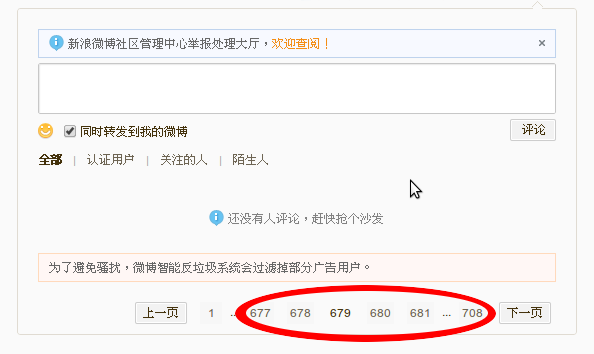
\includegraphics[scale=0.5]{figures/chap1/comments.png}
    \caption[Commentaires supprimés par Sina]{La trace des commentaires supprimés par Sina est encore visible - Page 677 à 708, les commentaires ont été supprimées, soit approximativement 4\% messages supprimés (589 messages sur 13452, à raison de 18 à 20 messages par page). Capture d’écran effectuée le 29 Janvier 2013 à 12:32:42, \url{http://www.weibo.com/1701401324/zeoBquVKi}, consulté le 16/02/2013.}
    \label{fig:comments}
\end{figure}

Le contrôle des contenus sur \textit{Weibo} est donc une réalité quotidienne et a été depuis son lancement la source de plusieurs études. Les formes les plus courantes sont : la suppression de posts, la suppression de comptes utilisateurs et le blocage de mots-clés. Le blocage de mots-clés s’effectue dans le moteur de recherche interne du site (“pas de résultats” quand vous cherchez un mot bloqué) et plus récemment par l’impossibilité de poster un message contenant des mots ou des adresses web bloqués \citep{Ng2013}. La pratique de la suppression de comptes s’est intensifiée en 2013\footnote{ \textit{“Over 100,000 \textit{Sina Weibo} Accounts Shut Down or Penalized for Govt Rules Violations”} par Gabriela Vatu, 14 November 2013 \url{http://news.softpedia.com/news/Over-100-000-Sina-Weibo-Accounts-Shut-Down-or-Penalized-for-Govt-Rules-Violations-400289.shtml} consulté le 17 Février à 16:42} avec notamment la suppression de millions de “zombies” présents sur le site. Les “zombies” sont des comptes utilisateurs créés par des robots dans le but de reposter automatiquement des contenus et d'augmenter le trafic sur le site. Les exigences des annonceurs publicitaires de plus en plus présents sur le site ont obligé \textit{Sina Weibo} à faire la chasse aux robots sur son site, faisant ainsi diminuer le nombre de comptes actifs de manière significative. La firme Sina est garante auprès du Ministère de la Sécurité Publique chinois des contenus qu’elle diffuse et effectue à ce titre une surveillance constante pour supprimer les messages “non-conformes”. Lors de nos recherches, nous avons constaté que l’interface de \textit{Sina Weibo} garde la trace des commentaires supprimés par le système d’administration. Dans les messages supprimés se trouvent à la fois des posts d’utilisateurs “zombies” et les posts jugés incorrects par les administrateurs. Au total, la suppression des messages s’effectue avec un taux estimé à environ 16\%, allant jusqu’à plus de 50\% dans certaines provinces comme Ningxia ou le Tibet contre seulement 12\% à Beijing \citep{Bamman2012}.


\section[Code, langage et milieu(x) numérique(s)]{ Code, langage et milieu(x) numérique(s)}

L’espace d’expression offert par l’Internet chinois et ses services de réseaux sociaux héberge donc une variété de pratiques, de questions et de réflexions qui nécessitent d’être appréhendées avec des outils de problématisation et d’analyse spécifiques. Dans la troisième et dernière partie de ce chapitre introductif, nous allons donc nous pencher sur les concepts existants dans la littérature scientifique sur l’existence \textit{in situ} des objets numériques. Afin de mettre en perspective le Web chinois et l’histoire de ces objets, nous introduirons notamment le concept de \textit{milieu numérique}, héritier de l’idée complexe de milieu que nous explorons ci-après.

\subsection[Lieu, espace, territoire et technologies]{Lieu, espace, territoire et technologies}
Géographie, management et diffusion de l’innovation, histoire des technologies, \textit{cultural studies} ou études “nationales”, les travaux qui s’intéressent aux relations entre technologies, espace, lieux et territoires sont nombreux et offrent un paysage riche où se croisent de nombreuses disciplines scientifiques. L’influence des réseaux de transports sur l’expérience humaine et le développement des villes a notamment été largement étudiée \citep{Offner1993,Doulet2001}. L’Internet a également fait l’objet de nombreuses études monographique (par pays) ou comparative, une étude à l’échelle mondiale présentant en effet des problèmes de données et évidemment d’échelle \citep{Dupuy2004}. En Chine où l'urbanisation produit actuellement une vaste migration des ruraux vers la ville, l'utilisation des réseaux sociaux médiatise bien souvent les choix de lieux et les rencontres des nouveaux arrivants. De nombreux groupes de discussions réunissent par exemple les nouveaux acheteurs d’immobilier qui échangent leurs stratégies d’achat et de défense de leurs droits et de leurs biens \citep{Li2013}. L’usage des réseaux sociaux revêt pour les nouveaux arrivants une importance capitale, notamment dans la recherche de groupes similaires et l’échange d’expériences. A travers le navigateur, ils s'approprient la ville étrangère pour s'en construire peu à peu une représentation à leur image.

La carte notamment joue sur le web un rôle important d’abord en tant qu’illustration, puis plus récemment d’interface avec le réel. Loin d’être figée par le territoire, la carte le décrit sous un ou des angles particuliers \citep{Brunet1987, Jacob1992}. Le développement de standards comme le système GPS \citep{Haklay2008} et de services et outils de cartographie ont contribué à une appropriation de la pratique cartographique par un nombre croissant de personnes \citep{Crampton2009}. De nouvelles formes de données produites par les utilisateurs parfois appelées \textit{``volunteered geographic information''} \citep{Elwood2008} utilisent les services en ligne comme Google Maps pour dessiner un \textit{``miroir du monde offline''} \citep{Graham2011}. Le courant dit de la néogéographie fait usage du GIS et des outils en ligne (Google Maps, Flickr, etc.) pour comprendre les pratiques de ces nouvelles formes de \textit{``géographies volontaires''} \citep{Turner2006}. Ce rôle croissant de la cartographie dans l’usage d’Internet produit un \textit{``Geoweb''} constitué de données et métadonnées spatiales \citep{Crampton2009}. Le point d'entrée unique qu'offre le marqueur spatial (\textit{geotag}) réunit souvent de vastes quantités de données disparates: Open Data territorial, géo-localisation, GIS, POI\footnote{GIS : Geographic Information System ; POI : Point-Of-Interest}, etc. \citep{Torrens2010}. Cette présence accrue dans le réseau dessine l’enjeu non seulement de cartographier le monde, mais également de cartographier le réseau lui-même, ouvrant ainsi de nouvelles voies pour découvrir la construction sociale des espaces par des pratiques individuelles et de groupe. Dans cette étude, nous avons donc choisi d’interroger les objets numériques afin de comprendre comment se structurent la parole et la conversation dans le contexte unique de l’Internet chinois. Afin d’articuler les multiples dimensions d’analyse qui viennent enrichir notre réflexion, il nous faut donc brosser un portrait en large de l’Internet chinois, en le considérant tour à tour comme un \textit{espace} structurant pour les actions des internautes qui le pratiquent, comme un \textit{territoire} sujet aux relations de pouvoir actualisées par les groupes et individus et enfin comme un \textit{lieu} habité par ceux qui y construisent chaque jour des significations communes. Nous proposons ici une revue sélective des quelques travaux à même de nous apporter des éclairages pertinents dans la vaste littérature s’intéressant aux dimensions géographiques des TIC.

\subsubsection[Code / space : l’espace transductif des TIC]{Code / space : l’espace transductif des TIC}

Dans leurs recherches autour de la géographie des technologies numériques, Dodge \& Kitchin ont travaillé à développer le concept de code comme un élément fondateur des espaces modernes dans lesquels nous évoluons. Reflétant l’importance croissante accordée aux TIC dans l’environnement urbain, ils citent un travail sur la production automatique des espaces : \textit{“De plus en plus, les espaces de la vie  quotidienne nous parviennent chargés de logiciels (software)”} \citep{Thrift2002} En effet, si le projet urbain a été guidé pendant le demi-siècle dernier par l’apparition de la technologie automobile dans l’espace des rues, les TIC paraissent prendre le relais avec l’idée d’une ville intelligente et connectée, connue sous le nom de \textit{`` smart city ''} \citep{Ascher2009,Picon2014}. Dodge \& Kitchin ont donc fait du \textit{code} une des pierres d’angles de l’appréhension de l’espace dans leur travail en le définissant comme suit : 

\begin{quote}
\textit{``an instruction or rule that has a single outcome determined by a binary logic (yes/no). The combination of these indidivuals logic rules produces code (program).''} \citep{Kitchin2011}.
\end{quote}

La part croissante des TIC dans nos espaces quotidiens amène les auteurs à envisager l’espace dans son interaction avec le code, symbolisant la suite d’instructions machiniques et électroniques qui permettent à un espace de remplir sa fonction. Dans un article intitulé \textit{Flying through code/space: the real virtuality of air travel}, Dodge \& Kitchin analysent la structure des espaces aéroportuaires. De l’achat des tickets jusqu’au vol des avions en passant par la gestion des bagages, le bon fonctionnement d’un aéroport est entièrement régi par les longues successions d’instructions du code. Ici, Dodge et Kitchin proposent le concept de code/space pour décrire ce type d’espace spécifique où lorsque le code échoue (\textit{failure}) alors le code/space tout entier échoue \citep{Dodge2004}. L’exemple de l’aéroport est parlant : si le système de check-in des bagages ou les machines responsables du contrôle de sécurité des passagers ne fonctionnent pas, alors l’espace aéroportuaire ne peut exister en tant qu’aéroport. L’analyse de la spatialité ne se situe alors plus dans un domaine sémantique ou narratif, mais plutôt dans les processus et opérations qui s’y déroulent et le code et les technologies y jouent un rôle primordial : 

\begin{quote}
    \textit{``Code is employed as the solution to a problem, a particular kind of transduction  is occurring.''} \citep{Kitchin2011}. 
\end{quote}

L’espace n’est pas un donné mais s’explique plutôt comme : \textit{``une forme d’ontogenèse (en perpétuel devenir-au-monde), l’espace est une pratique; un faire ; un événement (…) qui ne pré-existe pas à son faire (doing)''} \citep{Kitchin2011}. L’espace est considéré non pas comme une production, mais comme une \textit{transduction}. Reprenant le travail de Simondon sur l’individuation par la technologie, Dodge et Kitchin présentent l’espace comme une pratique qui comprend les actes, actions, occurrences, mémoires, perceptions, etc. d’un groupe d’individus s’y trouvant. La fonction de l’espace est structurée par les individus et le code y est considéré comme une entité agissante. Dans le \textit{code/space}, la relation dyadique entre code et espace est bijective: l’un ne peut aller sans l’autre. En terme simondonnien, la transduction ne peut être assurée sans code. Si l’exemple de l’aéroport illustre bien cette nécessité du code dans le devenir-espace, Dodge et Kitchin ont également identifié d’autres catégories où cette relation est plus ténue : les \textit{coded spaces}, qui peuvent poursuivre leurs fonctions même lorsque le code échoue ; les \textit{background coded spaces} où les processus de transduction induis par l’espace ne s’appuient pas nécessairement sur le code, mais proposent néanmoins des possibilités de l’activer (machine éteintes ou inactives, etc.) 

L’analyse fonctionnelle des rapports entre espace et technologie de Dodge \&Kitchin montre comment les TIC peuvent être un facteur \textit{transductif} pour les individus se mouvant dans les espaces de leurs vies quotidiennes. Si nous appuyons pleinement ce constat, il nous semble que le parti-pris des auteurs de considérer le “code” comme une abstraction incluant uniquement les instructions ou “logiques machiniques“ ferme la porte à l’immense densité des activités symboliques qui se jouent dans l’usage des technologies. Comment notamment considérer les “contenus” du web dans cette grille de lecture? Comment resituer dans une perspective historique les logiques de médiation de l’espace par les technologies de l’écriture? Il nous semble en effet que la faillite fonctionnelle (\textit{failure}) des code/space précède l’arrivée des technologies et s’opère déjà à un niveau symbolique - la fonction de l’espace du Palais du Louvre après la chute des rois de France se voit radicalement modifiée. La transduction opérée lors de la pratique d’un espace s’effectue dans un jeu d’appropriation symbolique qui passe notamment mais pas seulement par les technologies. Les technologies du langage et de l’information jouent notamment un rôle crucial dans l’affirmation du récit symbolique (\textit{narrative}) qui construit l’espace. L’activité du code dans la structuration des code/space de Dodge \&  Kitchin existe sous une forme non seulement fonctionnelle mais également sémantique, voire phatique ou même esthétique comme l’a décrite Jakobson dans ces analyses des fonctions du langage \citep{Jakobson1956}. Au-delà de sa dimension machinique, le code possède les caractéristiques d’une \textit{poiesis} dépassant l’idée simple de fonctionnalité pour exister dans la complexité d’une écriture comme traduction du langage humain et machine.

\subsubsection[Codes, discours et territoires des technologies]{Codes, discours et territoires des technologies}

Le code serait davantage à comprendre comme un mode d’expression humain à travers la technologie, actualisant l’\textit{épistémè} décrit par Foucault dans \textit{Les Mots et Les Choses} comme élément fondamental de la pensée d’une époque et sa considération pour le monde \citep{Foucault1996}. Ètat des connaissances scientifiques et littéraires, l'épistémè existe comme somme des savoirs d’une époque, présupposée traduite en un regard sur le monde. Le \textit{code} exprime les savoirs d’aujourd’hui dans de nombreux langages écrits. Le code source d’une page Internet, d’un programme informatique ou d’un driver hardware ne s’écrit pas seulement en langage ``machine'' mais fait appel à plusieurs langages informatiques et humains. A la fois production savante, outil scientifique, vecteur d’expression et interfaces des savoirs, le code constitue l’expérience narrative du monde par les TIC. Possédant de nombreux mots, aspects et syntaxes issus de multiples langues humaines, les replis de l’écriture informatique laissent transparaître de tout bord leur origine littéraire. L'alphabet se voit augmenté de nombreux caractères qui le rendent compatible avec l’encodage des bases de données - pensons à l’Unicode notamment \citep{Guichard2014}. Rappel à l'ordre, l'arrêt soudain de l’ordinateur ou la perte d’un fichier nous laisse frappés d’illettrisme. Seuls une minorité de personnes ``lettrées'' de l’informatique peuvent déchiffrer et comprendre le ``bug''. Ainsi, la définition du ``code'' de Dodge \&  Kitchin doit être étendue pour recouvrir plus largement les pratiques symboliques liées aux activités de l’écriture du code dans ces espaces.


Le code ainsi redéfini nous ramène alors à une lecture foucaldienne du discours dans sa relation intime avec le territoire \citep{Foucault2004}. Dans ces nombreux travaux sur la généalogie, Michel Foucault cherche à comprendre comment les relations de pouvoir créées par les discours portés sur les objets président à la production de territoires et d’interdits comme autant de sujets de ces discours. Nous définissons la \textit{discursivité} comme le processus de construction de ces discours. Historiquement, l’Internet a été très tôt sujet à l’appropriation par le discours de nombreux groupes actifs dans une volonté de territorialisation. La métaphore géographique et spatiale a structuré le vocabulaire de l’Internet dès sa création \citep{Graham1998}: site, cyberspace, etc. L’\textit{Electronic Frontier Foundation} se charge de protéger l’u-topie qu’est Internet avec sa fameuse \textit{Déclaration d’Indépendance du Cyberespace} \citep{Barlow2001}. A l’opposé du spectre, les autoroutes de l’information in-forment le paysage comme autant de géogrammes massifs \citep{Berque1999}. L’appropriation des protocoles du réseau, notamment par la lutte pour le respect de standards ouverts ou partagés, s’ancre également dans les pratiques du discours. Les mots \textit{free} et \textit{open} cristallisent l’histoire des revendication territoriales de l’Internet \citep{Blondeau2000}. L’autre grande métaphore constitutive de l’Internet est textuelle avec ses pages, langages et hypertextes \citep{Vandendorpe1999}. La formule choc \textit{``Code is law''} \citep{Lessig2006} résume l’idée  que les processus textuels du code mettent en jeu un ensemble de rôles, protocoles et mises en scène qui agissent comme autant d’autorités à travers le discours. La jurisprudence fait loi, comme écrit sur les murs des bureaux de \textit{Facebook} à Palo-Alto : \textit{``Code wins arguments''} \footnote{Dans la Lettres aux Investisseurs écrite par M. Zuckerberg  pour l’IPO de \textit{Facebook} \url{http://www.sec.gov/Archives/edgar/data/1326801/000119312512034517/d287954ds1.htm\#toc287954_10}}. La territorialisation de l’Internet se fait ainsi au travers d’un ensemble de pratiques discursives, méta-grammaire des discours en ligne. La confrontation symbolique au sein des territoires numériques se poursuit dans le discours, réifié dans les pratiques du code.

Sur l’Internet chinois, les pratiques de censure de l’écriture en sont le reflet le plus frappant. Blocage de mots-clés, détournements de langage, suppression et modification de texte sont l’expression de cet affrontement de discursivités parfois antagonistes. La Grande Muraille gouvernementale scanne les masses de texte pour reconnaître et stopper des mots tels que \textit{``Printemps arabe''} ou \textit{``évènements de Tian-An Men''} \citep{MacKinnon2012}. Néanmoins, l’état actuel des techniques de \textit{data mining} ne permet pas encore de déceler les phénomènes langagiers comme les jeux de mots ou l’ironie. Bien souvent, les internautes chinois choisissent l’humour pour permettre à leurs idées de se frayer un chemin. Revêtant leurs masques de chat, les internautes chinois sont devenus spécialistes dans la publication de jeux de mots, chansonnettes et petites vidéos d’animaux, comme autant de couperets cinglants pour railler les officiels trop pompeux de Pékin. Dans la guerre de l’information que se livrent sans cesse censeurs et internautes, de simples photos truquées de crabes et de lamas peuvent devenir héroïques. Ces blagues numériques, d’apparence inoffensive, font chaque jour le tour de la Toile chinoise, portant en elles toute la subversion d’internautes aspirant à plus de liberté. Début 2010, alors que pleuvaient les longs discours pieux du Parti sur l’harmonie de la nouvelle société (en chinois \textit{hexie}), on voit apparaître en ligne des essaims de crabes de rivière (se prononçant également \textit{hexie}) couverts de chaînes en or criant : \textit{“Vive l’harmonie”} au volant de leur limousine. Devenus aujourd’hui une image de la corruption des hauts dignitaires du Parti, on croise régulièrement dans les commentaires d’un article officiel un petit crabe de rivière, tel un rapide rappel posté par un lecteur.


\begin{figure}[htbp]
    \centering
    \subfloat[(hexie) : Harmonie / Discours du PCC sur l’harmonie]{ 
        
\includegraphics[scale=0.37]{figures/chap1/hexie2.jpg} 
    }
    \subfloat[(hexie) : Crabe de rivère / Mème satirique]{ 
        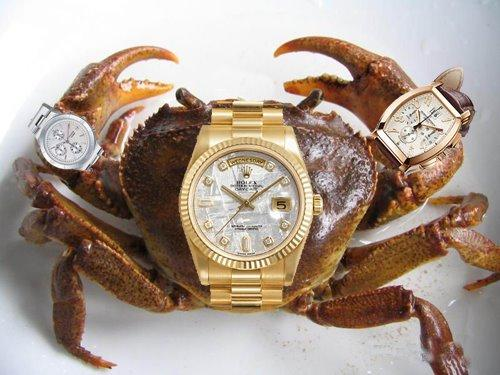
\includegraphics[scale=0.37]{figures/chap1/hexie.jpg} 
    }
    \caption[Hexie, les crabes de rivières]{ \zh{和谐} VS \zh{河蟹} - Mot de la semaine : Crabe de Rivière - China Digital Times du 21 Mars 2012 - Licence Creative Commons \url{http://chinadigitaltimes.net/2012/03/word-of-the-week-river-crab}, consulté le 15 Février 2013.}

\label{fig:hexie}
\end{figure}

On voit bien comment le code décrit un territoire sujet à l’autorité politique sous la forme d’un système de \textit{data mining} cherchant à mettre en forme le discours. La fonction du \textit{code/space} sémantique que forme ici l’espace de l’Internet est réécrit par un jeu de langage. La circulation d’objets digitaux permet de reterritorialiser cet espace en apparence régi par un code strict de censure. 

\subsubsection{Les lieux des technologies}
Dans son célèbre livre sur les Arts de Faire, \cite{Certeau1980} considère la ville comme un texte dont chaque piéton énonce et révèle (\textit{performe}) des sens nouveaux par son activité de marcheur. Actualisant l’espace urbain par sa marche, l’habitant de la ville s’approprie des lieux restant néanmoins partagés avec d’autres. Au détour des rues, le sens commun des lieux urbains se construit avec les multiples énonciations de ceux qui les habitent et les font vivre. Cette magnifique image de la poésie du texte urbain met en lumière la dualité que nous avons abordée précédemment : l’espace ne peut fonctionner sans les pratiques de ses habitants. Plus encore, l’être-ensemble et le devenir-soi procèdent de la construction de lieux communs, \textit{poiesis} des espaces habités. Les TIC font aujourd’hui souvent partie intégrante des lieux que nous habitons. \cite{Graham1998} dans son travail sur l’étude des lieux et de leur rapport à la technologie identifie trois types majeurs d’approches dans la littérature :


\begin{enumerate}

\item L’approche \textit{``substitutive''} ou \textit{``transductive''} qui voit dans l’arrivée des TIC la disparition de la valeur des lieux : un idéal de proximité utopique \citep{McLuhan1962} ou un discours dystopique sur leur proche disparition \citep{Virilio1998, Auge1995}. Ces considérations sont les formes traditionnelles du débat accompagnant l’innovation dont sont férus la communication industrielle et la critique des médias \citep{Ramonet2001}, restant souvent purement prospectif et faisant peu de cas des usages.

\item Plus modérée, l’approche qualifiée par Graham de \textit{``co-évolutionniste''} s’interroge sur la façon dont les interactions dynamiques des espaces virtuels (\textit{space of flows}) et réels (\textit{space of places}) \citep{Castells2009} produisent de nouveaux lieux . Ces études économiques et sociales prennent la forme d’une médiologie de l’espace adaptée aux études stratégiques pour l’urbanisme et l’implantation des télécommunications. Son interprétation par les aménageurs lui donne parfois une dimension déterministe peu utile à la compréhension des phénomènes liés à l’appropriation et l’historicité des technologies \citep{Offner1993}.

\item Une dernière approche plus récente se cristallise autour de l’idée de relations et de réseaux. Afin d’éviter l’écueil des causalités directes et de la notion fataliste d’impact, les lieux sont présentés comme \textit{`` des moments articulés dans un réseau de sens et de relation sociales ''} \citep{Massey1993}, des assemblages entre objets matériels “actants” \citep{Latour1996}, individus et groupes sociaux. Cette approche s’intéresse davantage au lieu comme une géométrie sociale en mouvement, liée au temps et à la situation \citep{May2001} et refuse l’idée d’une existence “virtuelle” commune à différents objets \citep{Bingham1996}.

\end{enumerate}

En privilégiant une approche dynamique et relationnelle des lieux comme constructions sociales de sens \citep{Kyle2007}, la technologie perd son rôle déterministe de productrice d’espaces et d’usages pour devenir une actualisation d’un espace-temps géographique et historique par des groupes d’individus. Comme le note Cresswell dans son travail sur les lieux : \textit{“places are practiced. People do things in place.”} \citep{Cresswell2004}. Il propose trois aspects pour décrire l’actualisation des lieux par leurs pratiques : location (un point dans l’espace, \textit{“the ‘where’ of place”}), \textit{locale} (les aspects visibles et tangibles du lieu, \textit{“the way a place looks”}) et \textit{sense} (\textit{“the feelings and emotions a place evokes”}). Néanmoins, cette définition ne permet pas d’appréhender l’existence des lieux en ligne (le site web d’un lieu est-il une \textit{locale} ou une partie du \textit{sense}?). Graham et Zook propose le concept de DigiPlace : \textit{`` DigiPlace - that is, the use of information ranked and mapped in cyberspace to navigate and understand physical places (…) In other words, DigiPlace represents the simultaneous interaction with software (information) and `hard-where' (place) by an individual.''} \citep{Zook2007}. S’inspirant des travaux de Harley sur le pouvoir du cartographe, leur travail sur le rôle de Google Maps dans la présence des lieux sur Internet met à jour l’interaction et l’hybridation entre existence spatiale et existence en ligne constituant les DigiPlace. 

Les phénomènes de transduction à l’œuvre dans les pratiques spatiales de l’Internet sont donc le reflet des états du réseau à un moment donné. Les lieux eux-mêmes forment ainsi un réseau basé sur leurs relations et similarités. Brunet dans son \textit{Vocabulaire de la Géographie} propose notamment l’idée de synapses: \textit{``espaces ou lieux par lesquels on passe, par où l'on communique, les isthmes, les détroits, les estuaires, les carrefours, les ports et les ponts, etc.;''} \citep{Brunet1972}. Envisagés par leur fonction ``synaptique'' , les lieux deviennent alors un construit social au rôle clair, évitant l’écueil d’une qualification en-soi. Aéroports, hypermarchés, aires d’autoroutes ou zones industrielles ont été qualifiés de \textit{non-lieux} par Marc Augé, produits d’une  hyper-modernité \textit{`` qui ne peut se définir ni comme identitaire, ni comme relationnel, ni comme historique. ''} \citep{Auge1995}. Réfutée plus tard par l’auteur lui-même, cette idée de lieux simplement \textit{produits}, et non construits fait l’impasse sur la tension d’usage, le devenir lieu que modèlent ses utilisateurs assidus ou épisodiques, ceux qui y travaillent voire même y habitent. Le lieu n’est pas nécessairement “patrimonial” comme produit d’une histoire, mais peut \textit{`` être ou ne pas être un non-lieu selon le statut de l'individu envisagé. ''} \citep{Debarbieux1993}. Les hypermarchés et leurs galeries marchandes sont des haut-lieux de socialisation et de rencontres pour les adolescents vivant en banlieue \citep{Matthews2000} mais paraissent froids et inhumains aux habitants des rues du centre-ville.

L’étude menée par Puel, Pons et Xiaoting autour des pratiques sociales environnantes les cafés Starbucks de Beijng (Chine) montre également comment la stratégie marketing de la firme s’appuie précisément sur cette “absence patrimoniale” pour faire sa place au travers du vaste territoire chinois. La non-existence d’un \textit{“bon café avec Internet”} dans les villes chinoises offre la possibilité aux usagers de ces cafés récemment apparus de s’y rendre pour utiliser l’Internet ou retrouver leurs amis \citep{Puel2007}. Ainsi, l’absence d’histoire n’interdit pas la constitution de pratiques communes à forte valeur symbolique se comprenant ici dans des réseaux d’appartenances mondiaux (jeune, dynamique, urbain, etc.). Dans son livre \textit{The Great, Good Place}, Ray Olenburg propose le concept de tiers-lieu pour décrire ces lieux qui, séparés de l’environnement de travail ou de la maison, permettent de se socialiser. Jouant un rôle majeur dans la construction de communautés et la constitution d’une société civile, ces tiers-lieu doivent répondre à certains critères comme: un cout d’accès nul ou modeste, une très bon accessibilité, la présence régulière des \textit{``habitués''}, un lieu accueillant et confortable et enfin un lieu où l’on peut rencontrer facilement de nouvelles personnes \citep{Oldenburg1999}. Ces tiers-lieux forment donc avant tout un réseau de lieux défini par les usages. L’idée de tiers-lieu virtuels a également été mentionnée pour désigner les chatrooms ou les plate-formes de réseaux sociaux en ligne remplissant des fonctions sociales similaires \citep{Soukup2006}.

Nous voyons donc qu’en considèrent les lieux de l’Internet, nous mettons à jour un ensemble de pratiques ne s’intéressant plus nécessairement à l’ordre du discours (et aux pratiques de censure notamment) mais plutôt aux phénomènes d’individuation, notamment au travers des multiples actes d’énonciation qui forment les pratiques et usages du web. Dans cette étude nous cherchons donc à comprendre de manière plus profonde comment les internautes habitent leur Internet. Il ne s’agit pas d’analyser le discours en termes de relations de pouvoir mais plutôt d’essayer de distinguer comment les circulations des objets numériques structurent les pratiques des internautes, comme autant de lieux habités quotidiennement.

\subsection[Le milieu : richesse et désuétude ]{Le milieu : richesse et désuétude }

Afin de problématiser les relations entre protocoles du discours et pratiques locales d’appropriation, nous avons choisi d’introduire le concept de \textit{milieu numérique}. Nous définirons d’abord brièvement ce concept avant de présenter un regard historique sur l’idée de milieu en science. Nous discuterons ensuite de l’acception particulière que nous avons choisie de défendre ici et nous verrons comment cette notion sera utile pour la suite de notre étude sur les réseaux sociaux en Chine.

L’idée de milieu numérique est a priori définie dans les termes suivants:

\begin{quote}
    \textit{``The multiple networks, which are connected by protocols and standards, constitute what I call a digital milieu.''} \citep{Hui2012}
\end{quote}

L’usage de multiples interfaces et le dédale des réseaux TIC constituent \textit{``un nouveau milieu perceptif''} \citep{Barboza2006}. Notre milieu physique est aujourd’hui (déc)ouvert par l’existence de notre milieu digital qui nous aiguille. Rencontres, restaurants et voyages sont souvent d'abord médiatisés par l’Internet. Ainsi, nous évoluons dans un milieu numérique agissant comme support de processus de transduction et de connaissance du monde. Le code prend ici pleinement part à la construction de ce milieu digital, à la fois déterminant pour la production des actes de discours et ouvert à l’appropriation des pratiques et usages du quotidien.

Historiquement, le concept de milieu se détache du centre pour resituer et mettre en perspective la relation des êtres à leurs environnements sous des jours parfois contradictoires. Débattue puis écartée mais toujours très usitée, la notion de milieu introduit autant le déterminisme d’un combat pour la survie et l’adaptation, que la liberté créatrice du sujet dans un univers ouvert à sa volonté. 

Pour illustrer au mieux la fécondité philosophique de la notion de milieu, nous allons tout d’abord essayer de comprendre la trajectoire de ce mot durant les siècles derniers \citep{Canguilhem1965}. Sans remonter à son aube étymologique, nous nous apercevons que le mot milieu décrit un trajet singulier dans le monde des sciences. Employé dès le XVIème siècle par Descartes dans son \textit{Traité de la lumière}, il représente pour Newton une mesure de distance dans l’éther, cette non-matière  structurant la gravitation qui fait se mouvoir les objets. Défini plus tard par d'Alembert dans son encyclopédie comme un : \textit{"espace naturel dans lequel un corps est placé, qu'il se meuve ou non"}, le mot connaîtra durant tout le XIXème un large développement sémantique en s'étendant de la physique à la biologie. Les naturalistes français de l’époque affirment que le milieu n’est pas seulement \textit{environnant} mais influe sur les êtres vivants. Ainsi Lamarck dès 1809 écrira dans sa \textit{Philosophie Zoologique}: \textit{"le milieu a une grande puissance pour modifier les organes"}. 

Le XIXème siècle est un moment marquant pour ce concept et structurant pour l’histoire des sciences dans son ensemble \citep{Taylan2010}. Auguste Comte, inspiré de la biologie, articule le vital au social dans la sociologie naissante et décrit le milieu comme \textit{``l’ensemble des circonstances extérieures (…) nécessaires à l’existence de chaque organisme déterminé''} \citep{Comte1838}. Comte introduit une première dialectique des rapports avec le milieu comme conditions de possibilité de la vie: \textit{``Tout être vivant (…) modifie sans cesse son milieu.''}, écrit-t-il alors. Le concept connaît un succès croissant en France et les penseurs d’Outre-Rhin se le réapproprient en lui donnent un sens différent. S’opposant au francisé \textit{Der Milieu}, le géographe Ratzel introduit dans son \textit{Anthropogéographie} (1899) le terme \textit{Umwelt}. Ce mot se démarque rapidement par sa dimension fortement déterministe. Dans un même mouvement, le physiologiste et biologiste Jakob von Uexküll étudie dans son laboratoire la tique et se rend compte que le milieu de la tique se définit non pas par tout l’environnement qui l’entoure mais seulement par ce qui lui est utile et approprié. Le milieu devenu \textit{Umwelt} s’oppose alors à l’environnement indifférencié et devient l’ensemble des éléments porteurs de significations (\textit{Merkmalträger}) pour un être. Uexküll propose ainsi une \textit{``biologie subjective''} étudiant les relations de chaque espèce avec son milieu. Dans l’Allemagne du siècle débutant, Uexküll diffuse largement sa théorie qui ne s’adresse pas tant aux animaux qu’à l’humain dont le milieu serai la Patrie (\textit{Heimat}) \citep{Feuerhahn2009}. Reflétant les débats guerriers entre la \textit{Kultur} allemande et la \textit{Civilisation} française \citep{Elias1975}, l’idée de Milieu cristallise la tension politique sur les relations entre nature et vivant qui déchirera l’Europe pendant longtemps encore. Foucault dans son cours au Collège de France du 11 Janvier 1978 parle de l’influence de l’idée de milieu sur la conception du territoire pour les urbanistes du XVIIIème siècle. Sous Louis XIV, les villes sont encore construites dans un espace conçu comme vide (voir \textit{Richelieu} en Indre-et-Loire). A l'inverse, la question de l’urbaniste du XVIIIème est de comprendre la ville dans son évolution future. L’enjeu est devenu l’\textit{adaptation} du milieu existant (à la fois urbain et naturel), la transformation du \textit{donné} compris comme un élément qu’on peut venir modifier. L’idée sous-jacente de milieu ouvre la possibilité de l’appropriation de la nature. En terme foucaldien, cette nouvelle bio-politique se fonde sur la territorialisation du milieu comme nouveau centre des enjeux de pouvoir. L’ère industrielle réalise ce projet d’une adaptation à la fois \textit{au} et \textit{du} milieu vu comme tension nécessaire de l’évolution, passage obligé vers la civilisation. Alors que l’humain est placé dans son rôle central par l’astronomie galiléenne puis l’évolution darwinienne, l’idée de milieu pose comme enjeu majeur du vivant la maîtrise de l’environnement - la lutte pour ne pas être maîtrisé. Poursuivi par la psychanalyse de Freud qui introduit l’Autre au sein du sujet, l’entreprise de décentrement de l’humain vers son milieu se joue dès l’abord dans les termes de la vie ou de la mort. Plus tard, Lacan identifiera la transition de la petite enfance à l’enfance par le ``stade du miroir'' comme moment où l’enfant différencie enfin le Milieu (\textit{Umwelt}) du Soi (\textit{InnenWelt}) \citep{Lacan2001}. Ce ``passage au milieu'' est donc d’une importance capitale puisque s’y joue la constitution de l’être dans la pensée de l'époque.

L’approche du milieu comme élément unificateur des sciences est un sujet toujours en discussion. L’introduction du concept d’\textit{environnement} a largement recentré le milieu sur le rôle déterminant de l’Homme avec  la théorie écologique \citep{Gandolfo2008}. Les conséquences de ce passage de l’idée de nature à celle de milieu restent profondes, notamment dans le droit civil où nous sommes passés d’un rapport du ``droit imposé'' de la nature au ``droit négocié'' du milieu \citep{Papaux2008}. Méta-réflexion, la discussion sur le ``milieu académique'' donne lieu à d’intéressants échanges \citep{Stengers2009} qui interrogent notamment la définition trop abrupte des disciplines scientifiques et leur herméticité. Parfois nommée \textit{mésologie}, l’étude du milieu se donne pour mission de réconcilier des pratiques diverses de la biologie à la sociologie en imaginant une étude par le milieu \citep{Stengers2003}. Source d'inspiration de la mésologie, les œuvres de Deleuze \& Guattari parlent déjà d’une philosophie du milieu : \textit{``Partir au milieu, par le milieu, entrer, sortir, non pas commencer ni finir, […] renverser l'ontologie, destituer le fondement, annuler fin et commencement.[…] C'est que le milieu n'est pas du tout une moyenne, c'est au contraire l'endroit où les choses prennent de la vitesse.''} \citep{Deleuze1972} 
La réflexion sur la technique et les technologies s’est notamment saisie à bras le corps de cette notion, avec notamment l’idée de \textit{milieu technique} par Friedman et Leroi-Grouhan \citep{Stiegler1998}. Tout geste (du plus banal au plus rare) s’effectuerait dans un milieu technique qui le rend possible. Gilbert Simondon dans son livre \textit{Du mode d’existence des objets techniques} continue cette réflexion avec ce qu’il appelle le milieu associé : 

\begin{quote}
    \textit{``médiateur de la relation entre les éléments techniques fabriqués et les éléments  naturels au sein desquels fonctionne l’être technique. (...) C’est ce milieu associé    qui est la condition d’existence de l’objet technique inventé.''} \citep{Simondon1989}. 
\end{quote}

Simondon problématise le milieu associé comme vecteur de l’\textit{individuation}, où se produit la rencontre entre objets et individus s'actualisant mutuellement. Poursuivant ce travail, Stiegler comprend les technologies de l’information comme un milieu essentiellement social, à la fois autour (environnement) et entre (medium) les individus \citep{Stiegler1998a}. Dans sa lecture critique des industries culturelles, Stiegler formule l’idée qu’un milieu est \textit{associatif} s’il permet l’individuation. A l’inverse, certains milieux seraient \textit{dissociatifs} car ils ne permettraient pas le devenir individu, à l’image des mass media qui divisent producteurs et consommateurs de symboles. La dynamique industrielle des deux derniers siècles a entraîné une massification des phénomènes culturels, créant un milieu technique considéré comme largement dissociatif car dé-réalisant pour les individualités \citep{Simondon1989}. Néanmoins, le renouveau technologique porté par l’apparition des technologies numériques ouvre aujourd’hui une page nouvelle pour l’individuation en offrant un milieu extrêmement associatif, fondé pour ainsi dire sur le lien. Voyant un nouvel âge des Lumières \citep{Stiegler2012}, Stiegler conçoit l’Internet comme un milieu qui ne serait pas structurellement dissociatif et pourrait donc recréer de nouvelles formes plus horizontales d’économie symbolique où existent davantage de symboles partagés. 

\subsection[Cyberespace et milieu numérique]{Cyberespace et milieu numérique}
\label{sec:cyber-milieu}

Associateur ou dissociateur, les protocoles qui régissent l’accès au milieu sont donc les enjeux politiques du milieu numérique, conditionnant l’existence des objets numériques. 

Alors que la notion de milieu disparaît peu à peu pour être remplacée par celle d’environnement\citep{DAngio2001}, l’espace des géographes s'est vu aussi augmenté d’une nouvelle réalité à prendre en compte: le cyberespace. Espaces, sites, routes, les nombreuses métaphores géographiques de l'Internet remettent en question des pans entiers de la discipline. Le cyberespace, \textit{``hallucination consensuelle''} décrite par \cite{Gibson1984} déclare bientôt son indépendance \citep{Barlow2001} et dessine ainsi une géographie virtuelle \citep{Batty1997} qui s’interroge sur les dimensions de ces nouveaux espaces où circule l’information. Les structures spatiales et économiques préexistantes semblent être renforcées par les stratégies territoriales et d'équipements des acteurs. L’importance des Etats-Unis \citep{Zook2001, Cukier1999} dans la localisation des flux Internet (capital, data centers, noms de domaines...) montre bien comment les évolutions technologiques participent à la fragmentation territoriale à l’échelle mondiale. Néanmoins, les sentiers de l’Internet s’écartent aussi bien souvent des autoroutes de l’information pour venir construire des sens beaucoup plus locaux par les nombreux mécanismes des activités en ligne. \textit{``cyberspace is ‘made real’ through the language of place''}, comme l’écrivent justement \cite{Dodge2007}.

Les modèles actuels de l’Internet tendent à structurer les services de réseaux sociaux de façon bien particulière. Dans un Internet géant, le modèle économique des services web est fondé sur la captation et la rétention de l'attention de l'utilisateur et/ou des données qu'il publie. La fonction primordiale du service web est donc l'inclusion c.a.d. la discrimination entre utilisateurs et non-utilisateurs du site. Commercialement, le but actuel des compagnies web est d'acquérir le plus grand nombre d'utilisateurs afin de pouvoir valoriser l’attention auprès des annonceurs puis sur les marchés d’affaires \citep{Ries2011}. L'usage des réseaux sociaux suppose donc non seulement l'exclusion des non-utilisateurs, mais aussi la conservation des utilisateurs actifs. Ces procédés d'inclusion/exclusion et de rétention, enjeux de la survie économique d'une compagnie web, deviennent alors les fondamentaux du design et du développement de chaque interaction possible sur ce type de plate-forme\footnote{Dans la Lettres aux Investisseurs écrite par M. Zuckerberg  pour l’IPO de \textit{Facebook} \url{http://www.sec.gov/Archives/edgar/data/1326801/000119312512034517/d287954ds1.htm\#toc287954_10}, consulté le 13 Août 2013 à 12:22}. Traduit en code, ces impératifs de rentabilité dans l’économie de l’attention structurent le milieu numérique lui-même.

Dans son livre \textit{Rewire: Digital Cosmopolitans in the Age of Connection}, Zuckerman étudie le design des interfaces et algorithmes régissant les relations dans les services de réseaux sociaux les plus utilisés. Le ``design social'', produit de l'économie des plate-formes numériques, se fonde sur la segmentation du marché de l’attention, avec notamment les groupes et pages officielles : \textit{``Our challenge is not access to information, it is the challenge of paying attention.''} \cite{Zuckerman2013}. Il ne s’agit pas seulement de pouvoir comprendre un message mais également de réussir à prêter un intérêt et une attention suffisante dans une économie de l’attention en ligne ultra-concurrentielle. Rendant hommage au travail de l’urbaniste Jane Jacobs et sa lutte contre les politiques de zonage excessif du plan urbain \citep{Jacobs1961}, Zuckerman s’attache à comprendre comment s’organisent nos \textit{digital surroundings}. Pour l'utilisateur, l’expérience offerte par les plate-formes en ligne se fonde donc sur une ``tribalisation'' par petits groupes, nous contraignant à des usages restreints de l'espace d'expression possible. Comme observé par \cite{Kumar2006}, les services de réseaux sociaux évoluent aujourd’hui vers une structure relationnelle en small-worlds composé de petits groupes très distants. Loin des discours annonçant la fin des frontières avec le village global \citep{Breton1997}, il semblerait que la ``culture web'' et plus largement l’usage des technologies de l’Internet soient des facteurs supplémentaires de fragmentation des relations sociales. 


\subsection[Topogrammes : association et dissociation dans le milieu numérique]{Topogrammes : association et dissociation dans le milieu numérique}

L’étude des relations entre espace et dispositifs socio-techniques ne se comprend donc pas seulement en termes d’infrastructures, mais plus finement dans l’observation et la description d’une géographie du réseau. Les débuts de la géographie au XIXème siècle ont défini cette discipline comme la science des milieux. Vidal de la Blanche cherchait alors à expliquer comment les actions humaines étaient déterminées par des faits ``naturels'' pré-existants. La sociologie en faisant école a amené les géographes à considérer les œuvres humaines comme partie intégrante du ou des milieux qui les produisent \citep{Demangeot1984} en étudiant : \textit{``les relations verticales qui se développent au sein de chaque milieu, et celle des relations horizontales qui mettent en relation les milieux''} \citep{Claval1990}. Ces réflexions géographiques sont nourries par de vastes controverses sur de nouveaux paradigmes : l'espace, le territoire, le paysage, les lieux qui estompent peu à peu l’idée déterministe de milieu pour développer un appareil conceptuel plus complexe. 

Le développement méthodologique avec notamment la géomatique et les outils d’analyses issus de la statistique permettent de proposer des lectures variées de faits géographiques divers. Brunet définit les \textit{chorèmes} comme des \textit{``structures élémentaires d'organisation de l'espace''} \citep{Brunet1980}, Berque parle de géogrammes définis comme \textit{``motif éco-techno-symbolique (...) au sein de la relation qu'est l'écoumène''} \citep{Berque1999}. Inspiré de la philosophie japonaise moderne, l’écoumène de Berque se rapproche de l’idée de milieu et est décrit comme une vaste matrice relationnelle des choses et des êtres - une dimension écologique générale, une \textit{``trajectivité''} \citep{Watsuji2011}. Au sein de cet écoumène, le géogramme offre un modèle des faits géographiques où se rejoignent les aspects techniques, symboliques et sociaux (les relations humaines). 

S’opposant aux objets naturels et techniques, les objets numériques sont à comprendre dans leurs relations matérielles et temporelles avec les infrastructures de leur production et archivage dans les mémoires des données du web. Ainsi, le milieu numérique dans lequel chacun évolue se présente sous la forme d’objets numériques actualisés. À l’instar des géogrammes du paysage de Berque ou des chorèmes de l’espace de Brunet, nous pouvons imaginer ici des \textit{topogrammes} permettant de considérer les faits et objets digitaux. Le milieu numérique se constitue à la fois du cyber-espace (le lieu physique où se situent les machines) et des objets digitaux qui lui sont associés. Le topogramme en tant que modèle permet de décrire et considérer sous un jour commun des objets digitaux dissemblables.

Alors que les médias traditionnels ont cherché à définir les territoires du discours, l’enjeu stratégique des médias du web se situe aujourd’hui dans cette définition de fragments d’espaces pour l’énonciation. Marketing, communication politique, journalisme ou activisme social, la fonction du média dans une économie de l’attention devenue hyper-compétitive \citep{Weng2012} n’est plus communicative (``dire'') mais performative : ``faire dire'' ou plutôt ``faire faire'' (cliquer, liker, acheter...). Bâtir l’image d’une marque, d’une entreprise, d’une personne ou d’un fait public nécessite la construction de réseaux sémantiques, conversationnels (sociaux) et territoriaux qui définissent les fondations d’un espace de ``participation'' où peut se dérouler l’individuation passant nécessairement par une énonciation \citep{Butler1993}. Ainsi, l’enjeu du média devient le contrôle de cet espace par une gestion stratégique d’un réseau de symboles, de personnes et de lieux, comme autant de vecteurs de l’énonciation, mémoire partagée en devenir. 

Les topogrammes particuliers procèdent donc de constructions existantes sous la forme de relations entre objets des réseaux. Il est possible de caractériser au moins deux types de modèles généraux de topogrammes que nous nommerons associatif et dissociatif \citep{Stiegler2008}. Reprenant l’idée de milieu associé aux technologies \citep{Simondon1989}, l’espace de la conversation est dit associatif si il offre une possibilité d’individuation lors de l’énonciation. La conversation suivant un topogramme associatif associe à la conversation, engage et amène à participer. A l’inverse, un topogramme peut être décrit comme dissociatif si il ne propose pas d’être associé à la discussion et offre seulement une énonciation sans transduction, c’est à dire une répétition sans changement.

L’exploration des objets numériques sous la forme de topogrammes apporte un regard sur leur nature dissociative ou associative et nous éclaire sur les modalités de transduction proposées par différents milieux numériques. Cette approche permet également de comprendre les éléments centraux responsables de la transition et des différences entre ces deux modes de structuration. En effet, il ne s’agit pas de caractériser définitivement un milieu mais plutôt d’en considérer l’évolution et les modalités. La médiation, la transition, la transformation ou plus simplement l’interprétation sont autant de phénomènes essentielles qui permettent et autorisent l’accès. Les formes de contenus ou d’énonciation jouent également ce rôle synaptique d’association des espaces dans la structuration du milieu numérique. L’identification précise de caractéristiques propres des différents topogrammes permet de décrire une typologie plus détaillée des lieux du Web. 

Afin d’observer comment la notion de topogramme peut participer à décrire le milieu numérique en Chine, nous avons choisi d’étudier empiriquement les dynamiques à l’œuvre autour d'objets numériques particuliers : les mèmes Internet. 

\chapter[Les mèmes Internet, objets numériques culturels]{Les mèmes Internet, objets numériques culturels}
\label{chap:memes}

\newthought{Constructions collectives éphémères}, les \textit{mèmes Internet} laissent parfois des traces symboliques qui structurent le milieu numérique qui les produit. Plus que de simples blagues de potache, ces courts messages se propagent rapidement sur la Toile et proposent une illustration pertinente des discursivités multiples qui prennent place lors des échanges en ligne. 

Avant de concerner l'Internet, la notion de \textit{mème} proposé par Dawkins pour définir une unité minimale de propagation des cultures. Controversé, ce concept flou teinté d{\textquoteright}un évolutionnisme peu convaincant a flotté depuis sa création en marge de la littérature scientifique. Depuis une dizaine d'années, la reprise du terme dans le contexte d'Internet a fait du \textit{mème} un concept populaire. La suite de ce travail questionnera cette idée d'une culture atomique en resituant l'idée de \textit{mème} dans la perspective historique des questionnements sur la formation de mémoires collectives.

Notamment, nous interrogerons les pratiques \textit{d{\textquoteright}énonciation} et leur performativité pour comprendre comment une blague passe de la base de données au déjeuner entre amis. Les activités symboliques qui sous-tendent ces mèmes seron l'occasion de s'intéresser à leurs formes rhétoriques comme \textit{topoi} ou \textit{lieux communs}. Des exemples nous amènerons à dresser une première catégorisation des mèmes Internet, comme prélude méthodologique à notre démonstration.

\section[Les mèmes : définitions et histoire ]{Les mèmes : définitions et histoire } 

Le dictionnaire d{\textquoteright}Oxford\footnote{ D{\textquoteright}après \textit{British \& Words English} publié par Oxford University Press en 2014, \ \url{http://www.oxforddictionaries.com/definition/english/meme}, consulté le 24 Février 2014 à 21:50} donne deux définitions du mot \textit{mème }: 

\begin{quote}
    \textit{Meme} (n.)

    \begin{enumerate}
        \item Un élément d{\textquoteright}une culture ou système de comportement passé d{\textquoteright}un individu à un autre par imitation ou par d{\textquoteright}autres moyens non-génétiques.
        \item Une image, vidéo, morceau de texte, etc., la plupart du temps de nature humoristique, qui est copié(e) et propagé(e) rapidement par les utilisateurs d{\textquoteright}Internet, souvent après avoir été modifié(e).
    \end{enumerate}

\end{quote}

 Cette définition nous renseigne sur l{\textquoteright}usage de ce terme, en le définissant à la fois comme un élément culturel transmissible et comme une forme particulière de contenus diffusé sur Internet. En nous appuyant sur son évolution dans la littérature, nous allons tout d{\textquoteright}abord essayer de voir comment les deux versants de ce concept se sont historiquement articulés et à plus forte raison comment cette articulation peut nous servir pour comprendre les phénomènes à l{\textquoteright}{\oe}uvre sur les réseaux sociaux en Chine. 

\subsection[La mémétique : une éthologie culturelle teinté d{\textquoteright}évolutionnisme]{La mémétique : une éthologie culturelle teinté d{\textquoteright}évolutionnisme}

Le premier usage du concept de \textit{mème} est souvent attribué au biologiste Richard Dawkins dans son livre \textit{Le Gène égo\"iste }(1976). Dawkins s{\textquoteright}inspire des théories évolutionnistes de l{\textquoteright}éthologie moderne pour proposer le \textit{mème} comme un élément moléculaire de la culture qui permettrait sa transmission, semblable au gène des individus biologiques. Considéré comme une \textit{{\guillemotleft}~unité d{\textquoteright}information culturelle qui peut être copiée, située dans le cerveau~{\guillemotright}} \citep{Blackmore2001}, le mème serait la fondation de pratiques culturelles qui évolueraient selon des variations de la sélection naturelle. Représenté comme une {\guillemotleft}~\textit{unité distincte de la pensée {\guillemotright}} \citep{Dawkins1989}, le concept se fonde sur l{\textquoteright}analogie entre les processus de transmission culturelle et génétique: \textit{{\textquotedblleft}Cultural transmission is analogous to genetic transmission in that, although basically conservative, it can give rise to a form of evolution{\textquotedblright} }(p.72)\textit{.} Cette approche éthologique de la culture considère donc le \textit{mème} à la fois comme un élément transmissible et un facteur de transmission doté de la capacité de se reproduire lui-même. \'Elément actif, le mème serait donc un \textit{{\guillemotleft}~gène égo\"iste {\guillemotright} }agissant de manière isolée et distincte, spécificité d{\textquoteright}une {\textquotedblleft}culture{\textquotedblright}. Plus encore, son but unique serait sa propre pérennisation par sa propagation de cerveau en cerveau \citep{Blackmore1997}. Le mème agirait donc comme un agent culturel possédant une forme de volonté propre pour se propager. Souvent représenté gr\^ace à l{\textquoteright}image du virus, l{\textquoteright}idée d{\textquoteright}une propagation de la culture sous forme de contamination dispose en arrière-plan une lutte pour la survie et la fécondité des idées. Le mème est un {\textquotedblleft}réplicateur culturel{\textquotedblright}, une extension à part entière du vivant au-delà du biologique (Bloom, 2002). 

 Le québécois Fernand Dumont définit la culture comme cette \textit{{\guillemotleft}~maison o\`u l{\textquoteright}on habite ensemble~{\guillemotright} }\citep{Dumont1993}. N{\oe}ud dans une topologie sociale, le mème pourrait donc également se présenter comme un point d{\textquoteright}entrée, une porte entrouverte vers ce lieu o\`u d{\textquoteright}autres sont déjà passés et se trouvent encore. Le mème devenu particule culturelle définit un seuil, ce lieu de passage si particulier qui \textit{{\guillemotleft}~fonde les espaces~{\guillemotright}} \citep{Bonnin2000} et invite ou interdit d{\textquoteright}entrer. Comme on enlève ces chaussures au dojo et qu{\textquoteright}on sonne à la porte, les mèmes sont peut-être à envisager comme des rites de franchissement de seuils culturels, pratiques de liaison du vivre-ensemble politique d{\textquoteright} \cite{Arendt1995} . Pour le gène comme pour le mème, il ne s{\textquoteright}agit pas de considérer la fonction mécanique d{\textquoteright}un {\textquotedblleft}réplicateur{\textquotedblright} mais d{\textquoteright}observer l{\textquoteright}altération qui se déroule lors de son actualisation pour en comprendre les limites et le rôle. La présence \textit{in potentia }d{\textquoteright}une unité culturelle identique ne constitue pas nécessairement une réalité in-formante pour des groupes sociaux ou des individus \citep{Lissack2004}. Les sciences de la communication ont largement étudié depuis 50 ans les modalités de transmission des informations. Les études sur la réception notamment ont bien montré qu{\textquoteright}il ne suffisait pas qu{\textquoteright}un message soit émis pour être décodé et compris \citep{Liebes1990}. Déjà avec Shannon et Weaver \citep{Jakobson1960}, l{\textquoteright}environnement exprimé par le concept de\textit{ bruit }vient altérer largement les phénomènes de transmission tout au long de leurs diffusions \citep{Attali1978}. La mémétique, faute d{\textquoteright}étude de cas conséquentes et d{\textquoteright}applications théoriques réelles \citep{Jouxtel2014} a subi de nombreux revers conceptuels en s{\textquoteright}appuyant notamment sur l{\textquoteright}image peu crédible d{\textquoteright}une transmission par réplication quasi-mécanique. Ignorant la dimension poétique des actes de transmission, cette vision mécaniste issue d{\textquoteright}une rationalisation excessive reflète pourtant les écueils non-dits des approches scientifiques modernes. Thierry Bardini dans son livre \textit{Junkware }(2011) effectue une recherche extensive sur les discussions et considérations qui entourent la partie non-codante de l{\textquoteright}ADN appelée \textit{{\textquotedblleft}junk ADN{\textquotedblright}}. Analysant les discussions dans les publications scientifiques, il montre comment plus de 80\% des éléments structurant l{\textquoteright}ADN ont été très tôt étiquetés comme {\textquotedblleft}bruit{\textquotedblright} puis {\textquotedblleft}junk{\textquotedblright}, car il était impossible d{\textquoteright}identifier leur participation active au codage de protéines. La métaphore de ce \textit{{\textquotedblleft}junk non-codant{\textquotedblright} }si envahissant et la relative facilité avec laquelle nous nous permettons de l{\textquoteright}ignorer démontre la nécessité d{\textquoteright}une approche renouvelée des phénomènes complexes du vivant, et notamment de ceux de la transmission culturelle. Déjà clairement identifiées dans les études en communication, les fonctions non-langagières notamment sont indispensables au bon déroulement d{\textquoteright}un acte de langage. Ainsi si la suppression du bruit est souvent un préalable méthodologique pour l{\textquoteright}étude scientifique, elle peut souvent fausser l{\textquoteright}approche expérimentale et les conclusions théoriques en refusant d{\textquoteright}admettre sa partialité. L{\textquoteright}étude des mèmes est encore largement en quête de reconnaissance scientifique et si la construction théorique permettant d{\textquoteright}isoler des éléments culturels pour l{\textquoteright}étude parait intéressante, elle manque d{\textquoteright}une réelle prise sur l{\textquoteright}observation et l{\textquoteright}analyse par l{\textquoteright}étude de cas notamment. La fermeture dès 2005 du \textit{Journal of Memetics}, parution de référence de la discipline naissante est annoncé dès 2002 par un article de B. Edmonds \citep{Jouxtel2014}. Intitulé \textit{Three Challenges for the Survival of Memetics}, l{\textquoteright}article\textit{ }exhorte les chercheurs intéressés à produire ce que Edmonds juge comme le minimum indispensable pour gagner la reconnaissance des milieux scientifiques : \textit{{\textquotedblleft}a conclusive case-study; a theory for when memetic models are appropriate; and a simulation of the emergence of a memetic process.{\textquotedblright}} \citep{Edmonds2002}.  
En effet, il parait impossible d{\textquoteright}assoir scientifiquement la légitimé du concept en se fondant uniquement sur une analogie de phénomènes disparates. Si le mème a donc raté sa cible dans le domaine scientifique, son acception plus récente sous la forme de contenus Internet a néanmoins donné au concept une nouvelle vie dans la culture populaire. Dans le même temps, ce sens renouvelé a permis de définir précisément un domaine d{\textquoteright}application idéal avec l{\textquoteright}émergence de nouvelles études. 

\subsection[ Mèmes Internet : définition, littérature et exemples]{Mèmes Internet : définition, littérature et exemples}

Contrairement au concept éthérique de mème présenté dans la partie précédente, la définition des \textit{mèmes Internet }est de prime abord plus pragmatique. Il s{\textquoteright}agit de courts messages faits de texte, image, vidéo ou de son gagnant rapidement une forte popularité sur Internet en étant partagés, commentés, réappropriés puis transformés lors de leur diffusion. L{\textquoteright}utilisation du terme \textit{mème Internet }pour décrire la diffusion de messages ne recouvre pas nécessairement la dimension évolutive et culturelle du concept initial de Dawkins, mais garde l{\textquoteright}idée générale d{\textquoteright}une circulation {\guillemotleft}~virale~{\guillemotright} d{\textquoteright}idées parmi des groupes d{\textquoteright}individus\footnote{ \textit{"The meaning is not that far away from the original. It's anything that goes viral."}, Dawkins interviewé par le magazine \textit{Wired} \url{http://www.wired.co.uk/news/archive/2013-06/20/richard-dawkins-memes}, consulté le 12/08/2013 à 7h53 GMT+8}. Le concept de mème a très fortement gagné en popularité avec cette nouvelle acception. En 2012, il a notamment été sélectionné parmi les 10 mots les plus marquants de l{\textquoteright}année par le prestigieux dictionnaire américain Merriam-Webster. Ce choix a été motivé par la très forte popularité sur Internet des images parodiques du politicien Mitt Romney après une bourde lors d{\textquoteright}une intervention télévisée aux Etats-Unis\footnote{ \textit{{\textquotedblleft}Words of the year 2012{\textquotedblright}}, Merriam-Webster \url{http://www.merriam-webster.com/info/2012words.htm} consulté le 25 Février 2014 à 19:01 GMT+1}. Ainsi, le mot \textit{mème }dans une acception que nous prendrons ici soin de nommer \textit{mème} \textit{Internet} est aujourd{\textquoteright}hui entré dans le vocabulaire commun du Web. De nombreux sites spécialisés~(knowyourmeme.org, quickmeme.org, memefest.org, etc) ont vu le jour avec comme mission d{\textquoteright}archiver et de collecter ces pièces de la culture web. Un des plus anciens mèmes Internet est certainement l{\textquoteright}usage des émoticônes ou smileys, ces petites figures qui servent à exprimer des émotions dans le contexte d{\textquoteright}oralité écrite d{\textquoteright}Internet. Apparu dans les premiers jours du réseau Internet, les émoticônes répondent à un besoin d{\textquoteright}expression non-verbale dans la communication en ligne. Très simples à utiliser ou à modifier, les \textit{smileys}connaissent une popularité rapide et se diversifient partout autour de la toile.  

\begin{figure}[htpb]
    \centering
    

    \begin{quote}
    19-Sep-82 11:44~~~ Scott E~ Fahlman~~~~~~~~~~~~ :-)

    From: Scott E~ Fahlman {\textless}Fahlman at Cmu-20c{\textgreater}

    ~
    
    I propose that the following character sequence for joke markers:

    ~~~~~~~ 

    :-)

    ~~~~~~~ 
    
    Read it sideways.~ Actually, it is probably more economical to mark things that are NOT jokes, given current trends.~ For this, use

    ~~~~~~~ 

    :-(

    \end{quote}
    \caption[la première mention du smiley par Scott Fahlman]{
        19 Septembre 1982 : la première mention du smiley par Scott Fahlman, que l’on retrouve quelques jours plus tard sur les mailing lists les plus utilisées de l’époque : Arpanet et Usenet, d’après \url{http://www.cs.cmu.edu/~sef/Orig-Smiley.htm}, archive consultée le 10 Août 2013 à 09 :15 GMT+8
    }
    \label{fig:smiley-story}
\end{figure}


L{\textquoteright}usage des émoticones s{\textquoteright}est aujourd{\textquoteright}hui largement répandu, notamment chez les adolescents et jeunes adultes \citep{Derks2007a}. Une récente étude a même montré que les zones du cerveau stimulées par la vue d{\textquoteright}émoticones étaient similaires à celles stimulées lors de la vue d{\textquoteright}un visage, indiquant un ancrage symbolique profond de l{\textquoteright}usage de ces signes \citep{Churches2014}. Des émoticônes singuliers se sont également développés dans différentes langues pour exprimer des sentiments particuliers, propres au langage et à ses modes d{\textquoteright}expression. Le caractère idéographique des langues chinoise et japonaise se prête particulièrement à ces jeux de dessin langagier. En chinois, le plus célèbre exemple est sans doute le caractère \zh{冏} (jiong4) qui représente en langue ancienne une fenêtre d{\textquoteright}o\`u provient la lumière et signifie {\guillemotleft}~lumineux~{\guillemotright}. Sa ressemblance avec une figure humaine (un émoticône) a fait renaitre ce caractère désuet qui signifie désormais qu{\textquoteright}un utilisateur est agacé, embarrassé ou même choqué. La conjonction {\textquotedbl}\zh{冏}rz{\textquotedbl} a même été inventé : \zh{冏}représentant la tête et \textit{rz} le corps agenouillé d{\textquoteright}une personne ; elle signifie l{\textquoteright}échec et le désespoir. Cette particularité des langues asiatiques donnent à l{\textquoteright}émoticône un rôle central dans la communication en ligne qui se traduit dans le design des interfaces. Les réseaux sociaux chinois proposent tous par défaut de multiples jeux d{\textquoteright}émoticônes disponibles pour l{\textquoteright}utilisateur qui communiquent ainsi très rapidement en images.  L{\textquoteright}exemple de l{\textquoteright}émoticone illustre donc la manière dont un élément visuel et langagier vient constituer les pratiques en ligne, en relation proche avec la culture et le lieu qui l{\textquoteright}a fait na\^itre. 

\begin{figure}[htpb]
    \centering
    
\includegraphics[width=4.1669in,height=3.278in]{figures/chap2/chapitre2-img1.png}
    \caption[Un jeu d{\textquoteright}émoticônes de Weibo]{Un jeu d{\textquoteright}émoticônes sur \url{weibo.com} -- Consulté le 10 Aout 2013 à 10:00 GMT+8}
    \label{fig:emoticons-weibo}
\end{figure}

Il est difficile de définir un mème a priori par la nature de son contenu. Néanmoins, la structure de la diffusion d{\textquoteright}un message peut nous permettre de le décrire comme un mème. Reproduisant en grande partie le cycle de vie classique d{\textquoteright}une information comme une rumeur ou une \textit{news, }les mèmes possèdent des modes de diffusion en ligne assez déterminés et prévisibles. La plupart du temps, ils sont mis en circulation sur un petit nombre de sites spécialisés, avant d{\textquoteright}être repris dans une première phase par un assez petit nombre d{\textquoteright}utilisateurs qui se charge de les publier sur les réseaux sociaux \citep{Bauckhage2011}. Les réseaux sociaux agissent alors comme une chambre d{\textquoteright}écho, qui détermine si le {\textquotedblleft}proto-mème{\textquotedblright} encore en devenir deviendra mème ou restera simple message isolé. Durant cette phase souvent nommée \textit{adoption,} le mème entre en concurrence avec d{\textquoteright}autres informations sur les réseaux sociaux o\`u les utilisateurs sont sans cesse \ sollicités par d{\textquoteright}autres informations \citep{Davenport2001}. Si l{\textquoteright}attention générée par le mème auprès des utilisateurs atteint un pic suffisamment important, il faut environ 2h30 pour que les mèmes rejoignent les pages des médias plus traditionnels en commen\c{c}ant par les blogs, puis les sites d{\textquoteright}information \citep{Leskovec2009}. Ensuite, l{\textquoteright}attention envers le mème décroit fortement et rapidement. La présence épisodique de citations maintient l{\textquoteright}existence du mème apparente dans des groupes définis \citep{Buchel2012}.

\begin{figure}[h]
    \centering
    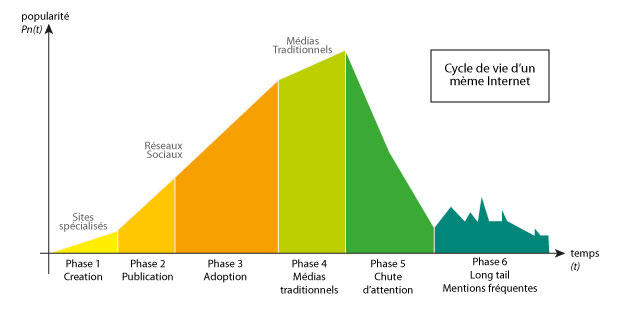
\includegraphics[width=6.2559in,height=3.1559in]{figures/chap2/chapitre2-img2.jpg}
    \caption[Cycle de vie d{\textquoteright}un mème Internet]{Cycle de vie d{\textquoteright}un mème Internet -Clément Renaud - 2013}
    \label{fig:meme-lifecycle}
\end{figure}

L{\textquoteright}évolution du volume de la diffusion permet donc de définir un mème Internet. Néanmoins, il est impossible de donner une estimation du volume minimum pour devenir {\textquotedblleft}mème{\textquotedblright} tant ce chiffre dépend de la population étudiée : il existe des mèmes à très forte diffusion comme le smiley ; d{\textquoteright}autres mèmes se diffusent seulement au sein de groupes d{\textquoteright}individus restreints sans s{\textquoteright}étendre en-dehors. Ainsi, certains mèmes peuvent avoir connu une diffusion très importante dans un groupe, mais rester absolument inconnu du reste de l{\textquoteright}Internet. Une étude de 2012 comparant la diffusion de nombreux mèmes sur Twitter montre que les utilisateurs tendent à choisir les mèmes selon la structure de leur réseau social et le moment d{\textquoteright}exposition, produisant ainsi une grande hétérogénéité des mèmes dans le réseau \citep{Weng2012}. Ainsi, il est hasardeux d{\textquoteright}essayer de décrire le concept de mème par son contenu tant les sujets et les discussions varient. 

Quelques éléments d{\textquoteright}ordre grammaticaux peuvent néanmoins être observés dans la forme que prennent les contenus, appelé parfois {\textquotedblleft}véhicule{\textquotedblright} du mème. Les mèmes qui sont diffusés les plus largement sont composés d{\textquoteright}images et de vidéo. L{\textquoteright}économie d{\textquoteright}attention très limitée de l{\textquoteright}Internet et les modes de lecture sur écran dans un contexte d{\textquoteright}abondance d{\textquoteright}informations font que l{\textquoteright}on privilégie souvent les médias visuels sur le texte \citep{Goldhaber2006}. Un autre élément important est la facilité avec laquelle un message peut être approprié par un utilisateur qui veut le modifier ou tout simplement le diffuser dans le réseau. L{\textquoteright}existence des mèmes est en effet largement conditionnée par la possibilité d{\textquoteright}une diffusion à moindre co\^ut et effort pour l{\textquoteright}utilisateur final, la plupart du temps non-rémunéré. Ici on voit émerger une structure visuelle caractéristique du mème : une image accompagnée d{\textquoteright}une légende écrite en caractères blancs détourés de noir, ou de caractères blancs sur fond noir. L{\textquoteright}utilisation de haut contraste de couleur dans les typographies permet de faire apparaitre très efficacement des légendes juxtaposées à l{\textquoteright}image.

\begin{figure}[h]
    \centering
    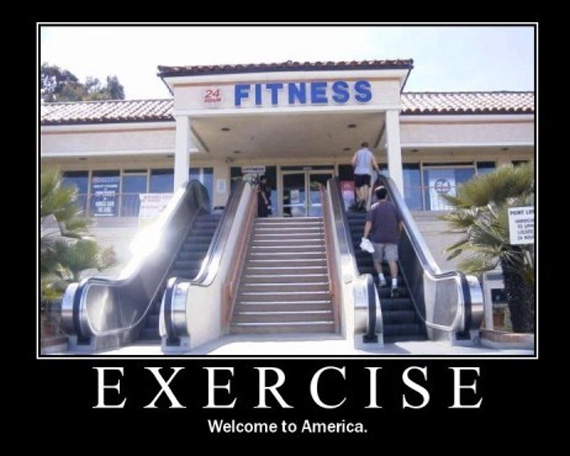
\includegraphics[width=3.6335in,height=2.9114in]{figures/chap2/chapitre2-img3.jpg}
    
\includegraphics[width=2.2559in,height=2.9449in]{figures/chap2/chapitre2-img4.jpg}
    \caption[Exemples de mèmes internet]{Exemples de mèmes Internet, d{\textquoteright}après \url{http://knowyourmeme.org}, consulté le 12/08/2013 à 10 :01 GMT+8}
    \label{fig:memes-examples}
\end{figure}

L{\textquoteright}usage d{\textquoteright}images légendées est une des formes les plus communes pour les mèmes Internet, en particulier ceux de nature comique ou absurde. La mise en place de sites permettant de générer rapidement ce type d{\textquoteright}images légendées (memegenerator.com, mememachine.com, etc.) renforcent l{\textquoteright}unité formelle des mèmes sur l{\textquoteright}Internet, ou plutôt sur l{\textquoteright}Internet anglophone et francophone notamment. En effet, on constate que cette forme typique du mème ne se retrouve pas sur l{\textquoteright}Internet chinois qui utilise plus volontiers des montages d{\textquoteright}images ou des jeux de mots, avec davantage de diversité dans les formes que peuvent prendre les différents mèmes.

\section[Mème, mémoire collective et culture]{Mème, mémoire collective et culture}
\subsection[La mémoire comme trace]{La mémoire comme trace}

Si le concept de mème est souvent considéré comme très récent, on peut néanmoins le resituer dans le vaste paysage des travaux sur la mémoire collective qui ont existé depuis le XIXème siècle \citep{Laurent1999}. Max Stirner dans son livre \textit{The Ego and Its Own }\citeyear{Stirner1995} énonce déjà l{\textquoteright}idée que les individus sont sujets à la circulation de concepts issus de souvenirs communs ou illusoires, comme notamment le nationalisme et la religion. Le logicien Bertrand Russell reprend par la suite dans son livre \textit{The Analysis of Mind } (\citeyear{Russell1921}) les travaux sur la mémoire et l{\textquoteright}évolution sociale du physiologiste allemand \cite{Semon1923}. Utilisant le concept central de \textit{mneme} (du grec 
% μνήμη
\textit{mneme}, mémoire), Semon travaille sur l{\textquoteright}idée de \textit{{\textquotedblleft}traces mnésiques{\textquotedblright} }laissées par les diverses expériences au niveau cellulaire comme au niveau de l{\textquoteright}organisme tout entier. La psychanalyse a également cherché à saisir cette distance impalpable entre expérience et organisme en interrogeant les marques laissées par les souvenirs. Pour Freud comme pour Semon, {\textquotedblleft}l{\textquoteright}appareil psychique{\textquotedblright} de la mémoire se constitue sous la forme de {\textquotedblleft}traces{\textquotedblright}, qu{\textquoteright}il se refuse néanmoins à localiser dans des zones spécifiques du cerveau. Lacan après lui suggèrera que la perception et la mémoire des expériences se structurent dans le langage lui-même, seul outil de connaissance du monde. Depuis les dix dernières années, plusieurs découvertes dans le domaine de la neurologie viennent corroborer cette idée que la mémoire existe sous forme de traces. Les travaux autour de la \textit{plasticité neuronale }montrent notamment l{\textquoteright}existence de la mémoire sous la forme de connections, relations ténues ancrées dans notre réseau neuronal global \citep{Magistretti2008}.  

\begin{table}[htbp]
    \centering
    \begin{tabulary}{\textwidth}{L|C C C}
        
        ~ & t=1  & t=2  & t=3 \\[2ex]
        
        \hline \\ [-1.5ex]
    
        Freud  & expérience  & perception  & Traces mnémiques et psychiques \\[3ex]

        Lacan & expérience (signifié)  &   perception (signifié)  &   Signifiant (traces structurées dans le langage) \\[3ex]

        Neurosciences &  expérience & Perception & Traces synaptiquesassemblages de neurones \\[3ex]

    \end{tabulary}

    \caption{ Etapes constituantes de la mémoire - Convergence entre la trace psychique et synaptique \citep{Ansermet2004} }
\end{table}

Ces disciplines s{\textquoteright}intéressent majoritairement à l{\textquoteright}étude de la constitution d{\textquoteright}une mémoire individuelle, ne nous livrant que peu de clés pour comprendre les éléments qui font qu{\textquoteright}une mémoire devient commune. Le paléontologiste Leroi Gourhan propose dans son livre \textit{L{\textquoteright}homme et la Matière} (\citeyear{Leroi-Gourhan1971}) de considérer que les humains possèdent trois formes de mémoire : une mémoire individuelle sensible, stockée dans les organes du corps ; une mémoire héritée génétiquement, stockée dans l{\textquoteright}ADN ; et une troisième forme de mémoire, transmise de générations en générations : la \textit{technologie}. Dans sa lecture de Leroi-Gourhan, Stiegler (1998b) explique comment \textit{l{\textquoteright}objet technologique} porte en lui les traces des expérimentations, réussites et échecs, mémoire cumulative de temps et de sociétés passées, à la fois héritée et commune, transmissible par son usage.

\begin{table}[htbp]
    \begin{tabulary}{\textwidth}{L|C C}
        \centering
        \textbf{Forme de mémoire} &  \textbf{Contenu}  & \textbf{Stockage} \\[3ex]
        \hline \\ [-1.5ex]
        génétique  &  Particularités héritées des ancêtres   &  DNA \\[3ex]
        
        épigénétique   &  Mémoire sensible de l’expérience personnelle   &  Organes, nerfs, cerveau \\[3ex]
        
        technologique  &  Pratiques de la vie quotidienne en société (usages) & Objets technologiques \\[3ex]
    \end{tabulary}
    \caption{Les trois formes de mémoire d{\textquoteright}après Leroi-Gourhan et Stiegler}
\end{table}


\subsection[Diffusion de mèmes et structuration d{\textquoteright}une mémoire collective]{Diffusion de mèmes et structuration d{\textquoteright}une mémoire collective}
La relation entre mémoire humaine et mémoire technologique est au centre de notre étude. La technologie a depuis toujours été considérée comme une mémoire extérieure. Dans \textit{Phèdre}, Platon raconte l{\textquoteright}histoire du roi égyptien Thamous recevant en cadeau du dieu Thot l{\textquoteright}écriture, le remède (\textit{pharmakon) }qui devait \textit{{\textquotedblleft}soulager la science et la mémoire{\textquotedblright} }(Platon, 274e). Le roi Thamous, effrayé par cette nouvelle technologie de la mémoire écriture se voit saisi de l{\textquoteright}angoisse d{\textquoteright}une perte de cette mémoire. Avec la fin de cette oralité, la disparition de la méthode active des antiques thé\^atres de la mémoire au profit d{\textquoteright}un support inerte et extérieure pourrait-t-elle sceller l{\textquoteright}avènement d{\textquoteright}une nouvelle bêtise? Aujourd{\textquoteright}hui, l{\textquoteright}importance grandissante des bases de données et de connaissances soulèvent encore une fois les mêmes questions, toujours irrésolues. Nicolas Carr constate notamment que \textit{{\textquotedblleft}l{\textquoteright}Internet nous rend stupide{\textquotedblright}} et que son usage répété entraine une baisse drastique de nos facultés de concentration \citep{Carr2010}. A l{\textquoteright}ère du Big Data et de l{\textquoteright}expansion sans fin de notre mémoire numérique, la constitution de nos bases de données interroge notre construction d{\textquoteright}une mémoire collective. Les mèmes Internet, d{\textquoteright}abord gravés dans les disques durs des serveurs, viennent être actualisés par ceux qui les partagent, les commentent, jouent avec et se les approprient. L{\textquoteright}exemple de l{\textquoteright}Internet chinois nous montre la volatilité de cette mémoire numérique, artefact historiographique d{\textquoteright}une culture soumise au bon-vouloir des administrateurs du réseau. Le \textit{Manifeste de l{\textquoteright}Archiviste} publié par \cite{Hui2014} s{\textquoteright}ouvre sur l{\textquoteright}angoissante interrogation deleuzienne :  

\begin{quote}
\textit{
    ``Un nouvel archiviste est nommé dans la ville. Mais est-il à proprement parler nommé ? N'est-ce pas sur ses propres instructions qu'il agit ?''
}
\citep{Deleuze1972a}.
\end{quote}

L{\textquoteright}existence et l{\textquoteright}usage quotidien des bases de données questionnent chaque jour l{\textquoteright}assujettissement des symboles de notre mémoire à l{\textquoteright}objet technologique, à la fois béquille, prothèse et maquillage postiche de notre détestable devenir bête. Les petits \textit{mèmes Internet}, habitant des profondeurs glacées des \textit{data centers}, nous parviennent en dansant, d{\textquoteright}abord sur nos écrans puis dans un coin de notre tête. Avec l{\textquoteright}usage répété des technologies et de l{\textquoteright}écriture numérique, les frontières entre milieu numérique et mémoire collective s{\textquoteright}estompent pour laisser entrevoir un enchevêtrement de silicium, d{\textquoteright}idées et de chair, constitutifs de notre savoir moderne. 

Poursuivant l{\textquoteright}idée d{\textquoteright}une archéologie du présent introduite par Foucault, il s{\textquoteright}agit donc de documenter les processus par lesquels ces obscurs habitants des bases de données viennent laisser leurs traces pour constituer des bribes de nos mémoires collectives. Maurice Halbwachs dans son vaste travail aborde les fa\c{c}ons dont l{\textquoteright}histoire structure l{\textquoteright}être-ensemble des groupes humains. En disant que \textit{"l'histoire de notre vie fait partie de l'histoire en général"}\citep{Halbwachs1947}, il identifie une mémoire autobiographique (personnelle) et une mémoire historique (sociale). Les inquiétudes et considérations autour de la {\textquotedblleft}vie privée{\textquotedblright} sur Internet illustrent les liens intimes entre ces deux mémoires aux frontières devenant aujourd{\textquoteright}hui chaque jour plus poreuses. L{\textquoteright}acte singulier et autobiographique devient sous l{\textquoteright}effet du réseau un fait social, disponible à tout moment dans {\textquotedblleft}l{\textquoteright}historique{\textquotedblright} qui se déroule sous le curseur. L{\textquoteright}oubli devient alors un commerce très prisé permettant de garantir la limite entre la mémoire autobiographique de la fin de soirée de samedi dernier et la mémoire socialement acceptable du CV du chercheur d{\textquoteright}emploi. \'A l{\textquoteright}inverse, les photos du dernier voyage en Papouasie ou la pose avec une star de la télé témoignent fièrement d{\textquoteright}un lien mémoriel entre autobiographie et histoire commune. Les \textit{mèmes} se propagent ainsi d{\textquoteright}individus en groupes pour former peu à peu des éléments de mémoire commune. Objets, chansons, histoires, légendes, icônes... se diffusent autour de la toile par des procédés tenant autant de la copie que de l{\textquoteright}appropriation. 

\begin{figure}[htbp]
    \centering
    
\includegraphics[width=1.6224in,height=1.6224in]{figures/chap2/chapitre2-img5.jpg}
    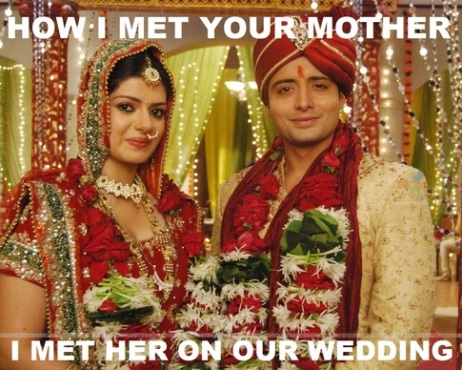
\includegraphics[width=2.0449in,height=1.6335in]{figures/chap2/chapitre2-img6.jpg}
    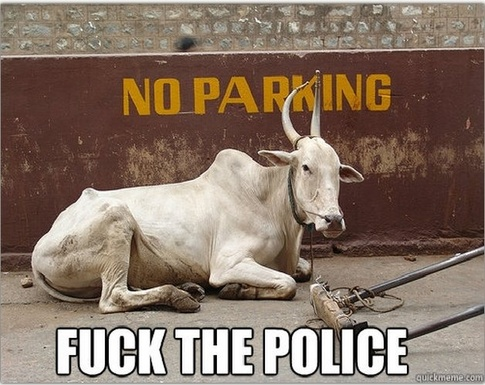
\includegraphics[width=2.078in,height=1.6449in]{figures/chap2/chapitre2-img7.jpg}
    \caption[Réponses à la question à propos des mèmes indiens sur Quora]{Exemples de réponses à la question \textit{"What are some quintessential Indian memes ?"} D'après \url{http://www.quora.com/India/What-are-some-quintessential-Indian-memes}, Consulté le 12/08/2013 à 0 :41 GMT+8 }
    \label{fig:quora-india}
\end{figure}


Le site de questions/réponses \textit{Quora.com} offre un regard intéressant sur la question : \textit{{\guillemotleft}~What are some quintessential Indian memes ?~{\guillemotright}.} Les utilisateurs répondent donc en ajoutant des exemples de mème qui semblent appartenir dans leurs esprits à la {\textquotedblleft}quintessence des mèmes indiens {\textquotedblright}. 
 Avec plusieurs centaines d{\textquoteright}images postées par des
utilisateurs majoritairement indiens, nous pouvons constater plusieurs choses : 

\begin{itemize}
    \item \textbf{Langue}: à part trois réponses, la totalité des réponses sont en anglais. Cela peut s’expliquer par le fait que l’anglais est une langue de communication majoritaire en Inde, et également par le fait que le site Quora.com n’accepte habituellement que des réponses en anglais.
    \item \textbf{Forme}: à l’exception de quatre réponses, les mèmes revêtent tous la forme « classique » : photo retouchée et légendé par un texte en anglais aux lettres blanches sur fond ou détour noir.
    \item \textbf{Humour}: la plupart des réponses sont de nature comique.
    \item \textbf{Récurrence}: certaines images sont très récurrentes et si les légendes diffèrent, le sens reste le même.
    \item \textbf{Thématiques diverses}: de nombreux messages traitent de la vie de famille (parents, mariage), de loisirs (cricket), de la vie quotidienne (achats, école , etc.) et un peu de politique.
\end{itemize}

L{\textquoteright}image la plus citée représente la figure d{\textquoteright}un père autoritaire :

\begin{figure}[htbp]

    \subfloat[\textit{"High Expectations Indian Father"}]{
        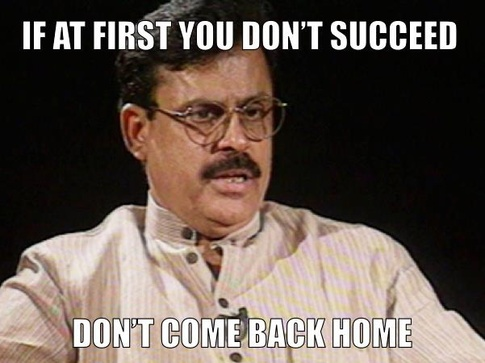
\includegraphics[width=2.0449in,height=1.5in]{figures/chap2/chapitre2-img8.jpg}
        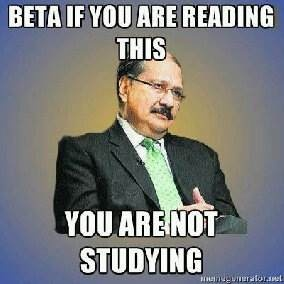
\includegraphics[width=1.5335in,height=1.5in]{figures/chap2/chapitre2-img9.jpg}
        
\includegraphics[width=1.8224in,height=1.5in]{figures/chap2/chapitre2-img10.jpg}
        \label{fig:severe-indian-dad}
    }
    \newline
    \subfloat[\textit{"High Expectations Asian Father"}]{
        \label{fig:severe-chinese-dad}
        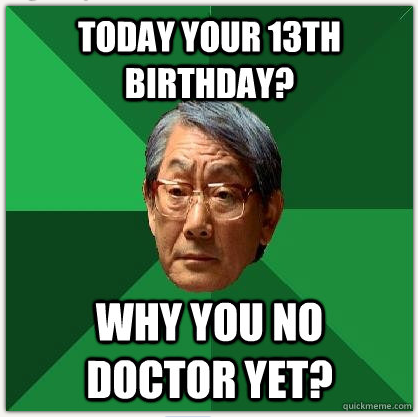
\includegraphics[width=1.9335in,height=1.9in]{figures/chap2/chapitre2-img11.png}
        
\includegraphics[width=1.9004in,height=1.9in]{figures/chap2/chapitre2-img12.jpg}
        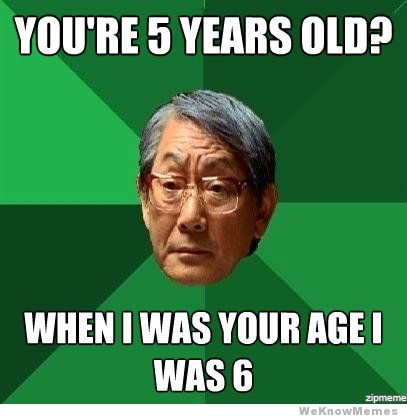
\includegraphics[width=1.8449in,height=1.9in]{figures/chap2/chapitre2-img13.jpg}
    }
    \caption[Mème ``High Expectations Asian Father'' d'après Quora.com]{Exemples du mème \textit{"High Expectations Asian Father"} D{\textquoteright}après {\textquotedblleft}\textit{What are the funniest High Expectations Asian Father meme images?{\textquotedblright}} sur Quora.com \url{http://www.quora.com/Memes/What-are-the-funniest-High-Expectations-Asian-Father-meme-images}, Consulté le 12/08/2013 à 10:56}
\end{figure}

La définition des mèmes faites par Blackmore ne correspond pas nécessairement à ce que nous observons ici. L{\textquoteright}unité formelle de l{\textquoteright}ensemble de ces mèmes (image avec des caractères blancs cerclés de noirs) propose une définition bien plus restreinte. Néanmoins, nous pouvons comprendre qu{\textquoteright}il s{\textquoteright}agit bien de la manifestation d{\textquoteright}une culture particulière. L{\textquoteright}image d{\textquoteright}une vache assise devant un sigle \textit{{\textquotedblleft}Fuck The Police{\textquotedblright} }serait en effet un absolu non-sens sans la référence à l{\textquoteright}Inde o\`u les vaches sont sacrées et jouissent de droits particuliers que même la police ne peut entraver. Ainsi, il existe bel et bien des pré-requis pour comprendre ou actualiser un mème. Les plus évidents sont :

\begin{itemize}
    \item \textbf{L’accès et l’usage de la bonne technologie}: Il est nécessaire pour un utilisateur de posséder et de savoir utiliser la technologie par laquelle le mème est diffusé.
    \item \textbf{La langue}: Le message possède une légende donc l’utilisateur doit pouvoir la lire et la comprendre.
    \item \textbf{Les implicites} : L’utilisateur doit posséder le socle de références communes et d’implicites qui sont impératifs pour pouvoir comprendre le message. 
\end{itemize}

Nous observons ici de très larges et vagues groupes ({\guillemotleft}~\textit{indiens}~{\guillemotright}, {\guillemotleft}~\textit{asiatiques}~{\guillemotright}{\dots}) sans pouvoir vraiment comprendre dans le détail ce qui peut réellement constituer des éléments communs. Les travaux sur la formation des {\textquotedblleft}communautés{\textquotedblright} en ligne ont montré comment la circulation des objets digitaux peut posséder une fonction de catharsis pour des groupes plus réduits \citep{Steyer2006}. Néanmoins, on voit bien qu{\textquoteright}ici l{\textquoteright}appartenance pré-existe puisque le mème nécessite de nombreux pré-requis pour le comprendre. Le langage et son expressivité par l{\textquoteright}humour sont notamment des contraintes incompressibles pour l{\textquoteright}actualisation de ce mème par un individu. Néanmoins nous pouvons voir dans ce cas particulier que le mème participe à l{\textquoteright}affirmation de l{\textquoteright}existence du groupe, avec la figure redondante de caractéristiques communes du père, affirmant par la dérision une forme de paternité commune aux membres de ce groupe. D{\textquoteright}autres mèmes ne nécessitent pas tant de références, ce qui contribue largement à leurs diffusions. La vidéo du clip musical \textit{Gangnam Style} du chanteur Psy a notamment atteint des records inégalés en termes de diffusion\footnote{ Première vidéo à avoir officiellement dépassée le milliard de vues sur Youtube. 1,733,769,243 vues, consulté le 13/08/2013 à 09 :35 GMT+8 \url{http://www.youtube.com/watch?v=9bZkp7q19f0}} gr\^ace à une très vaste campagne télévisuelle et sur internet. La diminution des implicites et la standardisation de l{\textquoteright}écriture utilisée a sans doute contribué la diffusion, avec un langage du corps quasi universel, le pas de danse. Formellement, il s{\textquoteright}agit d{\textquoteright}un vidéo clip très classique dont la structure et le montage sont largement familiers du public. Les attributs des personnages du clip sont également de grands classiques du vidéo clip commercial : voitures, belles filles et bijoux en or. La présence d{\textquoteright}un quartier spécifique de Séoul en Corée du Sud agit ici comme un attribut du contenu mais aucune des références ne nécessite de préalable linguistique particulier. De plus, les mystères de la musique et de la scénographie agissent bien évidemment au-delà de toute analyse formelle pour faire de ce hit un des mèmes Internet les plus connus dans le monde. 
Les méméticiens disposent classiquement de deux procédes pour
analyser la diffusion des mèmes: 

\begin{itemize}
\item
\textbf{La contamination~\newline
}Le mème se déplace à la manière d{\textquoteright}un virus, en contaminant les sujets les plus susceptibles de l{\textquoteright}être lors d{\textquoteright}une phase d{\textquoteright}exposition. L{\textquoteright}exemple le plus classique pour ce modèle est la diffusion des croyances religieuses
qui agirait par contagion \citep{Dennett2006}
\item
\textbf{La réplication~\newline
L}es activités culturelles humaines procèdent de l{\textquoteright}imitation, notamment au travers de phases cruciales d{\textquoteright}apprentissage. Ainsi, les mèmes existent et se diffusent dans toutes activités nécessitant une imitation : \textit{{\textquotedblleft}} \textit{If we define memes as transmitted by imitation then whatever is passed on by this copying process is a meme.{\textquotedblright} }\citep{Blackmore2006}. 
\end{itemize}

Le modèle épidémique de diffusion vient appuyer la vision éthologique du mème. Adaptée de la virologie, les {\guillemotleft}~sujets à risque~{\guillemotright} seraient plus à même d{\textquoteright}être {\guillemotleft}~contaminés~{\guillemotright} par une {\guillemotleft}~exposition~{\guillemotright} suffisamment longue à tel ou tel mème \citep{Wang2011}. Blackmore définit néanmoins trois phases indispensables pour reconna\^itre un mème comme tel:  

\begin{quote}
\textit{``Memes fulfill the role of replicator because they exhibit all three of the necessary conditions; that is, \textit{heredity} (the form and details of the behavior are copied), \textit{variation} (they are copied with errors, embellishments or other variations), and \textit{selection} (only some behaviors are successfully copied).''}, d'après \cite{Blackmore2006}
\end{quote}

Les trois aspects sont indissociables et forment selon Blackmore un {\textquotedblleft}\textit{véritable processus évolutioniste{\textquotedblright} }\citep{Blackmore2006}. La définition quasi tautologique du mème ({\guillemotleft}~\textit{Whatever is passed on{\guillemotright}}) montre bien comment le mème en tant que concept est considéré chez Blackmore non pas comme un phénomène mais plutôt comme un objet en-soi. La définition du mème en tant qu{\textquoteright}objet autonome se heurte dès l{\textquoteright}abord au risque de devenir un pur artefact de l{\textquoteright}observation, n{\textquoteright}existant que dans l{\textquoteright}esprit de l{\textquoteright}observant. Alors que Dawkins met en garde non sans humour que son livre \textit{The Selfish Gene} \textit{{\textquotedblleft}devrait être lu presque comme s{\textquoteright}il était de la science-fiction{\textquotedblright} }\citep{Dawkins1989}, la faiblesse des modèles de diffusion des mèmes vu comme un réplicateur ou comme un virus ne recouvre que partiellement la réalité observée empiriquement pour les mèmes Internet. Ainsi, l{\textquoteright}appartenance des individus à tel ou tel groupe pré-existe au mème. Dans son appropriation se joue davantage l{\textquoteright}expression d{\textquoteright}un sentiment d{\textquoteright}appartenance qu{\textquoteright}une contamination qui nierait les termes de sa volonté individuelle pour y substituer l{\textquoteright}individu comme sujet du mème.  


\section[Textualité des mèmes et formes d{\textquoteright}énonciations numériques]{Textualité des mèmes et formes d{\textquoteright}énonciations numériques}

\subsection[Le mème comme figure rhétorique de l{\textquoteright}écriture intertextuelle]{Le mème comme figure rhétorique de l{\textquoteright}écriture intertextuelle}

 
Le mème peut être défini comme une série d{\textquoteright}actes \textit{d{\textquoteright}énonciation} qui contribuent à l{\textquoteright}existence et la reconnaissance mutuelles d{\textquoteright}individus comme groupe. Cette définition s{\textquoteright}oppose à l'idée d{\textquoteright}une entité de sémantique autonome qui serait constitutif d{\textquoteright}une hypothétique culture commune. Les partages, commentaires, réappropriations puis transformations des \textit{mèmes Internet }nous serviront de supports pour comprendre les \textit{actes d{\textquoteright}énonciation. }Ces courts messages faits de texte, image ou vidéo sont en quelque sorte les voix, répétitions, annonances et redites d{\textquoteright}une foule d{\textquoteright}individus et de groupes qui habitent la Toile. Au-delà de l{\textquoteright}idée d{\textquoteright}un {\textquotedblleft}objet{\textquotedblright} numérique qui réifierait les actions en une substance figée, nous nommons \textit{énonciation} le moment d{\textquoteright}existence observable o\`u se manifeste un mème. Comme pour les émoticones, les pratiques actuelles de l{\textquoteright}écriture en ligne des mèmes Internet sont à envisager comme des formes renouvelées d{\textquoteright}oralité. Email, chat ou réseaux sociaux, ces discussions font partie d{\textquoteright}une \textit{{\textquotedblleft}oralité seconde{\textquotedblright} }\citep{Ong1988} constituante des technologies de l{\textquoteright}écrit à l{\textquoteright}ère du numérique. Contrairement à l{\textquoteright}oralité première des illettrés, cette oralité seconde est structurée par l{\textquoteright}usage des technologies et notamment les structures formelles de l{\textquoteright}écriture pour le média :  

\begin{quote}
    \textit{``Telephone, radio, television and the various kind of sound tape, electronic technology has brought us into the age of {\textquoteleft}secondary orality{\textquoteright}. This new orality has striking resemblance to the old in its participatory mystique, its fostering of a communal sense, its concentration on the present moment, and even its use of formulas. But it is essentially a more deliberate and self-conscious orality, based permanently on the use of writing and print, which are essential for the manufacture and operation of the equipment and for it use as well.''} 
\citep{Ong1988}
\end{quote}

L{\textquoteright}hypothèse de Ong est ici que l{\textquoteright}oralité des écritures numériques est une forme manufacturée de l{\textquoteright}expression orale, à laquelle préside la production (industrielle) des technologies. Les services de réseaux sociaux en ligne confirment l{\textquoteright}hypothèse première de Ong puisque \textit{Sina Weibo }ou \textit{Twitter} contraint industriellement l{\textquoteright}écriture à une longueur maximum de 140 caractères. Néanmoins, l{\textquoteright}oralité du mème Internet et plus généralement des écritures numériques ne procède pas seulement de cette écriture conditionnée mais également de la mise en relation des textes : l{\textquoteright}intertextualité. Là o\`u pour Ong l{\textquoteright}industrie médiatique vient contraindre l{\textquoteright}écriture pour la réifier en produit industriel simulant l{\textquoteright}oral, l{\textquoteright}intertextualité vient subvertir ces limites imposées en renvoyant le lecteur à la page suivante.  

En effet, le langage des nouveaux médias ne se contente pas de proposer des nouvelles opérations d{\textquoteright}interactions et de navigations mais s{\textquoteright}inscrit également dans de nouveaux modes de lecture et de narration \citep{Manovich2001}. Une des grandes difficultés pour l{\textquoteright}analyse textuelle et narrative dans le cadre des nouveaux médias est de comprendre o\`u commence et o\`u se termine le texte. La structure éminemment relationnelle du discours narratif en ligne et son intertextualité en font un objet mal défini, que ses auteurs n{\textquoteright}ont pas signé d{\textquoteright}un point final. L{\textquoteright}étude des discursivités hypertextuelles s{\textquoteright}apparenterait donc davantage à l{\textquoteright}étude des formes dans les contes et légendes qu{\textquoteright}aux études herméneutiques classiques sur des textes finis \citep{Clement1995}. Comme le note Lévi-Strauss dans son travail sur Propp, même si les contes possèdent souvent une structure similaire, leur étude en tant qu{\textquoteright}élément culturel n{\textquoteright}est révélatrice que dans un contexte précis et incarné. Il est inutile de vouloir extraire une supposée intention culturelle du texte car on se doit de le comprendre lors de son énonciation, sur la place d{\textquoteright}un marché au Maroc avec les conteurs de Ben Jelloun ou au pied du lit d{\textquoteright}un jeune Européen avec les histoires compilées par les frères Grimm. Héritant à la fois des pratiques culturelles et folkloriques anciennes tout en se renouvelant sous les nouvelles contraintes de la technologie \citep{Barber2008}, le mème est lui aussi à comprendre dans son contexte d{\textquoteright}énonciation. De récents travaux travaillent à comparer les modes de diffusion des mèmes avec ceux des traditions folkloriques \citep{Seta2014}. En considérant les mèmes Internet comme un {\textquotedblleft}\textit{folklore numérique}{\textquotedblright}, on comprend mieux la nature presque auto-référentielle de la relation entre le mème et la culture qui le voit na\^itre. La transmission d{\textquoteright}éléments particuliers dans la discursivité du mème en fait une figure rhétorique d{\textquoteright}énonciation de sa propre origine. 

Le large pouvoir fédérateur de certains mèmes fascine. Diffusés très largement, \ on se plait à imaginer comment ils peuvent réunir en leur sein des groupes et individus distants, auparavant inconnus et étrangers. L{\textquoteright}importance croissante d{\textquoteright}Internet dans l{\textquoteright}émergence de groupes d{\textquoteright}intérêts et d{\textquoteright}activités voit les études sur la formation de communautés en ligne fleurir. Néanmoins, il nous semble important de se questionner sur la nature des relations créée lors des discussions partagées en ligne. Est-ce bien là le fait d{\textquoteright}une réelle rencontre comme le croient les plus enthousiastes? Ou au contraire est-ce le produit d{\textquoteright}une machine médiatique et décérébrante qui produit du lien sans engendrer de rencontres comme le pensent les plus pessimistes? Cette vaste question est sans doute un des enjeux centraux des questionnements autour de l{\textquoteright}Internet, notamment pour le management et les sciences de gestion. Si l{\textquoteright}énonciation est une pratique structurante pour un individu ({\textquotedblleft}je suis{\textquotedblright}), elle peut l{\textquoteright}être également pour un groupe ({\textquotedblleft}nous sommes{\textquotedblright}). Dans la perspective empirique o\`u nous nous situons, il nous faut tout d{\textquoteright}abord interroger les pratiques du langage pour mieux comprendre comment les discursivités d{\textquoteright}un mème peuvent agir sur les groupes. Le mème considéré comme un acte d{\textquoteright}énonciation se caractérise non seulement par sa manifestation langagière, mais également par l{\textquoteright}intention qu{\textquoteright}il contient. Dans le cadre des réseaux sociaux, nous ne disposons que de très peu d{\textquoteright}éléments sur l{\textquoteright}intention car les données disponibles sur les réseaux sociaux sont par définition le résultat d{\textquoteright}actions passés (écriture, clics, etc.).\textit{ }Nous devons donc développer un modèle à la fois conceptuel et pratique pour nous permettre d{\textquoteright}étudier ces phénomènes d{\textquoteright}énonciation dans le cas particulier des mèmes Internet. Wittgenstein dans ses \textit{Recherches Philosophiques }défend une analyse pragmatique du langage en écrivant : \textit{{\textquotedblleft}Don{\textquoteright}t ask for the meaning, ask for the use.{\textquotedblright}} \citep{Wittgenstein2004}. Il s{\textquoteright}agit de comprendre les jeux langagiers non pas comme un champ linguistique mais comme un ensemble d{\textquoteright}actes qui font sens en contexte et possèdent une intention. 

\begin{quote}
{\textquotedblleft}
\textit{Expressions have meanings even when they are not being used, but it is only in using expressions that a person means something.}
{\textquotedblright} \citep{Bach1994}
\end{quote}

Austin dans ses lectures sur William James met au centre du langage sa dimension pragmatique et propose de comprendre comment on \textit{{\guillemotleft}~fait des choses avec les mots~{\guillemotright}} \citep{Austin1975}. Ses le\c{c}ons présentent une manière nouvelle de catégoriser les différents actes d{\textquoteright}énonciation et montrent la grande diversité des éléments non-linguistique présents dans ces actes. Austin introduit le concept de \textit{performativité }pour nommer le processus qui permet de construire par le langage une réalité extérieure au langage. Les mots ne nomment pas seulement les choses mais peuvent également les faire changer, voire les fabriquer. Austin s{\textquoteright}intéresse donc aux énoncés selon leurs \textit{sens}, leurs intentions (la \textit{force}) ou leurs \textit{effets}. Le concept de \textit{performativité }a depuis continué son chemin tant en linguistique qu{\textquoteright}en sciences sociales, et plus récemment dans des champs aussi divers que le management ou l{\textquoteright}étude du discours scientifique et des pratiques légales \citep{Denis2006}. Les économistes également ont beaucoup discuté de la performativité des discours économiques sur l{\textquoteright}économie réelle \citep{Mackenzie2006}. Les \textit{cultural studies,} et plus précisément les \textit{gender studies }ont aussi fait un large usage de ce concept pour exprimer l{\textquoteright}influence de la matérialité des mots sur les comportements humains \citep{Butler1993}.  

\begin{quote}
    {\guillemotleft}~\textit{Pour qu{\textquoteright}ils deviennent de {\guillemotleft} véritables {\guillemotright} performatifs, les faits, les théories ou les formules doivent circuler dans des cha\^ines de traduction qui consolident l{\textquoteright}assemblage des entités qui le composent et leur permet d{\textquoteright}acquérir le statut de {\guillemotleft} matters of fact {\guillemotright} ({\dots}). C{\textquoteright}est lorsqu{\textquoteright}ils arrivent à durer, c{\textquoteright}est-à-dire à s{\textquoteright}inscrire dans le monde (par l{\textquoteright}intermédiaire d{\textquoteright}objets, de textes, de dispositifs techniques complexes) que leur performativité s{\textquoteright}accomplit.}~{\guillemotright} \citep{Denis2006}
\end{quote}

Les actes d{\textquoteright}énonciation répétés modèlent donc le corps des personnes et de la société, y \textit{laissant }durablement leurs marques. Les énoncés actualisent les discours des groupes sociaux sur eux-mêmes \citep{Butler1993} et ce caractère performatif est constitutif de l{\textquoteright}énonciation. Les énoncés collectifs que sont les mèmes Internet possèdent également cette dimension performative qui actualise le discours de certains groupes en réalités tangibles. La circulation et la structuration de ces mèmes vient structurer le milieu numérique et peut ainsi influer sur la définition de groupes sociaux et des rapports qu{\textquoteright}ils entretiennent. \'Enoncer à son tour une image ou un mot semble un préalable permettant de dénouer l{\textquoteright}implicite de l{\textquoteright}énoncé et d'accroître la proximité dans l{\textquoteright}expérience. Blackmore évoque en termes évolutionnistes le {\textquotedblleft}potentiel transformatif{\textquotedblright} du mème, avec ce qu{\textquoteright}elle nomme la \textit{variation} puis la \textit{sélection}. Ici ce sont les actes d{\textquoteright}\textit{énonciation} qui forment une praxis du mème. Pour nous, le mème n{\textquoteright}est pas un méta-symbole en évolution mais un réseau de praxis culturelles constitué de multiples d{\textquoteright}actes d{\textquoteright}énonciation. Ainsi, le mème ne peut être simplement {\guillemotleft}~copiée~{\guillemotright} mais a besoin d{\textquoteright}être acté pour exister. Dans la définition du mème de Blackmore comme dans le cas des réseaux sociaux, nous observons que l{\textquoteright}énonciation d{\textquoteright}un mème procède d{\textquoteright}une variation parfois nulle, parfois minimale, parfois importante de sa forme d{\textquoteright}origine. Cette déformation due à l{\textquoteright}énonciation est le propre de la fonction d{\textquoteright}apprentissage, notamment langagier. Le caractère performatif du mème devient visible dans l{\textquoteright}usage approprié de la variation qui en est fait. 

Le succès de l{\textquoteright}intention de l{\textquoteright}énoncé est visible dans son imitation, avec comme garantie l{\textquoteright}erreur ou la variation. Platon dans \textit{La République} puis par la suite Aristote dans sa \textit{Poétique,} s{\textquoteright}interroge sur la notion de \textit{mimesis} définie comme les formes d{\textquoteright}imitation qui permettent soit de reproduire, soit de styliser la nature. Pour Aristote, le but singulier de la mimesis est de mettre à jour la dimension empathique cachée de la nature, de la styliser pour y révéler le continuum de l{\textquoteright}expérience propre à tous les êtres. Plus l{\textquoteright}artiste s{\textquoteright}approche de la nature en se dirigeant vers une imitation {\guillemotleft}~véritable{\guillemotright}, plus il s{\textquoteright}éloigne de la réalité de la nature. L{\textquoteright}importance d{\textquoteright}une approche rhétorique comme par exemple la stylisation devient le véritable moyen d{\textquoteright}accès à la signification profonde des choses. Freud réutilisera le concept de \textit{mimesis} pour décrire l{\textquoteright}énonciation du sens d{\textquoteright}un évènement traumatique passé dans la vie d{\textquoteright}un individu au travers d{\textquoteright}activités créatives (art, parole, rêves etc.). Dans la continuité d{\textquoteright}Aristote, Freud comprend le rêve comme une \textit{mimesis} du passé et du réel, révélant au sujet un objet symbolique enfoui. Peut-être est-il possible de considérer le mème Internet comme une mimesis des groupes sociaux et médiatiques qui le produisent. Les processus de symbolisation et de stylisation jouent en effet un rôle déterminant dans sa diffusion. Acte d{\textquoteright}énonciation, le mème agit alors comme une \textit{mimesis} des activités et états d{\textquoteright}\^ame de groupes d{\textquoteright}individus qui l{\textquoteright}énoncent. S{\textquoteright}il est possible de le revivre plusieurs fois, il prendra peut-être à chaque fois un sens différents. Comme le rêve freudien qui est une manifestation biologique de la mémoire inconsciente se produisant durant le sommeil, le mème se manifeste sous des formes visibles symboliques incarnées, \textit{mimesis} particulière du groupe des individus qui l{\textquoteright}énoncent. 


\subsection[Typologie des mèmes Internet]{Typologie des mèmes Internet}

Habituellement définie comme \textit{{\guillemotleft}~une forme typique de relation non linguistique entre des éléments discursifs.~{\guillemotright}}\footnote{ \textit{Les figures de rhétorique}, Laurent Jenny, Université de Genève, 2003}\textit{, }la figure rhétorique se produit dans l{\textquoteright}intertextualité des redites et commentaires qui réaffirme dans le mème l{\textquoteright}existence d{\textquoteright}un groupe qui le constitue.  

En nous appuyant sur la littérature concernant les figures
rhétoriques, nous pourrions chercher à définir plus
précisément une typologie des mèmes fondée sur les formes du
discours. En grec ancien, le topo\"i défini à la fois un lieu ou un
endroit mais également un ensemble de formes rhétoriques utilisant
des motifs particuliers lors de l{\textquoteright}argumentaire afin de
persuader lors de joutes oratoires. En littérature comme en
mathématiques, le terme de \textit{topos }définit également un
ensemble de catégories ouvertes mais connues,
\textit{{\textquotedblleft}un protocole de description des univers
possibles{\textquotedblright} }\citep{Badiou2006}. Le mème peut donc
être compris comme un \textit{lieu commun, }idée
{\textquotedblleft}re\c{c}ue{\textquotedblright} utilisant des
situations ou des images communes et stéréotypées pour opèrer
une transformation sémantique en jouant sur la répétition
d'éléments (les sèmes du discours). En
rhétorique, l{\textquoteright}usage du topos a pour objectif de
contribuer à la persuasion de l{\textquoteright}auditeur par la
mobilisation subtile d{\textquoteright}éléments de culture commune.
Tout l{\textquoteright}art du rhéteur consiste à trouver un moyen
subtile d{\textquoteright}actualiser un lieu commun en une situation
unique propre au contexte pour convaincre. Dans le discours, il prend
bien souvent la forme de l{\textquoteright}anecdote que la rumeur se
charge de diffuser, sa diffusion étant d{\textquoteright}autant plus
efficace qu{\textquoteright}il possède un caractère amusant ou
railleur \citep{Flaubert1997} Concevoir le mème comme une forme de
pratique rhétorique semblable au lieu commun nous permet de resituer
le phénomène des mèmes Internet dans la continuité historique
des pratiques de l{\textquoteright}écriture et de
l{\textquoteright}énonciation rhétorique, ainsi que de ses
modèles d{\textquoteright}analyse socio-textuelle et littéraire
\citep{Plantin1993}. Ainsi, nous pouvons aborder la lecture des mèmes
Internet sous le jour de leur existence aussi bien formelle (textuelle)
que rhétorique (comme actes d{\textquoteright}énonciations et de
persuasion). Les mèmes tout comme les lieux communs se donnent à
voir d{\textquoteright}abord sous la forme de paradoxes, qui
deviendront eux-mêmes des lieux communs.
L{\textquoteright}originalité d{\textquoteright}un lieu commun en
devenir se définit dans une tension constante entre imitation et
nouveauté, subversion et actualisation de formes canoniques :
\textit{{\textquotedblleft}dialogue de l'horizon
d'attente et de l'écart esthétique, c'est-à-dire le jeu du classique et du moderne, la tension entre le même et l'autre qui existe, dans tout texte et dans toute lecture, entre le plaisir et la jouissance, pour reprendre les mots de Barthes}. \citep{Compagnon1997}

L{\textquoteright}approche des mèmes renouvelée par la nature intertextuelle du langage multimédia montre des caractéristiques  d{\textquoteright}après une centaine de mèmes parmi les plus largement diffusés d{\textquoteright}Internet \citep{Bauckhage2011} :

\begin{enumerate}
\item {\color{black}
\textbf{Humour~}: Le mème doit posséder une dimension comique et
accrocheuse}
\item {\color{black}
\textbf{Intertextualité} : Le mème met en jeu un ou des renvois à
d{\textquoteright}autres éléments culturels ou textuels, souvent
implicites.}
\item {\color{black}
\textbf{Juxtaposition atypique} : Les éléments visuels ou
sémantiques mis en jeu dans le mème ne possèdent pas de
corrélations apparentes et c{\textquoteright}est la mise en relation
de plusieurs objets improbables qui en fait un objet intéressant.}
\end{enumerate}
L{\textquoteright}étude en question nous offre un début de
critères mais porte seulement sur un type précis de mèmes à
caractère plutôt comique, ignorant les discussions plus
sérieuses, d{\textquoteright}ordre politique notamment. La forme
particulière de juxtaposition atypique observée par les auteurs
serait en rhétorique une {\textquotedblleft}\textit{métaphore in
praesentia{\textquotedblright} }décrite comme une
\textit{{\guillemotleft}~figure de rapprochement analogique entre deux
représentations co-présentes~{\guillemotright}} \citep{Jenny2012}. Nous
nous trouvons donc en présence d{\textquoteright}une forme
particulière de mème seulement. Si l{\textquoteright}humour sous
toutes ces formes (blague, sarcasme, ironie, etc.) est un élément
très répandu qui favorise la circulation des contenus en ligne, il
nous semble néanmoins un peu réducteur de se limiter à cette
définition. De nombreux mèmes Internet existent non pas gr\^ace à
l{\textquoteright}humour mais gr\^ace au \textit{pathos}
qu{\textquoteright}ils dégagent. Le mème \textit{Kony2012, }un des
plus diffusés de l{\textquoteright}histoire
d{\textquoteright}Internet, présentait le militaire Ugandais Joseph
Kony dans une vidéo faite d{\textquoteright}images de guerre et
d{\textquoteright}enfants en pleurs\footnote{ \textit{KONY2012: See How Invisible Networks Helped a Campaign Capture the World's Attention}, \textit{Social Flow}, \url{http://alturl.com/zniry} consulté le 28 Février 2014 GMT+1}.
Ainsi, on peut dire que les mèmes Internet utilisent les formes
classiques de la rhétorique adaptées au langage médiatique moderne, 
teinté d{\textquoteright}humour ou de sensationnalisme. En se
saisissant du monde social et politique, les mèmes Internet
produisent d{\textquoteright}intéressants discours sur les faits
qu{\textquoteright}ils relatent - et sur la technologie qui les
produit. Alors que les révolutions du Printemps Arabe avaient
notamment soulevé l{\textquoteright}espoir d{\textquoteright}un monde
meilleur par l{\textquoteright}usage des réseaux sociaux pour
instaurer la démocratie \citep{Lotan2011}, la communication
instantanée via ces mêmes réseaux sociaux devenait quelques
semaines plus tard une des causes majeures de la flambée de violence
durant une série d{\textquoteright}émeutes à Londres \citep{Casilli2011}. Les différentes intentions des discursivités et
actes d{\textquoteright}énonciation à l{\textquoteright}{\oe}uvre
dans un mème peuvent donc nous aider à dresser une typologie des
mèmes. Une typologie des mèmes ne peut être considérée comme
exclusive et les glissements sémantiques et symboliques qui peuvent
s{\textquoteright}opérer nous obligent à considérer une
catégorisation non-exclusive. En nous appuyant sur différents
exemples et sur la littérature, nous dressons une première
ébauche de typologie des mèmes Internet qui sera ensuite
approfondie par l{\textquoteright}étude empirique des données le
c{\oe}ur de notre étude. Pour les exemples, nous essaierons de donner
les références et implicites indispensables permettant de
comprendre le mème dans son intertextualité.

\begin{table}[htbp]
    \centering
    \begin{tabulary}{\textwidth}{ R | C}
    \textbf{Objectifs du mème}  & \textbf{Exemples célèbres et références} \\[1ex]
    \hline \\ [-1.5ex]
    Absurdiste, humour &  LOLCats, Tumblr \citep{Bauckhage2011} \\[1ex]
    \hline \\ [-1.5ex]
    Actualité, satire, commentaire social  & CaoNiMa \citep{Mina2012}, Cute Cat Theory \citep{Zuckerman2008} \\[1ex]
    \hline \\ [-1.5ex]
    Publicité, marketing viral & Gangnam Style \citep{Bolsover2013}, Memetic Marketing \citep{Flor2000} \\[1ex]
    \hline \\ [-1.5ex]
    Marketing politique, soutien, pétition & Obama Ohio Campaign \citep{Walker2012}, Pétitions en ligne (Adamic al.,2013) \\[1ex]
    \hline \\ [-1.5ex]
    Fan clubs, adoration  &  Fan-fiction , Machinima, etc. \\[1ex]
    \hline \\ [-1.5ex]
    Hoax, spam & Email spam, « Nigerian scam » \\[1ex]
    \end{tabulary}

\caption[Typologie des mèmes]{Les différents type de mèmes Internet observables - tableau réalisé d{\textquoteright}après la littérature indiquée}
\label{fig:typologie-memes}

\end{table}


Cette typologie nous permet de poser un premier regard sur des catégories non-exclusives constituant le paysage des mèmes Internet, inspirés d{\textquoteright}exemples et de la littérature existante. Nous pouvons d{\textquoteright}ores et déjà noter que l{\textquoteright}ensemble de ces différentes pratiques pré-existent à l{\textquoteright}Internet et sont souvent la reconduction sous une forme numérique de discursivités pré-existantes (penser à la publicité, la propagande politique ou même les rumeurs). La forme et l{\textquoteright}échelle de la diffusion sont néanmoins des différences importantes ainsi bien s\^ur que \ les situations d{\textquoteright}énonciation (dans une file d{\textquoteright}attente ou devant son ordinateur).

\begin{description}

\item[Absurdiste, humour]
\hfill \\
De nombreux mèmes Internet parmi ceux que nous avons présentés dans la première partie de ce chapitre viennent se classer dans cette catégorie. Connaissant parfois des succès planétaire, un des exemples les plus caractéristiques est celui des {\textquotedblleft}LOLcats{\textquotedblright}, ces vidéos ou images de chats illustrés de citations et autres accessoires comiques. Omniprésent sur la Toile, l{\textquoteright}immense répertoire de photos et de vidéos comiques de chats dans différentes situations (jouant du piano, sautant dans des bo\^ites en cartons, etc.) constitue un des plus visionnés de l{\textquoteright}Internet \citep{Bauckhage2011}.

\begin{figure}[htpb]
    \centering
    
    \subfloat[a LOLcat]{
        
\includegraphics[scale=.72]{figures/lolcats/cat7.jpg}
    }
    \subfloat[another LOLcat]{ 
        
\includegraphics[scale=.15]{figures/lolcats/lolcat_00294386.jpg}
    }
    \caption[Some LOLcats]{Some LOLcats, d{\textquoteright}après le \url{http://www.lolcats.com}, consulté le 4 Avril 2013 à 15:32}
    \label{fig:caonima}
\end{figure}



\item[Actualité, satire, commentaire social]
\hfill \\
En regroupant ces trois catégories, nous souhaitons considérer la pratique ancienne des discussions politiques ou polémiques autour de faits divers ou d{\textquoteright}actualités que l{\textquoteright}Internet vient aujourd{\textquoteright}hui renouveler dans la forme. Nous avons vu précédemment avec les {\textquotedblleft}crabes de rivières{\textquotedblright} (voir \ref{fig:hexie}) comment la satire politique en Chine se manifestait bien souvent sous la forme de mèmes Internet. Par les voies de l{\textquoteright}Internet,de nombreux faits divers sont devenus en Chine des affaires d{\textquoteright}état, influen\c{c}ant le jeu politique et offrant un nouveau canal de diffusion pour les pratique subversives. Connu pour son {\oe}uvre artistique, l{\textquoteright}artiste chinois Ai Weiwei est une des figures célèbres de l{\textquoteright}Internet chinois. Utilisant abondamment blog et microblog, son travail artistique depuis plusieurs années a pris la tournure d{\textquoteright}un bras de fer médiatique avec le gouvernement sur les grandes questions sociétales de la Chine d{\textquoteright}aujourd{\textquoteright}hui. Son père, poète célèbre du régime communiste sous Mao fut déchu durant la révolution Culturelle, transmettant à son fils à la fois un go\^ut pour les arts et une violente amertume pour le pouvoir en place à Pékin. Critiquant ouvertement la corruption des officiels et de la police, Ai Weiwei a vu régulièrement ses comptes Internet de blog et microblog fermés, notamment par le service Sina Weibo. Sur Twitter néanmoins, il jouit d{\textquoteright}une grande popularité avec près de de 200.000 \textit{{\textquotedblleft}followers{\textquotedblright}} pour son compte officiel @aiww. Au fil de son blog relatant ses nombreux déboires avec le gouvernement, on croise bien souvent une figure mythologique né de la toile chinoise, le \textit{caonima}.  

\begin{figure}[htpb]
    \centering
    
    \subfloat[Une image de la vidéo originale représentant le \textit{caonima}.]{
        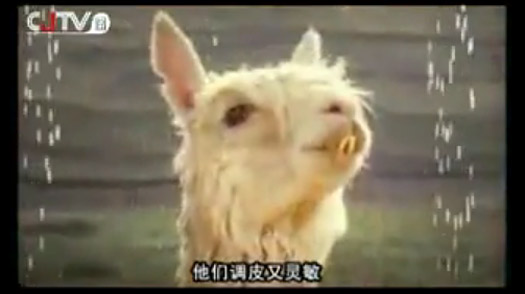
\includegraphics[width=3.7894in,height=2.1224in]{figures/chap2/chapitre2-img14.jpg}
    }
    \subfloat[Un caractère chinois composé spécialement par les internautes pour signifier cet animal mythique]{ 
        
\includegraphics[width=2.0559in,height=2.0559in]{figures/chap2/chapitre2-img15.jpg}
    }
    \caption[\textit{Caonima}: un animal mythique du web chinois]{\textit{Caonima}: un animal mythique du web chinois, d{\textquoteright}après le \textit{Grass-Mud Horse Lexicon Classics}publié par \textit{China Digital Times }(2013)}
    \label{fig:caonima}

\end{figure}

Luttant contres les crabes de rivière, le \textit{caonima }symbolise la lutte contre la censure pour un Internet libre. Apparu pour la première fois dans une vidéo virale\footnote{ \textit{Song of the Grass-Mud Horse (Cao Ni Ma), }Youtube \ \url{https://www.youtube.com/watch?v=wKx1aenJK08}, consulté le 28 Février 22:08\par }, le \textit{caonima} est un animal de la famille des camélidés (l{\textquoteright}alpaga) courant fièrement dans les prés sur une petite musique de dessin animé aux paroles entièrement réécrites pour l{\textquoteright}occasion. Littéralement {\textquotedblleft}cheval d{\textquoteright}herbe et de boue{\textquotedblright}, le mot {\textquotedblleft}caonima{\textquotedblright} (\zh{草泥马})cache en fait un double sens puisque son homophone (\zh{操你妈}) est une grossière interjection à l{\textquoteright}intention des génitrices des censeurs de Pékin. Devenu aujourd{\textquoteright}hui une véritable icône anti-censure, il n{\textquoteright}est pas rare de le croiser sur un tee-shirt ou accroché à un sac dans de nombreux endroits improbables en Chine. Comme le note très justement An Xiao Mina : \textit{{\textquotedblleft}les mèmes sont les graffitis du web censuré{\textquotedblright}} \citep{Mina2012}. Malgré le zèle des pouvoirs publics à les effacer le plus rapidement possible, ils témoignent de l{\textquoteright}existence de réalités occultées qui se manifestent souvent de manière dérisoire, grotesque et improbable, mais sont énoncées malgré tout. 

\item[Publicité et marketing viral]
\hfill \\
La popularité des services de réseaux sociaux a entra\^iné de nombreuses marques à se concentrer sur ce nouveau média pour mener leurs campagnes de publicité et de promotion. Les utilisateurs chinois sont très fortement engagés dans la création de nouveaux contenus avec 76\% des
utilisateurs chinois créant davantage de contenus qu{\textquoteright}ils n{\textquoteright}en lisent, contre seulement 20\% en France \citep{Forrester2013}. Ainsi, de nombreuses marques cherchent à concevoir des interactions en ligne utilisant les mèmes comme véhicule de messages commerciaux afin de
mettre à contribution les internautes dans la diffusion de leur marque. Une des stratégies marketing les plus répandues consiste à créer un \textit{hashtag} amusant afin d{\textquoteright}inciter les internautes à s{\textquoteright}en saisir, le partager et créer de nouveaux
contenus. La marque de préservatifs \textit{Durex} a notamment connu un large
succès avec le hashtag \textit{\#BienEtreNocturne} (en Chinois \#\zh{夜福利}) sur Sina Weibo. Drôle et un peu osé, cette campagne a généré un fort engagement des internautes, contribuant largement à la propagation du profil utilisateur et du nom de la marque \citep{Shi2012}. En récupérant les données des utilisateurs impliqués dans la diffusion, la marque peut également procéder à un travail statistique d{\textquoteright}analyse pour mieux conna\^itre les utilisateurs intéressés par ses produits.Ce type d{\textquoteright}information s{\textquoteright}avère précieuse dans un marché chinois en mouvement o\`u il existe un fort besoin pour des études de marché précises auprès de segments de populations actifs en ligne (adolescents, jeunes, classe moyenne émergente...) \citep{Bergstrom2012}. Malgré le paysage morcelé des services de réseaux sociaux chinois, les utilisateurs chinois semblent davantage enclins à suivre et interagir avec les marques que leurs homologues américains notamment\footnote{ D{\textquoteright}après Ken Hong, Sina Weibo General Marketing Manager  \url{http://adage.com/article/global-news/questions-sina-weibo-s-ken-hong-china/239508/,} consulté le 19 Février 2014 à 12:45}. 



\item[Marketing politique, soutien, pétitions]
\hfill \\
L{\textquoteright}industrie n{\textquoteright}est pas seule à s{\textquoteright}être emparée des réseaux sociaux et les grandes entités politiques ont également saisi à bras le corps ce nouveau média. Les plus brillants exemples sont sans doute les campagne menées par Barack Obama pour la présidence des Etats-Unis. L{\textquoteright}importance capitale des réseaux sociaux a placé la stratégie de diffusion virale en haut de la pile des préoccupations pour l{\textquoteright}organisation de ces deux campagnes électorales \citep{Miller2008} avec notamment l{\textquoteright}utilisation de nombreux mèmes pour fédérer les votants. Lors de l{\textquoteright}étape de campagne auprès des électeurs de l{\textquoteright}Ohio, un état décisif de la course présidentielle, l{\textquoteright}équipe d{\textquoteright}Obama a notamment fait usage d{\textquoteright}un des fameux LOCats pur mobiliser son électorat. 


\begin{figure}[htpb]
    \centering
    
\includegraphics[scale=0.8]{figures/chap2/chapitre2-img16.png}
    \caption[Lolcat utilisé lors la campagne d'Obama]{ 
        LOLCat utilisé durant la campagne d{\textquoteright}Obama en Ohio - d{\textquoteright}après \textit{Obama Campaign Deploys Cat Meme to Get Out the Vote in Ohio sur }Politicker, consulté le 28 février 2008 à 11h41 GMT+1
    } 
    \label{fig:obama-cat}
\end{figure}

En Chine également, les réseaux sociaux sont très utilisés pour la diffusion d{\textquoteright}idées lors de campagnes politiques. Les groupes nationalistes soutenus par le gouvernement se saisissent régulièrement de l{\textquoteright}actualité pour rebondir et rassembler les foules \citep{Wu2007}. Là encore, les mèmes jouent un rôle important dans l{\textquoteright}appropriation des discussions au travers de la ré-énonciation de sujets controversés en des termes différents. Les tensions grandissantes entre les habitants du territoire de Hong Kong et ceux venus de la Chine intérieure ont été notamment le sujet d{\textquoteright}une discussion intéressante par mèmes interposés. Les visites à Hong Kong sont très régulées pour les citoyens venus de Chine intérieure mais le flux massif de touristes n{\textquoteright}a néanmoins cessé de cro\^itre depuis plusieurs années avec l{\textquoteright}augmentation des quotas et l{\textquoteright}accès aux congés dans les grandes villes de la RPC. 

\begin{figure}[htpb]
    \centering
    \subfloat[Le tract original] {
        
\includegraphics[width=3.3224in,height=2.4335in]{figures/chap2/chapitre2-img17.jpg}
    }
    \subfloat[Exemples de tracts réalisés par les internautes en réponse à la campagne]{
        % 
\includegraphics[width=1.4449in,height=2.178in]{figures/chap2/chapitre2-img18.jpg}
        
\includegraphics[width=1.4894in,height=2.1894in]{figures/chap2/chapitre2-img19.jpg}
        
\includegraphics[width=1.2894in,height=2.2224in]{figures/chap2/chapitre2-img20.jpg}
        % 
\includegraphics[width=1.3669in,height=2.2114in]{figures/chap2/chapitre2-img21.jpg}
    }
    \caption[Détournement de tracts hongkongais anti-chinois]{Détournement de tracts hongkongais anti-chinois,d{\textquoteright}après \textit{The Civic Beat, }\url{http://reader.thecivicbeat.com/2012/03/locusts-and-pandas-and-bears-??-o-mai/} consulté le 1er Mars 2014 à 22h58}
    \label{fig:hk-tract}
\end{figure}

De nombreux chinois se rendent donc à Hong Kong pour voyager mais également profiter de la détaxe des produits de consommation et des services publics de bien meilleure qualité. La qualité des hôpitaux de la ville et l{\textquoteright}application du droit du sol dans la loi hongkongaise amènent de nombreuses jeunes mères venues de Chine à traverser la frontière pour venir accoucher à HK. Cette pratique très controversée donne à l{\textquoteright}enfant le passeport hongkongais et se monnaie à prix d{\textquoteright}or, rendant l{\textquoteright}accès aux hopitaux de plus en plus cher et attisant la colère des habitants de HK. En septembre 2012, une pétition lancée à Hongkong a cherché à recueillir des votes pour interdire l{\textquoteright}accès aux hôpitaux aux chinois venus de RPC. Un tract publié pour cette campagne a largement circulé sur le web chinois ; on pouvait y lire :\textit{ {\textquotedblleft}Habitants de Hong Kong, nous avons assez souffert ! (...) Ne nous laissons pas envahir par la vermine venue de Chine intérieure.{\textquotedblright}}  

Les internautes chinois choqués mais armés d{\textquoteright}un humour toujours très cinglant ont donc entamé une contre-campagne en proposant des versions modifiées et réécrites du dit tract. Réactions épidermiques, propos nationalistes sommaires, mais aussi critique du tourisme de masse, dénonciation de la corruption et de la mauvaise qualité des soins hospitaliers en Chine et nombreuses blagues absurdes, les adaptations et réponses singeant le tract d{\textquoteright}origine ont montré un panel d{\textquoteright}arguments et de réactions qui a permis de crever l{\textquoteright}abcés et d{\textquoteright}ouvrir un débat national sur ce problème épineux révélateur des griefs actuels des habitants de HK envers ceux de la RPC.  


\item[Fan clubs, adoration]
\hfill \\
Comme tout mass media, les réseaux sociaux possèdent une énorme quantité de contenus consacrés aux stars, à leurs vies, leurs coups durs et leurs derniers films et chansons. Développant des stratégies d{\textquoteright}envergure sur les médias chinois, de nombreuses stars internationales ont fait leur arrivée sur Sina Weibo comme notamment Brad Pitt ou Kobe Bryant. Néanmoins, leur influence reste incomparable à celles des stars originaires de Chine, de Taiwan et de Hong Kong ou bien encore de Corée du Sud, principal producteur de pop culture en Asie \citep{Martel2010}. Une des stars les plus plébiscitée dans les réseaux sociaux est pourtant une étrangère puisqu{\textquoteright}il s{\textquoteright}agit de la japonaise Sola Aoi, ex-actrice de film pornographique devenu une des 10 personnes les plus suivies sur Sina Weibo avec près de 15 millions de followers\footnote{ D{\textquoteright}après Sina Weibo \url{http://www.weibo.com/1739928273/yBJYNt7Ol,} consulté le 1 Mars 2017 à 23h11}. 

\begin{figure}[htpb]
    \centering
    
\includegraphics[scale=0.7]{figures/chap2/chapitre2-img22.jpg}
    \caption[La star du X japonaise Sola Aoi sur Sina Weibo]{Un message disant\textit{ {\textquotedblleft}Les peuples de la Chine et du Japon sont des amis{\textquotedblright} }posté par la star du cinéma pornographique japonaise Sola Aoi}
    \label{fig:pornstar-weibo}
\end{figure}

Personnalité médiatique publique, la star a depuis plusieurs années utilisé les réseaux sociaux pour nouer contact avec le public chinois qui semble bien la conna\^itre, malgré l{\textquoteright}interdiction de la pornographie en Chine. Aujourd{\textquoteright}hui retraitée du monde du X à 30 ans, Sola Aoi utilise sa popularité pour défendre une paix durable entre la Chine et le Japon. Alors que les tensions politiques exacerbées entre la Chine et le Japon ont mené à des rixes et des maltraitances envers les ressortissants dans les deux pays, elle a notamment contribué à créer un appel à la non-violence sous forme de mème \ qui a été extrêmement diffusé.  

Ainsi, les fan clubs et les stars elles-mêmes jouent un rôle important dans la création et la diffusion des mèmes, occupant une large place dans le paysage médiatique et notamment celui des réseaux sociaux. 


\item[Hoax, spam]
\hfill \\
Un des plus célèbres exemples dans ce domaine sont les emails dits de {\textquotedblleft}fraude 4-1-9{\textquotedblright} cherchant à extorquer de l{\textquoteright}argent au destinataire. Le numéro 419 correspond au numéro de l{\textquoteright}article interdisant la pratique de l{\textquoteright}escroquerie en ligne dans le code pénal nigérian. En effet, la forme la plus connue de cette arnaque est celle du {\textquotedblleft}prince nigérian{\textquotedblright} demandant un numéro de compte bancaire pour y transférer rapidement des fonds. Adaptés sous de multiples formes, ce type de messages existent également sous les réseaux sociaux sous la forme de \textit{bots}, comptes tenus par des robots postant des messages promotionnels.  

\begin{figure}[htpb]
    \begin{quote}
        I am Stella Amah 19 years of age the only daughter of late Mr Boni Amah whom was killed by the rebels that attacked our country cote d'Ivoire west Africa and took over our town (BOUAKE). I ran to Abidjan the economical capital of cote d'ivoire from were I am contacting you. Before the death of my father he told me that he has a sum of US\$9,000,000(Nine million united states dollars) kept in a private security company here in cote d'ivoire in my name as the next of kin... 
    \end{quote}
    \caption[Extrait d'un spam du type \textit{Nigerian Scam}]{
        Extrait d{\textquoteright}un {\textquotedblleft}Nigerian Scam{\textquotedblright}, d{\textquoteright}après \url{http://www.hoax-slayer.com/stella-amah-scam.shtml,} consulté le 2 Mars 2014 à 18h50
    }
    \label{fig:nigerian-scam}
\end{figure}

\end{description}

Au regard des différents exemples données ici, nous voyons qu{\textquoteright}il est difficile de classer les mèmes selon des catégories précises et qu{\textquoteright}en bien des endroits ces catégories se recoupent : les stars font de la politique alors que les politiques font dans le comique. Ainsi, il ne s{\textquoteright}agit pas de dresser des catégories rigides mais de disposer d{\textquoteright}une classification flexible pour pouvoir identifier clairement les éléments discursifs présents dans les mèmes Internet. Structure du réseau social, contenu des mèmes, formes multimédia, éléments de contexte, etc. , ces multiples dimensions des mèmes peuvent être observer empiriquement par l{\textquoteright}analyse de données.
\chapter{M\'ethodologie de recherche}

Dans ce chapitre nous pr\'esentons la d\'emarche exp\'erimentale que
nous avons choisie d{\textquoteright}utiliser pour mener \`a bien cette
recherche, ainsi que les r\'esultats que nous avons obtenus. Nous avons
choisi de nous saisir de diff\'erents outils informatiques,
algorithmiques et de visualisation afin d{\textquoteright}observer les
m\`emes circulant sur Sina Weibo. Nous d\'ebuterons ce chapitre en
discutant des implications d{\textquoteright}une m\'ethodologie
fond\'ee sur l{\textquoteright}analyse et la visualisation de donn\'ees
pour une recherche en sciences sociales. Dans un second temps, nous
brosserons un panorama des m\'ethodes utilis\'ees pour explorer les
donn\'ees issues des r\'eseaux sociaux. Enfin, nous pr\'esenterons
notre d\'emarche ainsi que les r\'esultats de cette \'etude.

\section[Sciences sociales du r\'eseau]{Sciences sociales du r\'eseau}
Pour l{\textquoteright}empiriste, l{\textquoteright}acte essentiel de la
recherche est l{\textquoteright}observation. Structure sch\'ematique
faite de points et de lignes, le r\'eseau n{\textquoteright}offre que
peu de prises pour une approche empirique. Pourtant, ce concept
prot\'eiforme traverse aujourd{\textquoteright}hui les disciplines pour
se retrouver au centre des d\'ebats scientifiques. Coupl\'e \`a
l{\textquoteright}autre grand insaisissable de
l{\textquoteright}\'etude qu{\textquoteright}est
\textit{l{\textquoteright}information, }le mod\`ele du r\'eseau fait la
promesse de nouvelles perspectives en offrant un cadre conceptuel
commun pour les sciences et de nouveaux horizons m\'ethodologiques
gr\^ace aux outils informatiques. L{\textquoteright}interrogation
autour des r\'eseaux se trouve donc plus que jamais au c{\oe}ur du
devenir des sciences.

\subsection[Le r\'eseau comme enjeu pour l{\textquoteright}\'etude]{Le r\'eseau comme enjeu pour l{\textquoteright}\'etude}
Durant la seconde guerre mondiale et jusqu{\textquoteright}\`a la fin
des ann\'ees 1950, les esprits les plus brillants du si\`ecle (G\"odel,
Von Neumann, Einstein..) se c\^otoient \`a
\textit{l{\textquoteright}Institut des Etudes Avanc\'ees} de Princeton
(IAS) aux USA et leurs travaux posent les bases logiques et
technologiques d{\textquoteright}o\`u \'emerge la science informatique
actuelle. Dans le domaine de la philosophie math\'ematique tout
d{\textquoteright}abord, les interrogations amorc\'ees par Russel dans
ses \textit{Principia Mathematica }puis leur critique par G\"odel
dessinent les contours d{\textquoteright}une {\textquotedblleft}machine
r\'ecursive{\textquotedblright}, anc\^etre math\'ematique de la machine
de Turing et de l{\textquoteright}ordinateur de Von Neumann.
Consid\'er\'e comme le p\`ere de l{\textquoteright}ordinateur, Von
Neuman s{\textquoteright}exile d{\textquoteright}Allemagne pour
rejoindre l{\textquoteright}IAS nouvellement fond\'e d\`es 1933 o\`u il
poursuit des recherches dans le domaine de la physique nucl\'eaire. En
1943, Von Neumann int\`egre le \textit{Projet Manhattan} dirig\'e par
Oppenheimer o\`u il est charg\'e de superviser
l{\textquoteright}immense processus de calcul n\'ecessaire \`a la
construction de la bombe qui s{\textquoteright}abattra sur Hiroshima le
6 A\^out 1945. C{\textquoteright}est durant cette p\'eriode que Von
Neumann d\'eveloppe l{\textquoteright}architecture encore utilis\'ee
aujourd{\textquoteright}hui comme base fondamentale du design
\'electronique. Dans ses lectures \`a l{\textquoteright}Universit\'e de
Yale en 1957 parues sous le titre c\'el\`ebre de
\textit{L{\textquoteright}Ordinateur et le Cerveau} \citep{VonNeumann1948}, Von Neumann
identifie les diff\'erentes unit\'es d{\textquoteright}un ordinateur :
unit\'e d{\textquoteright}arithm\'etique logique, unit\'e de
contr\^ole, m\'emoire et entr\'ees/sorties. Les travaux teint\'es
d{\textquoteright}ombre de ce prestigieux math\'ematicien font \'echo
\`a ceux de l{\textquoteright}anglais Turing qui travaille \'egalement
sur la question de l{\textquoteright}intelligence des machines depuis
le d\'ebut de la guerre. Leur correspondance t\'emoigne du respect
mutuel qu{\textquoteright}entretiennent alors les deux savants, ainsi
que leurs nombreux questionnements sur la possibilit\'e
d{\textquoteright}une machine intelligente \citep{Istrail2013}.
Au c{\oe}ur de leurs discussions se trouve la qu\^ete
d{\textquoteright}un mod\`ele universel capable
d{\textquoteright}expliquer le fonctionnement de
l{\textquoteright}activit\'e cognitive. 

Norbert Wiener, un autre prodige des math\'ematiques prend \'egalement
part \`a cette recherche. Sa th\'eorie qu{\textquoteright}il nomme
\textit{cybern\'etique }place la notion d{\textquoteright}information
au c{\oe}ur de la r\'eflexion sur le fonctionnement des syst\`emes :
\textit{{\textquotedblleft}Information is information, not matter or
energy{\textquotedblright}} \citep{VonNeumann1948}, p. 155). Utilisant les concepts de
bruit, de messages et de \textit{feedbacks}, il jongle entre
math\'ematiques appliqu\'ees et sciences cognitives pour comprendre les
ph\'enom\`enes de transmission de signaux complexes. Dans une lettre du
29 Novembre 1946, Von Neumann \'ecrit \`a Wiener que
l{\textquoteright}\'etude du cerveau {\textquotedblleft}\textit{the
most complicated object under the sun, litterally}{\textquotedblright}
n\'ecessite de poursuivre une r\'eflexion transverse \`a de multiples
disciplines scientifiques \citep{Masani1990}. Depuis le d\'ebut de cette
m\^eme ann\'ee 1946, les {\textquotedblleft}conf\'erences
cybern\'etiques{\textquotedblleft} aussi connues sous le nom de
{\textquotedblleft}conf\'erences Macy{\textquotedblright} ont
d\'ebut\'e \`a New York dans le but de d\'efinir
\textit{{\textquotedblleft}une science g\'en\'eral de
l{\textquoteright}esprit humain{\textquotedblright}}\footnote{
Foundation for Cybernetics, The Macy Conferences
\url{http://www.asc-cybernetics.org/foundations/history/MacySummary.htm}
consult\'e le 10 Mars 2014 \`a 16h16 GMT+1}. Regroupant physiciens,
cogniticiens, biologistes, anthropologues et linguistes, ces
conf\'erences sont l{\textquoteright}objet de nombreuses publications
dont \textit{The Human Use of Human Beings} \citep{Wiener1954} qui propose
d{\textquoteright}\'etudier la soci\'et\'e en consid\'erant les
communications entre hommes et machines. Le travail men\'e lors de ces
conf\'erences est souvent consid\'er\'e comme la pierre fondatrice du
champ des \'etudes sur la communication \citep{Breton1998, Winkin1981}.
Quelques ann\'ees plus tard, McLuhan et son id\'ee controvers\'ee de
\textit{village global} \citep{MacLuhan1962} am\`enent un large auditoire autour des
{\oe}uvres de Wiener et l{\textquoteright}\'etude des modes de
communication. Progressivement se constitue un champ
\'epist\'emologique pour l{\textquoteright}\'etude de
l{\textquoteright}information dont la d\'efinition reste encore
aujourd{\textquoteright}hui un enjeu important \citep{Wolton1997}. En
France, les Sciences de l{\textquoteright}Information et de la
Communication se sont principalement structur\'ees autour de la
critique des m\'edias \citep{Mattelart1979, Debray1979} dans une
tradition europ\'eenne d\'ej\`a bien install\'ee \citep{Adorno1944}. Aux Etats-Unis, les \textit{cultural studies }\citep{Hall1970}
s{\textquoteright}interrogent davantage sur
l{\textquoteright}\'economie politique des symboles et trouvent leur
lettres de noblesse dans les \textit{media studies,
}aujourd{\textquoteright}hui devenue une discipline universitaire
reconnue en Angleterre et aux USA. Toutefois,
l{\textquoteright}\'emergence d{\textquoteright}un
\textit{{\textquotedblleft}paradigme
communicationnel{\textquotedblright} }\citep{Bougnoux1998} n\'ecessite un
dialogue pas toujours \'evident entre les diff\'erentes disciplines
constitu\'ees autour de l{\textquoteright}\'etude des pratiques de
l{\textquoteright}information et de la communication : sociologie des
m\'edias, \'etudes des syst\`emes d{\textquoteright}information,
informatique, sciences de l{\textquoteright}information et de la
communication, etc. 

Alors que le programme fix\'e par la cybern\'etique a pour ambition
d{\textquoteright}explorer les structures, possibilit\'es et
contraintes des syst\`emes communicants, l{\textquoteright}image
ferm\'ee et cyclique du syst\`eme devient rapidement trop \'etriqu\'ee
pour une r\'eflexion sur les relations en pleine expansion. Deleuze et
Guattari proposent dans l{\textquoteright}introduction de leur livre
\textit{Milles Plateaux} \citep{Deleuze1972} de s{\textquoteright}\'eloigner de
l{\textquotesingle}arborescence classique du syst\`eme auto-suffisant
pour envisager les liens entre sujets et objets sous la forme ouverte
et combinatoire du \textit{rhizome. }Le rhizome se d\'efinit par son
caract\`ere non-fini et fait de l{\textquoteright}\'etude des
causalit\'es un ph\'enom\`ene contextuel aux sp\'ecificit\'es pas
forc\'ement reproductibles. Imperm\'eable \`a la cat\'egorisation et
aux classifications ordonn\'es, l{\textquoteright}objet
d{\textquoteright}\'etude in-form\'e devient \textit{open-ended},
moment donn\'e \`a voir et \'etat unique d{\textquoteright}un ensemble
plus vaste. La v\'erit\'e ou la validit\'e n{\textquoteright}est donc
plus \`a d\'ecouvrir dans l{\textquoteright}analyse, mais plut\^ot dans
l{\textquoteright}articulation des contingences entre objets et
environnements dont se saisit le champ \'emergent des \'etudes sur la
complexit\'e \citep{Morin2005}. Dans le m\^eme temps, les progr\`es de
l{\textquoteright}intelligence artificielle et de la robotique viennent
\'egalement questionner notre d\'efinition du vivant face \`a ces
nouveaux \^etres \citep{Hofstadter1999}. Le mod\`ele du \textit{r\'eseau
}vient \`a son tour in-former la pens\'ee scientifique comme un nouvel
\textit{episteme }foucaldien offrant une grille de lecture des faits
sociaux renouvel\'ee \citep{Castells1989, Latour1996}.
Aujourd{\textquoteright}hui, la structuration d{\textquoteright}un
champ de recherche coh\'erent et multi-disciplinaire autour de
l{\textquoteright}\'etude des r\'eseaux reste un enjeu important pour
le monde de la recherche \citep{Brandes2013}. Cette consid\'eration
pour la complexit\'e des ph\'enom\`enes permet en effet
d{\textquoteright}imaginer une approche scientifique qui att\'enuerait
les liens entre des disciplines dont le dialogue parfois difficile est
n\'eanmoins n\'ecessaire, afin de mener vers une r\'econciliation des
sciences humaines, des sciences naturelles et des sciences du vivant
o\`u cohabiteraient
\textit{{\textquotedblleft}l{\textquoteright}\'etude des organismes,
des organes et des organisations{\textquotedblright} }\citep{Morin2005}

\subsection[Code, donn\'ees et les nouveaux outils de l{\textquoteright}\'ecriture scientifique ]{3.1.2. Code, donn\'ees et les nouveaux outils de l{\textquoteright}\'ecriture scientifique }
Les objets ouverts et mal d\'efinis du r\'eseau posent n\'eanmoins la
question d{\textquoteright}une continuit\'e avec le projet
aristot\'elicien d{\textquoteright}une compr\'ehension du monde par le
savoir analytique. La consid\'eration d{\textquoteright}un objet comme
moment du r\'eseau rend caduque l{\textquoteright}id\'ee de sa
d\'efinition \textit{a priori, }en dehors des relations
qu{\textquoteright}il entretient avec son environnement. A
l{\textquoteright}inverse, une d\'efinition des objets entre origine,
fonction et destination ne devrait pas \'eluder non plus la r\'eflexion
ontologique autour de son \textit{\^etre}. Le philosophe am\'ericain
William James propose une m\'ethode qu{\textquoteright}il nomme
\textit{empirisme radical }o\`u l{\textquoteright}existence des objets
doit \^etre consid\'er\'ee par le prisme de
l{\textquoteright}exp\'erience \citep{James1912}\textit{.
}L{\textquoteright}exp\'erience, m\^eme scientifique, existe dans un
contexte, un lieu, un temps, un moment, une succession
d{\textquoteright}\'etapes, et c{\textquoteright}est cet ensemble qui
nous permet de percevoir les ph\'enom\`enes \'etudi\'es. Si
l{\textquoteright}acte essentiel de l{\textquoteright}empiriste et du
philosophe est l{\textquoteright}observation, alors elle doit \^etre
radicale dans son honn\^etet\'e et accepter
l{\textquoteright}exp\'erience dans son unicit\'e dont de nombreux
facteurs sont non-reproductibles. Cette question de
l{\textquoteright}exp\'erience et de sa reproductibilit\'e est depuis
toujours au c{\oe}ur du d\'ebat sur les sciences et se pose comme un
des ressorts fondamentaux du savoir scientifique. Les sciences dites
{\textquotedblleft}dures{\textquotedblright} comme la physique, la
biologie, l{\textquoteright}informatique ou m\^eme la g\'eologie
valident leurs hypoth\`eses gr\^ace \`a l{\textquoteright}usage
extensif d{\textquoteright}appareillages multiples devenus une cl\'e de
la reproductibilit\'e des exp\'eriences. Du simple microscope \`a
l{\textquoteright}acc\'el\'erateur du CERN, la m\'ethodologie
d{\textquoteright}observation est pour ces disciplines souvent
indissociable de la technologie. Le travail de la recherche et de la
preuve s{\textquoteright}articule ici autour des trois p\^oles de la
th\'eorie, de l{\textquoteright}exp\'erience et de la m\'ethode
conditionn\'ee \`a la technique. 


\begin{figure}
    \centering
    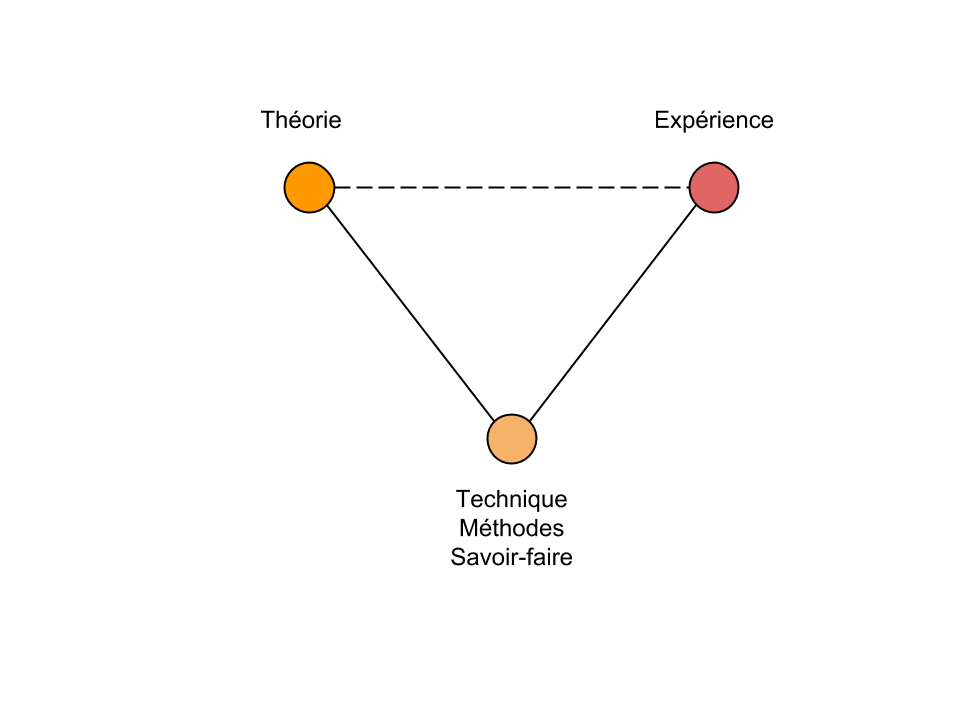
\includegraphics[width=5.0559in,height=3.7894in]{figures/chap3/chapitre3-img1.png}
    \caption[Triptyque des pratiques scientifiques]{Triptyque des pratiques scientifiques}
\end{figure}


En sciences humaines n\'eanmoins, la tension entre la th\'eorie (les
concepts), l{\textquoteright}exp\'erience (le terrain) et la
m\'ethodologie s{\textquoteright}articule plus rarement autour
d{\textquoteright}outillages \'elabor\'es. Les \ r\'eflexions sur la
m\'ethodologie en sciences sociales portent plus largement sur des
argumentations conceptuelles o\`u le langage lui-m\^eme est
consid\'er\'e comme l{\textquoteright}outil premier ou encore de
nombreuses r\'eflexions \'ethiques sur l{\textquoteright}impact des
pratiques d{\textquoteright}observation dans le cadre de
l{\textquoteright}anthropologie notamment. En France,
l{\textquoteright}int\'er\^et constant port\'e \`a
l{\textquoteright}utilisation des diff\'erentes formes de technologie
en sciences humaines s{\textquoteright}est souvent constitu\'e autour
de la critique de m\'ethodologies quantitatives tr\`es r\'epandues
outre atlantique - la statistique en sociologie,
l{\textquoteright}\'etude comportementaliste en psychologie ou le film
ethnographique \citep{Becker1974}. Comme le note justement Latour, la
qu\^ete de l\'egitimit\'e des Sciences Sociales s{\textquoteright}est
souvent traduit par une capacit\'e \`a se procurer et traiter des
donn\'ees : \textit{{\textquotedblleft}Sociology has been obsessed by
the goal of becoming a quantitative science.{\textquotedblright}}
\citep{Latour2010}. Pourtant, il serait illusoire de corr\'eler la
quantit\'e de donn\'ees \`a une quelconque objectivit\'e de la
d\'emarche scientifique, tant les d\'emarches et outils n\'ecessaires
pour la collecte sont en soi autant de biais importants. La question de
la r\'eussite des \'etudes utilisant les Big Data semblent davantage
corr\'el\'ee \`a la capacit\'e d{\textquoteright}une approche
m\'ethodologique forg\'ee dans un \'echange interdisciplinaire et des
pratiques renouvel\'ees de l{\textquoteright}\'ecriture. La
complexit\'e des questions abord\'ees lors du traitement des donn\'ees,
non seulement technologique mais aussi dans les interrogations sur la
l\'egitimit\'e de leur existence, leur utilisation et leur provenance
\citep{Boyd2011} rendent n\'ecessaire la discussion entre de
multiples connaissances. Aujourd{\textquoteright}hui,
l{\textquoteright}utilisation de l{\textquoteright}ordinateur
conditionne l{\textquoteright}\'ecriture scientifique de
l{\textquoteright}\'etude de terrain, la prise de notes, la r\'edaction
ou la publication et se pr\'esente ainsi comme un imp\'eratif
m\'ethodologique pour la r\'eflexion et le travail en sciences humaines
et sociales \citep{Wieviorka2013}. L{\textquoteright}appareillage projet\'e
au centre de la pratique quotidienne du chercheur vient modifier le
travail de r\'eflexion sur les ph\'enom\`enes \'etudi\'es et
s{\textquoteright}accompagne de multiples contraintes. La prise en main
de ce nouvel \textit{{\textquotedblleft}instrument
intellectuel{\textquotedblright} }\citep{Guichard2014} passe par une lente
alphab\'etisation aux langages des machines. L{\textquoteright}angoisse
latente du {\textquotedblleft}bug{\textquotedblright}
n{\textquoteright}est pas apais\'ee par les rares techniciens
pr\'esents dans les centres de recherche en sciences humaines, souvent
d\'ej\`a d\'epass\'es par la diversit\'e des demandes technologiques.
L{\textquoteright}\'ecriture, savoir-faire indispensable de la
recherche, poss\`ede une nouvelle mat\'erialit\'e dans les disques durs
produisant une d\'ependance accrue aux r\'eseaux
d{\textquoteright}ordinateurs. Cette empreinte
{\textquotedblleft}digitale{\textquotedblright} laiss\'ee par les
calculateurs sur les pratiques scientifiques n{\textquoteright}est ni
anodine ni r\'evolutionnaire et s{\textquoteright}inscrit dans la
longue tradition des cultures de l{\textquoteright}\'ecrit qui d\'ej\`a
bien avant les moines copistes \textit{{\textquotedblleft}combinent les
gestes de la main et les op\'erations de la
pens\'ee.{\textquotedblright}} \citep{Jacob2011} 

Tim Berners-Lee, consid\'er\'e comme l{\textquoteright}inventeur du
World Wide Web et du Web S\'emantique d\'efinit la constitution
d{\textquoteright}un r\'eseau mondial des savoirs comme un projet
d{\textquoteright}\textit{{\textquotedblleft}ing\'enierie
philosophique{\textquotedblright} }\citep{Halpin2014}.
Mi-philosophe mi-ing\'enieur, le chercheur contribuant \`a ce r\'eseau
de savoir doit donc \^etre en capacit\'e de conna\^itre les protocoles
et les langages pour y acc\'eder et s{\textquoteright}y mouvoir
ais\'ement. La m\'ethode scientifique s{\textquoteright}\'ecrit
notamment avec de nouvelles formulations (fonctions, algorithmes,
code...). Les donn\'ees g\'en\'er\'ees par les usages
d{\textquoteright}un nombre croissant de machines communicantes et
productrices d{\textquoteright}information, souvent d\'esign\'ees par
le concept {\guillemotleft}~valise~{\guillemotright} de Big Data \citep{Lohr2012} offrent des possibilit\'es nouvelles pour
l{\textquoteright}\'etude en sciences sociales.
L{\textquoteright}analyse de ces vastes jeux de donn\'ees
s{\textquoteright}accompagne \'egalement de nouveaux imp\'eratifs et
questionnements sur l{\textquoteright}observation des ph\'enom\`enes
humains qu{\textquoteright}ils repr\'esentent. \`A la fois barri\`ere
et opportunit\'e, une difficult\'e majeure r\'eside dans le
discernement n\'ecessaire entre praxis des outils informatiques,
fascination pour ces outils et r\'eflexions pertinentes sur la
qualit\'e des m\'ethodes employ\'ees. Le traitement quantitatif par
ordinateur permet d{\textquoteright}extraire de nombreuses
connaissances utiles de jeux de donn\'ees parfois tr\`es importants
mais n{\textquoteright}assure pas pour autant la qualit\'e des
r\'esultats. Une bonne compr\'ehension de la provenance et des
m\'ethodes de collection des donn\'ees est n\'ecessaire afin
d{\textquoteright}identifier des algorithmes de traitements
int\'eressants, adapt\'es et efficaces parmi ceux disponibles
\citep{Rajaraman2011}. Les m\'ethodologies
d{\textquoteright}exploration et de recherche utilisant le
{\textquotedblleft}Big Data{\textquotedblright} comme source
n\'ecessite la mise en {\oe}uvre d{\textquoteright}une ing\'enierie
complexe soutenu par une connaissance des technologies n\'ecessaires
\`a l{\textquoteright}analyse de donn\'ees.
L{\textquoteright}algorithmique, la statistique,
l{\textquoteright}informatique mais \'egalement la cartographie et le
design graphique doivent se conjuguer pour permettre de produire des
r\'esultats \`a la fois int\'eressants et fiables. Ce travail
d{\textquoteright}hypoth\`eses et de v\'erifications pour
l{\textquoteright}analyse de donn\'ees doit r\'eunir de nombreuses
comp\'etences. La d\'efinition de la probl\'ematique la plus adapt\'ee
n\'ecessite une connaissance aig\"ue du terrain et des outils et
algorithmes qui seront articul\'es au sein d{\textquoteright}un
syst\`eme ing\'enierique parfois tr\`es complexe. Le design et la
lecture d{\textquoteright}algorithme pour le
\textit{{\textquotedblleft}data mining{\textquotedblleft}} sont donc
les cl\'es pour le travail du chercheur confront\'e aux donn\'ees.
N\'eanmoins, ces algorithmes ne devraient \^etre que la traduction de
questions formul\'ees gr\^ace \`a une connaissance aig\"ue des
probl\'ematiques du contexte et des objets \'etudi\'es - notamment pour
identifier les donn\'ees manquantes. La {\textquotedblleft}science des
donn\'ees{\textquotedblright} promet donc d{\textquoteright}apporter un
v\'eritable renouveau des m\'ethodes et des r\'esultats scientifiques,
au prix d{\textquoteright}un travail soutenu pour faire face \`a ces
changements d{\textquoteright}habitudes et de langages. Les
applications statistiques du {\textquotedblleft}big
data{\textquotedblright} permettent aujourd{\textquoteright}hui une
fiabilit\'e accrue des pr\'edictions par l{\textquoteright}augmentation
du volume des corpus trait\'es \citep{Breiman2001}. Le domaine de
l{\textquoteright}intelligence artificielle (AI) a grandement
b\'en\'efici\'e de l{\textquoteright}accroissement de la capacit\'e de
traitement des donn\'ees notamment pour la pr\'ediction gr\^ace au
techniques dites de \textit{machine learning}. N\'eanmoins Peter
Norvig, directeur de recherche chez Google, reconnait lui-m\^eme :
{\textquotedblleft}\textit{We could draw this curve: as we gain more
data, how much better does our system get? And the answer is,
it{\textquoteright}s still improving---but we are getting to the point
where we get less benefit than we did in the past.{\textquotedblright}
}\citep{Somers2013}. Comme le note Douglas Hofstadter, un des pairs de
l{\textquoteright}Intelligence Artificielle \`a propos du
super-ordinateur qui venait de battre Kasparov aux \'echecs :
\textit{{\textquotedblleft}Okay, Deep Blue plays very good chess---so
what? Does that tell you something about how we play chess? No. Does it
tell you about how Kasparov envisions, understands a
chessboard?{\textquotedblright} }\citep{Somers2013}. 

En effet, ces pratiques m\'ethodologiques doivent r\'eussir \`a
s{\textquoteright}inscrire dans la continuit\'e de
l{\textquoteright}historicit\'e et des exigences des disciplines. La
portabilit\'e des m\'ethodes et la disponibilit\'e des donn\'ees sont
encore des questions centrales et non-r\'esolues. En sciences sociales
notamment, les services de r\'eseaux sociaux en ligne offrent de tr\`es
large corpus dont l{\textquoteright}utilisation est r\'egie par les
exigences commerciales des soci\'et\'es priv\'ees qui les d\'etiennent.
L{\textquoteright}analyse des donn\'ees issues de service de r\'eseaux
sociaux en ligne est pourtant un champ d{\textquoteright}\'etudes en
rapide expansion \citep{Nettleton2013}. Pourtant, le d\'ebat sur la
validit\'e des \'eclairages apport\'es par l{\textquoteright}analyse
des donn\'ees issues des services de r\'eseaux reste encore largement
ouvert et nous entendons dans ce travail de recherche y contribuer. 

\subsection[Visualisation et espace perceptif pour l{\textquoteright}information]{3.1.3 Visualisation et espace perceptif pour l{\textquoteright}information}
Face \`a de larges volumes de donn\'ees, un des grands enjeux est
d{\textquoteright}en restituer une forme intelligible afin de
d{\textquoteright}identifier des tendances ou des motifs particuliers.
La visualisation permet de produire une lecture particuli\`ere de
parties int\'eressantes et intelligibles d{\textquoteright}un jeu de
donn\'ees \citep{Cairo2013}. D\'efinie comme \textit{{\guillemotleft}~a
process that transforms data, information, and knowledge into a form
that relies on the human visual system to perceive its embedded
information.{\textquotedblright}} \citep{Graffieti2010}, la
visualisation introduit la question du design visuel au c{\oe}ur de la
probl\'ematique d{\textquoteright}analyse \citep{Wesolowsky1992}.
La visualisation correspond \`a une s\'erie d{\textquoteright}actions
qui r\'esulte dans la production de marqueurs visuels (points, ligne,
aires, surface, volume) avec comme \'etapes la d\'efinition de leurs
propri\'et\'es r\'etiniennes (couleur, taille, texture, etc.) et leur
positionnement dans l{\textquoteright}espace visuel \citep{Card Mackinlay}
 \`a d\'efinir les bases d{\textquoteright}une grammaire de la
visualisation en commen\c{c}ant par en identifier les formes
syntaxiques : 

\begin{enumerate}
\item les objets graphiques montr\'es (ex. point, fl\`eche, pictogramme,
etc.), 
\item l{\textquoteright}espace graphique donnant sens \`a
l{\textquoteright}organisation des objets (ex. syst\`emes de
coordonnn\'ees g\'eographiques, timeline, etc.),
\item les propri\'et\'es graphiques des objets (couleurs, tailles,
etc.),
\item l{\textquoteright}organisation des objets en diff\'erentes
cat\'egories~(ex. cadre, liens, l\'egendes, etc.). 
\end{enumerate}
Ces choix forment une t\^ache importante dont l{\textquoteright}enjeu
n{\textquoteright}est pas seulement visuel, mais se joue \'egalement
dans le champ de la repr\'esentation o\`u les objets sont donn\'es \`a
voir et par l\`a-m\^eme donn\'es \`a comprendre. Les travaux sur
l{\textquoteright}apparition de la perspective dans la Renaissance
italienne ont montr\'e comment l{\textquoteright}espace de la
repr\'esentation visuelle fait \'echo aux changements soci\'etaux
profonds de l{\textquoteright}\'epoque \citep{Raynaud2005}. Au-del\`a
d{\textquoteright}une simple technique picturale, les {\oe}uvres des
peintres du Quattrecento t\'emoignent de changements profonds dans la
perception : l{\textquoteright}espace perceptif se structure
d\'esormais autour du sujet et \ de son {\textquotedblleft}point de
vue{\textquotedblright} qui construit l{\textquoteright}ensemble de la
repr\'esentation \citep{Damisch1999}. Empreinte de rationalit\'e, la
perspective construit comme au th\'e\^atre un espace de
repr\'esentation centr\'e autour du spectateur. En 1639, le
math\'ematicien Desargues mod\'elise les notions intuitives de
perspective et d{\textquotesingle}horizon gr\^ace \`a la g\'eom\'etrie
projective qui permet d{\textquoteright}\'etudier les propri\'et\'es
inchang\'ees des figures lors de leur projection. Cette g\'eom\'etrie
d{\textquoteright}un genre nouveau se structure autour du \textit{plan
projectif}, \'el\'ement topologique qui
\textit{{\textquotedblleft}rassemble en une seule surface
l{\textquoteright}imagination de tous les points de vue
possible{\textquotedblright} }\citep{Petit1996}. En construisant un plan
g\'eom\'etrique fond\'e sur le point de vue, de nouveaux \^etres
g\'eom\'etriques aux propri\'et\'es \'etranges voient le jour, dont
l{\textquoteright}existence logique force notre repr\'esentation
classique : la bande de M\"obius ne poss\`ede qu{\textquoteright}une
seule face et il est impossible de distinguer
l{\textquoteright}int\'erieur de l{\textquoteright}ext\'erieur
d{\textquoteright}une bouteille de Klein. Dans ces surfaces dites
\textit{unilat\`eres}, le local est travers\'e en tout point par un
tout global. Nous ne pouvons pas traverser puisque nous somme toujours
sur la m\^eme face. Ni bord, ni ext\'erieur, ni int\'erieur, le plan
projectif apporte des \'el\'ements de r\'eponses conceptuelles aux
limites des la repr\'esentation dans l{\textquoteright}espace. 

Dans le contexte de syst\`emes et de r\'eseaux complexes, la
visualisation de donn\'ees structure l{\textquoteright}espace perceptif
afin de construire une sc\`ene \`a \textit{n }dimensions dont
l{\textquoteright}enjeu est la recherche d{\textquoteright}un
{\textquotedblleft}point de vue{\textquotedblright} pour
l{\textquoteright}\'etude\textit{. }Alors que la perspective prend pour
parti de mat\'erialiser le sujet au centre de la repr\'esentation par
des points de fuite, la visualisation de donn\'ees cherche elle \`a
utiliser les objets comme dimensions du champ de la repr\'esentation,
en structurant souvent l{\textquoteright}espace autour de quantit\'es.
N\'eanmoins, la place du spectateur / utilisateur dans la visualisation
reste un des enjeux majeurs encore \`a explorer. En \'elaborant sa
{\textquotedblleft}m\'ethode graphique{\textquotedblright} , J.E. Marey
\citep{Marey1885} utilise la photographie pour cr\'eer un nouvel espace de
repr\'esentation du mouvement et observer des ph\'enom\`enes
jusqu{\textquoteright}ici invisibles. Si la temporalit\'e de
l{\textquoteright}\'ecrit ou de la voix est avant lin\'eaire,
l{\textquoteright}espace visuel permet de manier le r\'eel pour le
d\'ecomposer en actes logiques. Charcot cherche dans les images de
l{\textquoteright}hyst\'erie des t\'emoignages de la folie et proc\`ede
\`a la mise en sc\`ene de ses patients dans ce nouvel espace de
repr\'esentation ouvert par la photographie \citep{Didi-Huberman2012}.

La visualisation scientifique se pr\'evaut donc d{\textquoteright}une
existence avant tout pratique dont le premier objectif serait de
\textit{{\guillemotleft}~to effectively convey
information~{\guillemotright}} \citep{Kelleher2011}. Son
caract\`ere syncr\'etique et sa capacit\'e \`a r\'esumer une large
masse d{\textquoteright}information rapidement en font un des plus
importants \'el\'ements de la publication en science notamment pour sa
diffusion et la facilitation d{\textquoteright}acc\`es \`a une
connaissance \citep{Ware2004}. Dans sa s\'emiologie graphique, Bertin
\citep{Bertin1977} distingue deux usages majeurs des graphiques de visualisation :
1) un moyen de communiquer des informations (dans le cas o\`u
l{\textquoteright}information a d\'ej\`a \'et\'e comprise) 2) un moyen
visuel de r\'esoudre des probl\`emes logiques (quand le graphique est
utilis\'e comme support de lecture et de manipulation
d{\textquoteright}informations). Ces deux caract\'eristiques peuvent
coexister dans certaines pi\`eces mais la transition entre les deux
n\'ecessite souvent un travail important de restructuration visuelle.
Dans le traitement et la la visualisation des donn\'ees
\textit{l{\textquoteright}interface }joue un r\^ole primordial. On peut
d\'esormais agir sur la 2\`eme cat\'egorie de Bertin pour mieux
explorer le sens \citep{Weissberg2007}. Manovich montre comment
l{\textquoteright}interface d\'efinie comme
\textit{{\textquotedblleft}the ways to represent
({\textquoteleft}format{\textquoteright}) and control the
signal.}{\textquotedblright} \citep{Manovich2013}. Ce formatage nouveau de
l{\textquoteright}information induit des changements dans la pratique
de la lecture qui, toujours selon Manovich,
s{\textquoteright}apparenterait davantage \`a de la reconnaissance de
\textit{pattern}, symbolis\'e par l{\textquoteright}usage de
l{\textquoteright}ic\^one et du menu en design
d{\textquoteright}interface. Ainsi si l{\textquoteright}interface
contraint la lecture, la prise en compte des formes narratives (les
\textit{patterns} de Manovich) prend une grande importance quand il
s{\textquoteright}agit de concevoir une visualisation
d{\textquoteright}information. L{\textquoteright}usage des signes
graphiques doit se faire avec une connaissance des usages de
l{\textquoteright}interface, afin de recr\'eer la coop\'eration
textuelle des r\^oles de lecteur et de designer/auteur n\'ecessaire
pour la production un sens \citep{Eco1985}. La \textit{citizen science} ou
encore \textit{night science} a fait de l{\textquoteright}interface un
paradigme en utilisant la visualisation pour amener un grand nombre de
collaborateurs \`a explorer et analyser de vastes jeux de donn\'ees en
effectuant des t\^aches simples \citep{Silvertown2009}. Le projet
\textit{Eyewire} permet \`a des internautes de contribuer \`a la
classification d{\textquoteright}images du cerveau humain en vue de la
r\'ealisation d{\textquoteright}un mod\`ele 3D \citep{Seung2012}. Utilisant
des scans de tranches de 1mm r\'ealis\'es par
l{\textquoteright}institut Max Planck, la mod\'elisation 3D
d{\textquoteright}un cerveau complet promet une belle contribution pour
la d\'ecouverte des fonctionnements cognitifs. N\'eanmoins, la t\^ache
est colossale et n\'ecessiterait plusieurs ann\'ees pour une \'equipe
classique de scientifiques. \textit{Eyewire} propose donc une interface
web o\`u un simple jeu de coloriage permet d{\textquoteright}identifier
les neurones et de contribuer ainsi au dessin du mod\`ele 3D.

Cartes, code ou graphiques, les nouveaux outils num\'eriques participent
donc \`a structurer de nouvelles pratiques de l{\textquoteright}espace
gr\^ace \`a la construction de nouvelles repr\'esentations. 

\section[M\'ethodes et outils d{\textquoteright}analyse des r\'eseaux sociaux]{M\'ethodes et outils d{\textquoteright}analyse des r\'eseaux sociaux}

Nous allons maintenant regarder comment l{\textquoteright}analyse des
donn\'ees des services de r\'eseaux sociaux en ligne (SNA) peut
permettre d{\textquotesingle}interroger les pratiques des technologies
num\'eriques pour mieux en comprendre les tenants.

\subsection[Anatomie d{\textquoteright}un r\'eseau social]{ Anatomie d{\textquoteright}un r\'eseau social}
La repr\'esentation des relations sociales sous forme de graphe trouve
son origine dans les travaux des psychologues allemands de la
\textit{gestalt }durant les ann\'ees 1920-1930 \citep{Scott1988}\textit{.
}S{\textquoteright}inspirant des \'etudes sur le cerveau, le
psychologue J. L. Moreno s{\textquoteright}applique notamment \`a
comprendre les principes organisationnels holistiques des groupes
humains et fonde la sociom\'etrie avec comme objectif la qualification
et la quantification des relations sociales \citep{Moreno1938}.
Moreno cherche \`a identifier et isoler des leaders de groupes sociaux
d\'efinis en \'etudiant l{\textquoteright}asym\'etrie ou la
r\'eciprocit\'e de leurs choix et fr\'equentations amicales. Cherchant
des moyens de repr\'esenter les tendances \`a
l{\textquoteright}auto-organisation qu{\textquoteright}il observe, il
cartographie les relations directes et indirectes entre personnes sous
forme de \textit{sociogrammes}. Les anthropologues
s{\textquoteright}emparent rapidement de ce type
d{\textquoteright}outils pour comprendre les formes tribales (Lundberg,
1936) et l{\textquoteright}\'emergence progressive de la topologie
comme domaine important des math\'ematiques vient d\'efinir de nouveaux
types de relations entre objets disparates, avec notamment la th\'eorie
des graphes qui donne \`a l{\textquoteright}\'etude des r\'eseaux ses
mod\`eles logiques \citep{Harary1977}. Milgram \citep{Milgram1969} voit les relations
humaines comme autant de petits mondes (\textit{small-worlds)}
connect\'es entre eux. Granovetter s{\textquoteright}int\'eresse \`a
l{\textquoteright}importance des relations t\'enues et lointaines
(\textit{weak ties}) dans l{\textquoteright}acquisition
d{\textquoteright}informations importantes \citep{Granovetter1974}.
L{\textquoteright}influence de la th\'eorie des graphes am\`ene
notamment les sociologues \`a exp\'erimenter de nouveaux mod\`eles
venus de la physique ou de la biologie, en proposant de nouvelles
pratiques comme celle de la simulation sociale \citep{Epstein1996}.



La mat\'erialit\'e de l{\textquoteright}image du \textit{graphe}
structure la repr\'esentation du r\'eseau social. Dans la litt\'erature
concernant les r\'eseaux, les notions de graphe et de r\'eseau sont
interd\'ependantes et la th\'eorie des graphes sert notamment de
syst\`emes de notation pour la mise en \'equation des r\'eseaux
\citep{Nettleton2013}. Si cette structure point-ligne semble toutefois
rev\^etir une limite de taille pour la description de ph\'enom\`enes
humains (comment en effet r\'eduire les relations humaines \`a une
simple ligne?), elle semble n\'eanmoins aujourd{\textquoteright}hui
encore difficile \`a d\'epasser.

\begin{figure}
    \centering
    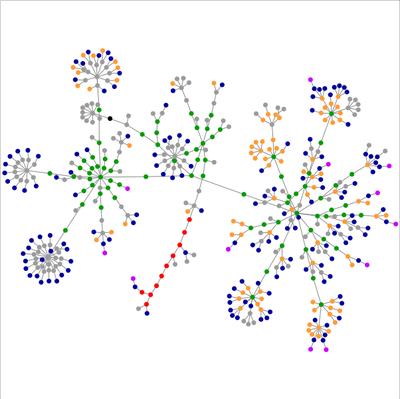
\includegraphics[width=4.178in,height=4.1449in]{figures/chap3/chapitre3-img2.png}
    \caption{Représentation d'un r\'eseau sous forme de graphes.}
\end{figure}


Un r\'eseau consid\'er\'e comme graphe, not\'e \textit{G}, se compose
d{\textquoteright}un ensemble de nodes ou vertices (les points) et de
liens ou edges (les traits). On repr\'esente ainsi un graphe sous la
notation \textit{G(V,E)} o\`u \textit{V }est l{\textquoteright}ensemble
des nodes du r\'eseau et \textit{E} l{\textquoteright}ensemble des
liens\textit{ }d\'ecrivant leurs relations. \textit{E }d\'ecrit les
relations entre les nodes qui peuvent \^etre directionnelles (paires de
vertices ordonn\'ees) dans le cas d{\textquoteright}un graphe
\textit{orient\'e }ou accompagn\'e de valeurs particuli\`eres dans un
graphe dit \textit{pond\'er\'e. }Les relations ainsi exprim\'ees
portent sur un aspect unique, quantifiable et isolable. La prise en
compte de facteurs multiples, comme notamment l{\textquoteright}espace
physique, le temps, mais \'egalement les multiples r\'eseaux de
relations qui peuvent exister entre deux acteurs nous am\`enent \`a
consid\'erer un graphe disposant de multiples couches
\textit{(}\textit{multi-layered)} pour d\'ecrire
l{\textquoteright}ensemble des groupes de relations. Imaginons un
graphe de personnes \textit{G (V,E}\textit{\textsubscript{n}}\textit{)} o\`u \textit{V }sont les
vertices repr\'esentant les personnes et \textit{E}\textsubscript{n} un
nombre \textit{n }d{\textquoteright}ensemble de liens\textit{
}d\'ecrivant chaque type de relations sp\'ecifiques. Le graphe
ci-dessous montre un exemple d{\textquoteright}un graphe multi-couche
o\`u \textit{E}\textit{\textsubscript{1}} est
l{\textquoteright}ensemble des relations amicales,
\textit{E}\textit{\textsubscript{2}}\textsubscript{ }les relations de
travail et \textit{E}\textit{\textsubscript{3}}\textsubscript{ }les
relations familiales.

\begin{figure}
    \centering
    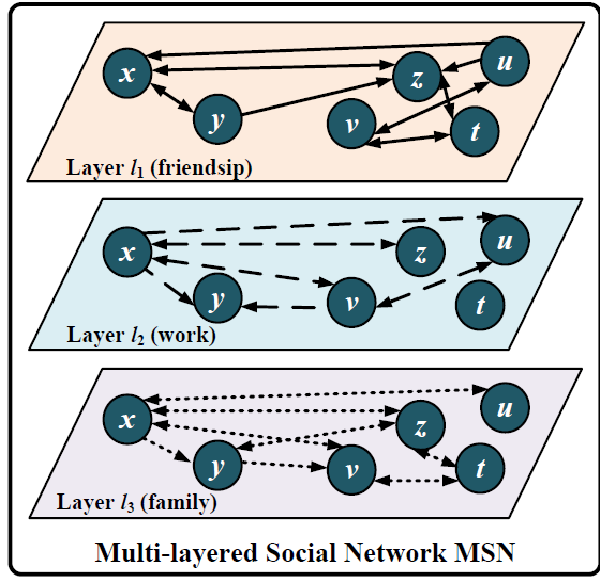
\includegraphics[width=3.8004in,height=3.6894in]{figures/chap3/chapitre3-img3.png}
    \caption [r\'eseau social multi-couches] {Un r\'eseau social multi-couches, d{\textquoteright}apr\`es (Brodka\&al., 2013)}
\end{figure}

Nous pouvons ainsi d\'ecrire diff\'erents jeux de relations entre un jeu
d{\textquoteright}acteurs finis, permettant notamment de mieux
comprendre les relations entre ses diff\'erentes dimensions. Si cette
approche r\'esout momentan\'ement la question des \textit{n }dimensions
\`a consid\'erer \citep{Br\'odka2013} elle augmente \'egalement la
complexit\'e du graphe et la possibilit\'e d{\textquoteright}erreurs de
lecture ou de typage des relations. 

Afin de mieux comprendre l{\textquoteright}organisation
d{\textquoteright}un r\'eseau, nous disposons de plusieurs mesures~pour
d\'ecrire les relations et le r\^ole des diff\'erents acteurs : 
i
\begin{itemize}
\item \textit{Degree} : (\textit{degr\'e} ou \textit{valence}) mesure le
nombre de connections d{\textquoteright}un n{\oe}ud dans un r\'eseau.
Cette valeur indique souvent une possibilit\'e, le potentiel
d{\textquoteright}un node donn\'e \`a interagir avec
d{\textquoteright}autres. 
\item \textit{Closeness : }(proximit\'e) mesure la facilit\'e
d{\textquoteright}un node \`a se connecter \`a un autre. Dans un
r\'eseau en ligne, on calcule la proximit\'e en estimant la distance la
plus courte entre un node et un autre. 
\item \textit{Betweenness} (\textit{centralit\'e}) mesure le degr\'e
d{\textquoteright}importance d{\textquoteright}un node dans le r\'eseau
en prenant en compte le nombre de nodes d\'ependant de lui pour
\'etablir une connection entre eux. La centralit\'e repr\'esente la
capacit\'e \`a bloquer ou laisser filtrer l{\textquoteright}acc\`es \`a
certaines parties du r\'eseau. Dans une entreprise par exemple, la
secr\'etaire du CEO a par exemple une tr\`es haute centralit\'e.
\end{itemize}


En observant ces diff\'erentes mesures, nous pouvons d\'efinir
diff\'erentes structures types pour chaque r\'eseau. La distribution
des degr\'es dans le graphe permet notamment de comprendre les
mod\`eles qui r\'egissent les connexions entre les nodes.
L{\textquoteright}exemple le plus simple est le \textit{random network,
}r\'eseau o\`u les acteurs sont connect\'es de mani\`ere enti\`erement
al\'eatoire. Un r\'eseau dont le degr\'e de distribution correspond \`a
une loi de puissance est appel\'e \textit{scale-free network. }Un
r\'eseau dont seulement quelques nodes poss\`edent une centralit\'e
\'elev\'ee et dont la structure d{\textquoteright}ensemble est faite de
groupes ou \textit{clusters} interconnect\'es et appel\'e un
\textit{small-world network. }


\begin{figure}
    \centering
    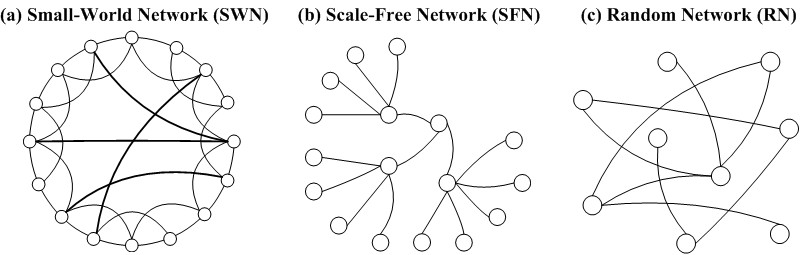
\includegraphics[width=6.3449in,height=2.0224in]{figures/chap3/chapitre3-img4.jpg}
    \centering{Types communs de r\'eseaux}
\end{figure}

Les services de r\'eseaux sociaux en ligne sont structur\'es en
\textit{small-worlds}. Dans une \'etude analysant de larges corpus
issus de diff\'erents services de r\'eseaux sociaux en ligne, Kumar \&
al. \citep{Kumar2006} ont montr\'e que ces communaut\'es poss\`edent toutes une
structure et une \'evolution similaire. Les inscrits de chaque service
se r\'epartissent autour de trois grands groupes : \textit{singletons}
(membres isol\'es, inactifs), \textit{giant component} (la majorit\'e
des utilisateurs actifs) et \textit{middle region} (des communaut\'es
isol\'ees qui interagissent entre elles mais pas avec le reste du
r\'eseau). D{\textquoteright}apr\`es les auteurs, il existe tr\`es peu
de chances que deux communaut\'es isol\'ees m\^eme tr\`es similaires se
rencontrent dans ce type de r\'eseau, car l{\textquoteright}entropie de
la structure \textit{small-world }se renforce avec le temps en se
fragmentant davantage. Une des raisons principales est que ces
communaut\'es isol\'ees suivent souvent un mod\`ele en
\textit{\'etoile, }c{\textquoteright}est \`a dire
qu{\textquoteright}elles sont construites autour d{\textquoteright}un
individu central charismatique. \'Eventuellement, il leur arrive de
rejoindre la masse du \textit{giant component} mais elles en deviennent
difficilement des acteurs majeurs et restent en p\'eriph\'erie. Dans un
r\'eseau social de type small-world comme les OSNS, les acteurs les
plus influents sont ceux qui sont capables de 1) renforcer les liens
dans un cluster (\textit{closure)} et 2) d\'evelopper les connections
faibles entre des clusters (\textit{brokerage)} (Burt, Centola, \&
Kahl, 2008). Ce {\textquotedblleft}capital social{\textquotedblright}
est inscrit dans la structure du r\'eseau social lui-m\^eme \citep{Lin1999}
et n{\textquoteright}a pas de relations avec le degr\'e du node (son
nombre de connections) \citep{Cha2010}. L{\textquoteright}individu
le plus puissant d{\textquoteright}un r\'eseau est donc celui
poss\'edant le plus grand nombre de connections \textit{potentielles,
}proches et facilement accessibles et qui b\'en\'eficie
d{\textquoteright}une place privil\'egi\'ee pour bloquer ou autoriser
l{\textquoteright}acc\`es aux autres parties du r\'eseau.
L{\textquoteright}analyse organisationnelle a notamment montr\'e
l{\textquoteright}importance capitale des secr\'etaires pour le
maintien d{\textquoteright}une bonne circulation des informations dans
le r\'eseau de l{\textquoteright}entreprise ou la n\'ecessit\'e
d{\textquoteright}un nombre tr\`es faible de connections directes pour
les acteurs importants de r\'eseaux terroristes ou mafieux \citep{Russel2011}. 

\subsection[Diffusion des discours dans les r\'eseaux sociaux]{Diffusion des discours dans les r\'eseaux sociaux}
L{\textquoteright}analyse de r\'eseau social permet de comprendre la
structure d{\textquoteright}un moment du r\'eseau. En effet, les
connections entre diff\'erents acteurs sont sans cesse en mouvement et
l{\textquoteright}information en circulant vient modifier
l{\textquoteright}activit\'e du r\'eseau et bien souvent sa structure
m\^eme. Notre \'etude porte sur la diffusion de m\`emes au sein du
r\'eseau social chinois Sina Weibo et s{\textquoteright}inscrit ainsi
dans la continuit\'e des travaux s{\textquoteright}int\'eressant aux
rapports entre diffusion et technologies. N\'eanmoins, le champ de la
diffusion de l{\textquoteright}innovation, objet traditionnel de la
g\'eographie, s{\textquoteright}est largement constitu\'e autour des
probl\'ematiques technologiques et organisationnelles li\'ees \`a la
situation spatiale du lieu et ses \'equipements \citep{Crevoisier2004}. Les
\'etudes urbaines ont notamment montr\'e comment la r\'ealit\'e
\'economique et g\'eographique pr\'esidait \`a la constitution des
savoirs n\'ecessaires \`a la diffusion de l{\textquoteright}innovation
technologique \citep{Howells2002}. Cette vision doit \^etre mod\'er\'ee par
une consid\'eration plus importante des modalit\'es
d{\textquoteright}appropriation des technologies comme pratiques
propres aux territoires \citep{Fernandez2010}. Plus largement, les
\'etudes sur la diffusion sont domin\'ees par
l{\textquoteright}analogie du virus comme mod\`ele de propagation des
messages, comportements et id\'ees. Depuis la fin du XIXe si\`ecle (Le
Bon, 1895), ce mod\`ele est pr\'epond\'erant dans les recherches autour
de la diffusion d{\textquoteright}information en ligne \citep{Goel2012} Les membres de groupes dans un r\'eseau seraient
\textit{expos\'es }\`a un message ou une id\'ee avant
d{\textquoteright}\^etre \textit{infect\'es, }devenant alors porteur
puis agent de sa diffusion. Ainsi, en consid\'erant la position
d{\textquoteright}un individu au sein du r\'eseau de diffusion, il
serait possible de d\'efinir un
\textit{{\textquotedblleft}}\textit{degr\'e
d{\textquoteright}infection{\textquotedblright}} \citep{Cheng et al.2013}
et d{\textquoteright}anticiper la diffusion selon une
\textit{{\guillemotleft}~probabilit\'e immune~{\guillemotright}
}qui\textit{ }d\'eciderait de la \textit{{\guillemotleft}~qualit\'e
infectieuse~{\guillemotright} }de l{\textquoteright}objet diffus\'e ou
de la \textit{{\guillemotleft}~possibilit\'e de
}\textit{r\'etablissement~{\guillemotright} }du sujet infect\'e \citep{Wang2011}. Cette analogie du viral propose une vision
m\'ecaniste qui fait peu de cas des facteurs contextuels ou
psychologiques et ignorent ainsi les processus de d\'ecisions
individuels en jeu \citep{Jackson2010}. Pourtant, nous savons
notamment que le choix des mots ou la situation des personnes diffusant
un message sont des facteurs d\'ecisifs et structurant des processus
d{\textquoteright}adoption des messages en ligne \citep{Conover2013}. 
En s{\textquoteright}int\'eressant \`a la diffusion
g\'eographique de mots dans les r\'eseaux sociaux, Eisenstein \& al.
\citep{Eisenstein2012} observe que leur diffusion se limite \`a un domaine
g\'eographiquement bien d\'efini, d\'ependant de facteurs culturels et
d\'emographiques. Par exemple, les villes ayant
d{\textquoteright}importantes communaut\'es afro-am\'ericaines ont
davantage de chances d{\textquoteright}adopter un m\^eme mot que
d{\textquoteright}autres parfois plus proches g\'eographiquement. Cette
question est au centre des \'etudes de marketing qui
s{\textquoteright}interrogent notamment sur l{\textquoteright}adoption
de nouvelles marques ou de slogans. Afin de d\'eterminer
statistiquement les possibilit\'es d{\textquoteright}adoption de
produits et pr\'evoir la p\'en\'etration dans un march\'e pr\'ecis, la
mod\'elisation math\'ematique des effets de r\'eseaux dans la diffusion
est souvent utilis\'e \citep{Bass1994}. Ici,
l{\textquoteright}analyse des donn\'ees des r\'eseaux sociaux est un
grand enjeu pour la prospective \'economique et
l{\textquoteright}application de ces mod\`eles math\'ematiques aux
donn\'ees utilisateurs permettant de consid\'erer des segments pr\'ecis
de march\'e. Le marketing politique fait lui aussi grand cas de
l{\textquoteright}analyse de r\'eseaux sociaux pour comprendre et
orienter les discussions. La campagne de r\'e\'election
d{\textquoteright}Obama aux USA en 2012 a fait un usage extensif de
l{\textquoteright}analyse de donn\'ees des r\'eseaux sociaux pour
identifier, d\'eterminer et cibler des groupes sociaux particuliers
gr\^ace au travail d{\textquoteright}une vaste \'equipe
d{\textquoteright}ing\'enieurs et de \textit{{\textquotedblleft}data
scientists{\textquotedblright}}\footnote{
\textit{{\textquotedblleft}Harper Reed, the chief technology officer
for the Obama re-election campaign, who heads a team described as
{\textquotedblleft}100 data scientists, developers, engineers,
analysts, and old-school hackers [that] have been transforming the way
politicians acquire data---and what they do with
it.{\textquotedblright}, }from \ The Blaze
\url{http://www.theblaze.com/stories/2012/10/03/very-creepy-details-of-obama-campaigns-voter-data-mining-effort/}
consult\'e le 12 Mars 2014 \`a 14:50 GMT+1}\textit{. }

Une des grandes interrogations dans ce domaine est \'evidemment les
r\^oles jou\'es par les diff\'erents acteurs du processus de diffusion
-- et la mani\`ere de les identifier. Les \'etudes concernant les
leaders d{\textquoteright}opinion, traditionnelles en sciences de la
communication \citep{Katz1955} trouvent une continuit\'e
directe dans l{\textquoteright}\'etude des r\'eseaux sociaux en ligne
avec le domaine florissant des recherches sur
l{\textquoteright}identification des \textit{influenceurs} \citep{Bakshy2011, Leavitt2009}. L{\textquoteright}analyse quantitative permet notamment de mieux
comprendre l{\textquoteright}influence r\'eelle des acteurs dans le
r\'eseau gr\^ace \`a l{\textquoteright}\'etude de leurs comportements.
Le concept d{\textquoteright}influence sur les r\'eseaux sociaux
rev\^et en r\'ealit\'e des formes tr\`es variables et proc\`ede
notamment d{\textquoteright}une l\'egitimit\'e construite autour de
sujets pr\'ecis par \ des personnes sp\'ecialis\'ees devenues
r\'ef\'erentes \citep{Cha2010}. D{\textquoteright}autres
{\textquotedblleft}influenceurs{\textquotedblright} poss\`edent une
grande capacit\'e d{\textquoteright}amplification pouvant par exemple
initier le d\'eveloppement d{\textquoteright}une
\textit{{\textquotedblleft}masse critique{\textquotedblright} }autour
d{\textquoteright}une information\textit{, }d\'efinie classiquement
comme le seuil d{\textquoteright}adoption \`a partir duquel la
diffusion devient p\'erenne parmi une foule d{\textquoteright}acteurs
\citep{Oliver2001}. L{\textquoteright}image quantitative
d{\textquoteright}une {\textquotedblleft}masse{\textquotedblright}
uniforme et actionnable dans le r\'eseau est n\'eanmoins remise en
question par l{\textquoteright}\'etude de donn\'ees dont
l{\textquoteright}analyse montre que les relations entre diff\'erents
acteurs du r\'eseau sont \`a consid\'erer qualitativement en termes de
relations de pouvoirs \citep{Steyer2006}\textit{. }Les dynamiques
d{\textquoteright}\'echanges ne r\'epondent en effet pas tant \`a une
relation pr\'e-existente dans le r\'eseau qu{\textquoteright}\`a un
ensemble de situations o\`u les acteurs adoptent des comportements et
des r\'eactions particuli\`eres. La diffusion peut ainsi se comprendre
comme une pratique du \textit{bouche-\`a-oreille} \'eminemment
contextuelle, o\`u certains acteurs sont plus ou moins influents dans
telle ou telle situation ou sur tel et tel sujet. Le temps joue
n\'eanmoins un r\^ole d\'eterminant puisqu{\textquoteright}en
consid\'erant des s\'eries de r\'esultats o\`u des acteurs se
c\^otoient durant plusieurs ann\'ees, il est souvent difficile
d{\textquoteright}identifier quel acteur influence
l{\textquoteright}autre \citep{Aral2009}. 

\subsection[M\'ethodes d{\textquoteright}analyse de donn\'ees des r\'eseaux sociaux en ligne]{3.2.3. M\'ethodes d{\textquoteright}analyse de donn\'ees des r\'eseaux sociaux en ligne}
Apr\`es moins d{\textquoteright}un si\`ecle d{\textquoteright}existence,
l{\textquoteright}analyse de r\'eseaux sociaux sous forme de graphes a
donc connu une rapide \'evolution et une diversification dans de
nombreux domaines de recherche. Les services de r\'eseaux sociaux en
ligne offrent notamment la possibilit\'e d{\textquoteright}obtenir des
donn\'ees sur les comportements de groupes sociaux en tr\`es vaste
quantit\'e. V\'eritable vivier d{\textquoteright}\'etudes, ce champ de
recherche en pleine expansion trouve ses origines dans des disciplines
diverses qui poursuivent souvent des objectifs et des m\'ethodes tr\`es
diff\'erentes. Le tableau infra pr\'esente quelques-unes des m\'ethodes
d{\textquoteright}analyse de donn\'ees d\'efinies selon leurs domaines
d{\textquoteright}application. Ces m\'ethodes coexistent souvent lors
d{\textquoteright}\'etudes utilisant le \textit{data mining} ; nous
pr\'esentons ici des exemples qui permettront ensuite de mieux situer
nos perspectives de recherche~dans ce paysage de pratiques.



\begin{figure}
    \centering
\caption[Tableau r\'ecapitulatif de m\'ethodes d{\textquoteright}analyse de donn\'ees de r\'eseaux sociaux en ligne.]{Tableau r\'ecapitulatif de m\'ethodes d{\textquoteright}analyse de donn\'ees de r\'eseaux sociaux en ligne.}

\begin{tabular}{c|c|c|c|c}

&
\textbf{Courant d{\textquoteright}analyse} &
\textbf{M\'ethodologie} &
\textbf{Exemples d{\textquoteright}usages et applications} &
\textbf{Auteurs \& Publications de r\'ef\'erence}\\

1 &
Graphes sociaux de groupe d\'efinis (cartographie de r\'eseau fini) &
En partant d{\textquoteright}un \'echantillon fini et d\'etermin\'e au pr\'ealable, on effectue une carte des relations entre les diff\'erents acteurs du r\'eseau.  &

Cartographier les connections d{\textquoteright}apr\`es un profil sur un service de r\'eseau social en ligne  &
Cette pratique est l{\textquoteright}origine de la sociom\'etrie (Moreno \& Jennings, 1938) et de l{\textquoteright}\'etude des relatons sociales en tant que r\'eseaux.
\\

2 &
D\'ecouverte de groupes par crit\`eres (communaut\'es)

~
 &
Cette m\'ethode permet de r\'ealiser un \'echantillonnage
d{\textquoteright}un r\'eseau social \`a partir d{\textquoteright}un
ensemble de profils existants appel\'es \textit{seeds}. Un logiciel
(appel\'e \textit{crawler}) va rechercher et collecter les profils
similaires aux \textit{seeds} selon des crit\`eres d\'efinis :
similarit\'e, diff\'erence, profondeur, etc. 

~
 &
Identifier des communaut\'es d{\textquoteright}apr\`es un type
d{\textquoteright}utilisateur t\'emoin

Trouver des profils d{\textquoteright}utilisateurs similaires
d{\textquoteright}apr\`es des profils existants &
H\'erit\'e de la tradition de l{\textquoteright}\'echantillonnage
\textit{{\textquotedblleft}boule de neige{\textquotedblright}} en
statistiques \citep{Rothenberg1995}, les algorithmes de \textit{crawling}
sont nombreux et il n{\textquoteright}existe pas de v\'eritable
consensus sur leur utilisation \citep{Gjoka2011}

~
\\
3 &
Analyse s\'emantique des conversations (analyse de contenu)

~
 &
En utilisant une masse textuelle de posts, un syst\`eme est charg\'e
d{\textquoteright}extraire et de classifier les mots et sujets
discut\'es. Ce type de syst\`eme se fonde sur l{\textquoteright}analyse
naturelle de langage (NLP) et parfois sur l{\textquoteright}analyse
structurelle des conversations \citep{Karandikar2010}.

~
 &
D\'etection de tendances dans les conversations, Reconnaissance des
entit\'es dans un texte~(\textit{semantic tagging}) : noms de lieu,
personnes, etc. &
A mi-chemin entre linguistique et informatique \citep{Russel2011}, ce champ
est un des grands enjeux actuels du Big Data \citep{Nettleton2013} avec
notamment l{\textquoteright}analyse des sentiments (Liu \& Zhang, 2012)
\\
4 &
Analyse de la diffusion 

(\'evolution des \ relations d{\textquoteright}apr\`es une conversation)
&
D{\textquoteright}apr\`es une masse de posts extraites selon des
crit\`eres pr\'ecis (souvent un mot-cl\'e ou \textit{hashtag}), il
s{\textquoteright}agit ici de retracer les dynamiques relationnelles
qui entourent ou suscitent la conversation en recr\'eant le graphe
social entourant la discussion et son \'evolution.  &
Analyse d{\textquoteright}une campagne de marketing viral

D\'etection de communaut\'es autour d{\textquoteright}un sujet pr\'ecis

D\'etection d{\textquoteright}influenceurs \citep{Cha2010}

R\^oles et partitionnement des acteurs de la diffusion (Kwak, Lee, Park,
\& Moon, 2010) &
Le mod\`ele classique du \textit{word-of-mouth }\citep{Steyer2006} et l{\textquoteright}approche
\'epid\'emiologique \citep{Wang2011} sont souvent utilis\'es
dans l{\textquoteright}analyse de la diffusion de contenus en ligne \citep{Cheng2013}.\\
5 &
Analyse comportementale et agents de diffusion (classifications et
mesures)

~
 &
Ici on \'etudie l{\textquoteright}activit\'e d{\textquoteright}un ou
plusieurs agents en analysant leur comportement dans le r\'eseau
(volume d{\textquoteright}activit\'e, fr\'equence, etc.) souvent pour
d\'efinir des crit\`eres et mesures qui permettent de classifier par
type ou d{\textquoteright}anticiper les actions d{\textquoteright}un
acteur du r\'eseau. &
D\'etection d{\textquoteright}influenceurs

Mesures de la probabilit\'e de diffusion \citep{Anagnostopoulos2012}

Typologie des utilisateurs par comportement

Effet psychologique des signaux sur un utilisateur &
Pr\'esentes notamment dans le champ du marketing \citep{Leskovec2005} et de la politique \citep{Lotan2011}, 

ce type d{\textquoteright}analyse cherche \`a comprendre et retracer les
processus parfois psychologiques \citep{Robins2013} de prise de d\'ecisions
individuelle.\\
6 &
Analyse contextuelle et g\'eographique  &
Ce type d{\textquoteright}analyse cherche \`a mettre en perspective des
facteurs ext\'erieurs au r\'eseau afin d{\textquoteright}en comprendre
l{\textquoteright}influence et les effets. Entre sciences sociales et
informatique, ce type d{\textquoteright}\'etude porte souvent sur
l{\textquoteright}usage du r\'eseau plus que sur sa structure ou son
\'evolution \citep{Torrens2010} &
Approche sociologique des usages

Mesures d{\textquoteright}impact \ g\'eographique (node locality,
geographic clustering coeficient) &
L{\textquoteright}approche contextuelle dans l{\textquoteright}analyse
de r\'eseaux restent encore un champ \`a d\'evelopper \ \citep{Adams2012}, notamment dans la consid\'eration de facteurs
g\'eographiques \citep{Graham1998, Onnela2011}, culturels \citep{Gallagher2013} ou de langage.\\
7 &
Simulation sociale &
Afin de comprendre les dynamiques en l{\textquoteright}absence de
donn\'ees ou pour anticiper une situation \`a venir, il est possible de
mod\'eliser un environnement virtuel o\`u les comportements des acteurs
sont simul\'es \citep{Macy2002}  &
Pr\'evision de tendances d{\textquoteright}apr\`es des donn\'ees
existantes

Analyse de faits dont les donn\'ees sont manquantes ou incompl\`etes &
La d\'ecouverte de m\'ethodes de mod\'elisation du contexte de
l{\textquoteright}univers de simulation \citep{Ronald2012} est un des grands enjeux o\`u
l{\textquoteright}apport de m\'ethodes ethnographiques de terrain peut
\^etre crucial \citep{Tubaro2010}\\

\end{tabular}
\end{figure}


Notre recherche choisit donc de s{\textquoteright}appuyer sur une
\'etude de cas sp\'ecifique de Sina Weibo reprenant les \'el\'ements
m\'ethodologiques de l{\textquoteright}\'etude du graphe social de la
diffusion entourant les conversations (Fig. 1-4) et
l{\textquoteright}analyse s\'emantique des sujets dominants et
sous-jacents aux conversations (Fig. 1-3). \'Egalement, nous souhaitons
amener une plus forte contextualisation des usages (Fig. 1-6) en
prenant en compte notamment les relations entre les dimensions
s\'emantique et conversationelle, mais aussi g\'eographique de
l{\textquoteright}existence des conversations.
L{\textquoteright}approche de l{\textquoteright}\'etude des donn\'ees
des SNS par les g\'eographes notamment s{\textquoteright}est
jusqu{\textquoteright}ici largement focalis\'ee sur
l{\textquoteright}analyse des \textit{geotag} et des cartes en ligne
comme principale approche m\'ethodologique \citep{Graham2011,
Poorthuis2013}, r\'eduisant consid\'erablement les
possibilit\'es d{\textquoteright}\'etude des donn\'ees de r\'eseaux
sociaux en ligne \citep{Crampton2013}. Nous souhaitons ici mettre en
perspective ces diff\'erentes dimensions afin
d{\textquoteright}enrichir le mod\`ele d{\textquoteright}\'etude. En
effet l{\textquoteright}analyse de la diffusion utilise principalement
les graphes des r\'eseaux de diffusion mettant en sc\`ene les
utilisateurs et leurs interactions en ligne. Loin
d{\textquoteright}\^etre inint\'eressant, ce type de sch\'ema est
n\'eanmoins tr\`es r\'educteur car il se fonde sur un mod\`ele
communicationel tr\`es primaire
\textit{{\textquotedblleft}\'emetteur-r\'ecepteur{\textquotedblright}
}dont on conna\^it les limites. Les travaux de Jacobson ont notamment
permis d{\textquoteright}\'etoffer ce mod\`ele en consid\'erant les
diff\'erents aspects fonctionels des actes de communication.



\begin{figure}
    \centering

    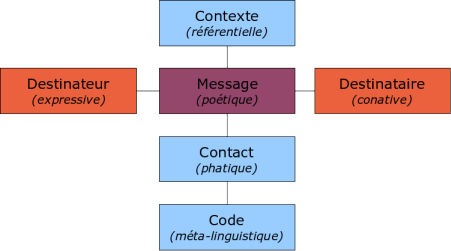
\includegraphics[width=4.6894in,height=2.6114in]{figures/chap3/chapitre3-img5.png}

    \centering[Modèle de Jakobson]{ Modèle de Jakobson, int\'eressante que nous pouvons chercher \`a adapter dans le contexte des \'echanges en ligne.}

\end{figure}

Ainsi, en nous basant sur les mod\`eles des th\'eories de la
communication, nous pouvons peut-\^etre am\'eliorer les mod\`eles
m\'ethodologiques d{\textquoteright}analyse. Nous proposons ici la
notion de \textit{topogramme }comme mod\`ele pour comprendre les motifs
de diffusion des m\`emes, consid\'er\'es comme \textit{topos} ou
\textit{lieux communs. }Le topogramme, en tant que repr\'esentation
graphique des diff\'erentes dimensions et dynamiques lisibles dans les
donn\'ees nous permet donc d{\textquoteright}approcher un travail
\ d{\textquoteright}observation pr\'ecise de la diffusion des m\`emes,
voire par la suite de classification des actes de communication en
ligne. Afin de prendre en compte, les diff\'erents aspects de la
communication, il nous faut donc effectuer une analyse \`a plusieurs
niveaux (multi-layers), regroupant un ensemble de r\'eseaux \`a la fois
s\'emantique, conversationnel et g\'eographique. 



\section{Design de la recherche : M\'ethodologie choisie et schemes d{\textquoteright}analyse retenus}

\subsection[Constitution et collection d{\textquoteright}un corpus de donn\'ees]{Constitution et collection d{\textquoteright}un corpus de donn\'ees}
Afin de poursuivre notre \'etude, nous allons donc proc\'eder \`a
l{\textquoteright}analyse de donn\'ees issues de services de r\'eseaux
sociaux en ligne. La plupart des services de r\'eseaux sociaux en ligne
offrent un large acc\`es car il s{\textquoteright}agit souvent de la
fondation de leurs mod\`eles d{\textquoteright}affaires bas\'es sur la
valorisation et la revente de ces donn\'ees pour le marketing cibl\'e
\citep{Ko2010}. Pour entrer en contact avec la base de donn\'ees, les SNS
mettent \`a disposition une API (\textit{Application Programming
Interface}) qui permet \`a un programme ou une autre application web de
se connecter au service pour demander et obtenir des donn\'ees.
L{\textquoteright}API est donc la premi\`ere source
d{\textquoteright}obtention de donn\'ees depuis les SNS. N\'eanmoins,
les donn\'ees des r\'eseaux sociaux sont soumises \`a
d{\textquoteright}importants enjeux et contraintes tant commerciales,
\'ethiques que politiques dans le cas de la Chine notamment. Les
conditions d{\textquoteright}utilisations techniques et l\'egales
(\textit{Terms of Uses) }de ces donn\'ees sont \'egalement soumises \`a
des changements fr\'equents, \'etroitement li\'es \`a
l{\textquoteright}\'evolution commerciale et technologique de
compagnies souvent tr\`es jeunes. Voici une liste des limitations et
\'ecueils pouvant \^etre rencontr\'es lors de
l{\textquoteright}extraction et de l{\textquoteright}analyse de
donn\'ees des SNS :
ii
\begin{itemize}
\item \textit{Compatibilit\'e }: Une solution technologique devient
facilement caduque lors de l{\textquoteright}\'evolution
d{\textquoteright}une API (ex. Twitter APi v1.0
n{\textquoteright}existe plus, ainsi le code doit \^etre r\'e\'ecrit
pour la version 1.1). 
\item \textit{Disponibilit\'e des donn\'ees :} Chaque API r\'epond \`a
des formats et crit\`eres pr\'ecis et poss\`ede ses propres
limitations. Pour acc\'eder \`a l{\textquoteright}API du moteur de
recherche de Sina Weibo, il faut s{\textquoteright}identifier aupr\`es
de la compagnie gr\^ace \`a une carte d{\textquoteright}identit\'e et
des paiements par requ\^ete sont exig\'es. 
\item \textit{Limitations d{\textquoteright}usage : }Afin de limiter le
trafic et conserver le contr\^ole sur les donn\'ees distribu\'ees, les
SNS mettent en place des limitations d{\textquoteright}acc\`es \`a
leurs serveurs, notamment : limitation du nombre de requ\^etes par
heure, limitation du nombre de requ\^etes par machine (bas\'ee sur
l{\textquoteright}addresse IP), limitation du nombre
d{\textquoteright}utilisateurs connect\'es. Ainsi, Twitter limite \`a
150 requ\^etes API par heure pour un compte non identifi\'e, pouvant
augmenter jusqu{\textquoteright}\`a 500 apr\`es authentification. Les
donn\'ees datant de plus de 7 jours sont payantes, refl\'etant la
valeur d{\textquoteright}un acc\`es en
{\textquotedblleft}temps-r\'eel{\textquotedblright} aux donn\'ees.
\item \textit{L\'egalit\'e }: Les donn\'ees sont soumises aux conditions
de propri\'et\'e d\'ecrites l\'egalement par la firme qui les publient
\citep{Clifton2006}. Ces conditions sont susceptibles de changer. Ainsi,
Twitter a exig\'e en 2012 le retrait a posteriori de nombreux jeux de
donn\'ees publi\'es par des chercheurs depuis plusieurs ann\'ees
parfois \citep{McCreadie2012}. Actuellement, Twitter pr\'ecise notamment
dans ses \textit{Terms of Use: {\textquotedblleft}You may not
resyndicate or share Twitter content, including datasets of Tweet text
and follow relationships{\textquotedblright} }\footnote{ Terms of use
de Twitter, \url{https://dev.twitter.com/terms/api-terms}, consult\'e
le 12 Mars 2013 \`a 17h08}\textit{. ~}
\item \textit{Ethique : }Vous pouvez extraire depuis une API des profils
d{\textquoteright}utilisateurs contenant les informations
qu{\textquoteright}ils ont auparavant publi\'e en ligne (Felt \& Evans,
2008). En exposant les donn\'ees personnelles des utilisateurs, le
chercheur est responsable de l{\textquoteright}usage
qu{\textquoteright}il fait des donn\'ees \citep{Rieder2005} 
\end{itemize}
Afin d{\textquoteright}obtenir des donn\'ees et de contourner les
limitations de l{\textquoteright}API, la pratique dite du
\textit{{\textquotedblleft}scraping{\textquotedblright} }permet
d{\textquoteright}obtenir des donn\'ees \`a l{\textquoteright}aide
d{\textquoteright}un robot qui lit et sauvegarde des parties ou
l{\textquoteright}int\'egralit\'e de pages web. Les moteurs de
recherche utilisent notamment cette technique pour
l{\textquoteright}indexation des pages. Ce type de pratiques est
\'egalement soumis \`a des limitations par les services web (blocage de
l{\textquoteright}IP source) et se situe \`a la limite de la
l\'egalit\'e,voire est explicitement interdite dans le cas de certains
SNS \citep{Petschulat2010}.

Un programme appel\'e \textit{spider }ou \textit{crawler} est charg\'e
d{\textquoteright}effectuer des requ\^etes r\'eguli\`eres \`a
l{\textquoteright}API afin d{\textquoteright}obtenir et collecter les
informations obtenues dans une base de donn\'ees. Plusieurs approches
existent dans les techniques \'echantillonnage de r\'eseau social. La
premi\`ere, fond\'ee sur des mots-cl\'es extraits les posts contenant
des mots ou des hashtags particuliers. La seconde utilise
l{\textquoteright}\'echantillonnage de graphe, collectant au fil des
liens les conversations ou profils des utilisateurs. Classique des
\'etudes statistiques, cet \'echantillonage dit \textit{boule de neige
{\textquotedblleft}\'elargit l{\textquoteright}\'echantillon en partant
d{\textquoteright}un node original pour s{\textquoteright}\'eloigner
vers ses voisins{\textquotedblright}} \citep{Rothenberg1995}. Ici, deux
grandes cat\'egories s{\textquoteright}opposent : les techniques
traversales o\`u les nodes sont classifi\'es apr\`es avoir \'et\'e
visit\'es et les {\textquotedblleft}walk{\textquotedblright}
al\'eatoires o\`u l{\textquoteright}extension du graphe visit\'e se
fait de mani\`ere al\'eatoire \citep{Gjoka2011}. 

Au cours du travail pr\'eparatoire de cette recherche, nous avons tout
d{\textquoteright}abord exp\'eriment\'e plusieurs algorithmes et outils
de collection de donn\'ees afin d{\textquoteright}en comparer les
r\'esultats. Une premi\`ere approche d{\textquoteright}extraction par
utilisateurs a \'et\'e infructueuse car la s\'election du groupe source
(\textit{seeds}) ne permettait pas d{\textquoteright}obtenir des
r\'esultats coh\'erents\footnote{ Code disponible :
\url{https://github.com/sharismlab/Pyweibo}, consult\'e le 14 Mars \`a
5h32}. Par la suite, une autre approche de collecte de donn\'ees via le
d\'eveloppement d{\textquoteright}un plug-in pour le navigateur Google
Chrome\footnote{ Code disponible :
\url{https://github.com/sharismlab/battlefield}, consult\'e le 14 Mars
\`a 5h12\par } nous a permis de tester et d{\textquoteright}apercevoir
les limites de la collection de donn\'ees par mots-cl\'es. Cette
\'etape nous a \'egalement montr\'e l{\textquoteright}int\'er\^et que
peut pr\'esenter une approche collaborative de la collection de
donn\'ees ou de seeds par un syst\`eme de
{\textquotedblleft}curation{\textquotedblright} collaboratifs afin
d{\textquoteright}obtenir des \'el\'ements pr\'ecis de contenus et de
r\'eduire la masse de donn\'ees inutiles qui pollue souvent les jeux de
donn\'ees \citep{Ding2013}. Apr\`es de multiples tests et
comparaisons d{\textquoteright}outils et de librairies, plusieurs
difficult\'es majeures limitaient l{\textquoteright}obtention
d{\textquoteright}une quantit\'e de donn\'ees suffisantes, notamment la
n\'ecessit\'e de ressources assez importantes (en terme de
d\'eveloppement et de disponibilit\'e des machines), un temps
d{\textquoteright}acquisition parfois tr\`es long et
l{\textquoteright}exigence d{\textquoteright}une veille constante sur
les SNS pour identifier un m\`eme au bon moment (les tweets de Sina
Weibo devenant indisponibles via l{\textquoteright}API au-del\`a de 7
jours). La premi\`ere limite se situe bien s\^ur dans la capacit\'e
d{\textquoteright}une personne seule \`a mener \`a bien cette large
t\^ache. Nous avons donc choisi de consid\'erer les jeux de donn\'ees
collect\'es sur Sina Weibo disponibles sur l{\textquoteright}Internet.
Une fois \'ecart\'es les nombreux jeux tronqu\'es, modifi\'es ou
incomplets, nous avons pu obtenir plusieurs jeux de donn\'ees provenant
de recherches pr\'ealables dans le domaine particulier de
l{\textquoteright}\'echantillonnage \citep{Ding2013} ou ayant servi
de bases \`a des \'etudes pr\'ec\'edentes \citep{Gao2012, Leiden2010}. Finalement, nous avons identifi\'e le jeu de donn\'ees
constitu\'e lors du projet \textit{Weiboscope }de
l{\textquoteright}Universit\'e de Hong Kong comme r\'epondant \`a nos
besoins en termes de dimensions (temps, nombre
d{\textquoteright}utilisateurs observ\'es), taille (nombre de tweets)
et contenus (g\'eo-localisation, pr\'esence des tweets censur\'es).



Notre travail d{\textquoteright}analyse s{\textquoteright}appuie donc
sur ce jeu de donn\'ees collect\'e sur le service de microblog Sina
Weibo par le \textit{Journalism and Media Studies Centre} (JMSC) de
l{\textquoteright}Universit\'e de Hong Kong lors de son projet
\textit{Weiboscope}. T\'el\'echargeable ouvertement, la publication de
ce jeu de donn\'ees a pour objectif de
\textit{{\textquotedblleft}enables academic use of the data for better
understanding of the social }\textit{media in China and making the
Chinese media system more transparent.{\textquotedblright}}\footnote{
Le jeu de donn\'ees Weiboscope est disponible \`a l{\textquoteright}adresse :
\url{http://147.8.142.179/datazip/}, consult\'e le 14 Mars \`a 17h21 }\textit{ }Il s{\textquoteright}agit
d{\textquoteright}un \'echantillonnage al\'eatoire de messages
\textit{(random sampling)} effectu\'e quotidiennement durant toute
l{\textquoteright}ann\'ee 2012 sur un panel d{\textquoteright}environ
350 000 utilisateurs ayant au moins 1000 followers \citep{Fu2013}. La totalit\'e du jeu de donn\'ees comprend 226,841,122 messages
r\'epartis sur 52 semaines, dont des messages ayant \'et\'e supprim\'es
par les utilisateurs eux-m\^emes ou par les administrateurs de Sina
Weibo eux-m\^emes - parfois sur ordre du gouvernement chinois
(\textit{ibid}, 2013).

\begin{figure}
    \centering
    \begin{tabular}{c|c}
        mid  &
        Unique pseudo message ID\\
        retweeted\_status\_mid  &
        Pseudo message ID of the original message (Only available if the row of
        interest is a retweet)\\
        Uid &
        Pseudo user ID\\
        retweeted\_uid &
        Pseudo user ID of the original poster (Only available if the row of
        interest is a retweet)\\
        Source &
        The application name of the client program\\
        Image &
        With image? (1= Yes, 0=No)\\
        text  &
        body of the message. Any address handle (@xxxx:) is replaced by either
        the pseudo user ID or ukn (uknown)\\
        geo &
        GIS information. Please refer to the Sina Weibo API documentation:
        \url{http://goo.gl/Um8SS}\\
        created\_at &
        Original posting time\\
        deleted\_last\_seen &
        The last seen time before this message was missing from the user
        timeline\\
        permission\_denied  &
        {\textquotesingle}permission denied{\textquotesingle} status is marked
        when the message was found missing in the timeline and the API return
        message was {\textquotesingle}permission denied{\textquotesingle} - See
        details in (Fu, Chan, Chau 2013)\\
    \end{tabular}
 \end{figure}





Ce jeu de donn\'ees a \'et\'e mis \`a disposition sous une forme
anonymis\'ee o\`u les identifiants des messages et des utilisateurs ont
\'et\'e remplac\'es par des pseudo-identifiants. La collection des
donn\'ees a \'et\'e effectu\'ee sur une s\'erie
d{\textquoteright}utilisateurs (g\'en\'eration al\'eatoire
d{\textquoteright}identifiants dont l{\textquoteright}existence est
ensuite valid\'ee) pour donner \textit{{\textquotedblleft}une image
repr\'esentative des usages et utilisateurs de Sina Weibo (...) dont
les \'etudes auparavant limit\'ee \`a des analyses non-al\'eatoire
(...) se cantonnaient aux utilisateurs les plus
populaires{\textquotedblright} }\citep{Fu2013}. Ainsi, plut\^ot que
de consid\'erer uniquement les
{\textquotedblleft}stars{\textquotedblright} de Sina Weibo, cet
\'echantillon s{\textquoteright}attache \`a refl\'eter \'egalement les
pratiques des utilisateurs
{\textquotedblleft}lambda{\textquotedblright}. Ce jeu de donn\'ees a
d\'ej\`a \'et\'e partiellement \'etudi\'e dans le but de comprendre la
d\'emographie des utilisateurs de Sina Weibo, leurs activit\'es et les
comportements pouvant permettre de pr\'edire les r\'eactions notamment
de censure \citep{Fu2013}. La d\'emographie des utilisateurs se
composent de 55\% d{\textquoteright}hommes habitant principalement dans
les grandes villes de Chine (P\'ekin, Canton, Shanghai). Une des
d\'ecouvertes importantes est le tr\`es faible taux de cr\'eation
originale de messages malgr\'e une activit\'e importante des
utilisateurs, indiquant que l{\textquoteright}essentiel de
l{\textquoteright}activit\'e sur Sina Weibo se constitue de re-posts et
de commentaires. Le jeu de donn\'ees est accompagn\'e des informations
succintes de profil des utilisateurs dont le lieu, rempli par eux, sans
n\'eanmoins fournir leurs noms d{\textquoteright}utilisateur
v\'eritables. Notre travail de recherche s{\textquoteright}articule
autour d{\textquoteright}une nouvelle lecture de ce jeu de donn\'ees
unique.

\subsection[Identification des m\`emes en tant que {\textquotedblleft}clusters{\textquotedblright}]{Identification des m\`emes en tant que {\textquotedblleft}clusters{\textquotedblright}}
Une fois l{\textquoteright}acquisition des donn\'ees effectu\'ees, il
s{\textquoteright}agit d\'esormais de savoir les analyser correctement
pour y d\'eceler les m\`emes que nous souhaitons consid\'erer. Les
travaux dans le domaine de la d\'etection et
l{\textquoteright}identification de m\`emes dans les donn\'ees de
r\'eseaux sociaux restent encore peu nombreux. Une des \'etudes
pionni\`eres est l{\textquoteright}outil \textit{MemeTracker }(devenu
\textit{NIFTY}) con\c{c}u en 2009 par le \textit{SNA Project }de
l{\textquoteright}Universit\'e de Stanford \citep{Leskovec2009}. Cet
outil permet une \'etude sous forme de graphes de la diffusion de
phrases dans un vaste corpus de texte mais n{\textquoteright}est pas
adapt\'e \`a la langue chinoise. La discussion sur la mod\'elisation
math\'ematiques des m\`emes \citep{Ahmad2006, Nye2011} \'emane souvent
de recherches en informatique cherchant \`a prendre en consid\'eration
diff\'erents facteurs de diffusion lors de l{\textquoteright}analyse
machine de donn\'ees \citep{Zubiaga2011, Wang2011)},
consid\'erant le m\`eme comme un vecteur de modification du r\'eseau
lui-m\^eme \citep{Ienco2010}. Plus marginal, des \'etudes
s{\textquoteright}int\'eressent aux dynamiques g\'eographiques des
m\`emes \citep{Kamath2013}. N\'eanmoins, aucune de ces diff\'erentes
approches ne permet d{\textquoteright}apporter une r\'eponse
technologique ou algorithmique satisfaisante pour
l{\textquoteright}identification de m\`emes Internet dans un ensemble
de donn\'ees issu des r\'eseaux sociaux. Afin de d\'eceler les m\`emes
dans un vaste ensemble textuel, nous devons y d\'eceler des motifs de
diffusion particuliers. La d\'enomination \textit{machine learning
}regroupe un ensemble d{\textquoteright}algorithmes qui permettent
d{\textquoteright}explorer des jeux de donn\'ees pour en extraire des
repr\'esentations et y identifier des propri\'et\'es
(\textit{features}) particuli\`eres. Bas\'e sur les sciences
statistiques, ces algorithmes font usage de mesures de similarit\'e
pour classifier les \'el\'ements d{\textquoteright}un corpus. Les
cat\'egories utilis\'ees pour la classification peuvent \^etre
d\'efinies au pr\'ealable par l{\textquoteright}utilisateur -
c{\textquoteright}est le \textit{{\textquotedblleft}supervised
learning{\textquotedblright} }ou inf\'er\'ees du jeu de donn\'ees
lui-m\^eme dans le cas du \textit{{\textquotedblleft}unsupervised
learning{\textquotedblright}} pour la d\'etection de \textit{clusters
}\citep{Breiman2001}\textit{. }La multitude d{\textquoteright}algorithmes
de \textit{machine learning }disponibles pour la d\'etection de
clusters au sein d{\textquoteright}un corpus textuel ou
d{\textquoteright}un r\'eseau social \citep{Nettleton2013, Robbins2013}
rend l{\textquoteright}identification d{\textquoteright}une solution
difficile. De plus, les algorithmes utilis\'es traditionnellement pour
l{\textquoteright}analyse de documents textuels (\textit{topic
modeling, LSA}) se heurtent au caract\`ere tr\`es disparate des corpus
issus des r\'eseaux sociaux (\textit{text sparsity issue) }faisant
diminuer drastiquement leur efficacit\'e \citep{Hong2010}. 



Ferrara \& al. \citep{Ferrara2013} propose dans un papier intitul\'e
{\textquotedblleft}\textit{Meme clustering in social
media}{\textquotedblright} un algorithme utilisant la classification
automatique non-supervis\'ee pour d\'etecter des m\`emes dans un corpus
de donn\'ees de r\'eseaux sociaux. Ce travail r\'ecent propose de tenir
compte non seulement des textes et hashtags, mais aussi des liens et
des mod\`eles de diffusion pour identifier des groupes de messages
int\'eressants et proc\'eder au \textit{clustering }des m\`emes.
L{\textquoteright}algorithme s{\textquoteright}articule autour du
concept de {\textquotedblleft}protom\`emes{\textquotedblright},
repr\'esentant les \'el\'ements fondamentaux d{\textquoteright}un
m\`eme en cours de cr\'eation \citep{Gabora1997}. Dans le contexte des
m\'edias sociaux, le protom\`eme est d\'efini par les entit\'es (liens,
hashtags...), mots-cl\'es et s\'equences de conversation qui constitue
le m\`eme en devenir. En identifiant puis comparant les diff\'erents
protom\`emes pr\'esents dans chaque tweet, il est possible
d{\textquoteright}y d\'etecter des similarit\'es et de deviner les
m\`emes en formation. 

\begin{figure} 
    \centering

    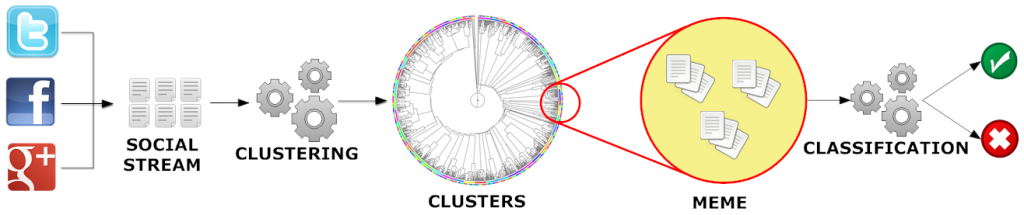
\includegraphics[width=5.8894in,height=1.2114in]{figures/chap3/chapitre3-img6.png}
    \caption{Algorithme de reconnaissance de mème (clustering) \citep{Ferrara2013}}
\end{figure}

Cet algorithme suppose donc d{\textquoteright}extraire dans un premier
temps les \'el\'ements remarquables du corpus de tweets afin
d{\textquoteright}\'etablir des repr\'esentations de ces protom\`emes
contenant les \'el\'ements \`a comparer : \textit{phrases} (texte
brut), \textit{mentions }(@, RT), \textit{hashtags }et \textit{urls}.
Pour constituer ces jeux de protom\`emes, nous utilisons le pattern
\textit{map-reduce} qui permet de chercher et lister des \'el\'ements
dans un vaste jeu de donn\'ees \textit{(map)} avant de les regrouper
dans une liste \textit{(reduce)}. Une fois ces protom\`emes
constitu\'es nous proc\'edons \`a leurs comparaisons selon plusieurs
crit\`eres :
v
\begin{itemize}
\item \textit{Similarit\'e de texte }: comparant le contenu texuel de
chaque protom\`eme 
\item \textit{Similarit\'e d{\textquoteright}utilisateurs} : comparant
les utilisateurs contenus dans chaque protom\`eme
\item \textit{Similarit\'es de tweet }: recherchant les tweets
identiques dans diff\'erents protom\`emes
\item \textit{Similarit\'e de diffusion : }consid\'erant les
r\'ef\'erences aux utilisateurs contenus dans chaque protom\`eme
\end{itemize}
Ici nous utilisons la \textit{s\'emantique vectorielle} (Support Vector
Machine) afin de comparer les \'el\'ements des protom\`emes gr\^ace \`a
une repr\'esentation alg\'ebrique sous formes de vecteurs. Pratique
ancienne de l{\textquoteright}alg\`ebre lin\'eaire appliqu\'ee \`a la
science informatique \citep{Salton1975}, il s{\textquoteright}agit de
permettre la conversion d{\textquoteright}objets textuels (mots,
identifiants, images...) sous une forme ais\'ement comparable. Pour
convertir le texte sous forme vectorielle, l{\textquoteright}algorithme
classique Tf-idf (\textit{Term Frequency - Inverse Document Frequency})
est utilis\'e \citep{Soucy2005}. Les autres mesures de similarit\'e sont la
\textit{mesure cosine (}ou \textit{similarit\'e cosinus) }des
protom\`emes convertis sous forme de vecteurs binaires. Une fois ces
diff\'erentes valeurs de similarit\'e calcul\'ees, nous utilisons les
scalaires d\'efinis dans le papier de r\'ef\'erence pour assigner des
poids \`a chacun des vecteurs et les combiner en une seule valeur
\citep{Ferrara2013}. Cette matrice de valeurs de similarit\'e nous permet
alors de d\'efinir les protom\`emes les plus similaires et
d{\textquoteright}identifier ainsi des \textit{clusters }dans les
donn\'ees correspondant aux m\`emes.



Si cette approche offre des r\'esultats probants sur de petits volumes
(quelques centaines de tweets), la tr\`es grande demande en puissance
de calcul et ressources m\'emoires n\'ecessaires rendent le traitement
d{\textquoteright}un jeu donn\'ees plus vaste irr\'ealisable. Les
op\'erations de comparaison et le calcul de similarit\'es sur de vastes
volumes de donn\'ees font cro\^itre tr\`es rapidement la complexit\'e
des algorithmes et ainsi la quantit\'e de calculs \`a effectuer. Le
calcul du co\^ut d{\textquoteright}un algorithme se fait au travers des
notions dites de domination, avec notamment le {\textquotedblleft}grand
O{\textquotedblright} exprim\'e \textit{O(f(n)) }qui fait correspondre
\`a la complexit\'e d{\textquoteright}un algorithme une fonction
\textit{f} de la quantit\'e d{\textquoteright}information manipul\'ee
\textit{n. }Ainsi pour un algorithme courant de complexit\'e
\textit{O(n}\textit{\textsuperscript{2}}\textit{), }les ressources de
calcul \textit{(computation)} et de m\'emoire (RAM ou stockage)
n\'ecessaires augmentent de mani\`ere exponentielle \`a chaque
\'el\'ement ajout\'e au corpus \textit{n}. L{\textquoteright}algorithme
de {\textquotedblleft}meme clustering{\textquotedblright} d\'ecrit par
Ferrara atteint donc un co\^ut exorbitant devant un large volume de
donn\'ees comme celui du jeu Weibosope. La limite physique de calcul
est rapidement atteinte rendant impossible le franchissement du pallier
exp\'erimental et la v\'erification des hypoth\`eses de travail \`a une
\'echelle suffisante.

\subsection[ L{\textquoteright}identification des m\`emes par hashtags ]{L{\textquoteright}identification des m\`emes par hashtags }
Les travaux en sciences humaines sur les m\`emes \citep{Bauckhage2011,
Coscia2013, Knobel2007} et les sites sp\'ecialis\'es \citep{Buchel2012, Bernstein2011} pr\'esente bien souvent un m\`eme sous la forme
d{\textquoteright}un titre (mot ou groupe de mots) accompagn\'e
d{\textquoteright}une collection d{\textquoteright}images ou/et de
vid\'eos, ainsi qu{\textquoteright}un texte explicatif (mise en
contexte) et des indications sur les dates de parution et son
\'evolution dans le temps. Ici, un ou des auteurs se saisissent des
mat\'eriaux bruts du web et les rassemblent pour reconstituer une
vision particuli\`ere du m\`eme, aussi repr\'esentative que possible.
Cette approche n\'ecessite peu de d\'eploiement technologique (un
copier/coller suffit souvent), mais exige n\'eanmoins une forte
connaissance et un suivi r\'egulier du terrain Internet pour y
d\'enicher ces repr\'esentations du m\`emes. Cette d\'emarche que nous
nommerons \textit{ethnographique }s{\textquoteright}apparente \`a de la
curation de contenu \citep{Buckingham2006}. Les \textit{hashtags }(en
fran\c{c}ais {\textquotedblleft}mots-di\`eses{\textquotedblright}) sont
utilis\'es dans l{\textquoteright}\'ecriture sur les r\'eseaux sociaux
et se pr\'esentant dans Sina Weibo sous la forme d{\textquoteright}un
mot entour\'e de deux di\`eses - ex. \textit{\#mot-cl\'e\#}. Marqueur
particulier, le hashtag permet \`a un interlocuteur de proc\'eder \`a
une d\'enotation ou connotation du message original \citep{Romero2011} ou
d{\textquoteright}affirmer son caract\`ere \'ev\`enementiel (lors
d{\textquoteright}un \'ev\`enement sportif, d{\textquoteright}une
conf\'erence, etc). Facile \`a identifier dans la masse des donn\'ees
en ligne, il permet de d\'esigner un ensemble de contenus sous un
m\^eme signe. Ainsi, il est un vecteur important permettant de
collecter simplement une large masse d{\textquoteright}informations
autour d{\textquoteright}un m\`eme. La constitution
d{\textquoteright}un corpus autour d{\textquoteright}un
{\textquotedblleft}hashtag{\textquotedblright} pr\'esente n\'eanmoins
plusieurs limites. Premi\`erement, le m\`eme est par d\'efinition un
objet en mutation. Ainsi, il est souvent difficile de
l{\textquoteright}identifier une bonne fois pour toute par un ou
plusieurs de mot-cl\'es. De plus, le m\`eme existe bien souvent sous la
forme d{\textquoteright}images ou de vid\'eos qui ne sont pas
n\'ecessairement l\'egend\'ees ou r\'ef\'erenc\'ees et donc peu
accessible \`a une recherche {\textquotedblleft}plein
texte{\textquotedblright}. Ainsi, une approche pour la recherche de
m\`emes ne peut \^etre enti\`erement textuelle et doit
s{\textquoteright}int\'eresser aux autres forme de contenus web
(notamment les liens et les hashtags). De plus, l{\textquoteright}ajout
de hashtags dans les messages est un acte volontaire non
syst\'ematique. Ainsi, si l{\textquoteright}identification de certains
m\`emes peut se faire gr\^ace \`a la recherche de hashtags,
l{\textquoteright}ensemble des messages contenant des hashtags ne
recouvrent pas syst\'ematiquement un m\`eme. Comme nous le verrons, les
hashtags sont bien souvent de simples artefacts de campagne marketing
en ligne.



Afin de proc\'eder \`a l{\textquoteright}analyse des m\`emes, nous avons
donc index\'e l{\textquoteright}ensemble des contenus du corpus
Weiboscope contenant des hashtags sur toute l{\textquoteright}ann\'ee
2012 (30 millions sur un total de 200 millions tweets environs). Nous
avons donc dans un premier temps extrait l{\textquoteright}ensemble des
messages contenant un ou des hashtags de l{\textquoteright}ensemble des
donn\'ees avant de les classifier pour obtenir des jeux de donn\'ees
coh\'erents par hashtags. Une premi\`ere contrainte ici est propre au
traitement informatique de la langue chinoise qui constitue le langage
majoritaire de notre corpus. L{\textquoteright}absence
d{\textquoteright}espace entre les diff\'erents caract\`eres de la
phrase en chinois oblige \`a prendre en compte la s\'emantique de la
phrase pour proc\'eder \`a sa segmentation. Cette question usuelle pour
les usagers du NLP (\textit{Natural Language Processing}) en chinois
est un sujet de recherche encore tr\`es discut\'e \citep{Qiu2013}.
L{\textquoteright}identification de la meilleure option parmi la
multitude des librairies et logiciels disponibles pour la segmentation
puis le NLP en chinois a \'et\'e un aspect pr\'eliminaire importants de
notre travail d{\textquoteright}analyse de donn\'ees. Nous avons ainsi
r\'ealis\'e de nombreux benchmark afin de comparer les diff\'erentes
technologies existantes. Un travail men\'e avec
l{\textquoteright}\'equipe du site Internet
d{\textquoteright}actualit\'e scientifique \textit{Guokr }\`a P\'ekin
nous a amen\'e \`a choisir en premier lieu un algorithme de
segmentation d\'evelopp\'e sur la base de textes en chinois
ancien\footnote{ gkSeg : \textit{{\textquotedblleft}Yet another Chinese
word segmentation package based on character-based tagging heuristics
and CRF algorithm{\textquotedblright}
}\url{https://github.com/guokr/gkseg}, consult\'e le 14 Mars \`a
18:28}. Apr\`es plusieurs tentatives, nous avons pr\'ef\'er\'e le
segmenteur open-source Jieba\footnote{
\url{https://github.com/fxsjy/jieba}, consult\'e le 14 Mars \`a 18:30}
plus g\'en\'ereux en termes de fonctionnalit\'es et permettant de
meilleures performances. Une fois la phrase chinoise segment\'ee, la
seconde \'etape consiste \`a supprimer tous les mots les plus communs
\textit{(stopwords)}, ainsi que la ponctuation et
d{\textquoteright}autres caract\`eres trop courants afin de pr\'eserver
uniquement les mots riches de sens dans les phrases (les mots-cl\'es).
L{\textquoteright}extraction des hashtags est effectu\'ee gr\^ace \`a
une expression r\'eguli\`ere qui scanne le texte pour identifier et
pr\'eserver uniquement les caract\`eres situ\'es entre les deux signes
di\`ese (\#). Sur un total d{\textquoteright}environ 30 millions de
tweets contenant des hashtags, nous avons choisi de retenir seulement
les hashtags poss\'edant plus de 1000 messages. Nous avons ensuite
d\'ecid\'e d{\textquoteright}ignorer les 1000 hashtags les plus
utilis\'es car ils ne pr\'esentaient pas d{\textquoteright}int\'er\^et
pour notre \'etude, \'etant la plupart du temps des noms de marque ou
des mots-cl\'es trop g\'en\'eraux (par exemple :
{\textquotedblleft}bonne nuit{\textquotedblright},
{\textquotedblleft}nouvelles de sports{\textquotedblright},
{\textquotedblleft}photos de nourriture{\textquotedblright}, etc.) 


\begin{figure}
    \centering
    
    \subfloat[Hashtags les plus utilis\'es pendant la 1\`ere semaine de 2012] {
        \begin{tabular}{c|c|c|c}
            hashtags & users &  actions & tweets \\
            \zh{吴奇隆} 201 & 13243 & 22349  \\
            \zh{一起到老} 182 & 0 & 364  \\
            \zh{春运} 92 & 13 & 256  \\
            \zh{轻松一刻} 92 & 11 & 240  \\
            \zh{人品值分析} 90 & 490 & 321  \\
            \zh{朝阳区} 88 & 49 & 165  \\
            \zh{理性态小度} 87 & 0 & 329  \\
            \zh{美图GIF} 87 & 101 & 404  \\
            \zh{我正在听} 86 & 6 & 330  \\
            \zh{微盘签到} 84 & 304 & 305  \\
            \zh{2012来了} 83 & 206 & 309  \\
            \zh{中级达人} 83 & 0 & 159  \\
            \zh{分享} 82 & 87 & 563  \\
            \zh{星座} 82 & 5 & 195  \\
            \zh{极速互联随我行} 81 & 317 & 701  \\
            \zh{微信} 80 & 11 & 288  \\
            \zh{微博达人} 80 & 9 & 364  \\
            \zh{2012} 79 & 37 & 270  \\
            \zh{那些年} 79 & 106 & 217  \\
            \zh{晚安心语} 78 & 27 & 150  \\
            \zh{周杰伦} 77 & 130 & 286  \\
            \zh{多多cosplay} 15 & 414 & 463  \\
        \end{tabular}
    }

    \subfloat[Volume de tweets pendant la semaine ]{
        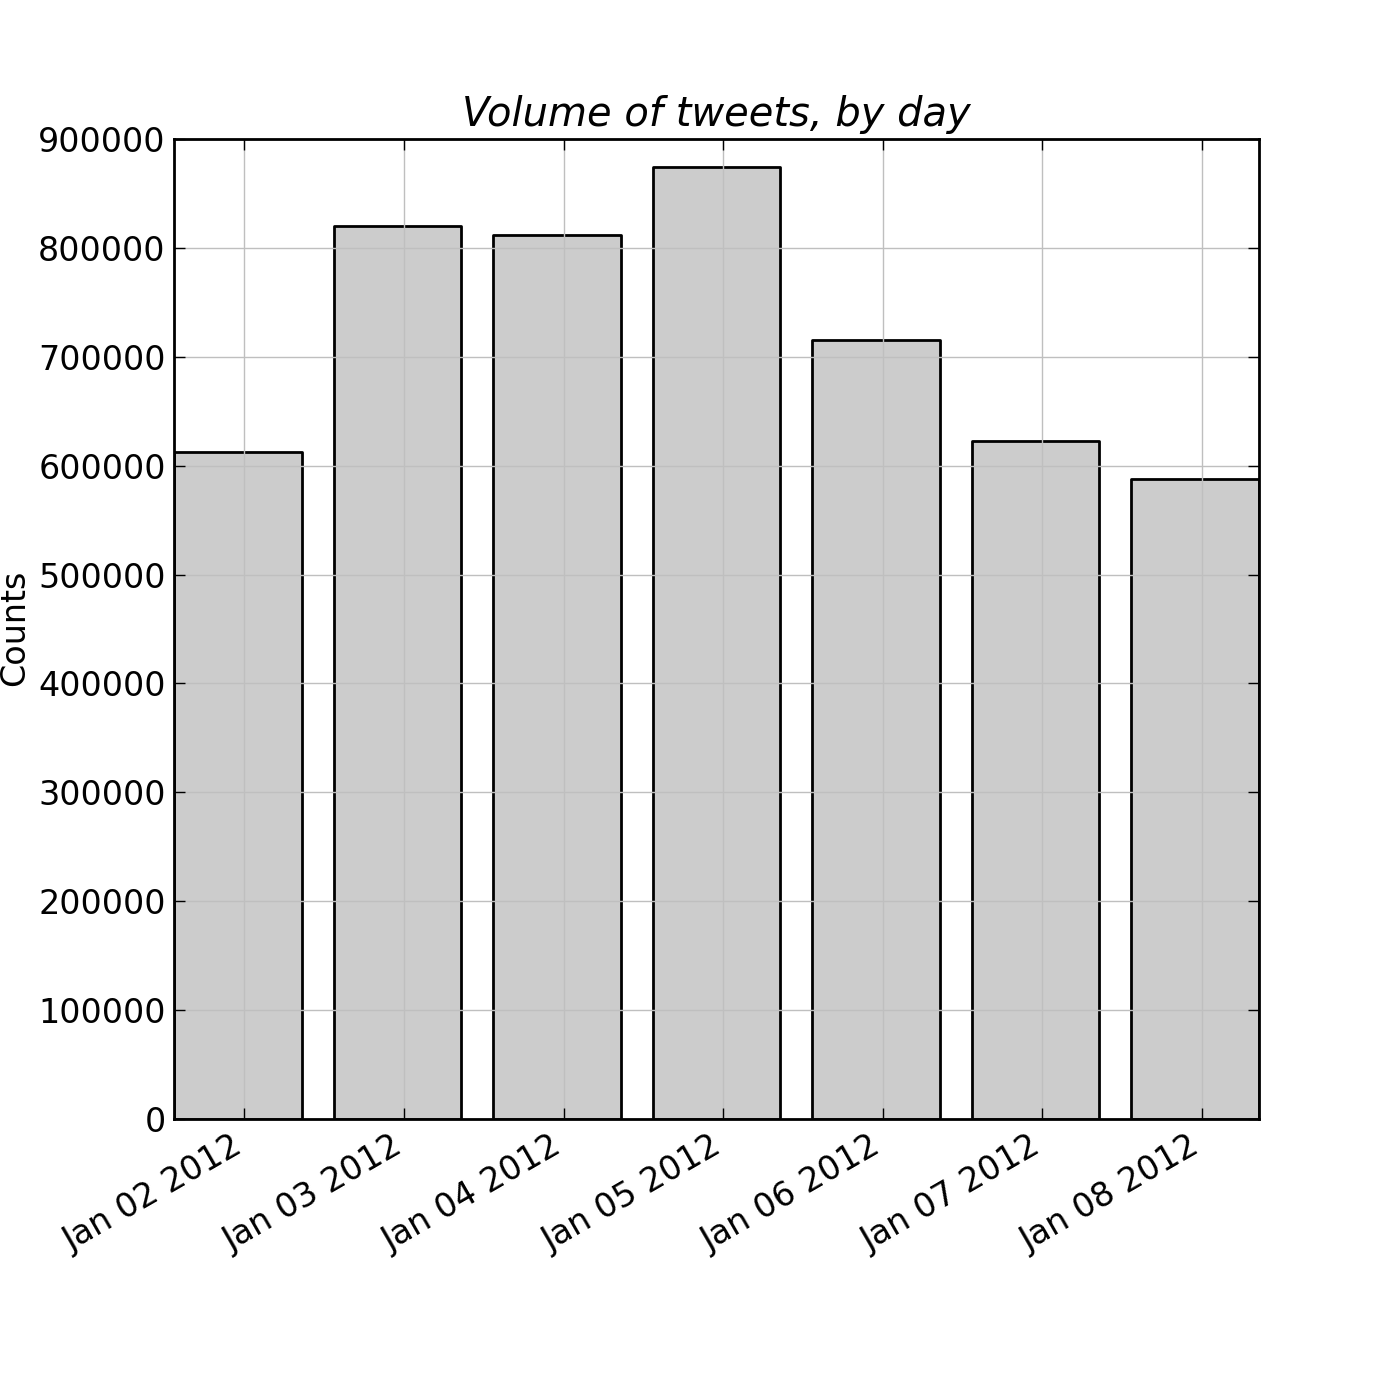
\includegraphics[width=3.2004in,height=3.2004in]{figures/chap3/chapitre3-img7.png}
    }

    \caption[Volume de tweets et hashtags pour la semaine 1]{Les r\'esultats concernant la 1\`ere semaine de l{\textquoteright}ann\'ee 2012 donnent un aper\c{c}u du volume analys\'e : 5,044,331 tweets, 398 392 utilisateurs uniques cit\'es (dans un total de 2 115 544 mentions), 264 651 urls uniques (pour un total de 426 914) et 44 382 hashtags uniques (pour un total de 244285).}
\end{figure}



Notre \'etude vise\`a \'etudier les dynamiques conversationnelles et
nous devons donc d\'eterminer les plus ad\'equats parmi des hashtags de
nature souvent tr\`es diff\'erentes. Pour ce faire, nous avons
s\'electionn\'e pour chaque jeu de donn\'ees (chaque hashtag) deux
mesures significatives : premi\`erement, le volume de messages ;
deuxi\`emement, la quantit\'e d{\textquoteright}\'echanges et
d{\textquoteright}interactions effectives entre les utilisateurs
(commentaires, retweets, etc.). Ces deux mesures nous permettent de
nous assurer que 1) nous poss\'edons une quantit\'e suffisante de
messages pour mener \`a bien l{\textquoteright}\'etude et que 2) la
discussion a bien eu lieu et qu{\textquoteright}il ne
s{\textquoteright}agit pas de messages redondants ou non reli\'es entre
eux. Nous avons choisi d{\textquoteright}ignorer les \'echanges
domin\'es \`a plus de 80\% par le m\^eme utilisateur pour \'eviter la
pollution de l{\textquoteright}\'etude par l{\textquoteright}activit\'e
de robots. Le graphe ci-dessous permet d{\textquoteright}observer la
distribution de 429 hashtags poss\'edant tous plus de 1000 tweets et
1000 \'echanges : l{\textquoteright}axe vertical repr\'esente la
quantit\'e d{\textquoteright}actions (\'echanges) et
l{\textquoteright}axe horizontal le volume des conversations. Tout en
bas du graphe se trouvent donc les hashtags ayant \'et\'e les moins
discut\'es, avec en haut ceux aux conversations les plus intenses. La
taille des points illustre le volume de messages et la couleur la
quantit\'e de %
%je ne comprends pas le code couleur
conversations.

\begin{figure}
    \centering
    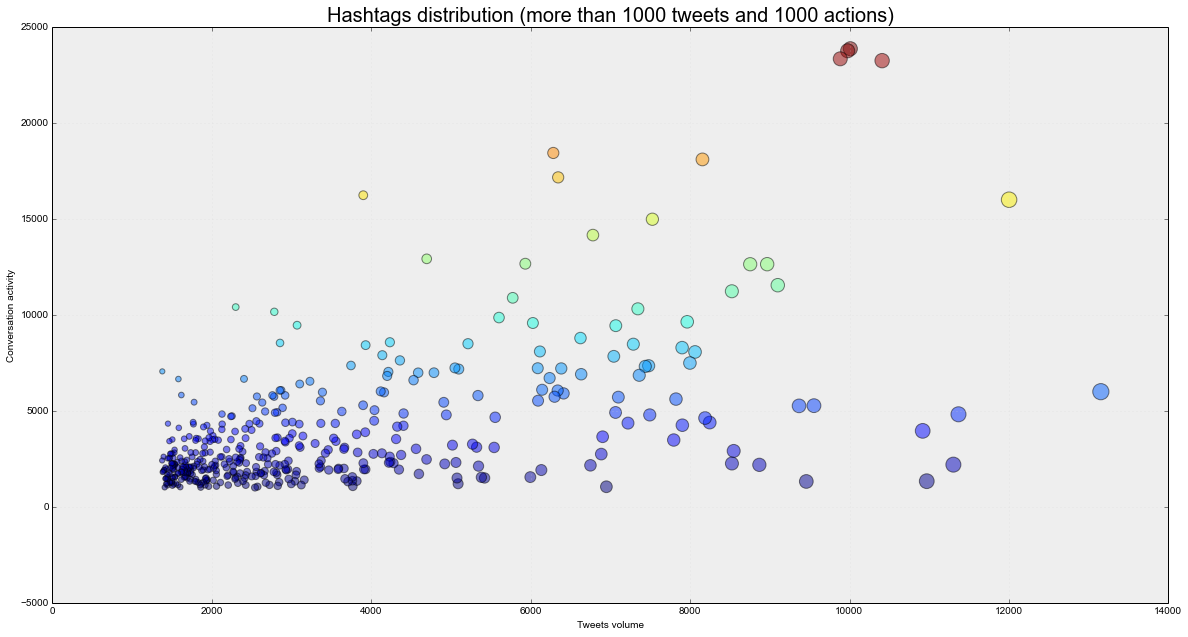
\includegraphics[width=6.0114in,height=3.2114in]{figures/chap3/chapitre3-img8.png}
    \caption{Distribution des 429 hashtags s\'electionn\'es }
\end{figure}


En proc\'edant \`a l{\textquoteright}\'etiquetage des hashtags les plus
actifs durant l{\textquoteright}ann\'ee 2012 sur Sina Weibo (figure 2
ci-dessus), nous constatons que la plupart sont associ\'es \`a des
activit\'es commerciales, de loisirs ou de divertissement. Ici nous
observons que les usages majoritaires du r\'eseau social Sina Weibo
correspondent pour la plupart \`a ceux d{\textquoteright}autres
mass-m\'edias plus traditionnels de par le monde. Le commerce en ligne
occupe notamment une place pro\'eminente. La marque de t\'el\'ephonie
mobile chinoise \textit{Xiaomi }est abondamment cit\'ee, refl\'etant
son importance croissante dans le march\'e chinois et surtout sa
strat\'egie commerciale qui cible abondamment les r\'eseaux sociaux
avec de nombreux hashtags tr\`es discut\'es (notamment
\textit{{\textquotedblleft}Fans de Xiaomi{\textquotedblright}
}[5C0F?][7C73?][7C89?][4E1D?] ). Egalement, de nombreuses campagnes
promotionnelles d{\textquoteright}ouverture ou
d{\textquoteright}anniversaire de magasins ont r\'eussi \`a se hisser
dans le jeu de t\^ete des hashtags les plus discut\'es. Radio-crochets
ou chanteurs reconnus, les stars de la t\'el\'evision et de la chanson
sont aussi pr\'esents dans le peloton de t\^etes des discussions sur
Sina Weibo. Le c\'el\`ebre chanteur Han Geng notamment compte pr\`es
d{\textquoteright}une dizaine de hashtags le concernant parmi les 500
les plus discut\'es (\textit{{\textquotedblleft}Han Geng fait une pub
pour Nokia{\textquotedblright}, {\textquotedblleft}Han Geng va en
Italie{\textquotedblright}, {\textquotedblleft}Han Geng fait une pub
Pepsi{\textquotedblright}, {\textquotedblleft}Han Geng refuse une
interview{\textquotedblright}, etc.)} Ici encore, le r\'eseau social
agit comme le prolongement des mass m\'edia traditionnels,
\'el\'ement-cl\'e des nouvelles strat\'egies de publicit\'es en ligne,
parfois particuli\`erement agressives comme dans le cas de Han Geng.
Les contenus de la t\'el\'evision sont largement relay\'es et
discut\'es, notamment les s\'eries t\'el\'evisuelles. Le cin\'ema est
aussi repr\'esent\'e. Le film comique chinois \textit{Lost in Thailand
}sorti en D\'ecembre 2012 d\'epeint les aventures d{\textquoteright}un
chinois en vacances en Thailande. Premier grand succ\`es commercial du
box-office chinois, sa popularit\'e se refl\`ete dans
l{\textquoteright}importance au sein des discussions en ligne. Les
tendances des ventes du livre sont refl\'et\'ees par de nombreux
best-seller sur {\textquotedblleft}l{\textquoteright}am\'elioration de
soi{\textquotedblright} ou la {\textquotedblleft}r\'eussite
\'economique{\textquotedblright}\textit{. }Ce type de hashtags ne se
limite pas au support web mais s{\textquoteright}origine directement
dans d{\textquoteright}autres m\'edias plus traditionnels. Le
gouvernement lui-m\^eme utilise Sina Weibo pour faire passer ses
messages avec un hashtag \textit{{\textquotedblleft}information
officielle{\textquotedblright} }utilis\'e notamment pour des d\'ementis
publics ou droit de r\'eponse par l{\textquoteright}entreprise Sina,
propri\'etaire du service. \'Egalement outil de conversation, les
discussions sur les r\'eseaux sociaux parlent de la vie de tous les
jours. La situation routi\`ere et les bouchons dans chaque ville sont
un des grands sujets de discussions. Ce sont dans ces \'echanges
quotidiens que se cristallisent plus particuli\`erement les enjeux
politiques et m\'ediatiques des r\'eseaux sociaux. Nouveau caf\'e du
commerce, les commentaires sur les faits divers et
l{\textquoteright}actualit\'e mettent souvent \`a jour les
dysfonctionnements de syst\`emes politiques, urbains ou l\'egaux. Il
est int\'eressant n\'eanmoins de noter que parmi les hashtags les plus
discut\'es, les ph\'enom\`enes de suppression de contenus par les
administrateurs (censure) restent tr\`es marginal. Le \textit{China
Digital Times} de UC Berkeley maintient une liste des mots interdits
sur Sina Weibo depuis plusieurs anne\'es \citep{Ng2013}. En comparant cette
liste de mots censur\'es \`a celle des hashtags, nous avons pu voir
qu{\textquoteright}aucun des 3000 hashtags les plus utilis\'es en 2012
n{\textquoteright}a \'et\'e soumis a une interdiction m\^eme temporaire
sur Sina Weibo. Les hashtags les plus sujets \`a la censure ne sont pas
en lien avec des domaines politiques ou des sujets sensibles, mais
plut\^ot avec des contenus \`a caract\`ere pornographique (la
pornographie est interdite en Chine). Refl\'etant les usages
majoritaires (commerce, loisirs, etc.), les hashtags v\'ehiculent des
contenus souvent moins controvers\'es et les {\textquotedblleft}mots
censur\'es{\textquotedblright} sont plus \`a m\^eme
d{\textquoteright}appara\^itre dans des discussions informelles.

\subsection[Visualisation du graphe conversationnel d{\textquoteright}utilisateurs]{Visualisation du graphe conversationnel d{\textquoteright}utilisateurs}
Apr\`es avoir identifi\'e diff\'erents \textit{m\`emes parmi }les
hashtags les plus discut\'es de l{\textquoteright}ann\'ee 2012, nous
allons maintenant proc\'eder \`a l{\textquoteright}analyse du
d\'eroulement des \'echanges d{\textquoteright}apr\`es chacun des
diff\'erents corpus de donn\'ees. Plusieurs types de graphes peuvent
\^etre extraits :


\begin{itemize}
\item \textbf{Graphe social statique : }repr\'esentant les relations
pr\'e-existantes dans la structure du r\'eseau \'etudi\'e (untel est
ami avec untel, untel suit untel, etc.)
\item \textbf{Graphe conversationnel~}: repr\'esentant toutes les
interactions qui entourent et structurent la diffusion de messages 
\item \textbf{Graphe de diffusion~}: repr\'esentant les interactions qui
se sont produites entre les acteurs durant \ la diffusion du message.
Ce dernier type de graphe est un recoupement des deux autres.
\end{itemize}


\begin{figure}
    \centering
  [Warning: Image ignored] % Unhandled or unsupported graphics:
    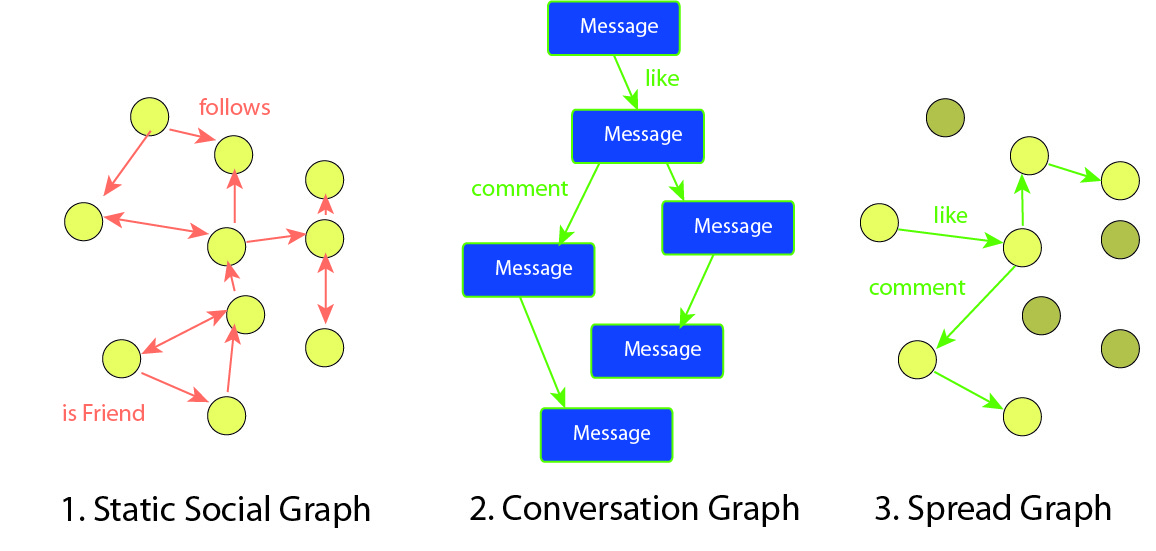
\includegraphics[width=6.2894in,height=3.0004in]{figures/chap3/chapitre3-img9.jpg}
    \caption[3 modèles de réseau]{Les 3 types de graphe classiquement extraits des donn\'ees de r\'eseaux sociaux}
\end{figure}



Dans notre \'etude, le graphe social statique ne pr\'esente pas
particuli\`erement d{\textquoteright}int\'er\^et
puisqu{\textquoteright}il correspond \`a un ensemble de relations peu
affect\'e par les discussions. De plus, nous ne disposons dans le jeu
de donn\'ees Weiboscope que de son \'etat final qui ne t\'emoigne pas
de l{\textquoteright}\'evolution des relations. Nous voulons obtenir
ici les graphes de diffusion sous la forme de conversations
structur\'ees\textbf{~(}graphe directionnelle des \ r\'eponses et
commentaires) de l{\textquoteright}ensemble des messages. Dans un
article paru dans \textit{Nature} \citep{Weng2012}, les chercheurs du
\textit{Centre de Recherche sur les Syst\`emes Complexes} de
l{\textquoteright}Universit\'e d{\textquoteright}Indiana identifient
les caract\'eristiques des m\`emes connaissant le plus de succ\`es (la
plus large diffusion). Un travail de visualisation de m\`emes
identifi\'es par des hashtags sur Twitter leur permet notamment de
mettre \`a jour des motifs particuliers dans la structure des
conversations.



\begin{figure}
    \centering
    \centering
    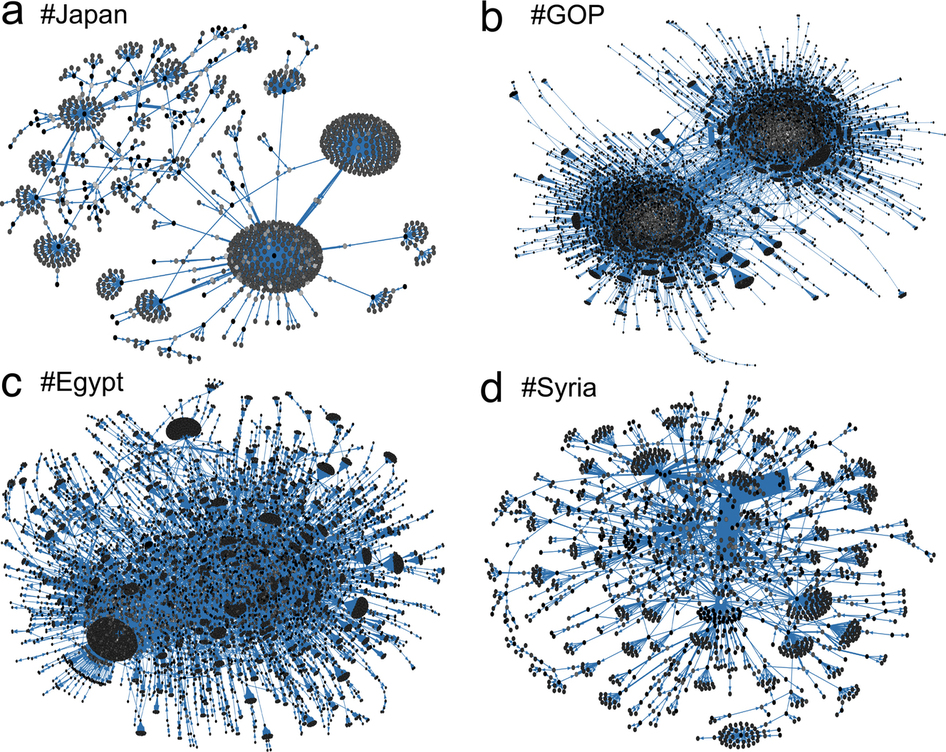
\includegraphics[width=5.5669in,height=4.4224in]{figures/chap3/chapitre3-img10.jpg}

    Nodes represent Twitter users, and directed edges represent retweeted posts that carry the meme. The brightness of a node indicates the activity (number of retweets) of a user, and the weight of an edge reflects the number of retweets between two users. \newline
    (a) The \textit{\#Japan}  meme shows how news about the March 2011 earthquake propagated. \newline
    (b) The \textit{\#GOP} tag stands for the US Republican Party and as many political memes, displays a strong polarization between people with opposing views. \newline
    Memes related to the Arab Spring and in particular the 2011 uprisings in (c) \textit{\#Egypt} and (d) \textit{\#Syria} display characteristic hub users and strong connections, respectively.
    
    \caption{Graphe de diffusion de hashtags sur Twitter d{\textquoteright}apr\`es \citep{Weng2012} }

\end{figure}


Afin de mettre \`a jour le graphe conversationnel entourant les hashtags
s\'electionn\'es sur Sina Weibo, nous avons choisi
d{\textquoteright}extraire la s\'equence d{\textquoteright}interactions
des messages (mentions, retweets) composant chaque m\`eme. Cette
structure de graphe nous permet de repr\'esenter la diffusion de chaque
m\`eme sous forme d{\textquoteright}un graphe contenant un node par
utilisateur et un ensemble de relations correspondant aux \'echanges
visibles dans les textes des messages. Dans un premier temps, le
logiciel \textit{Graphviz }nous a permis d{\textquoteright}obtenir une
repr\'esentation basique du graphe conversationnel afin
d{\textquoteright}avoir un aper\c{c}u sur la nature des conversations
par l{\textquoteright}observation des motifs qui la compose. En effet,
si les deux mesures identifi\'ees \`a l{\textquoteright}\'etape
pr\'ec\'edente (volume de messages et \ volume
d{\textquoteright}\'echanges) nous permettent
d{\textquoteright}effectuer un premier tri parmi les hashtags, cette
premi\`ere visualisation nous permet de consid\'erer la nature des
\'echanges et l{\textquoteright}implication des utilisateurs
d{\textquoteright}apr\`es la structure des motifs conversationnels.
Chaque utilisateur est symbolis\'e par un point et chaque message par
un trait reliant deux utilisateurs. Un motif tr\`es compact refl\`ete
une conversation anim\'ee entre des utilisateurs peu nombreux
\'echangeant beaucoup. A l{\textquoteright}inverse, un motif disparate
refl\`ete des \'echanges plus brefs et morcel\'es.

\begin{figure}
    \centering
    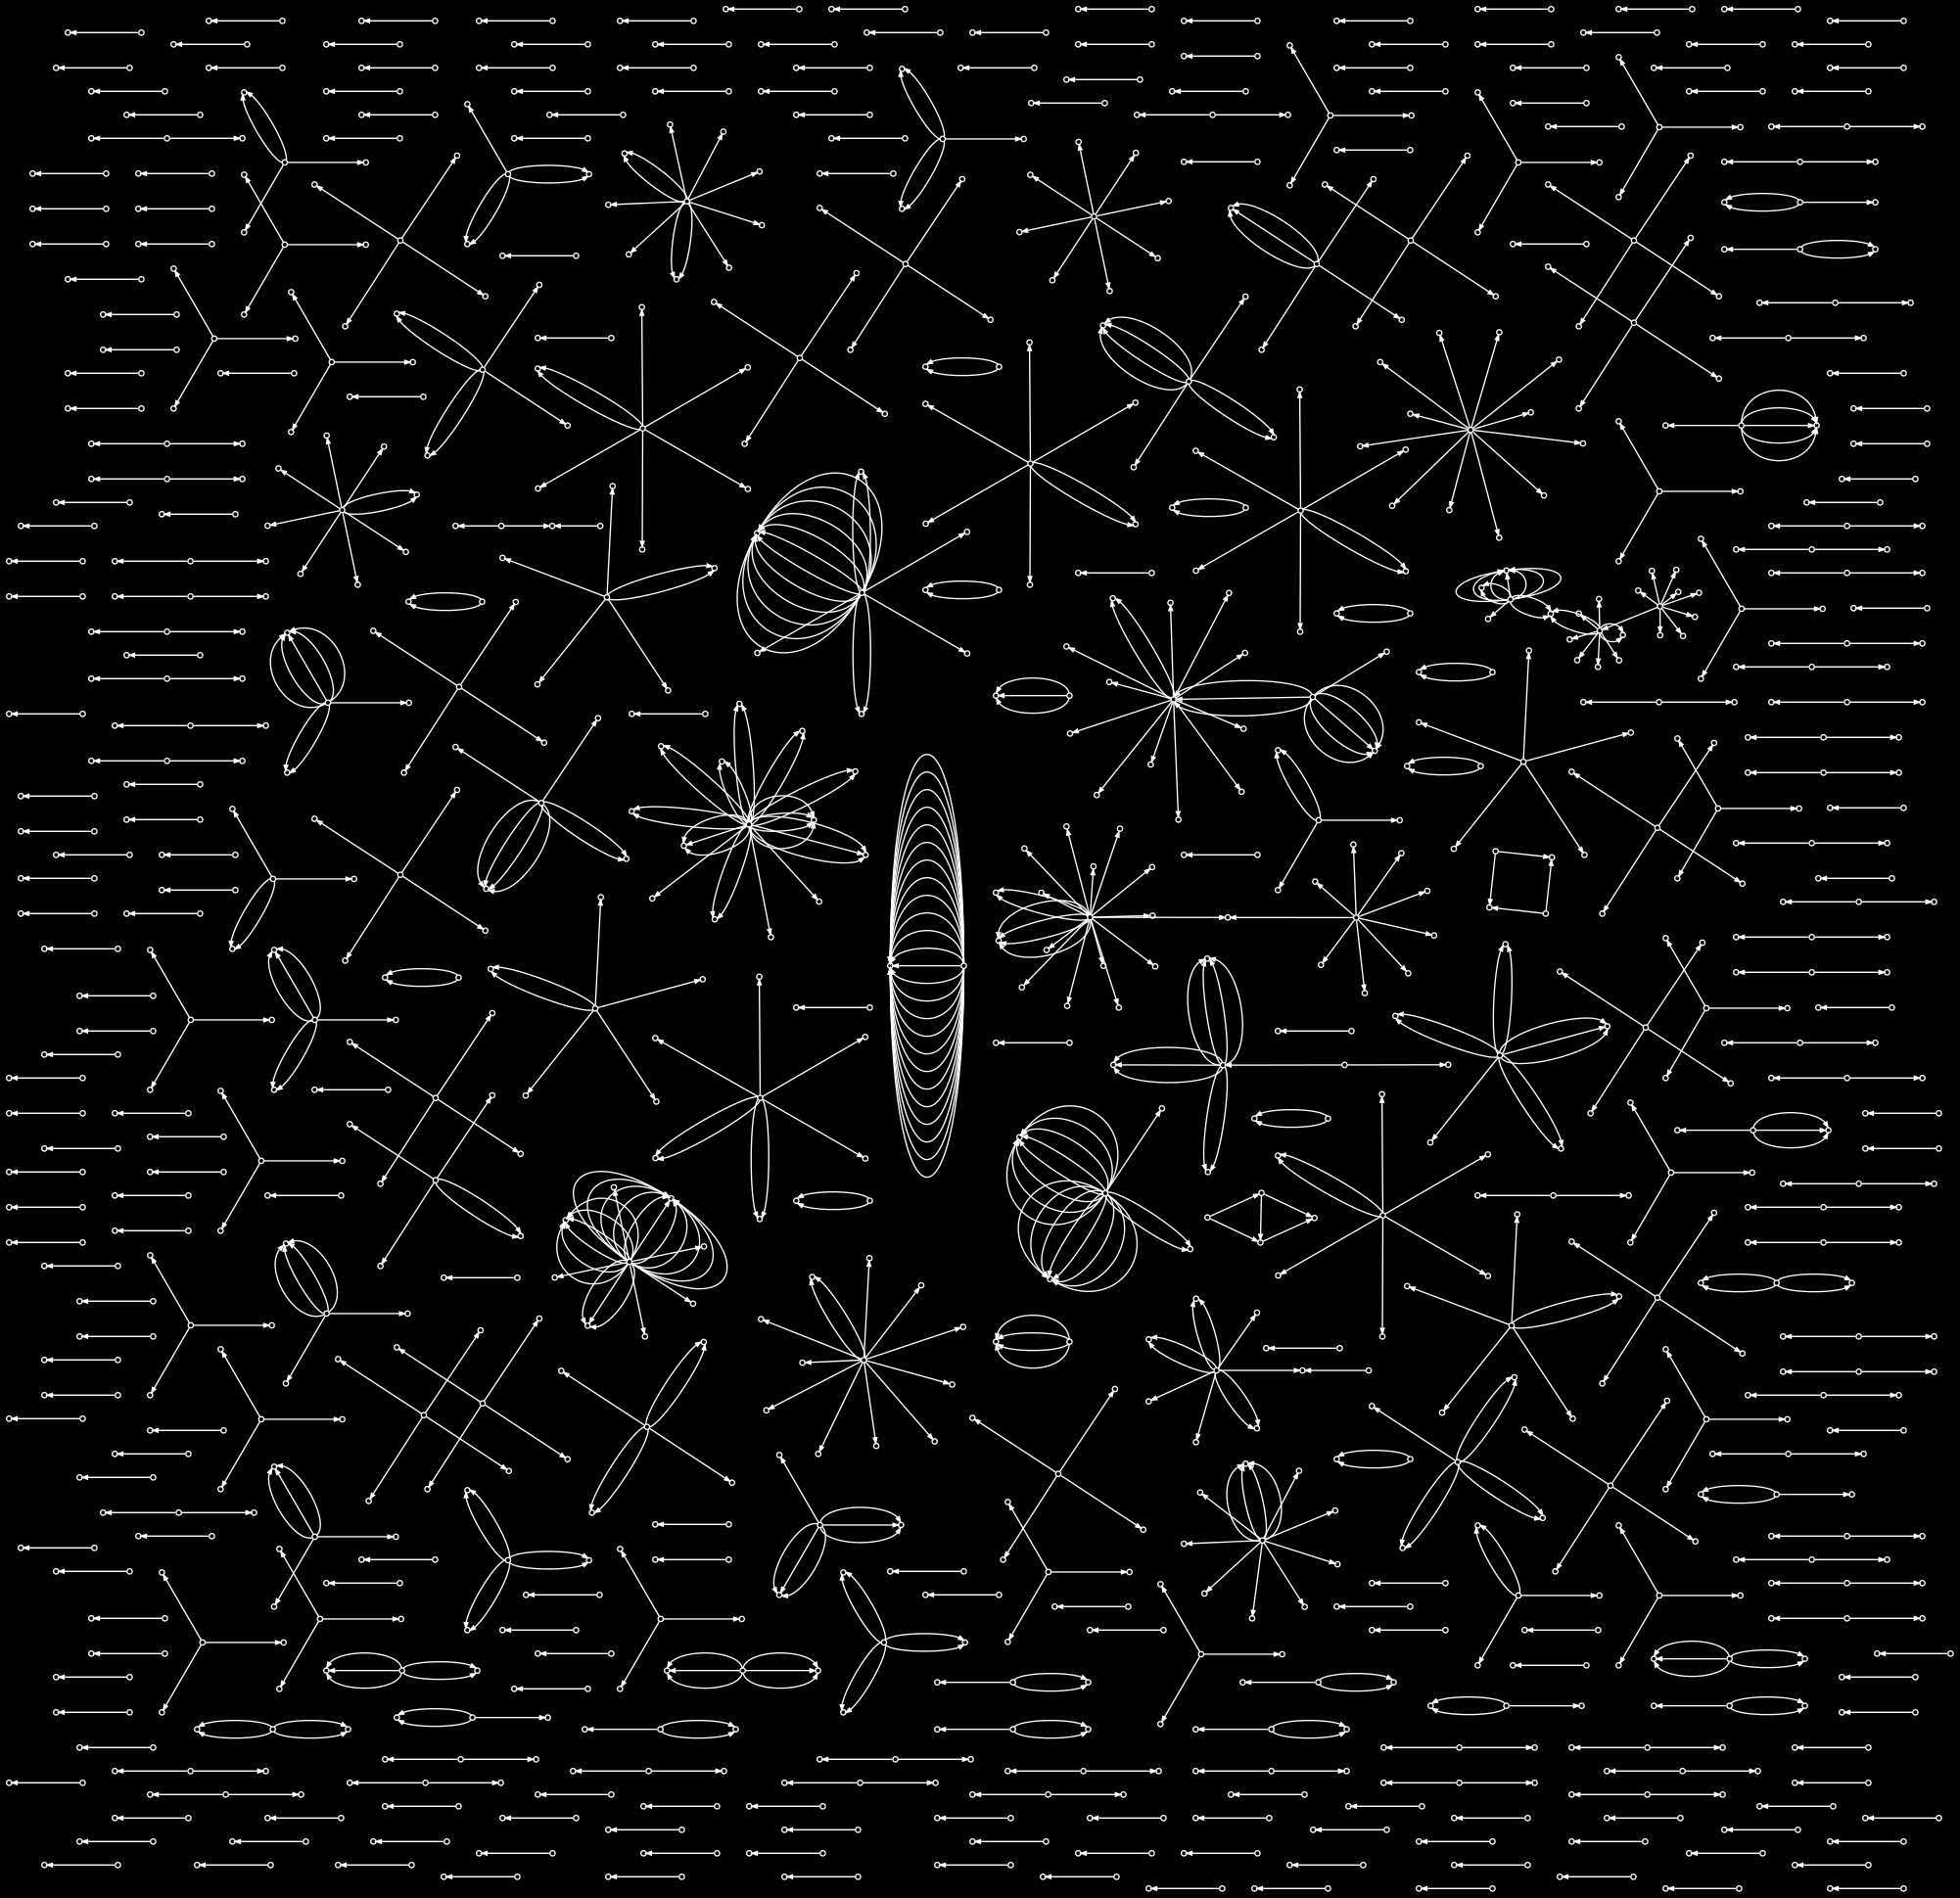
\includegraphics[width=5.5894in,height=5.4224in]{figures/chap3/chapitre3-img11.png}
    \caption[Visualisation simple du hashtag{\textquotedblleft}WeicoPlus{\textquotedblright}] {Fig. Visualisation simple du hashtag{\textquotedblleft}WeicoPlus{\textquotedblright}, un trait repr\'esente un \'echange entre deux utilisateurs}
\end{figure}

\textit{WeicoPlus }est une application mobile permettant
d{\textquoteright}utiliser Sina Weibo. Le hashtag \#WeicoPlus\# est
ajout\'e automatiquement quand les utilisateurs postent des photos
depuis ce service. Ainsi, on remarque que le graphe conversationnel
entourant WeicoPlus se compose essentiellement de messages simples,
mais ne donne pas lieu \`a une conversation structur\'ee - \`a
l{\textquoteright}exception de quelques rapides \'echanges entre un
nombre r\'eduit de personnes.



\begin{figure}
    \centering
    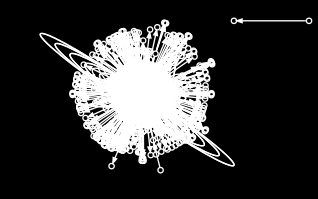
\includegraphics[width=5.0449in,height=3.1559in]{figures/chap3/chapitre3-img12.png}
    \caption[Visualisation simple des conversations autour du hashtag Veuve d{\textquoteright}enfant unique]{Visualisation simple des conversations autour du hashtag Veuve d{\textquoteright}enfant unique}
\end{figure}

A l{\textquoteright}inverse, le hashtag {\textquotedblleft}Veuve
d{\textquoteright}enfant
unique{\textquotedblright}[FF08?]\#[5931?][72EC?][6BCD?][4EB2?]\#[FF09?]cristallise
le d\'ebat en une forme tr\`es dense qui refl\`ete une surench\`ere de
commentaires et d{\textquoteright}actions autour du hashtag, propre
d{\textquoteright}une conversation anim\'ee. 

\subsection[Premiers \'el\'ements d{\textquoteright}analyse: visualisation de m\`emes ]{Premiers \'el\'ements d{\textquoteright}analyse: visualisation de m\`emes }
Les diff\'erents mod\`eles de conversation que nous obtenons dans cette
premi\`ere \'etape se pr\'esentent sous une forme sch\'ematique et peu
d\'etaill\'ee. Afin de comprendre plus en d\'etails les dynamiques
conversationnelles qui les entourent, nous avons choisi de
s\'electionner trois exemples parlants de hashtags dont les graphes
conversationnels pr\'esentent des particularit\'es des mod\`eles de
diffusion dissemblables et organis\'es. Pour chacun
d{\textquoteright}eux, nous allons proc\'eder \`a une analyse plus
d\'etaill\'ee des graphes conversationnels afin de consid\'erer les
diff\'erences entre ces diff\'erents mod\`eles.



\begin{figure}
    \centering
\centering
    \subfloat[Pluie torrentielle \`a Tianjing]{
        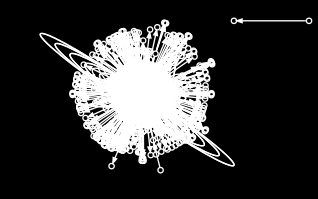
\includegraphics[width=2.3224in,height=1.4449in]{figures/chap3/chapitre3-img13.png}
    }

    \subfloat[Veuve \`a l{\textquoteright}enfant unique]{
        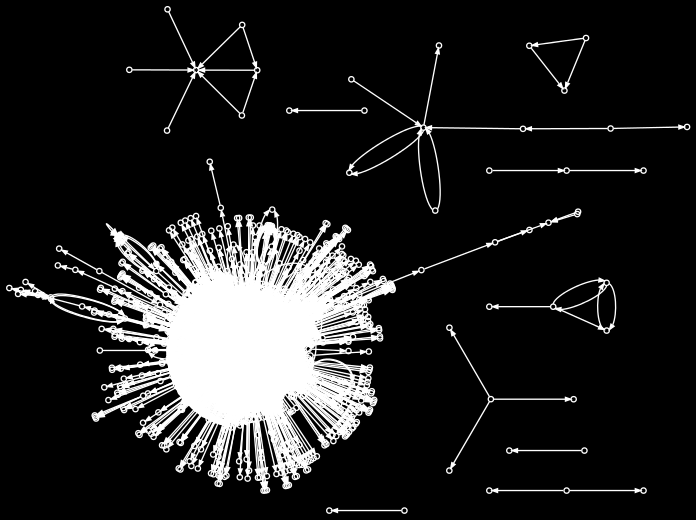
\includegraphics[width=2.3004in,height=1.7224in]{figures/chap3/chapitre3-img14.png}
    }


    \subfloat[Abolition des lois sur la prostitution]{
        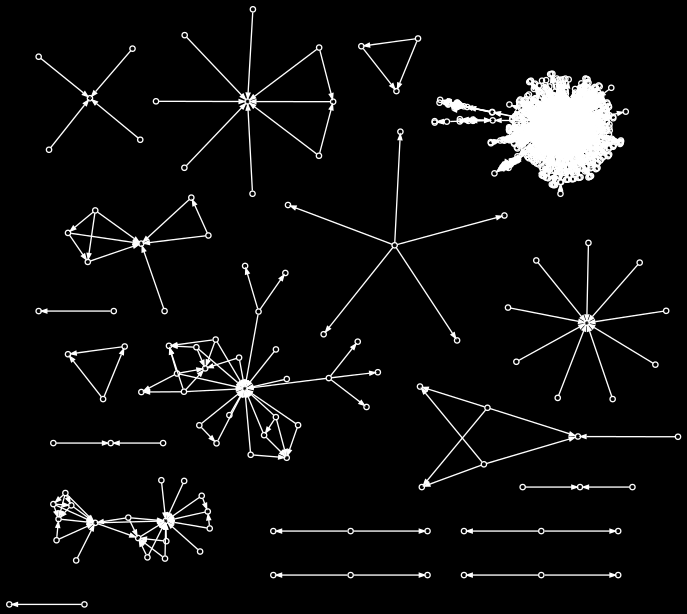
\includegraphics[width=2.1449in,height=1.9224in]{figures/chap3/chapitre3-img15.png}   
    }
  
    \caption{Visualisation des réseaux de conversation}
\end{figure}


Nous voyons que les trois repr\'esentations des graphes ci-dessus
donnent \`a voir des structures plus ou moins morcel\'ees, avec un
ensemble de points et de lignes tr\`es compactes qui repr\'esentent la
majeure partie de la conversation. Afin de visualiser plus
pr\'ecis\'ement les groupes et les dynamiques qui constituent les
discussions autour de chaque hashtag, nous allons utiliser le logiciel
Gephi \citep{Bastian2013} afin d{\textquoteright}examiner de plus pr\`es la
composition de ces graphes. Pour ce faire, Gephi va nous permettre
d{\textquoteright} {\textquotedblleft}\'etaler{\textquotedblright} le
graphe en repositionnant les nodes et en les coloriant pour en
identifier les composantes et les tendances.

Chaque utilisateur est repr\'esent\'e sous la forme d{\textquoteright}un
point. La taille des points correspond \`a l{\textquoteright}importance
de l{\textquoteright}utilisateur dans le r\'eseau tot\ \ al des
\'echanges, caract\'eris\'e par son degr\'e de centralit\'e
interm\'ediaire (\textit{betweenness centrality}), une mesure
topologique correspondant au nombre de plus courts chemins du graphe
passant par cet utilisateur. La couleur est utilis\'ee pour
repr\'esenter la \textit{modularit\'e }du r\'eseau,
c{\textquoteright}est \`a dire le nombre de communaut\'es engag\'ees
dans la conversation d\'efinies comme les cliques
d{\textquoteright}utilisateurs constituant plus de 1\% du r\'eseau
total d{\textquoteright}\'echange \citep{Blondel2008}. La position
des nodes est calcul\'ee gr\^ace \`a l{\textquoteright}algorithme
\textit{Force Atlas 2} \citep{Jacomy2012} utilisant une
mod\'elisation physique o\`u les nodes peu connect\'es entre eux se
repoussent et ceux tr\`es connect\'es s{\textquoteright}attirent.
Ainsi, la proximit\'e de deux nodes sur le graphe t\'emoigne
d{\textquoteright}une proximit\'e lors des conversations,
c{\textquoteright}est \`a dire de l{\textquoteright}existence
d{\textquoteright}un \'echange entre eux (citations, commentaires ou
retweets). Pour davantage de visibilit\'e, certaines conversations
sub-alternes repr\'esentant moins de 1\% du total ont \'et\'e
effac\'ees. Egalement, les nodes poss\'edant un degr\'e inf\'erieur \`a
3 (moins d{\textquoteright}un \'echange avec au moins trois autres
nodes du grahe) ne sont pas repr\'esent\'ees.



\textbf{Exemple 1 : Pluie torrentielle \`a Tianjing}

Le premier m\`eme choisi parle d{\textquoteright}une catastrophe
naturelle, sous la forme d{\textquoteright}une pluie diluvienne qui
s{\textquoteright}est abattue sur la ville de Tianjin durant la nuit du
21 au 22 Juillet 2012. 

\begin{figure}
    \centering
    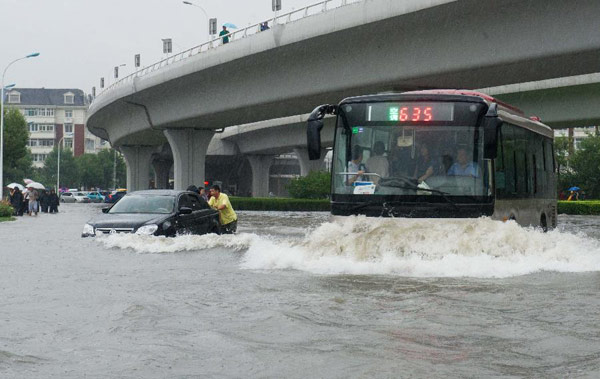
\includegraphics[width=6.0114in,height=3.7894in]{figures/chap3/chapitre3-img16.jpg}
    \caption[Photo de Tianjin durant la pluie torentielle en Juillet 2012]{\textit{Downpour bypasses Beijing, batters neighbor, }in Qinghua News le 2012-07-26 13:29:59, \url{http://news.xinhuanet.com/english/china/2012-07/26/c_131740415.htm} consult\'e le 27 Juin 2014.}
\end{figure}

Ici 4 groupes composent 85\% du graphe, constitu\'es autour de gros
diffuseurs (les nodes les plus gros). Plusieurs groupes semblent
s{\textquoteright}emparer de la conversation mais on voit peu
d{\textquoteright}activit\'e entre les nodes alors que les \'echanges
se d\'eroulent autour de quelques utilisateurs tr\`es centraux. Cela
traduit le fait que peu de personnes ont r\'eellement discut\'e
l{\textquoteright}information et elles se sont simplement content\'es
de la relayer.


\begin{figure}
    \centering
    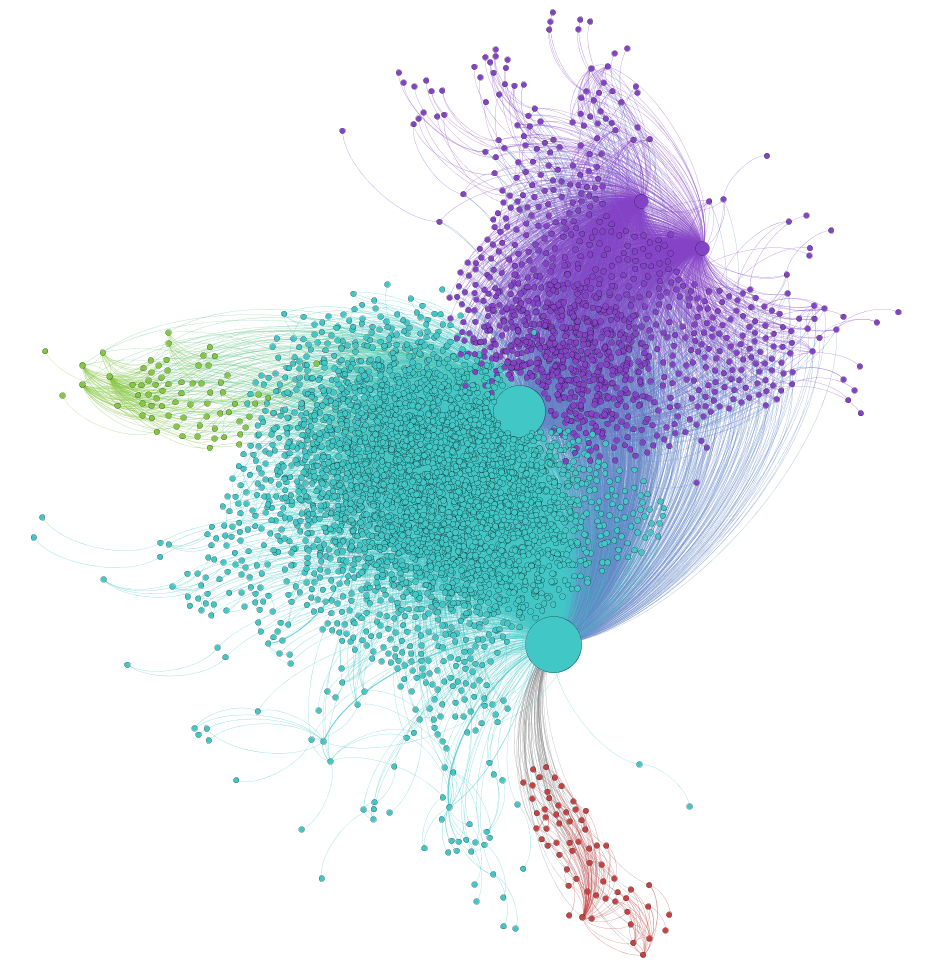
\includegraphics[width=6.0114in,height=6.0114in]{figures/chap3/chapitre3-img17.png}
    \caption{Exemple 1 : Tianjin Baoyu}
\end{figure}

La diffusion d{\textquoteright}un fait divers tr\`es local (il se passe
\`a Tianjing) est entrain\'ee par peu de sources tr\`es importantes
(les quelques nodes de grande taille), vraisemblablement des journaux
et m\'edias locaux qui annoncent la nouvelle (presse, photos-choc
d{\textquoteright}innondations, etc). La conversation est peu active et
tr\`es structur\'ee, nous sommes en pr\'esence d{\textquoteright}un
mod\`ele classique de diffusion de masse.

\textbf{Exemple 2 : Veuve de l{\textquoteright}enfant unique}

Un autre sujet discut\'e par une tr\`es large quantit\'e de personnes
appara\^it sous le terme {\textquotedbl}\textit{shidu
muqin}{\textquotedbl}, forme contract\'ee signifiant
\textit{{\textquotedblleft}m\`ere qui a perdu son enfant
unique{\textquotedblright}
(}[5931?][53BB?][72EC?][751F?][5B50?][5973?][7684?][6BCD?][4EB2?]). Ce
hashtag d\'esigne un ph\'enom\`ene de soci\'et\'e bien connu en Chine
o\`u le deuil de la perte d{\textquoteright}un enfant se double souvent
pour une m\`ere chinoise seule de l{\textquoteright}absence de
ressources pour vivre. En effet, l{\textquoteright}absence de syst\`eme
de retraite fait porter aux enfants la responsabilit\'e de la survie de
la famille. 

Le graphe ici est fait de deux grands groupes composant \`a eux deux
pr\`es de 95\% du graphe total. Les discussions sont tr\`es
polaris\'ees et men\'ees par peu de participants (les nodes les plus
gros sur le graphe). Peu de personnes tr\`es influentes concentrent les
discussions autour d{\textquoteright}eux, accompagn\'es ou suivis
d{\textquoteright}une foule de commentateurs. 

\begin{figure}
    \centering
    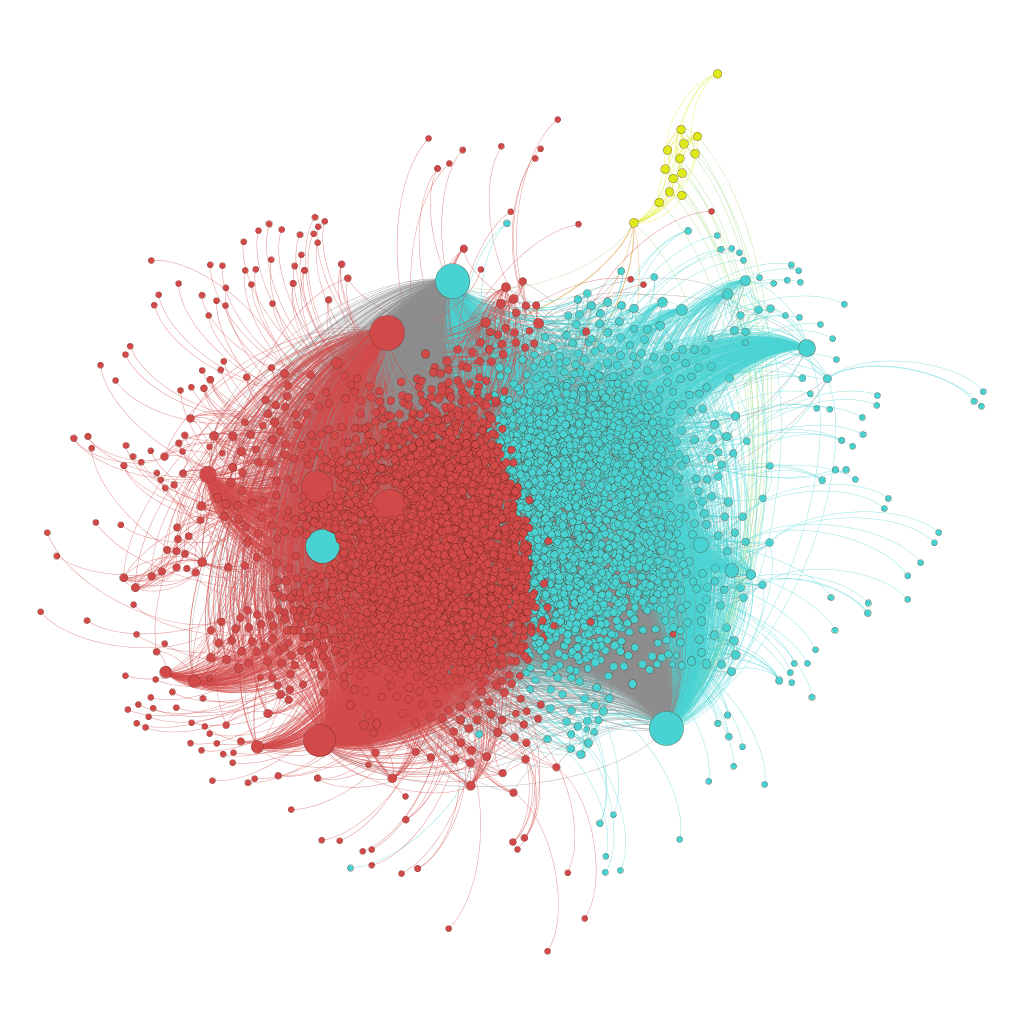
\includegraphics[width=6.0114in,height=6.0114in]{figures/chap3/chapitre3-img18.png}
    \caption{{\textquotedblleft}Shidu Muqin{\textquotedblright}}
\end{figure}


Cet exemple donne \`a voir des groupes bien d\'efinis et tr\`es proches
o\`u plusieurs acteurs majeurs m\`enent la discussion. Les dynamiques
d{\textquoteright}\'echanges autour d{\textquoteright}une question de
soci\'et\'e (la loi de l{\textquoteright}enfant unique en Chine et ses
cons\'equences) s{\textquoteright}articule en groupes distincts sans
pour autant amener \`a des controverses importantes (qui se
traduiraient par des discussions longues et houleuses). Ici, les
leaders d{\textquoteright}opinion font la discussion et la diffusion se
fait au travers d{\textquoteright}eux.

\clearpage
\textbf{Exemple 3 : Abolition des lois sur la prostitution}

Le hashtag \textit{{\textquotedblleft}Abolissons la loi piaowudong
nuzui{\textquotedblright} }est l{\textquoteright}expression
d{\textquoteright}une campagne pour l{\textquoteright}abolition
d{\textquoteright}une l\'egislation scandaleuse sur la prostitution en
Chine. Depuis les ann\'ees 80, la loi chinoise interdit la prostitution
et pr\'evoit la condamnation des deux parties qui
s{\textquoteright}adonnent \`a un \'echange d{\textquoteright}argent.
Baptis\'e \textit{{\textquotedblleft}Piaowudong
nuzui{\textquotedblright}, }cette loi a vu plusieurs cas absurdes
impliquant des viols organis\'es sur mineurs se solder par la
condamnation et l{\textquoteright}emprisonnement des enfants
incrimin\'es. Relay\'es par les journalistes, les scandales \`a
r\'ep\'etition ont \'eclat\'es \`a plusieurs reprises, impliquant
parfois des officiels du Parti souvent blanchis alors que des enfants
\'etaient eux emprisonn\'es. Le graphe des discussions autour de
l{\textquoteright}abolition de cette loi montre que de nombreux groupes
discutent s\'epar\'ement de cette question puisque les premiers 50\% du
graphe sont d\'ej\`a constitu\'es de plus d{\textquoteright}une
quinzaine de clusters. Les groupes sont tr\`es \'eloign\'es entre eux,
n{\textquoteright}entretenant que peu de relations et connaissant une
activit\'e intense.

\begin{figure}
    \centering
    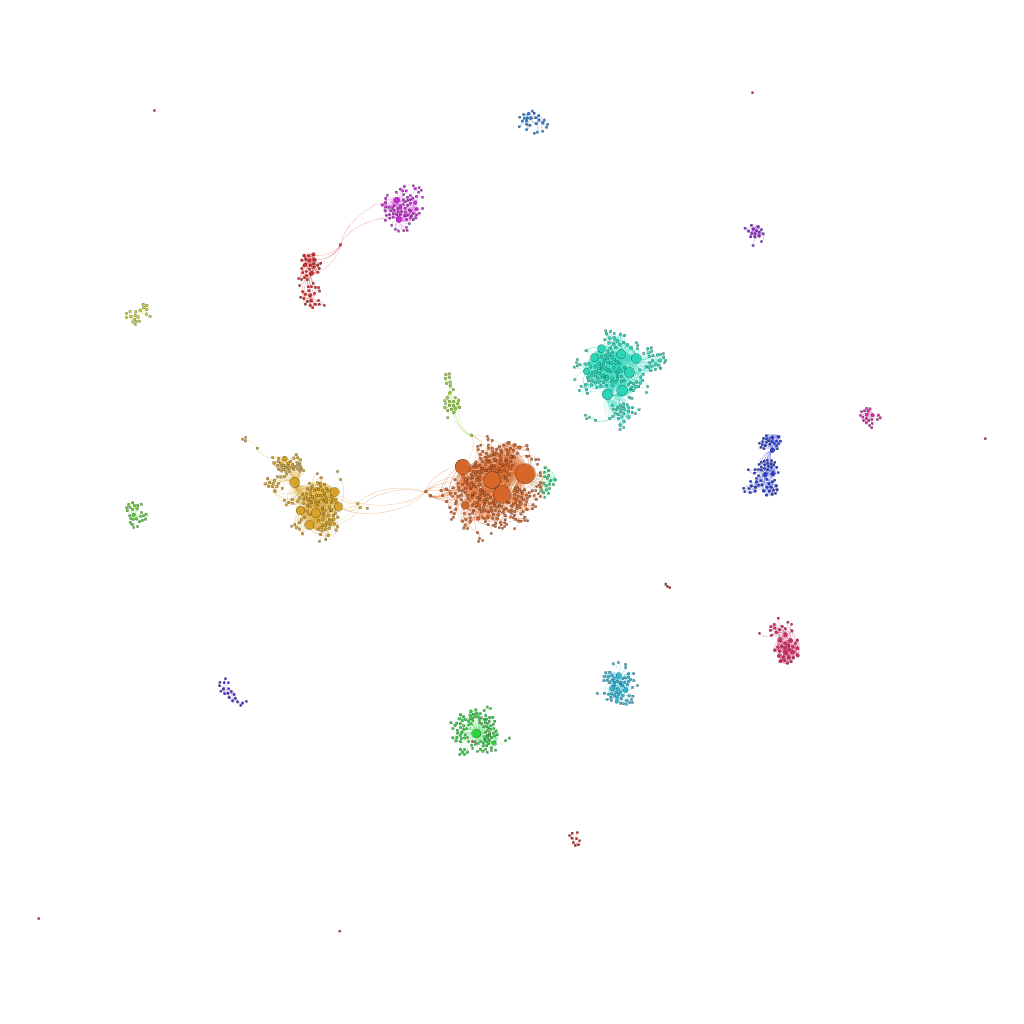
\includegraphics[width=6.0114in,height=6.0114in]{figures/chap3/chapitre3-img19.png}
    \caption{ {\textquotedblleft}Piaowudong nuzui{\textquotedblright}}
\end{figure}

Cet exemple pr\'esente les caract\'eristiques d{\textquoteright}une
conversation tr\`es d\'ecentralis\'ee dans laquelle de nombreux acteurs
diff\'erents prennent part. L{\textquoteright}\'emergence de ce type de
discussion fragment\'ee t\'emoigne d{\textquoteright}un usage
particulier de la discussion sur le r\'eseau social et montre comment
la discussion autour d{\textquoteright}un sujet peut
s{\textquoteright}\'etendre sans afficher de relations directes dans le
m\'edia lui-m\^eme. Ici un agent ext\'erieur (en
l{\textquoteright}occurence un article du journal \textit{Nanfang
Zhoumo }sur le sujet) fait na\^itre la conversation sans pour autant
l{\textquoteright}accaparer et la centraliser. Plus difficilement
d\'etectable et contr\^olable, cette derni\`ere configuration est
typique du m\`eme car elle se d\'eveloppe de fa\c{c}on large et durable
entre des groupes \`a l{\textquoteright}origine peu connect\'es.

Cette premi\`ere visualisation des graphes conversationnels nous permet
d{\textquoteright}explorer quelques types pr\'ecis
d{\textquoteright}\'echanges et d{\textquoteright}en proposer une
premi\`ere lecture. N\'eanmoins, le proc\'ed\'e de visualisation reste
rudimentaire et soul\`eve plusieurs questions que nous nous donnons
pour t\^ache de continuer \`a explorer. Premi\`erement, dans quel
espace a lieu cette repr\'esentation? En \'etalant ainsi ces graphes
conversationnels, quelle action r\'ealisons-nous r\'eellement et quelle
en est la valeur pour l{\textquoteright}analyse? \`A plus forte raison,
quelle est la relation de cette espace du graphe conversationnel avec
les autres formes d{\textquoteright}espace, et plus notamment
l{\textquoteright}espace du r\'eel g\'eographique et
l{\textquoteright}espace de la repr\'esentation par le langage? 

\section{M\'ethodologie de traitement et de visualisation des m\`emes}
L{\textquoteright}\'etude des relations entre ces diff\'erents types
d{\textquoteright}espaces implique donc une m\'ethodologie renouvel\'ee
et le d\'eveloppement d{\textquoteright}outils adapt\'es. Il ne
s{\textquoteright}agit plus simplement d{\textquoteright}\'etudier un
r\'eseau, mais plus pr\'ecis\'ement de s{\textquoteright}interroger sur
les relations entre diff\'erents r\'eseaux, de nature souvent
diff\'erentes. Au-del\`a du r\'eseau multi-calques, nous sommes en
pr\'esence de multiples r\'eseaux poss\'edant des relations communes.

Nous avons donc s\'electionn\'e trois aspects importants des m\`emes que
nous allons tenter de repr\'esenter au mieux afin d{\textquoteright}en
comprendre l{\textquoteright}existence :

\textbf{{}- }\textbf{\textit{langagier }}\textbf{:} le champ
s\'emantique d{\textquoteright}un m\`eme est constitu\'e des mots qui
sont prononc\'es lors de sa diffusion. L{\textquoteright}association de
mots -souvent sous la forme du jeu de mots - est un des propres du
m\`eme et constitue ainsi une part importante de son existence. Ainsi,
le m\`eme produit \`a proprement parler des r\'eseaux de mots en
dessinant des liens entre des signifiants souvent improbables qui en
font souvent le succ\`es \citep{Bauckhage2011}.

\textbf{\textit{{}- conversationnel }}\textit{: }au-del\`a des mots, un
m\`eme se constitue sous la forme d{\textquoteright}un \'echange, une
conversation o\`u les diff\'erents acteurs discutent, commentent et se
saisissent des actions disponibles sur la pateforme web (like,
retweets, etc.) pour converser. Comme nous l{\textquoteright}avons vu
pr\'ec\'edemment, nous pouvons identifier et consid\'erer un graphe
conversationnel cr\'e\'e par le m\`eme en se diffusant.

\textbf{\textit{{}- r\'eel : }}au-del\`a des \'echanges en ligne, ces
discussions poss\`edent une existence physique, premi\`erement sous la
forme de l{\textquoteright}activit\'e \'electrique des machines qui
sont utilis\'ees lors de ce processus. N\'eanmoins, dans
l{\textquoteright}approche d{\textquoteright}une g\'eographie humaine
des \'echanges num\'eriques, nous consid\'ererons ici
l{\textquoteright}existence physique des m\`emes par celle des
utilisateurs - de leurs corps - et non pas des machines.

Afin d{\textquoteright}\'etudier chacun de ces aspects du m\`eme, nous
allons donc proc\'eder \`a la collection et la visualisation de
donn\'ees sur chacun de ces niveaux d{\textquoteright}apr\`es un corpus
de m\`emes s\'electionn\'es.

\subsection[S\'election de m\`emes pour l{\textquoteright}\'etude]{\textmd{\textup{ S\'election de
m\`emes pour l{\textquoteright}\'etude}}}
Choisir un ensemble de m\`emes coh\'erents est une des \'etapes
difficiles de notre recherche. En effet, dans le vaste corpus de
donn\'ees utilis\'ees et plus g\'en\'eralement dans la multitude des
\'echanges quotidiens sur les r\'eseaux sociaux, trouver une prise pour
l{\textquoteright}\'etude n{\textquoteright}est pas une t\^ache
\'evidente. Afin de proc\'eder \`a la s\'election de m\`emes, nous
avons donc choisi d{\textquoteright}utiliser la typologie des
cat\'egories de m\`emes identifi\'ees dans la litt\'erature (voir
partie 2) et d{\textquoteright}en syst\'ematiser
l{\textquoteright}usage sur notre corpus. Ainsi, pour chaque
cat\'egorie, nous avons effectu\'e une recherche m\^elant des sources
parlant des m\`emes et de l{\textquoteright}Internet chinois (journaux,
blogs, encyclop\'edies en ligne, sites ressources), notre propre
exp\'erience du web chinois et notre corpus de donn\'ees disponibles.

Dans un premier temps, nous avons donc identifi\'e pour chaque
cat\'egorie de m\`eme plusieurs \'ev\`enements web de
l{\textquoteright}ann\'ee 2012 sur Sina Weibo comme autant de candidats
pour repr\'esenter l{\textquoteright}ensemble de notre typologie. La
classification de l{\textquoteright}importance des \'ev\`enements web
rev\^et une nature tr\`es diff\'erente selon les diff\'erentes sources.
Une revue de la litt\'erature web sur les
{\textquotedblleft}\'ev\`enements marquant du web social en
2012{\textquotedblright} montre que les contenus \`a caract\`ere
politique et pol\'emique sont consid\'er\'es comme plus importants sur
les sites \`a audience majoritairement occidentale\footnote{ Global
Voices,
\ \ \ \url{http://globalvoicesonline.org/2012/12/07/top-10-chinese-internet-memes-of-2012/,}
consult\'e le 22 Avril 2014 \`a 12:10 ou WSJ
http://blogs.wsj.com/chinarealtime/2012/12/19/the-top-10-chinese-internet-memes-of-2012/,
consult\'e le 22 Avril 2014 \`a 12:10 } alors que les sites plus
sp\'ecialis\'es sur la Chine\footnote{ Danwei
\ \url{http://www.danwei.com/chinas-hottest-styles-of-2012/}
\ consult\'e le 22 Avril 2014 \`a 12:12} prennent davantage en
consid\'eration les ph\'enom\`enes m\'ediatiques commerciaux. Encore
une fois, nous voyons comment les r\'eseaux sociaux chinois sont
repr\'esent\'es comme des ph\'enom\`enes politiques, parfois au
d\'etriment de leur existence comme m\'edia \`a part enti\`ere. Apr\`es
avoir compar\'e ces sources diverses, il nous fallait \^etre s\^ur que
nous disposions d{\textquoteright}une quantit\'e suffisante de
donn\'ees pour traiter le m\`eme choisi. Nous avons donc index\'e les
parties du corpus repr\'esentatives des diff\'erents \'ev\`enements
afin de pouvoir effectuer des \ recherches plein-texte et ainsi
v\'erifier le volume et la qualit\'e des corpus mobilisables pour
chaque m\`eme. Pour ce faire, nous avons mis en place un outil
d{\textquoteright}indexation et de recherche\footnote{ Les technologies
utilis\'ees pour indexer le corpus sont \textit{ElasticSearch }pour le
moteur de recherche et \textit{Kibana} pour le tableau de bord.
\url{http://www.elasticsearch.org} consult\'e le 22 Avril 2014 \`a
12:23} qui nous permet de contr\^oler les diff\'erents param\`etres et
nous assurer de la quantit\'e (taille significative), des dimensions
(dates correctes) et de la qualit\'e du corpus (v\'erification du
contenu d{\textquoteright}un \'echantillon de 100 messages
s\'electionn\'es al\'eatoirement).


\begin{figure}
    \centering
    \includegraphics[width=6.0004in,height=5.078in]{figures/chap3/chapitre3-img20.png}
    \caption[Tableau de bords requêtes par mots-clés] { Ce tableau de bord permet de comparer la qualit\'e de diff\'erentes requ\^etes dans le corpus. Capture d'écran réalisée le 23 Mars 2014 à 16h18}
\end{figure}


Cette \'etape nous a \'egalement permis d{\textquoteright}identifier les
mots-cl\'es les plus appropri\'es pour d\'efinir chaque m\`eme. En
effet, la qualit\'e des archives pour chaque m\`eme d\'epend fortement
de la m\'ethode utilis\'ee pour collecter les donn\'ees. Ici, nous
utilisons la recherche plein texte pour collecter les donn\'ees et nous
devons ainsi nous assurer que notre requ\^ete est bien construite, afin
de minimiser le bruit dans chaque corpus (\'eviter les messages
contenant les m\^eme mots-cl\'es mais sans relations avec le m\`eme). 

Une fois assur\'e qu{\textquoteright}un m\`eme pouvait \^etre
correctement repr\'esent\'e dans un corpus de donn\'ees, nous obtenons
donc une liste r\'eduite de m\`emes \`a \'etudier pour chaque
cat\'egorie.

% \begin{figure}
    \centering
%     \centering
%     \begin{tabular}{c|c|c|c}

%         start & 
%         Name &  
%         type &  
%         keywords \\

%         February 3, 2012 & 
%         Campagne contre les touristes chinois à HK & 
%         Actualité, satire, commentaire social &
%         \zh{蝗蟲天下,蝗虫天下} \\

%         March 21, 2012 &
%         Détournement calligraphie : “Du Fu is very busy" &
%         Absurdiste, humour &
%         \zh{杜甫很忙,李白不服气了} \\

%         April 22, 2012 &
%         Chen Guancheng s'évade et se réfugie à l'ambassade des US &
%         Marketing politique, soutien, pétition &
%         \zh{陈光诚} \\

%         May 30, 2012 & 
%         Rumeur d'un coup d'état des proches de Boxilai (commentaires bloqués) &
%         Marketing politique, soutien, pétition & 
%         \zh{薄熙来,Zhou Yongkang} \\

%         July 13, 2012 &  
%         The Voice : lancement de l'émission TV &
%          Fan clubs, adoration & 
%         \zh{中国好声音, 吴莫愁} \\

%         July 15, 2012 &  
%         Gangnam Style : lancement du clip &  
%         Fan clubs, adoration  &  
%         \zh{鸟叔,江南STYLE} \\

%         August 26, 2012 &
%         Yang Dacai, l'officiel "souriant" et le scandale des montres &   
%         Actualité, satire, commentaire social &  
%         \zh{表叔,表哥,微笑局长,杨达才} \\

%         September 21, 2012 & 
%         Sortie du iPhone5   &
%         Publicité, marketing viral & 
%         \zh{iPhone, 苹果, Apple} \\

%         October 1, 2012 & 
%         Blague : "Yuan Fang, qu'est-ce que tu en penses?"  & 
%         Absurdiste, humour & 
%         \zh{远芳,你怎么看?,我觉得此事有蹊跷,神探狄仁杰} \\

%         October 1, 2012 &
%         Série TV : The Emperor's Harem & 
%         Publicité, marketing viral &
%         \zh{后宫,回家的诱惑,宫 (宫锁心玉)} \\

%         October 11, 2012  &
%         Mo Yan reçoit le Prix Nobel de littérature &
%         Fan clubs, adoration  &
%         \zh{莫言,管谟业,2012诺贝尔文学奖,诺贝尔} \\

%         October 25, 2012 &
%         Ai Weiwei sort son clip "Caonima style"&
%         Actualité, satire, commentaire social &
%         \zh{草泥马style, 艾虎子}\\

%         November 8, 2012 &
%         18ème Congrès du Parti Communiste &
%         Marketing politique, soutien, pétition &
%         \zh{中国共产党第十八次全国代表大会,中共十八大,18大,十八大}\\

%         November 20, 2012 &
%         La sex tape de Lei Zhengfu publiée par un journaliste &
%         Actualité, satire, commentaire social &
%         \zh{雷政富}\\

%         December 3, 2012  &
%         Qiegao : échauffourées autour d'un gâteau du Xinjiang &
%         Actualité, satire, commentaire social &
%         \zh{切糕}\\

%     \end{tabular}
%     \caption[Liste d{\textquoteright}\'ev\`enements web importants pendant l{\textquoteright}ann\'ee 2012] 
% \end{figure}

\subsection{Extraction des graphes et traitement des donn\'ees brutes}
Une fois cette requ\^ete clairement identifi\'ee nous proc\'edons pour
chaque m\`eme \`a l{\textquoteright}extraction d{\textquoteright}un jeu
de donn\'ees contenant l{\textquoteright}ensemble des messages
correspondant \`a la requ\^ete d\'efinie. Ce jeu de donn\'ees est
ensuite compl\'et\'e par l{\textquoteright}ensemble des messages
mentionn\'es mais ne contenant pas le mot cl\'e (commentaires,
r\'eponses, etc.) afin d{\textquoteright}obtenir un ensemble de
messages repr\'esentatifs pour chaque m\`eme.

Nous proc\'edons ensuite au traitement de chaque corpus selon une
s\'erie de proc\'edures d\'efinies comme suit :

\subsubsection{Graphe langagi\`ere (langagier ?)}

Le texte de chaque message est analys\'e de fa\c{c}on \`a ne conserver
que les mots les plus importants. Cela s{\textquoteright}effectue en
cinq \'etapes successives : 

i
\begin{enumerate}
\item La phrase est segment\'ee (analyse de la langue chinoise) pour
obtenir un ensemble de mots du m\`eme.
\item A chacun des mots est associ\'e l{\textquoteright}ensemble des
utilisateurs l{\textquoteright}ayant mentionn\'e.
\item Les mots les plus courants sont enlev\'es afin de r\'eduire le
bruit. La constitution de la liste des mots courants
\textit{(stopwords) }est une \'etape tr\`es importante. La liste que
nous utilisons a \'et\'e cr\'e\'ee \`a partir de diff\'erents corpus
lors d{\textquoteright}exp\'erimentations pr\'ec\'edentes et
augment\'ee de nouveaux mots au fur et \`a mesure.
\item La co-occurence d{\textquoteright}un mot dans une m\^eme phrase
d\'efinit une relation entre ces deux mots.
\item Parmi l{\textquoteright}ensemble de mots-cl\'es ainsi obtenu, nous
conservons les 500 mots les plus utilis\'es (dont les occurences sont
les plus nombreuses) 
\item Nous reconstituons le graphe des relations entre ces 500
mots-cl\'es d{\textquoteright}apr\`es la s\'erie de leur co-occurence :
chaque mot est un node, chaque co-occurence est un edge.
\item L{\textquoteright}ensemble constitue le graphe s\'emantique du
m\`eme, pond\'er\'e mais non dirig\'e.
\end{enumerate}
\textbf{3.4.2.2. Graphe conversationnel}

Pour chaque m\`eme, l{\textquoteright}ensemble des interactions
(mentions, citations et retweets) consituent le graphe conversationnel
o\`u un utilisateur est un node et une interaction est un edge. Le
graphe est dirig\'e car les interactions vont depuis un utilisateur \`a
un autre. 

Une fois l{\textquoteright}ensemble du graphe constitu\'e, nous
d\'eterminons sa modularit\'e et son coefficient moyen de clustering
afin de poss\'eder des informations sur sa structure. Nous calculons
\'egalement la centralit\'e interm\'ediaire (\textit{betweenness
centrality}) pour chaque utilisateur dans l{\textquoteright}ensemble du
graphe. Ensuite, nous identifions les diff\'erentes communaut\'es en
utilisant l{\textquoteright}algorithme dit de Louvain et son
impl\'ementation par Blondel \& al. \citep{Blondel2008}\footnote{
\url{http://perso.crans.org/aynaud/communities/index.html} consult\'e
le 22 Avril 2014 \`a 14:24} qui nous permet d{\textquoteright}attribuer
\`a chaque utilisateur un groupe unique. Enfin, nous r\'eduisons la
taille du graphe final en ne conservant que les utilisateurs ayant
effectu\'e au moins 2 \'echanges - en supprimant les \textit{edges} du
graphe ayant un poids inf\'erieur \`a 2.

Le graphe ainsi constitu\'e correspond aux donn\'ees conversationnelles
du m\`eme.

\subsubsection{Localisation des utilisateurs}

Pour chaque m\`eme, nous souhaitons \'egalement regrouper les
informations de localisation des utilisateurs mentionn\'es ou actifs
dans le m\`eme. Le jeu de donn\'ees \textit{Weiboscope }comprend les
localit\'es mentionn\'ees par les utilisateurs dans leurs profils. Le
nombre de ces localit\'es est restreinte par
l{\textquoteright}interface de Sina Weibo elle-m\^eme \`a :
l{\textquoteright}ensemble des provinces de Chine continentale, Hong
Kong, Macau, Taiwan, {\textquotedblleft}\`a
l{\textquoteright}\'etranger{\textquotedblright} et
{\textquotedblleft}autres{\textquotedblright}. Ainsi, pour chaque
utilisateur nous assignons l{\textquoteright}information g\'eographique
mentionn\'ee par l{\textquoteright}utilisateur dans son profil.

\subsection{Visualisation multi-graphes}
Une fois que l{\textquoteright}ensemble de ces donn\'ees a \'et\'e
extrait et trait\'e, nous pouvons consid\'erer diff\'erents aspects au
sein du m\`eme :

ii
\begin{itemize}
\item Graphe s\'emantique : mots-cl\'es et relations entre les mots
\item Graphe socio-s\'emantique : relations entre les mots et les
utilisateurs
\item Graphe conversationnel : relations et communaut\'es
d{\textquoteright}utilisateurs 
\item Graphe socio-g\'eographique : relations entre les utilisateurs et
les provinces / villes chinoises
\end{itemize}
Nous avons donc plusieurs niveaux de lecture interd\'ependants qui nous
permettent de consid\'erer diff\'erents aspects de chaque m\`eme.
N\'eanmoins, les informations de graphe sont peu claires et
difficilement exploitables sous forme de donn\'ees, \`a
l{\textquoteright}exception d{\textquoteright}une s\'erie de mesures
indicatives sur leurs structures. Afin d{\textquoteright}explorer ces
diff\'erentes relations, il nous faut pouvoir visualiser diff\'erentes
dimensions du m\`eme afin d{\textquoteright}observer les articulations
et ph\'enom\`enes possibles \'emergents de cette lecture. 

Pour r\'ealiser cette cartographie particuli\`ere, il
n{\textquoteright}existe pas d{\textquoteright}outils disponibles
permettant de mettre en relation diff\'erents types de r\'eseaux. Nous
avons donc choisi de d\'evelopper une solution technologique adapt\'ee
\`a nos besoins permettant de consid\'erer sous diff\'erents angles
l{\textquoteright}ensemble de ces graphes et de leurs relations. Les
diff\'erents choix conceptuels et technologiques pr\'esidant au design
de cet outil de visualisation sont d\'etaill\'es ci-apr\`es.

\subsubsection{Choix technologiques}

Les choix technologiques effectu\'es lors de toute cette recherche et
plus particuli\`erement pour cet outil de visualisation ont vocation
\`a faciliter l{\textquoteright}interop\'erabilit\'e et la publication
des r\'esultats (visualisation, code et donn\'ees) en ligne. Egalement,
l{\textquoteright}ensemble de l{\textquoteright}outil de visualisation
se fonde sur HTML5, CSS3 et Javascript qui sont des langages ouverts
issues d{\textquoteright}un travail collectif de
l{\textquoteright}ing\'enierie du Web permettant la r\'eutilisation
partielle ou totale des travaux produits par d{\textquoteright}autres
et contribuant ainsi \`a davantage
d{\textquoteright}interop\'erabilit\'e entre les diff\'erents design
scientifiques de recherche. La mise en forme des donn\'ees utilise la
librairie {\textquotedblleft}Data-Driven Documents{\textquotedblright}
(d3.js)\footnote{ D3js at \url{http://d3js.org/,} consult\'e le 24
Avril 2014 \`a 14:58}, les donn\'ees elles-m\^emes sont stock\'ees en
JSON pour les graphes et GeoJSON pour les donn\'ees cartographiques.

\subsubsection{Espace perceptif, plan projectif et choix
d{\textquoteright}un {\textquotedblleft}layout{\textquotedblright}}

Devant la disparit\'e des donn\'ees en pr\'esence, nous devons donc
construire un espace de repr\'esentation ou plut\^ot une interface de
repr\'esentation propice \`a l{\textquoteright}exploration et la
d\'ecouverte des ph\'enom\`enes dans les relations entre les
diff\'erents graphes. Dans la d\'efinition de cet espace perceptif se
joue la r\'econciliation d{\textquoteright}entit\'es dissemblables (des
utilisateurs, des lieux, des mots, leurs relations mutuelles). La
t\^ache consisterait ainsi \`a r\'econcilier dans le plan de
l{\textquoteright}espace graphique de la visualisation (ici celui de
l{\textquoteright}\'ecran) les diff\'erents espaces o\`u projeter ces
diff\'erents graphes. A l{\textquoteright}image du milieu num\'erique,
l{\textquoteright}existence m\^eme de ce plan r\'econciliant global,
local, r\'eel, symbolique et imaginaire pose question. A la simple
question : {\textquotedblleft}quelle doit \^etre sa
couleur?{\textquotedblright}, une logique commune de lisibilit\'e
r\'epondrait : {\textquotedblleft}blanc ou noir{\textquotedblright},
mais quelle peut en \^etre la justification logique dans
l{\textquoteright}espace de la visualisation? Et que penser du cot\'e
de l{\textquoteright}\'ecran? De quoi est-t-il le bord? D\`es lors que
se pose la question de structurer un espace de perception, nous voil\`a
devant plusieurs difficult\'es formelles majeures.
L{\textquoteright}exigence de rigueur scientifique et surtout
l{\textquoteright}imperm\'eabilit\'e des formats de publications
scientifiques actuelles rajoutent \`a la compexit\'e de cette
entreprise.

Afin de pouvoir consid\'erer les relations entres mots, communaut\'es et
territoires, nous devons dans l{\textquoteright}espace graphique
disponible, il est n\'ecessaire de r\'esoudre plusieurs probl\`emes :

ii
\begin{itemize}
\item Donner \`a voir chaque type d{\textquoteright}entit\'es de
fa\c{c}on reconnaissable (provinces chinoises, communaut\'es, mots)
\item Donner \`a voir les relations entre les diff\'erentes entit\'es
(graphe multiples)
\item Pallier l{\textquoteright}augmentation de la complexit\'e visuelle
et pr\'eserver une lisibilit\'e
\end{itemize}
Nous avons donc choisi de construire un espace sur plusieurs niveaux
hi\'erachis\'es.

\subsubsection{Graphes et interactions}

Le centre de la visualisation est occup\'e par les utilisateurs,
refl\'etant \`a la fois l{\textquoteright}int\'er\^et central de cette
\'etude pour l{\textquoteright}\'etude des processus
d{\textquoteright}individuation et le r\^ole charni\`ere des
utilisateurs dans la structuration des donn\'ees. Plus exactement, nous
avons choisi de regrouper les utilisateurs par communaut\'es afin de
consid\'erer les liens qui les unissaient entre elles et la structure
g\'en\'erale de la discussion plut\^ot que de
s{\textquoteright}int\'eresser aux individus. Les individus sont
symbolis\'es par des points au sein des communaut\'es dont la couleur
indique leur centralit\'e dans le r\'eseau global. 

Notre premi\`ere id\'ee a \'et\'e de repr\'esenter
l{\textquoteright}ensemble des utilisateurs sur une carte pour
comprendre comment s{\textquoteright}agencaient spatialement chacune
des discussions. La premi\`ere \'etape a donc \'et\'e de reconstituer
une carte de la Chine comprenant Taiwan, Hong Kong et Macau. Chacun de
ces territoires poss\`edent une influence m\'ediatique certaine en
Chine et m\'eritent \`a ce titre d{\textquoteright}\^etre
repr\'esent\'e. N\'eanmoins, le statut politique particulier de chacun
de ces territoires nous a oblig\'e \`a reconstituer une carte o\`u ils
figuraient tous. Nous avons choisi d{\textquoteright}aggrandir
l{\textquoteright}\'echelle de Hong Kong et Macau afin
qu{\textquoteright}il soit visible sur la carte. Egalement, nous avons
choisi de ne pas restituer les donn\'ees concernant les utilisateurs
ayant choisi {\textquotedblleft}autres{\textquotedblright} ou
{\textquotedblleft}reste du monde{\textquotedblright} comme leurs lieux
de r\'esidence.

Si la carte se pr\^ete assez bien \`a la visualisation de quantit\'e,
les visualisations de graphe deviennent facilement confuses. Ainsi,
nous avons choisi d{\textquoteright}ajouter une option de visualisation
des provinces sous la forme d{\textquoteright}une liste, au moins toute
aussi parlante. Cela nous permet en plus d{\textquoteright}organiser
cette liste selon diff\'erents crit\`eres afin
d{\textquoteright}\'etudier plusieurs aspects qui peuvent \^etre
int\'eressants.

Le graphe de mots rev\^et ici la forme la plus simple. Les relations
entre les mots sont mat\'erialis\'ees par un graphe utilisant un
algorihme force-based pour disposer les mots entre eux, recr\'eant
ainsi des groupes de mots int\'eressants d{\textquoteright}apr\`es leur
proximit\'e dans les phrases lors des discussions. Un positionnement
des mots selon leur importance (nombre de citations) est \'egalement
disponible \`a loisir.

Afin d{\textquoteright}explorer les diff\'erentes dimensions du graphes,
nous avons \'egalement ajout\'e des interactions qui permettent de
focaliser sur des zones ou des caract\'eristiques pr\'ecises des
graphes. \citep{Bostock2011}

\begin{figure}
    \centering
    \includegraphics[width=6.7213in,height=8.3894in]{figures/chap3/chapitre3-img21.png}
    \caption{Interface d'exploration et de visualisation des données}
\end{figure}
\chapter{R\'esultats et discussions}

Apr\`es avoir d\'efini notre approche m\'ethodologique lors de la phase pr\'ec\'edente, nous allons d\'esormais poursuivre notre \'etude en nous int\'eressant dans le d\'etail \`a chacun des m\`emes choisis. Les choix m\'ethodologiques de cette \'etude cherchent notamment \`a d\'emontrer que les actes de communication ne peuvent simplement se comprendre comme des \'echanges {\textquotedblleft}sociaux{\textquotedblright} mais doivent \^etre appr\'ehend\'es plus largement comme des actes d{\textquoteright}\'enonciation complexes poss\'edant de multiples dimensions s\'emantiques, temporelles, conversationnelles toutes localis\'ees. 

\section{R\'esultats}
Nous allons donc maintenant consid\'erer les diff\'erents aspects de chacun des m\`emes s\'electionn\'es auparavant afin de mieux comprendre comment diff\'erentes lectures peuvent nous informer sur les diff\'erents aspects de chacune de leur diffusion. 

Pour une meilleure commodit\'e de lecture, un nom a \'et\'e attribu\'e \`a chacun des m\`emes \'etudi\'es qui permettra de l{\textquoteright}\'evoquer facilement tout au long du chapitre qui suit. Une pr\'esentation plus d\'etaill\'ee de chaque m\`eme est disponible en annexe de cette th\`ese. 

\begin{table}[t]
  \begin{tabulary}{\textwidth}{c|C}

    \textbf{Nom} &
    \textbf{Description}\\
    \hline \\[-1.5ex]
    \textit{S}\textit{extape}\textit{ } &
    Un scandale d{\textquoteright}adult\`ere concernant un homme politique
    dans la ville de Chongqing dans le centre de la Chine.\\[2ex]

    \textit{The Voice } &
    La premi\`ere saison d{\textquoteright}une \'emission de
    t\'el\'e-crochet musical en Chine.\\[2ex]

    \textit{Qiegao } &
    Un d\'ebat de soci\'et\'e sur la condition du peuple Uyghur suivant un
    fait divers autour d{\textquoteright}une rixe lors
    d{\textquoteright}une vente de g\^ateau.\\[2ex]

    \textit{Dufu} &
    Un m\`eme comique mettant en sc\`ene un po\`ete chinois dans des
    situations burlesques.\\[2ex]

    \textit{Biaoge} &
    Un scandale entourant la collection de montres de marques prestigieuses
    d{\textquoteright}un homme politique de la province du Shaanxi \\[2ex]

    \textit{Moyan} &
    L{\textquoteright}attribution du Prix Nobel de litt\'erature \`a
    l{\textquoteright}\'ecrivain chinois Mo Yan\\[2ex]

    \textit{Yuanfang} &
    La reprise d{\textquoteright}une citation d{\textquoteright}une s\'erie
    t\'el\'evis\'ee sous forme humoristique\\[2ex]

    \textit{Ccp} &
    D\'ebats entourant le 18\`eme Congr\`es du Parti Communiste Chinois\\[2ex]

  \end{tabulary}
  \caption{D\'enomination et description des m\`emes \'etudi\'es}
\end{table}


\subsection[Approches socio{}-s\'emantiques et temporelles de la diffusion]{Approches socio-s\'emantiques et temporelles de la diffusion}

\subsubsection[Structures temporelles]{Structures temporelles}
Dans un premier temps, nous avons choisi de consid\'erer les diff\'erentes structures temporelles des m\`emes. Les figures ci-dessous repr\'esentent chronologiquement le volume de messages \'echang\'es par heure dans chacun des jeux de donn\'ees. La dur\'ee totale des \'echantillons ci-dessous est de 3 semaines. La diminution r\'eguli\`ere de la quantit\'e de messages observ\'es dans les graphes correspond \`a la baisse d{\textquoteright}activit\'e pendant les nuits. 

\begin{figure}[ht]
    \centering
    \subfloat[sextape]{
      \includegraphics[width=6.0087in,height=1.6697in]{figures/chap4/chapitre4-img1.png}
      \label{fig:time-sextape}
    }
    \newline
    \subfloat[dufu]{
      \includegraphics[width=6.0087in,height=1.6697in]{figures/chap4/chapitre4-img2.png}
      \label{fig:time-dufu}
    }
    \newline
    \subfloat[qiegao]{
      \includegraphics[width=6.0087in,height=1.6697in]{figures/chap4/chapitre4-img3.png}
      \label{fig:time-qiegao}
    }
    \newline
    \subfloat[The Voice]{
      \includegraphics[width=6.0087in,height=1.6697in]{figures/chap4/chapitre4-img4.png}
      \label{fig:time-voice}
    }
    \caption{
      Graphe temporel repr\'esentant le volume de messages \'echang\'es sur une dur\'ee de 3 semaines    
    }
\end{figure}
\clearpage

D{\textquoteright}apr\`es ces figures, nous pouvons constater diff\'erentes formes repr\'esentatives : la {\textquotedblleft}breaking news{\textquotedblright} du m\`eme \textit{qiegao} se voit nettement par un d\'epart abrupt de la courbe (Fig. \ref{fig:time-qiegao}) \`a un niveau directement tr\`es \'elev\'e, suivi d{\textquoteright}une retomb\'ee rapide de l{\textquoteright}attention en quelques jours .  

La discussion plus informative autour du proc\`es de l{\textquoteright}homme politique de Chongqing et sa {\textquotedblleft}sextape{\textquotedblright} (Fig. \ref{fig:time-sextape}) croit doucement pour conna\^itre un pic rapide et tr\`es fort de discussion avant de retomber rapidement \'egalement.  

L{\textquoteright}\'emission de t\'el\'evision The Voice est, elle, absolument \'ev\`enementielle et son graphe montre bien le rythme des \'emissions accompagn\'ees de tr\`es peu de discussions entre les \'emissions (Fig. \ref{fig:time-voice}). N\'eanmoins, nous voyons que le volume est nettement plus important avec un pic de plus de 2000 tweets dans une m\^eme heure le soir de la premi\`ere \'emission, d\'epassant tr\`es largement les trois autres m\`emes pr\'esent\'es.  

Le graphe du m\`eme absurdiste {\textquotedblleft}dufu{\textquotedblright} connait une lente mont\'ee d{\textquoteright}attention puis un plateau de plusieurs jours. La blague semble durer et m\^eme conna\^itre un regain d{\textquoteright}int\'er\^et une semaine plus tard et \^etre r\'eguli\`erement mentionn\'e par la suite (Fig. \ref{fig:time-dufu}).  

Proportionnellement, nous constatons que le m\`eme absurdiste est celui qui retient le plus l{\textquoteright}attention, le plus longtemps (Fig. \ref{fig:time-dufu}). A l{\textquoteright}inverse la campagne en ligne de The Voice n{\textquoteright}est qu{\textquoteright}un artefact de l{\textquoteright}\'emission (Fig. \ref{fig:time-voice}) mais draine une audience tr\`es importante pendant un temps restreint. 

\begin{figure}[ht]
    \centering
    
  \includegraphics[width=6.0087in,height=1.6697in]{figures/chap4/chapitre4-img5.png}
  
  \caption{
   Graphe temporel repr\'esentant le volume de messages \'echang\'es  autour du m\`eme \textit{yuanfang} entre le 7 Octobre et le 16 D\'ecembre 2012.
  }
  \label{fig:time-yuanfang}
\end{figure}

La tendance du m\`eme comique \`a durer se v\'erifie \'egalement avec
\textit{yuanfang} (Fig. \ref{fig:time-yuanfang}) qui continue d{\textquoteright}\^etre mentionn\'e
tr\`es r\'eguli\`erement sur une p\'eriode de plusieurs mois (ici du 7
Octobre au 16 D\'ecembre 2012).

A l{\textquoteright}inverse, les informations type {\textquotedblleft}news{\textquotedblright} ont une dur\'ee de vie tr\`es courte, m\^eme lorsqu{\textquoteright}elles sont tr\`es d\'ebattues. Dans le cas de Moyan, on voit un tr\`es fort volume d{\textquoteright}activit\'e (3000 messages par heure au plus haut) mais une disparition quasi-totale des d\'ebats au bout en moins d{\textquoteright}une dizaine de jours (Fig. \ref{fig:time-moyan}).

\begin{figure}
    \centering
    \includegraphics[width=6.0087in,height=1.6697in]{figures/chap4/chapitre4-img6.png}
    \caption{
      Graphe temporel repr\'esentant le volume de messages \'echang\'es autour du m\`eme \textit{moyan} entre le 8 et le 21 Octobre 2012.
    }
    \label{fig:time-moyan}
\end{figure}

\subsubsection[Structures conversationnelles]{Structures conversationnelles}
Les conversations sur Sina Weibo sont faites d{\textquoteright}\'echanges entre les utilisateurs sous la forme de commentaires, de promotion d{\textquoteright}un message ({\textquotedblleft}chuanfa{\textquotedblright} \'equivalent du {\textquotedblleft}retweet{\textquotedblright} de Twitter) ou de r\'eponse au message. Ces diff\'erentes interactions forment dans leur ensemble une large conversation o\`u les utilisateurs interagissent, se parlent, se r\'epondent, discutent en utilisant les diff\'erentes fonctionnalit\'es de la plateforme. En simplifiant ces \'echanges sous la forme de relation dirig\'ee entre deux utilisateurs (\textit{{\textquotedblleft}A interagit avec B{\textquotedblright}}), nous pouvons reconstituer le r\'eseau des interactions que nous visualisons ensuite sous la forme d{\textquoteright}un graphe.  

Dans notre repr\'esentation, chaque utilisateur est un point et chaque interaction correspond \`a un trait. La couleur des points montre l{\textquoteright}appartenance de l{\textquoteright}utilisateur \`a une m\^eme communaut\'e de conversation calcul\'e gr\^ace \`a un algorithme de Louvain \citep{Blondel2008}. La taille des points expriment le nombre total de connexions entrantes et sortantes d{\textquoteright}un utilisateur. La distance entre les groupes d{\textquoteright}utilisateurs est d\'efinie en utilisant l{\textquoteright}algorithme \textit{force} de d3js \citep{Bostock2011} pour calculer leur r\'epulsion : plus les utilisateurs sont proches dans la conversation, plus les points les repr\'esentant sont proches dans le graphe. La forme circulaire du graphe est due aux propri\'et\'es physiques d{\textquoteright}attraction utilis\'ees lors du calcul qui permettent aux diff\'erents nodes du graphe de rester agr\'eger ensemble sans se diss\'eminer. Pour des questions de lisibilit\'e, seuls les 500 utilisateurs les plus actifs ont \'et\'e repr\'esent\'es. Les utilisateurs poss\'edant moins de deux interactions ont \'et\'e supprim\'es pour rendre le graphe lisible. 

\begin{figure}
    \centering
    \subfloat[Sextape]{
      \includegraphics[width=3.0705in,height=2.7913in]{figures/chap4/chapitre4-img7.png}
      \label{fig:users-sextape}
    }
    \subfloat[The Voice]{
      \includegraphics[width=3.0705in,height=2.7913in]{figures/chap4/chapitre4-img8.png}
      \label{fig:users-voice}
    }
    \newline
    \subfloat[Qiegao]{
      \includegraphics[width=3.0705in,height=2.7913in]{figures/chap4/chapitre4-img9.png}
      \label{fig:users-qiegao}
    }
    \subfloat[Dufu]{
      \includegraphics[width=3.0748in,height=2.7913in]{figures/chap4/chapitre4-img10.png}
      \label{fig:users-dufu}
    }
    
  \caption{  
    Graphe conversationnel pour chacun des 4 m\`emes (pour une dur\'ee de 3 semaines)
  }
\end{figure}
\clearpage
Les graphes de conversation permettent d{\textquoteright}identifier des sp\'ecificit\'es et de lire plusieurs indicateurs. Ils rendent notamment bien compte de la taille des conversations, tr\`es variables, ou plut\^ot de la dimension des interactions. On voit que les discussions autour d{\textquoteright}aspects politiques et soci\'etaux connaissent beaucoup plus d{\textquoteright}\'echanges, alors que les deux autres semblent moins importantes. Dans le cas de \textit{The Voice} (Fig. \ref{fig:users-voice}), la conversation est tr\`es structur\'ee autour de peu d{\textquoteright}acteurs qui centralisent les d\'ebats. Le m\`eme absurdiste \textit{dufu} (fig. \ref{fig:users-dufu}) semble \^etre compos\'e d{\textquoteright}utilisateurs tr\`es distants qui ne communiquent entre eux que faiblement ou par petits groupes. La conversation \textit{sextape }autour du fait divers politique se constitue en groupes structur\'es mais plus distants, repouss\'es vers les bords du graphe, montrant l{\textquoteright}existence de nombreux foyers de discussions. A l{\textquoteright}inverse, la discussion de soci\'et\'e \textit{qiegao}\textit{ }autour des peuples du Xinjiang (fig. \ref{fig:users-qiegao}) semble constitu\'e autour d{\textquoteright}un vaste foyer de discussions o\`u viennent s{\textquoteright}agr\'eger de nombreux utilisateurs tr\`es actifs. 

\subsubsection[Structures s\'emantiques]{Structures s\'emantiques}

La dimension lexicale des contenus web pr\'esente une autre approche int\'eressante \`a explorer pour mieux comprendre comment se structure l{\textquoteright}activit\'e lors de la diffusion des m\`emes. La repr\'esentation classique du nuage de mots s{\textquoteright}int\'eresse principalement \`a la quantit\'e de mots en laissant toutefois de cot\'e l{\textquoteright}aspect relationnel de l{\textquoteright}existence des mots qui est pourtant le fondamental de l{\textquoteright}activit\'e symbolique et expressive. Ainsi, nous avons plut\^ot choisi de nous int\'eresser aux r\'eseaux de mots afin de comprendre comment l{\textquoteright}activit\'e en ligne se construit autour de signifi\'es particuliers. 

Les graphes de mots pr\'esent\'es ici sont construits gr\^ace aux co-occurences de mots dans les messages. Si deux mots sont utilis\'es dans un m\^eme message, un \textit{edge} est ajout\'e entre eux, recr\'eant ainsi un graphe pond\'er\'e repr\'esentant une structure s\'emantique relationnelle d{\textquoteright}ensemble entre les mots. La taille des mots repr\'esente le nombre de fois o\`u il sont \'et\'e cit\'es dans l{\textquoteright}ensemble du corpus. Les couleurs d\'efinissent des communaut\'es de mots qui ont \'et\'e calcul\'ees gr\^ace \`a l{\textquoteright}algorithme de Louvain \citep{Blondel2008}. L{\textquoteright}\'epaisseur des traits repr\'esentent l{\textquoteright}intensit\'e des relations (leur nombre de co-occurences dans le corpus). La disposition des mots utilise \'egalement l{\textquoteright}algorithme Force de d3js \citep{Bostock2011} pour calculer la proximit\'e des mots sur la base de l{\textquoteright}intensit\'e de leurs relations. Afin de limiter la taille du graphe, nous avons s\'electionn\'e uniquement les 500 mots les plus utilis\'es.  

Un des biais importants \`a prendre en compte dans la lecture de ces graphes est le fait que les corpus desquels ils sont extraits ont \'et\'e constitu\'es gr\^ace \`a une recherche par mots-cl\'es dans un moteur d{\textquoteright}indexation. Ainsi, les mots les plus pro\'eminents sont ceux qui sont \`a l{\textquoteright}origine de la constitution du corpus. 

\begin{figure}[h!t]
    \centering
    \subfloat[Dufu]{
      \includegraphics[width=3.1661in,height=1.7594in]{figures/chap4/chapitre4-img11.png}
      \label{fig:words-dufu}
    }
    \subfloat[Yuanfang]{
      \includegraphics[width=3.1835in,height=1.7697in]{figures/chap4/chapitre4-img12.png}
      \label{fig:words-yuanfang}
    }
    
  \caption{
    Graphe s\'emantique de co-occurences des mots pour les m\`emes dufu et yuanfang   
  }
\end{figure}

En regardant ces graphes, nous constatons tout d{\textquoteright}abord que les graphe des m\`emes absurdistes (fig. \ref{fig:words-dufu} \& \ref{fig:words-yuanfang})se compose de peu de mots centraux tr\`es fortement connect\'es et entour\'e d{\textquoteright}une myriade de mots de faible densit\'e, correspondant s\^urement aux myriades de d\'eclinaisons qui font le propre de la blague en ligne.  

\begin{figure}[ht]
    \centering
    \subfloat[Sextape]{
      \includegraphics[width=3.1461in,height=1.7504in]{figures/chap4/chapitre4-img13.png}
      \label{fig:words-sextape}
    }
    \subfloat[biaoge]{
      \includegraphics[width=3.2335in,height=1.7961in]{figures/chap4/chapitre4-img14.png}
      \label{fig:words-biaoge}
    }
    
  \caption{
    Graphe s\'emantique de co-occurences des mots pour les m\`emes Sextape et Biaoge
  }
\end{figure}


Les r\'eseaux s\'emantiques de la discussion concernant les faits divers politiques (fig. \ref{fig:words-sextape} \& \ref{fig:words-biaoge}) sont plus structur\'es. Ils sont organis\'es en communaut\'es de mots et de sens plut\^ot bien d\'efinies : une communaut\'e d\'ecrit les d\'etails de l{\textquoteright}affaire (noms de lieux et de personnes, verbes d{\textquoteright}actions), l{\textquoteright}autre se compose d{\textquoteright}adjectifs discutant le caract\`ere houleux de ces histoires, la derni\`ere est faite de mots plus anecdotiques.

\begin{figure}
    \centering
    \subfloat[ccp]{
      \includegraphics[width=3.0843in,height=1.7134in]{figures/chap4/chapitre4-img15.png}
      \label{fig:words-ccp}
    }
    \subfloat[The Voice]{
      \includegraphics[width=3.0752in,height=1.7122in]{figures/chap4/chapitre4-img16.png}
      \label{fig:words-voice}
    }
    
  \caption{
    Graphe s\'emantique de co-occurences des mots pour les m\`emes CCP et The Voice
  }
\end{figure}

 La structure lexicale qui entoure \textit{The Voice }et \textit{CCP }semble tr\`es architectur\'ee, avec des associations plus convenues. Pour \textit{The Voice} (fig. \ref{fig:words-voice}), nous sommes sans surprise en pr\'esence du champ lexical du chant (voix-chant, chant-chanson...) entour\'e par de nombreuses \'emotions et sentiments (arc-en-ciel-amour, trac-courage, etc.). Nous voyons \'egalement que de tr\`es nombreux mots ont \'et\'e propuls\'es sur les bords du graphe car peu reli\'es entre eux ou avec le reste du r\'eseau. Ils sont d{\textquoteright}ailleurs reconnus algorithmiquement comme une seule communaut\'e. Il int\'eressant de constater qu{\textquoteright}on y trouve notamment le vocabulaire propre de l{\textquoteright}\'emission, qui apparemment ne s{\textquoteright}int\`egre pas aux discussions. 

Dans le cas du congr\`es du parti communiste chinois (fig. \ref{fig:words-ccp}), on retrouve \'egalement cette organisation s\'emantique tr\`es hi\'erarchique autour du mot central {\textquotedblleft}parti{\textquotedblright}, avec un ensemble de signifiants issus du programme politique (construction, d\'eveloppement, loi, science, etc.). Un autre \'el\'ement pr\'edominent s{\textquoteright}articule autour du caract\`ere {\textquotedblleft}nouveau{\textquotedblright} (r\'evolution, changement, futur...). Comme dans le cas de \textit{The Voice}, nous sommes en pr\'esence d{\textquoteright}un langage st\'er\'eotyp\'e qui donne lieu \`a un graphe tr\`es structur\'e selon des axes de communication d\'efinis. Proportionnellement, une grande partie des discussions est situ\'e aux fronti\`eres du graphe, tr\`es peu reli\'ee avec le reste de l{\textquoteright}activit\'e.

\begin{figure}
    \centering
    \subfloat[qiegao]{
      \includegraphics[width=2.9248in,height=1.6252in]{figures/chap4/chapitre4-img17.png}
      \label{fig:words-qiegao}
    }
    \subfloat[moyan]{
      \includegraphics[width=2.978in,height=1.6551in]{figures/chap4/chapitre4-img18}.png
      \label{fig:words-moyan} 
    }
    
  \caption{
    Graphe s\'emantique de co-occurences des mots pour les m\`emes Qiegao et Moyan
  }
\end{figure}


\textit{Qiegao} (fig. \ref{fig:words-qiegao}), quant \`a lui, poss\`ede une structure tr\`es centralis\'ee articul\'ee autour d{\textquoteright}un mot-cl\'e pr\'ecis qui relie plusieurs groupes s\'emantiques (communaut\'es de mots par couleurs) autour de lui. On retrouve cette caract\'eristique d{\textquoteright}ensemble dans le graphe de \textit{moyan} (fig. \ref{fig:words-moyan}) m\^eme si la structuration des communaut\'es s\'emantiques est plus accentu\'ee - on peut penser que cela est d\^u aux plus grands volumes de messages \'echang\'es.

\subsection[Structures g\'eographiques et multi{}-graphes]{Structures g\'eographiques et multi-graphes}

Nous avons propos\'e dans cette recherche le terme de milieu num\'erique afin notamment de probl\'ematiser les rapports existants entre les pratiques de la discussion en ligne sur Sina Weibo et l{\textquotesingle}espace de la Chine urbaine moderne. Afin de poursuivre notre interrogation, nous allons d\'esormais observer comment les topologies de diffusion en ligne peuvent se corr\'eler avec la diffusion g\'eographique. La diffusion d{\textquotesingle}un m\`eme suit-elle la hi\'erarchie urbaine classique ou bien la g\'eographie urbaine de l{\textquotesingle}Internet? Existe-t-il des mod\`eles de diffusion selon les types de contenus? Quels sont les \textit{patterns }g\'eographiques d\'ecrits pas la circulation des contenus? 

Pour tenter de r\'epondre \`a ces diff\'erentes questions, nous
disposons de donn\'ees concernant l{\textquoteright}origine des
utilisateurs, d{\textquoteright}apr\`es les provinces dans leur profil
Sina Weibo. En mettant en relations ces informations de profils avec
les diff\'erentes dimensions d\'efinies pr\'ec\'edemment, nous allons
proc\'eder \`a l{\textquoteright}analyse de la diffusion g\'eographique
des m\`emes.

\subsubsection{ Dynamiques des discussions entre provinces}
Nous avons pr\'ec\'edemment extrait pour chaque m\^eme le r\'eseau
conversationnel des interactions entre utilisateurs. En associant
chaque utilisateur \`a sa province d{\textquoteright}origine, \ nous
pouvons reconstituer le r\'eseau des interactions entre provinces. Afin
d{\textquoteright}observer comment les provinces
s{\textquoteright}associent lors de la discussion, nous pr\'esentons le
r\'eseau des interactions sous la forme d{\textquoteright}une graphe
pond\'er\'e et dirig\'e. Un des biais classique de la cartographie des
r\'eseaux sociaux est de reproduire simplement les foyers de
population. Afin de r\'etablir un \'equilibre est de faire appara\^itre
des dynamiques plus particuli\`eres, les r\'esultats ont \'et\'e
pond\'er\'e par le pourcentage de population totale repr\'esent\'ee par
chaque province dans le corpus utilis\'e (Weiboscope). Pour des raisons
de lisibilit\'e, les liens entre les provinces sont dirig\'es non pas
vers la capitale de la province mais vers le \textit{centroid
(barycentre) }de la forme g\'eom\'etrique qui la repr\'esente.
L{\textquoteright}\'epaisseur des traits exprime le volume
d{\textquoteright}\'echanges en pourcentage du total sur la p\'eriode
observ\'ee.

\begin{figure}[H]
    \centering
    \includegraphics[width=4.6606in,height=2.913in]{figures/chap4/chapitre4-img19.png}
    \caption{
      The Voice: Interaction des utilisateurs par province entre le 9 et le 29 Juillet 2012
    }
    \label{fig:geo-voice-t1}
\end{figure}

Dans le cas de \textit{The Voice} (fig. \ref{fig:geo-voice-t1}), nous pouvons voir que
l{\textquoteright}interaction est structur\'e autour
d{\textquoteright}un axe fort entre la province de Zhejiang et P\'ekin.
Cela s{\textquoteright}explique assez simplement par le fait que
l{\textquoteright}\'emission est diffus\'e par Zhejiang T\'el\'evision
dont le compte officiel joue un r\^ole important dans la diffusion et
la promotion de la discussion.

\begin{figure}[H]
    \centering
    \includegraphics[width=4.3858in,height=2.7413in]{figures/chap4/chapitre4-img20.png}    
    \caption{
      The Voice: Interaction des utilisateurs par province entre le 16 et le 17 Juillet 2012
    }
    \label{fig:geo-voice-t2}
\end{figure}

En isolant uniquement le soir de la premi\`ere diffusion (fig. \ref{fig:geo-voice-t2}), on voit que
cette structure s{\textquoteright}accentue encore davantage et que les
interactions se structurent entre le Zhejiang P\'ekin et Shanghai avec
quelques autres axes plus minoritaires.

\begin{figure}[H]
    \centering
    \includegraphics[width=5.7059in,height=3.5661in]{figures/chap4/chapitre4-img21.png}
    \caption{
      Qiegao: Interaction des utilisateurs par province entre le 19 Novembre et le 15 D\'ecembre 2012
    }
    \label{fig:geo-qiegao-t0}
\end{figure}


A l{\textquoteright}inverse, nous voyons que pour \textit{Qiegao} (fig. \ref{fig:geo-qiegao-t0}) les
patterns semblent beaucoup plus diversifi\'es. Guangzhou joue un r\^ole
de diffuseur important et beaucoup d{\textquoteright}informations
converge vers Shanghai et P\'ekin. De nombreuses conversations se
d\'eroulent \'egalement dans l{\textquoteright}ouest de la Chine. En
effet, la discussion concerne ici les peuples Uyghur et on constate que
les habitants du Xinjiang participent davantage \`a la conversation que
dans d{\textquoteright}autres m\`emes. 

\begin{figure}[th]
    \centering
    \subfloat[J1: 3 D\'ecembre 2012]{
      \includegraphics[width=2in,height=1.61in]{figures/chap4/chapitre4-img22.png}
      \label{fig:geo-qiegao-t1}
    }
    \subfloat[J2-3: 4-5 D\'ecembre 2012]{
      \includegraphics[width=2in,height=1.61in]{figures/chap4/chapitre4-img23.png} 
      \label{fig:geo-qiegao-t2}   
    }
    \newline
    \subfloat[J4-6: 6-8 D\'ecembre 2012]{
      \includegraphics[width=2in,height=1.61in]{figures/chap4/chapitre4-img24.png}
      \label{fig:geo-qiegao-t3}
    }
    \subfloat[J7+: 9-16 D\'ecembre 2012]{
      \includegraphics[width=2.8724in,height=1.7961in]{figures/chap4/chapitre4-img25.png}  
      \label{fig:geo-qiegao-t4}
  
    }
    
  \caption{
    Qiegao: Interaction des utilisateurs par province (Jours)
  }
\end{figure}

En consid\'erant l{\textquoteright}\'evolution du m\`eme dans le temps,
nous voyons qu{\textquoteright}il \'emane d{\textquoteright}abord de
Canton (fig. \ref{fig:geo-qiegao-t1}), puis se diffuse \`a P\'ekin et Shanghai (fig. \ref{fig:geo-qiegao-t2}) qui semble jouer un r\^ole d{\textquoteright}amplificateur en le diffusant plus largement (fig. \ref{fig:geo-qiegao-t4}), notamment vers l{\textquoteright}Ouest (fig. \ref{fig:geo-qiegao-t3}). 


\begin{figure}[H]
    \centering
    
    \subfloat[J1: 22 Novembre 2012]{
      \includegraphics[width=1.9587in,height=1.2248in]{figures/chap4/chapitre4-img26.png}
      \label{fig:geo-sextape-t1}
    }
    \subfloat[J2-5: 23-25 Novembre 2012]{
      \includegraphics[width=1.9386in,height=1.2114in]{figures/chap4/chapitre4-img27.png}
      \label{fig:geo-sextape-t2}
    }
    \subfloat[J5+: 26 Nov-15 D\'ec 2012]{
      \includegraphics[width=2.0012in,height=1.2512in]{figures/chap4/chapitre4-img28.png}
      \label{fig:geo-sextape-t3}
    }    
  \caption{
    Sextape: Interaction des utilisateurs par province (Jours)
  }
\end{figure}


\begin{figure}[H]
    \subfloat[J1-3 : 26-28 Aout 2012 ]{
      \includegraphics[width=1.9004in,height=1.1878in]{figures/chap4/chapitre4-img29.png}
      \label{fig:geo-biaoge-t1}
    }
    \subfloat[J4-5 : 29-30 Aout 2012 ]{
      \includegraphics[width=1.9004in,height=1.1878in]{figures/chap4/chapitre4-img30.png} 
      \label{fig:geo-biaoge-t2}
    }
    \subfloat[J5+ : 1-3 Septembre2012]{
      \includegraphics[width=1.9004in,height=1.1878in]{figures/chap4/chapitre4-img31.png} 
      \label{fig:geo-biaoge-t3}
    }
  \caption{
    Biaoge: Interaction des utilisateurs par province
  }
\end{figure}

On retrouve \'egalement ce pattern pour d{\textquoteright}autres faits de soci\'et\'e comme \textit{sextape} ou \textit{biaoge}. Cela illustre bien le r\^ole particulier des m\'edias du sud de la Chine et plus sp\'ecialement celui de Guangzhou (fig. \ref{fig:geo-sextape-t1} \& \ref{fig:geo-biaoge-t1}). Avec une plus grande libert\'e de ton et une plus grande latitude dans leur propos, les m\'edias cantonais sont bien souvent instigateurs d{\textquoteright}affaires importantes alors que les m\'edias p\'ekinois, plus conservateurs joue plut\^ot un r\^ole de diffuseur. 


\begin{figure}[H]
    \subfloat[ Qiegao]{
      \includegraphics[width=1.9016in,height=1.9016in]{figures/chap4/chapitre4-img33.png}
    }
    \subfloat[Sextape]{
      \includegraphics[width=1.9016in,height=1.9016in]{figures/chap4/chapitre4-img34.png}
    }
    \subfloat[Biaoge]{
      \includegraphics[width=1.9016in,height=1.9016in]{figures/chap4/chapitre4-img35.png}
    }
  \caption{
    R\'epartition des utilisateurs par province (en \% du total)
    \label{fig:users-share}
  }
\end{figure}


En observant la r\'epartition des utilisateurs par province pour chacun
de ces trois m\`emes (fig. \ref{fig:users-share}), on remarque que Beijing, Canton, Shanghai ont une
place importante, ainsi que les personnes situ\'ees \`a
l{\textquoteright}\'etranger (Haiwai) et le Zhejiang. N\'eanmoins, le
reste des provinces (repr\'esent\'es ici par
{\textquotedblleft}Others{\textquotedblright} en gris) constitue une
part importante des \'echanges.

% \begin{figure}
%   \includegraphics[width=0.0012in,height=0.0012in]{figures/chap4/chapitre4-img32.png}
% \end{figure}

\begin{figure}[H]
    \centering
    \subfloat[J1: 12 Octobre 2012]{
      \label{fig:geo-moyan-t1}
      \includegraphics[width=1.9004in,height=1.1878in]{figures/chap4/chapitre4-img36.png}
    }
     
    \subfloat[J2: 13 Octobre 2012]{
      \label{fig:geo-moyan-t2}
      \includegraphics[width=1.9004in,height=1.1878in]{figures/chap4/chapitre4-img37.png}
    }

    \subfloat[J3+: 14-21 Octobre 2012]{
      \label{fig:geo-moyan-t3}
      \includegraphics[width=1.9004in,height=1.1878in]{figures/chap4/chapitre4-img38.png}
    }

    \caption{
        Moyan : Interaction des utilisateurs par province   
    }

\end{figure}

Dans le cas de nouvelles plus officielles comme pour \textit{Moyan
}notamment, nous pouvons voir que l{\textquoteright}information
s{\textquoteright}origine g\'en\'eralement de P\'ekin (fig. \ref{fig:geo-moyan-t1}) et se diffuse
vers le sud et le centre (fig. \ref{fig:geo-moyan-t2}). 


\begin{figure}[H]
    \centering
    \includegraphics[width=2.6043in,height=2.6043in]{figures/chap4/chapitre4-img39.png}
  \caption{
    R\'epartition des utilisateurs par province pour Moyan (en \% du total)\\
  }
  \label{fig:geo-moyan-pie}
\end{figure}

La composition des utilisateurs (fig. \ref{fig:geo-moyan-pie}) montre bien que les d\'ebats autour de Moyan sont tr\`es largement domin\'es par P\'ekin avec plus de 50\% de l{\textquoteright}activit\'e impliquant au moins un utilisateur identifi\'e \`a P\'ekin.

Dans le cas des m\`emes absurdistes et comiques, il est int\'eressant de constater qu{\textquoteright}ils ne se construisent pas n\'ecessairement sur les patterns que nous avons pu observer auparavant.

\begin{figure}[H]
    \centering
    \subfloat[dufu]{
      \includegraphics[width=2.9252in,height=1.828in]{figures/chap4/chapitre4-img40.png}
      \label{geo-dufu}
    }
    \subfloat[yuanfang]{ 
      \includegraphics[width=2.9252in,height=1.828in]{figures/chap4/chapitre4-img41.png}
      \label{geo-yuanfang}
    }
    \caption{
        Interaction des utilisateurs par province
    }

\end{figure}


On voit notamment que le m\`eme \textit{dufu } (fig. \ref{geo-dufu}) d\'ebute dans la r\'egion
du Hubei alors que le Liaoning joue un r\^ole cl\'e dans la diffusion de \textit{yuanfang} (fig. \ref{geo-yuanfang}). 

\begin{figure}[H]
    \centering

    \subfloat[(Dufu) J1-2 : 23 au 25 Mars 2012 ]{
      \includegraphics[width=2.9252in,height=1.828in]{figures/chap4/chapitre4-img42.png}
      \label{geo-dufu-t1}
    }
    \subfloat[(Dufu) J3+ : 25 Mars au 15 Avril]{
      \includegraphics[width=2.9713in,height=1.8571in]{figures/chap4/chapitre4-img43.png}
      \label{geo-dufu-t2}
    }
    \newline
    \subfloat[(Yuanfang) 1-2: 15 au 17 Octobre 2012]{
      \includegraphics[width=2.9252in,height=1.828in]{figures/chap4/chapitre4-img44.png}
      \label{geo-yuanfang-t1}
    }
    \subfloat[(Yuanfang) J3+: 18 Oct au 16 D\'ecembre 2012]{
      \includegraphics[width=2.9252in,height=1.828in]{figures/chap4/chapitre4-img45.png}
      \label{geo-yuanfang-t2}
    }
    
    \caption{
        Evolution des interactions des utilisateurs par province pour Dufu et Yuanfang
    }

\end{figure}


En consid\'erant les graphes de temps, on remarque \'egalement que si P\'ekin est bien pr\'esent, les \'echanges des premiers jours se font principalement avec le Hubei (fig. \ref{geo-dufu-t1}) et le Yunnan (fig. \ref{geo-yuanfang-t1}), deux provinces typiquement peu actives. Dans un second temps, l'activité se concentre sur les régions cotières (fig. \ref{geo-yuanfang-t2}).

\begin{figure}[H]
    \centering

    \subfloat[dufu]{
      \includegraphics[width=2.9252in,height=1.828in]{figures/chap4/chapitre4-img46.png}
      \label{geo-same-dufu}
    }
     
    \subfloat[yuanfang]{
      \includegraphics[width=2.9252in,height=1.828in]{figures/chap4/chapitre4-img47.png}
      \label{geo-same-yuanfang}
    }

    \caption{
        Interaction entre utilisateurs de la m\^eme province
    }

\end{figure}

En s{\textquoteright}int\'eressant aux \'echanges qui se d\'eroulent au sein de chaque province (d{\textquoteright}un utilisateur situ\'e dans une province vers un autre utilisateur situ\'e dans la m\^eme province) (fig. \ref{geo-same-yuanfang} \& \ref{geo-same-dufu}),nous constatons que les \'echanges internes sont \'egalement importants au sein des villes principales (Canton, P\'ekin et Shanghai) mais de
nombreuses villes prennent aussi par \`a la discussion (fig. \ref{geo-pie-yuanfang} \& \ref{geo-pie-dufu}). 


\begin{figure}[H]
    \centering

    \subfloat[dufu]{
      \includegraphics[scale=0.5]{figures/chap4/chapitre4-img48.png}
      \label{geo-pie-dufu}
    }
     
    \subfloat[yuanfang]{
      \includegraphics[scale=0.5]{figures/chap4/chapitre4-img49.png}
      \label{geo-pie-yuanfang}
    }

    \caption{
        R\'epartition des utilisateurs par province (en \% du total)
    }

\end{figure}


\subsubsection{Communaut\'es, clusters et groupes de provinces}
Un r\'ecent article du d\'epartement d{\textquoteright}urbanisme de
l{\textquoteright}Universit\'e de Nanjing \citep{Zhen2013} analyse
les relations entre le r\'eseau urbain et le r\'eseau
qu{\textquoteright}il est possible d{\textquoteright}inf\'erer au sein
des relations friends/followers entre les utilisateurs sur Sina Weibo .
Il y est notamment montr\'e que le r\'eseau des relations entre
utilisateurs vient renforcer la hi\'erarchie classique du syst\`eme
urbain en acc\'el\'erant l{\textquoteright}agglom\'eration selon des
mod\`eles spatiaux pr\'e-existants comme celui le pattern des
\textit{{\textquotedblleft}Three majors }\textit{and four
smalls{\textquotedblright} }montrant aussi une diff\'erence tr\`es
marqu\'e entre l{\textquoteright}Ouest et l{\textquoteright}Est.


\begin{figure}[H]
    \centering
    
    \begin{description}
    \item[Three Majors]
      \begin{enumerate}
      \item Pearl River Delta (Guangzhou, Shenzhen)
      \item Beijing-Tianjin-Hebei region (Beijing)
      \item the Yangtze River Delta (Shanghai, Hangzhou, Nanjing)
      \end{enumerate}

    \item[Four Smalls]
      \begin{enumerate}
      \item Chengdu-Chongqing region (Chengdu, Chongqing)
      \item Hercynian region (Fuzhou, Xiamen)
      \item Wuhan (central) region (Wuhan, Changsha)
      \item Northeast China (Shenyang, Harbin, Changchun)
      \end{enumerate}

    \end{description}

   \caption{
      Le mod\`ele urbain chinois du Three majors and four smalls d{\textquoteright}apr\`es \cite{Zhen2013}
    }
\end{figure}


Nous avons donc d\'ecid\'e de comparer ces r\'esultats obtenus depuis le r\'eseau des followers sur Sina Weibo avec les ph\'enom\`enes observ\'es lors de la diffusion de contenus. En effet, si on peut affirmer que le r\'eseau {\textquotedblleft}d{\textquoteright}amis{\textquotedblright} structure les canaux de diffusion de Sina Weibo, ces canaux ne sont pas n\'ecessairement sujets \`a une utilisation fr\'equente et donc \`a l{\textquoteright}actualisation de ces structures. 

Afin d{\textquoteright}observer les patterns form\'es par la diffusion des m\`emes, nous continuons d{\textquoteright}utiliser le r\'eseau des interactions entre provinces des utilisateurs. Afin de d\'etecter les communaut\'es de discussion et identifier les provinces ayant interagit le plus ensemble dans chaque cas, nous soumettons le r\'eseau d{\textquoteright}interactions \`a un algorithme de Louvain \citep{Blondel2008}. Sur les cartes, les couleurs repr\'esentent les diff\'erentes communaut\'es calcul\'ees depuis le r\'eseau d{\textquoteright}interactions. 

\begin{figure}[H]
    \centering

    \subfloat[sextape]{
      \includegraphics[width=3.198in,height=2.0004in]{figures/chap4/chapitre4-img50.png}
      \label{geo-clusters-sextape}
    }
    \subfloat[TheVoice]{
      \includegraphics[width=3.3024in,height=2.063in]{figures/chap4/chapitre4-img51.png}
      \label{geo-clusters-voice}
    } 
    \newline
    \subfloat[Qiegao]{
      \includegraphics[width=3.1878in,height=1.9795in]{figures/chap4/chapitre4-img52.png}
      \label{geo-clusters-qiegao}
    } 
    \subfloat[Dufu]{
      \includegraphics[width=3.5315in,height=2.2087in]{figures/chap4/chapitre4-img53.png}
      \label{geo-clusters-dufu}
    }

    \caption{
        Communaut\'e de provinces dessin\'ees par les \'echanges entre utilisateurs autour de chaque m\`eme 
    }

\end{figure}


\'A la premi\`ere lecture de ces cartes, nous constatons en effet que les provinces de l{\textquoteright}Ouest sont nettement moins engag\'ees que celles de la moiti\'e Est de la Chine. Ce fait refl\`ete que la population des utilisateurs de Weibo est concentr\'ee en majorit\'e dans les grandes villes en d\'eveloppement de la c\^ote et du centre \cite{Fu2013}.  

Le m\`eme absurdiste \textit{dufu} poss\`ede une diffusion plus concentr\'ee (fig. \ref{geo-clusters-dufu}) alors que les discussions politiques semblent regrouper des utilisateurs d{\textquoteright}origines plus diverses (fig. \ref{geo-clusters-sextape} \& \ref{geo-clusters-qiegao}). Nous remarquons \'egalement que Taiwan est absente des discussions plus en lien avec la politique et la soci\'et\'e de Chine continentale, alors qu{\textquoteright}elle est bien pr\'esente dans le cas des m\`emes absurdistes et de l{\textquoteright}\'emission de loisir (fig. \ref{geo-clusters-voice}).  

Devant la diversit\'e de contenus propos\'es par ces cartes, peu de pattern sont d\'ecelables a priori et la circulation des contenus ne semble pas suivre les patterns observ\'es dans les relations friends / followers. 

Ces premi\`eres observations nous montre qu{\textquoteright}il est possible de mieux comprendre les logiques et dynamiques de diffusion des contenus, mais il est n\'eanmoins plus p\'erilleux de consid\'erer les usages du r\'eseau pour en tirer des conclusions sur les dynamiques g\'eographiques d{\textquoteright}ensemble d{\textquoteright}un territoire. De plus, nous ne disposons que de tr\`es peu d{\textquotesingle}aspects {\textquotedbl}g\'eo-localis\'es{\textquotedbl} dans ces donn\'ees (pas de g\'eotag sur chaque message \`a proprement parler) et nous savons que la province d{\textquoteright}origine du profil ne peut \^etre consid\'er\'e comme une source absolument fiable. Les utilisateurs sont en effet libres de la remplir selon leur bon vouloir. De plus, cette information est \'ecrite une fois pour toute et n{\textquoteright}est pas n\'ecessairement mise \`a jour lors des d\'eplacements ou m\^eme d\'em\'enagements des utilisateurs. 

\subsubsection{Dimensions g\'eographiques des graphes socio-s\'emantiques}

Face \`a ces diverses r\'eserves, nous voyons qu{\textquoteright}il est important de recentrer l{\textquoteright}\'etude sur les modes de diffusion et leurs dimensions socio-s\'emantiques. Afin de continuer notre exploration des dynamiques conversationnelles entourant les \'echanges en ligne, nous allons donc nous int\'eresser au croisement de ces diff\'erentes dimensions en consid\'erant les corr\'elations entre les mots, les utilisateurs et les provinces \`a diff\'erents niveaux. 

Tout d{\textquoteright}abord, nous nous proposons d{\textquoteright}observer la distribution des provinces d{\textquoteright}origine des communaut\'es d{\textquoteright}utilisateurs les plus importantes. En s\'electionnant les communaut\'es les plus centrales pour chaque graphe, nous pouvons mieux comprendre comment se r\'epartissent les {\textquotedblleft}influenceurs{\textquotedblright} sur le territoire pour chacun des m\`emes choisis ici.

\begin{figure}[H]
    \centering
    \includegraphics[width=5.9996in,height=2.5004in]{figures/chap4/chapitre4-img54.png}
    \caption{
        Communaut\'e de provinces dessin\'ees par les \'echanges entre utilisateurs autour de Sextape
    }
    \label{fig:sextape-users-pie}
\end{figure}

\begin{figure}[H]
    \centering     
    \includegraphics[width=5.9996in,height=2.5004in]{figures/chap4/chapitre4-img55.png}
    \caption{
        Communaut\'e de provinces dessin\'ees par les \'echanges entre utilisateurs autour de Biaoge
    }
    \label{fig:biaoge-users-pie}
\end{figure}

 

Les communaut\'es form\'ees lors de la discussion autour des m\`emes \`a
teneur plus politique pr\'esentent une grande diversit\'e de
provenances. On voit dans le cas de \textit{biaoge} (fig. \ref{fig:biaoge-users-pie}) et \textit{sextape} (fig. \ref{fig:sextape-users-pie}) que de nombreuses provinces sont repr\'esent\'ees. 


\begin{figure}[H]
    \centering
    \includegraphics[width=5.9996in,height=2.5004in]{figures/chap4/chapitre4-img56.png}
    \caption{
        Communaut\'e de provinces dessin\'ees par les \'echanges entre utilisateurs autour de The Voice
    }
    \label{fig:voice-users-pie}
\end{figure}

 \'A l{\textquoteright}inverse, les communaut\'es d{\textquoteright}utilisateurs les plus impliqu\'ees dans \textit{The Voice } (fig. \ref{fig:voice-users-pie}) ou \textit{Moyan} (fig. \ref{fig:voice-users-pie}) sont pour la plupart localis\'ees \`a Beijing. Par rapport \`a la cartographie pr\'ec\'edente qui montrait les relations fortes avec le Zhejiang pour \textit{The Voice} (fig. \ref{fig:voice-users-pie}), nous voyons ici que la province est tr\`es faiblement repr\'esent\'ee dans les communaut\'es majoritaires. 

\begin{figure}[H]
  \centering
   \includegraphics[width=5.9996in,height=2.5004in]{figures/chap4/chapitre4-img57.png}
    \caption{
        Communaut\'e de provinces dessin\'ees par les \'echanges entre utilisateurs autour de Moyan
    }
    \label{fig:moyan-users-pie}
\end{figure}


Le m\`eme \textit{dufu} (fig. \ref{fig:dufu-users-pie}) montre quant \`a lui un pattern diff\'erent
o\`u les communaut\'es sont plus organis\'ees plus r\'egionalement,
avec moins de diversit\'e d{\textquoteright}origine des utilisateurs
engag\'es dans les discussions.


\begin{figure}
    \centering
    \includegraphics[width=5.9996in,height=2.5004in]{figures/chap4/chapitre4-img58.png}
    \caption{
        Communaut\'e de provinces dessin\'ees par les \'echanges entre utilisateurs autour de Dufu
    }
    \label{fig:dufu-users-pie}
\end{figure}



Une dimension importante du m\`eme absurdiste semble \^etre l{\textquoteright}organisation des conversations en communaut\'es plut\^ot local (utilisateurs de m\^eme province). Une premi\`ere analyse des communaut\'es les plus centrales dans le graphe de \textit{yuanfang} ne nous permet de retrouver ce pattern. Pourtant, en nous int\'eressant aux communaut\'es de seconde et troisi\`eme importance, nous voyons que la plupart se constituent autour de 1 ou 2 provinces seulement.  

Pour continuer notre exploration de l{\textquoteright}existence g\'eographique des relations socio-s\'emantiques dans nos m\`emes, nous allons maintenant nous int\'eresser \`a une seconde dimension qui est celle de la distribution des mots par province. Nous s\'electionnons pour chaque m\`eme les mots les plus centraux du graphe s\'emantique et d\'ecomposons leur usage afin de comprendre la diversit\'e ou l{\textquoteright}unicit\'e de l{\textquoteright}origine des utilisateurs. 

\begin{figure}[H]
    \centering
    \includegraphics[width=6.0087in,height=3.3386in]{figures/chap4/chapitre4-img59.png}
    \caption{
      biaoge : distribution des citations par provinces pour le mot wan signifiant 10000, une quantit\'e ici quantit\'e d{\textquoteright}argent pour une montre.
    }
    \label{fig:biaoge-words-pie-wan}
\end{figure}
 



\begin{figure}[H]
  \centering
  \includegraphics[width=6.0087in,height=3.3386in]{figures/chap4/chapitre4-img60.png}
  \caption{
     biaoge : distribution des citations par provinces pour le mot biao (montre)
  }
  \label{fig:biaoge-words-pie-biao}
\end{figure}


Dans le cas du m\`eme biaoge (fig. \ref{fig:biaoge-words-pie-biao} \& \ref{fig:biaoge-words-pie-biao}), nous voyons que les mots principaux
portent une forte diversit\'e et confirme l{\textquoteright}hypoth\`ese
d{\textquoteright}une diffusion g\'eographique plus large de la
discussion.


\begin{figure}[H]
    \centering

    \subfloat[\textit{zhen}, signifiant {\textquotedblleft}vrai{\textquotedblright}]{
      \includegraphics[scale=0.3]{figures/chap4/chapitre4-img61.png}
    }
    \subfloat[\textit{chang}, signifiant {\textquotedblleft}chanter{\textquotedblright}]{
      \includegraphics[scale=0.3]{figures/chap4/chapitre4-img62.png}
    }
    \newline
    \subfloat[\textit{shengyin}, signifiant "la voix"]{
      \includegraphics[scale=0.5]{figures/chap4/chapitre4-img63.png}
    }
    \caption{
      The Voice : distribution des citations de mots par provinces 
    }
    \label{fig:voice-words-pie}
\end{figure}


\'A l{\textquoteright}inverse, les mots-cl\'es de \textit{The Voice} (fig. \ref{fig:voice-words-pie}) sont
nettement domin\'es par des communaut\'es d{\textquoteright}utilisateurs de P\'ekin ou du Zhejiang qui semblent r\'eellement fixer les termes de la discussion.

\begin{figure}
    \centering
    \subfloat[\textit{zuijin}, signifiant {\textquotedblleft}ces derniers temps{\textquotedblright}]{  
      \includegraphics[scale=0.3]{figures/chap4/chapitre4-img65.png}
    }
    \subfloat[\textit{mang}, signifiant {\textquotedblleft}occupé{\textquotedblright}]{  
      \includegraphics[scale=0.3]{figures/chap4/chapitre4-img66.png}
    }
    \newline
    \subfloat[\textit{dufu}, le nom d'un lettré chinois célèbre]{  
      \includegraphics[scale=0.5]{figures/chap4/chapitre4-img64.png}
    }
    \caption{
      Dufu : distribution des citations de mots par provinces 
    }
    \label{fig:biaoge-words-pie}
\end{figure}

Dans le cas de dufu, les trois mots les plus importants \textit{dufu}, \textit{zuijin} et \textit{mang} qui forment la phrase-m\`eme \textit{dufu est tr\`es occup\'e r\'ecemment }sont tous tr\`es fortement reli\'e \`a la r\'egion de Canton (fig. \ref{fig:biaoge-words-pie}). Cette information, pas forc\'ement pro\'eminente dans les analyses pr\'ec\'edentes, montrent que le d\'eveloppement de ce m\`eme est largement le fait d{\textquoteright}utilisateurs de la r\'egion de Canton. 

% \myTitle{}
% \cite{Guichard2013}

\lettrine{L}{es premiers mots} du premier paragraphe 

Voici un texte avec
\emph{de l'italique},
\textbf{du gras},
\textsc{des petites capitales},
\textsf{des caractères sans empattement},
\texttt{des caractères à chasse fixe},
des mots avec {\small{un corps plus petit}} ou {\large{plus grand}}.

\begin{tabular}{|l|c|r|}
  \hline
  colonne 1 & colonne 2 & colonne 3 \\
  \hline
  1.1 & 1.2 & 1.3 \\
  2.1 & 2.2 & 2.3 \\
  \hline
\end{tabular}


\begin{figure}[h]
   \caption{\label{étiquette} titre}
    \includegraphics[scale=0.5]{images/logoTPT.png}
\end{figure}

\fbox{texte à encadrer}

\selectlanguage{english} % début du passage en typographie anglaise
  Our real "blessings often" appear to us in the shape of pains, losses and disappointments; but let us have patience and we soon shall see them in their proper figures.
\selectlanguage{frenchb} % retour à la typographie française
\end{spacing}
\cleardoublepage


\backmatter
\appendix
\tableofcontents
\addcontentsline{toc}{chapter}{Table des Matières}
\bibliography{refs}
\addcontentsline{toc}{chapter}{Bibliographie}
\listoffigures
\addcontentsline{toc}{chapter}{Liste des Figures}

\part*{Annexes}
% \part{Liste des mèmes}

\end{document}